\documentclass[12pt,a4paper,titlepage]{report}

%%% define a macro \ifpdf para compilacao condicional -- PDF ou
%%% DVI/PS.
%\newif\ifpdf
%  \ifx\pdfoutput\undefined
%  \pdffalse
%\else
%  \pdfoutput=1
%  \pdftrue
%\fi

%%% utilize a acentuacao apropriada para seu sistema: ISO-8859-1 ou UTF-8

%%% caracteres acentuados em ISO-8859-1
%\usepackage[latin1]{inputenc}

%%% caracteres acentuados em UTF-8
\usepackage[utf8]{inputenc}

%%% Suporte para gerar o documento em Portugues e Ingles
\usepackage[english,brazil]{babel}

%%% indenta primeiro paragrafo, estilo brasileiro.
\usepackage{indentfirst}

%%% Enumerações personalizadas
\usepackage{enumerate}

%%% Indice Remissivo
\usepackage{makeidx}

%\ifpdf
%%% somente na versao PDF

%%% Uso de Font Encoding T1 (simulado pelo package AE) -- importante
%%% para a correta hifenizacao de palavras acentudas em Portugues.
%\usepackage{ae}

%%% Para inclusao de graficos
\usepackage[pdftex]{graphicx}

%%% dimensoes do documento
\usepackage[pdftex]{geometry}
%\geometry{a4paper,left=1in,right=1in,top=1cm,bottom=2cm}

%\else
%%% somente na versao DVI/PS

%%% Uso de Font Encoding T1
\usepackage[T1]{fontenc}

%%% Para inclusao de graficos
%\usepackage[dvips]{graphicx}

%%% dimensoes do documento
%\usepackage[dvips]{geometry}
\geometry{a4paper,left=1in,right=1in,top=1in,bottom=1in}

%\fi


%%% pacotes para gerar ambiente de codigo
\usepackage{pacotes/algorithm}
\usepackage{pacotes/algorithmic}

%%% pacote para gerar meus ambientes personalizados
\usepackage{pacotes/ambientes}

%%% pacote para gerar meus comandos personalizados
\usepackage{pacotes/comandos}

%%% pacote para tabelas
\usepackage{tabularx}

%%% pacote para fontes matematicas
\usepackage{txfonts}

%%% pacote para mais tipos de sublinhados
%\RequirePackage[normalem]{ulem}

\title{Apostila de Métodos Numéricos}

\author{Creto A. Vidal\thanks{{http://www.dc.ufc.br}{Departamento de Computação - UFC}}\\
  \texttt{\small {mailto:cvidal@lia.ufc.br}{cvidal@lia.ufc.br}}
}

\date{\today\\
  \small Versão 9.0}

%%% Para a criacao de indice
\makeindex

%%%% preamble ends here
\begin{document}

\maketitle
\thispagestyle{empty}

{%
  \selectlanguage{english}
  \begin{abstract}
    These class notes were organized as a supporting material for the courses of Numerical Methods I and II of Federal University of Cear\' a. They are based on the book, Numerical Methods in C by Shoichiro Nakamura.
  \end{abstract}
}

\begin{abstract}
  Estas notas de aula foram elaboradas para servir de apoio aos cursos de M\' etodos Num\' ericos I e II da Universidade Federal do Cear\' a. Elas s\~ao baseadas no livro, Applied Numerical Mehtods in C by Shoichiro Nakamura.
\end{abstract}

%%% Sumario, lista de figuras e tabelas.
\tableofcontents
%\listoffigures
%\listoftables
%\listalgorithmname

\clearpage

%%% Capitulo 1
\chapter{C\' alculo do Zeros de Fun\c c\~oes N\~ao-Lineares}

%%% Secao 1
\section{Introducao}
%\index{Introdução}%

\begin{itemize}

 \item Raiz de função não linear
 \begin{itemize}
  \item encontrar x tal que $f(x) = 0$.
 \end{itemize}

 \item Exemplos:
 \begin{itemize}
  \item $3x^{4} + 3x^{3} - 16x^{2} + 4x + 1 = 0$.
  \item $tan(x) = tanh(x)$.
 \end{itemize}

\item Motivação para soluções numéricas:
 \begin{itemize}
  \item poucas equações não-lineares apresentam soluções analíticas
 \end{itemize}

\item Métodos numéricos iterativos

\item Todo método tem limitações

\end{itemize}

%%% Secao 2
\section{Metodo da Bissecao}
%\index{Método da Bisseção}%

\begin{itemize}

\item Características do método
 \begin{itemize}
  \item necessita o intervalo que contém a raiz
  \item não necessita continuidade da derivada de $f(x)$
  \item aplica-se a qualquer tipo de equação, inclusive funções não analíticas
  \item baseado no fato de que quando a raiz de $f(x)$ está em [a,c] os sinais nas duas extremidades mudam: $f(a) \times f(c) \leq 0$ (ver figura \ref{fig:bissecao1}).
 \end{itemize}

\begin{figure}[htb]
  %\index{figura da bisseção}%
  \setlength{\abovecaptionskip}{20pt}
  %%% o valor default de \abovecaptionskip definido para a classe
  %%% article e de 10pt.
  \centering
  %%% VIDE ABAIXO COMENTARIO SOBRE USO DE DIRETORIOS NO PATHNAME
  %%% DOS ARQUIVOS INCLUIDOS.
  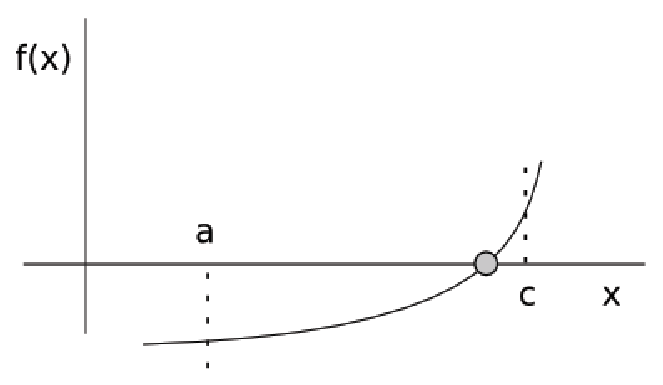
\includegraphics[scale=0.5]{capitulos/capitulo1/figuras/bissecao1.eps}
  \caption{Função $f(x)$ com isolamento [a,c].}
  \label{fig:bissecao1}
\end{figure}

\end{itemize}

\begin{algorithm}{htbp}

  \caption{Método da Bisseção}

  \begin{algorithmic}
    \STATE \textbf{Inicialização:} $i=0$, $a_{0}=a$, $c_{0}=c$

    \STATE \textbf{Iteração i:}

    \begin{enumerate}
     \item tamanho do intervalo, $\displaystyle s_{i} = c_{i}-a_{i} = \frac{s_{0}}{2}^{(i)}$
     \item Se $ \displaystyle \frac{s_{i}}{2} \leq \textit{\textbf{tol}} $

      $ \displaystyle \textit{x}_{i} = \frac{(a_{i} + c_{i})}{2} $

      $ \displaystyle \textit{err}_{i} = \frac{s_{i}}{2} = {\frac{s_{0}}{2}}^{(i+1)} $

      sai

      Se $ \displaystyle \frac{s_{i}}{2} > \textit{\textbf{tol}} $, vá para 3.

      \item Calcule

      $ \displaystyle b_{i} = \frac{(a_{i} + c_{i})}{2} $

      $ f(a_{i}) \ast f(b_{i}) $

      $ f(b_{i}) \ast f(c_{i}) $

      \item Se $ f(a_{i}) \ast f(b_{i}) \leq 0 $, (raiz em [$a_{i}$, $b_{i}$])

      faça $i = i + 1$, $c_{i} = b_{i-1}$, vá para 1.

      Se $ f(b_{i}) \ast f(c_{i}) \leq 0 $, (raiz em [$b_{i}$, $c_{i}$]),

      faça $i = i + 1$, $a_{i} = b_{i-1}$, vá para 1.

    \end{enumerate}

  \end{algorithmic}

\end{algorithm}

\begin{displaymath}
 \frac{c_{0} - a_{0}}{2^{n+1}} \leq \textit{\textbf{tol}}
\end{displaymath}
\begin{displaymath}
 \Rightarrow \frac{c_{0} - a_{0}}{\textit{\textbf{tol}}} \leq 2^{(n+1)}
\end{displaymath}
\begin{displaymath}
 \Rightarrow n + 1 \geq \log_{2}\left( \frac{c_{0}-a_{0}}{\textit{\textbf{tol}}} \right)
 = \frac{ \ln \left( \frac{c_{0}-a_{0}}{\textit{\textbf{tol}}} \right) }{\ln(2)}
\end{displaymath}
\begin{displaymath}
 \Rightarrow n \geq \ln\left( \frac{c_{0}-a_{0}}{ln(2)} - 1 \right)
\end{displaymath}

\textbf{Observações:}

\begin{itemize}
\item após \textbf{n} iterações o tamanho do intervalo é $\displaystyle \frac{(c-a)_{0}}{2^{n}}$

\item o erro máximo na n-ésima iteração é
$\displaystyle \textbf{err}_{n} = \frac{s_{n}}{2} = \frac{s_{0}}{2^{(n+1)}}$

\item Se \textit{\textbf{tol}} é dada, o número de iterações necessárias é dado por
\begin{displaymath}
\displaystyle \frac{c_{0}-a_{0}}{2^{(n+1)}} < \textit{\textbf{tol}}
\end{displaymath}
ou
\begin{displaymath}
n \geq \frac{\ln\left( \frac{c_{0}-a_{0}}{\textit{\textbf{tol}}} \right)}{\ln(2)-1}
\end{displaymath}
\end{itemize}

\begin{example}

\begin{itemize}
\item $ c_{0} - a_{0} = 1$ e $\textit{\textbf{tol}} = 0.0001 $

\item $ n \geq \frac{\ln\left(\frac{1}{0.0001} \right)}{\ln(2)} - 1 = 13.28 - 1 = 12.28 $

\item $n = 13$ ( $14^{a}$ iteração )

\end{itemize}

\end{example}

\begin{example}
 A raiz de $ f(x) = e^{x} - x = 0 $
está no intervalo [0,2]. Encontre uma aproximação da raiz dentro de uma tolerância de 0.01 pelo método da bisseção.

\textbf{Solução:}

\begin{enumerate}
 \item Solução exata: $ e^{x} - 2 = 0 \Rightarrow e^{x} = 2 \Rightarrow x = \ln 2 = 0.6931 $
 \item Solução pelo método da bisseção (ver tabela \ref{tab:bissecao})

\begin{table}[htp]
\footnotesize
	\centering
		
		\begin{tabular}{|c|c|c|c|c|c|c|c|}
		\hline		
		\textbf{Iteração} & \textbf{a} & \textbf{b} & \textbf{c} & \textbf{f(a)} & \textbf{f(b)} & \textbf{f(c)} & \textbf{Erro máximo}\\
		\hline \hline 
		0 & 0 & 1 & 2 & -1 & 0.7182 & 5.3890 & 1\\
		\hline 
		1 & 0 & 0.5 & 1 & -1 & -0.3512 & 0.7182 & 0.5\\
		\hline 
		2 & 0.5 & 0.75 & 1 & -0.3512 & 0.1170 & 0.7182 & 0.25\\
		\hline 
		3 & 0.5 & 0.625 & 0.75 & -0.3512 & -0.1317 & 0.1170 & 0.125\\
		\hline 
		4 & 0.625 & 0.6875 & 0.75 & -0.1317 & -0.0112 & 0.1170 & 0.0625\\
		\hline 
		5 & 0.6875 & 0.7187 & 0.75 & -0.0112 & 0.0518 & 0.1170 & 0.03125\\
		\hline  
		6 & 0.6875 & 0.7031 & 0.7187 & -0.0112 & 0.0200 & 0.0518 & 0.015625\\
		\hline 
		7 & 0.6875 & 0.6953 & 0.7031 & -0.0112 & 0.0043 & 0.0200 & 0.0078125\\
		\hline
		\end{tabular}
	%\caption{Iterações do método da bisseção}
	\caption[Exemplo de iterações do método da bisseção]{A oitava aproximação da raiz é $x = 0.6953$ o máximo erro possível é $0.0078 < 0.01$.}
	\label{tab:bissecao}
\end{table}

\end{enumerate}

\end{example}

\textbf{Notas:}

\begin{enumerate}
 \item O critério $f(a) \ast f(b) \leq 0$ é satisfeito sempre que o número de raízes no intervalo for ímpar. Assim o método encontra uma das raízes (ver figura \ref{fig:bissecao2}).

\begin{figure}[htb]
  %\index{figura da bisseção}%
  \setlength{\abovecaptionskip}{20pt}
  %%% o valor default de \abovecaptionskip definido para a classe
  %%% article e de 10pt.
  \centering
  %%% VIDE ABAIXO COMENTARIO SOBRE USO DE DIRETORIOS NO PATHNAME
  %%% DOS ARQUIVOS INCLUIDOS.
  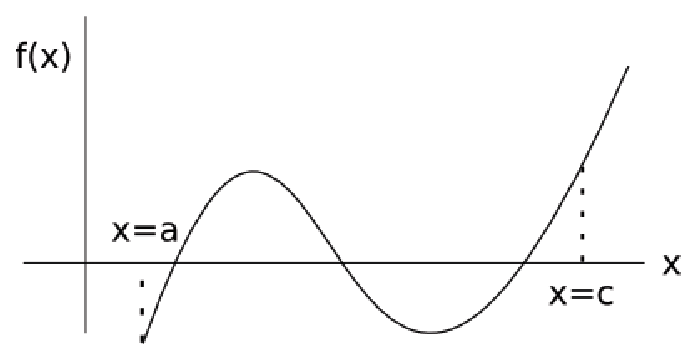
\includegraphics[scale=0.8]{capitulos/capitulo1/figuras/bissecao2.eps}
  \caption{Função $f(x)$ com número de raízes ímpar.}
  \label{fig:bissecao2}
\end{figure}

\item O método da bisseção não pode encontrar um par de raízes duplas porque a função tangencia o eixo x (ver figura \ref{fig:bissecao3}).

\begin{figure}[htb]
  %\index{figura da bisseção}%
  \setlength{\abovecaptionskip}{20pt}
  %%% o valor default de \abovecaptionskip definido para a classe
  %%% article e de 10pt.
  \centering
  %%% VIDE ABAIXO COMENTARIO SOBRE USO DE DIRETORIOS NO PATHNAME
  %%% DOS ARQUIVOS INCLUIDOS.
  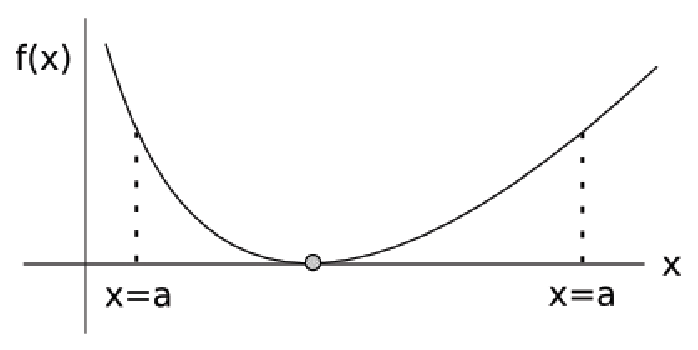
\includegraphics[scale=0.8]{capitulos/capitulo1/figuras/bissecao3.eps}
  \caption{Função $f(x)$ com um par de raízes duplas.}
  \label{fig:bissecao3}
\end{figure}

\item O método pode confundir um ponto de singularidade com uma raiz. Para evitar que isso aconteça, verifique se $|f(c) - f(a)| = 0 $ a medida que o processo avança (ver figura \ref{fig:bissecao4}).

\begin{figure}[htb]
  %\index{figura da bisseção}%
  \setlength{\abovecaptionskip}{20pt}
  %%% o valor default de \abovecaptionskip definido para a classe
  %%% article e de 10pt.
  \centering
  %%% VIDE ABAIXO COMENTARIO SOBRE USO DE DIRETORIOS NO PATHNAME
  %%% DOS ARQUIVOS INCLUIDOS.
  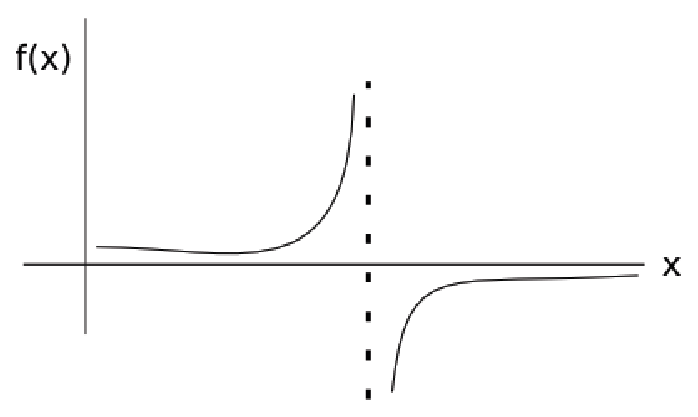
\includegraphics[scale=0.8]{capitulos/capitulo1/figuras/bissecao4.eps}
  \caption{Função $f(x)$ onde pode haver confusão entre ponto de singularidade com uma raiz.}
  \label{fig:bissecao4}
\end{figure}

\item Quando não se tem informação prévia sobre valores aproximados das raízes, uma maneira fácil de encontrar intervalos contendo raízes é imprimir uma tabela da função para valores de x igualmente espaçados ou plotar a função utilizando computação gráfica.

\end{enumerate}

\textbf{Nota falada do professor:}

\begin{itemize}
 \item Antes de iniciar o método deve-se identificar por tabela ou gráfico os intervalos que contêm raízes.

 \item O método encontra a raiz de uma função se a raiz existir no intervalo dado.

 \item O método encontra a raiz de uma função mesmo quando a função não é analítica.

 \item O método não distingue entre uma raiz e um ponto de singularidade.
\end{itemize}

%%% Secao 3
\section{Métodos da Posição Falsa e da Posição Falsa Modificado}
%\index{Métodos da Posição Falsa e da Posição Falsa Modificado}

\subsection{Método da Posição Falsa}

\begin{enumerate}
 \item Esse método difere do método da bisseção apenas na forma como o ponto \underline{b} é calculado.

\begin{figure}[htb]
  %\index{figura da posição falsa}%
  \setlength{\abovecaptionskip}{20pt}
  %%% o valor default de \abovecaptionskip definido para a classe
  %%% article e de 10pt.
  \centering
  %%% VIDE ABAIXO COMENTARIO SOBRE USO DE DIRETORIOS NO PATHNAME
  %%% DOS ARQUIVOS INCLUIDOS.
  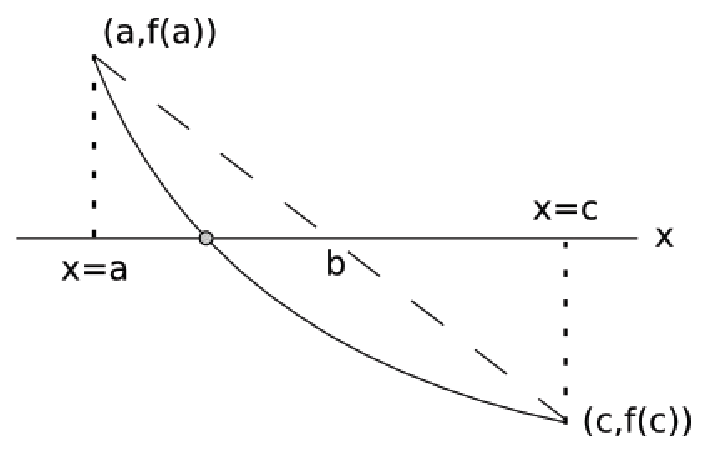
\includegraphics[scale=0.8]{capitulos/capitulo1/figuras/posicaofalsa1.eps}
  \caption{Método da Posição Falsa}
  \label{fig:posicaofalsa1}
\end{figure}

\begin{equation}
 \label{eq:posicaofalsa1}
 y = f(a) + \frac{f(c) - f(a)}{c - a} \ast (x - a)
\end{equation}

Para $y = 0$ na equação \ref{eq:posicaofalsa1} temos:

\[ \displaystyle b = a - \frac{c - a}{f(c) - f(a)} \ast f(a) = \frac{a \ast f(c) - c \ast f(a)}{f(c) - f(a)} \]

\[ \displaystyle b = \frac{a \ast f(c) - c \ast f(a)}{f(c) - f(a)} \]

\item Quando estagnação de um ponto de extremidade ocorre, isto é, quando a seqüência de aproximações $b_{1}$, $b_{2}$, $b_{3}$, ... converge para $b$ por um único lado, a convergência é prejudicada (ver figura \ref{fig:posicaofalsa2}).

\begin{figure}[htb]
  %\index{figura da posição falsa}%
  \setlength{\abovecaptionskip}{20pt}
  %%% o valor default de \abovecaptionskip definido para a classe
  %%% article e de 10pt.
  \centering
  %%% VIDE ABAIXO COMENTARIO SOBRE USO DE DIRETORIOS NO PATHNAME
  %%% DOS ARQUIVOS INCLUIDOS.
  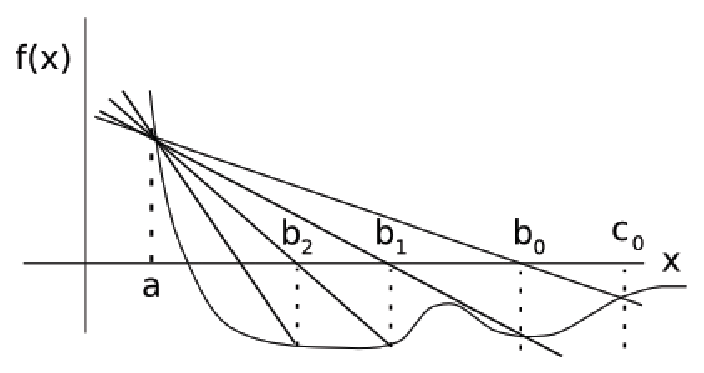
\includegraphics[scale=0.8]{capitulos/capitulo1/figuras/posicaofalsa2.eps}
  \caption{A seqüência de aproximações converge para $b$ por um único lado.}
  \label{fig:posicaofalsa2}
\end{figure}

\end{enumerate}

\subsection{Método da Posição Falsa Modificado}

Esse método elimina o problema de ponto estagnado. Cria-se um contador para verificar quantas vezes o ponto permaneceu um ponto de extremidade. Se o ponto permanecer ponto extremo por mais de duas vezes, divide-se o valor de $f$ (estagnado) por dois.

\begin{figure}[htb]
  %\index{figura da posição falsa modificado}%
  \setlength{\abovecaptionskip}{20pt}
  %%% o valor default de \abovecaptionskip definido para a classe
  %%% article e de 10pt.
  \centering
  %%% VIDE ABAIXO COMENTARIO SOBRE USO DE DIRETORIOS NO PATHNAME
  %%% DOS ARQUIVOS INCLUIDOS.
  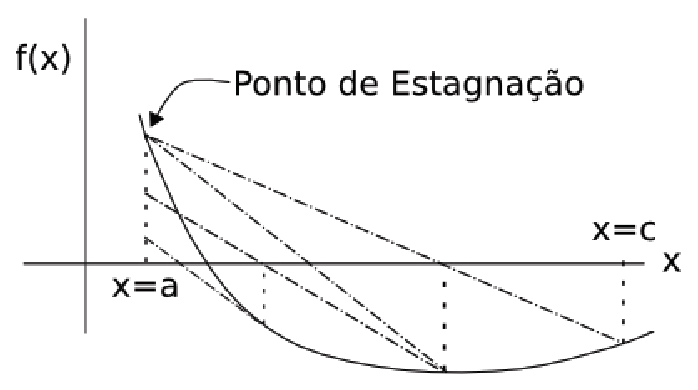
\includegraphics[scale=0.8]{capitulos/capitulo1/figuras/posicaofalsamodificado1.eps}
  \caption{Eliminando o problema do ponto de estagnação.}
  \label{fig:posicaofalsamodificado1}
\end{figure}

\begin{example}
 Usando o método da posição falsa, encontre a menor raíz positiva de $f(x) = \tan(x) - x - 0.5 = 0$, com $\xi = 0.00001$. Sabendo-se que ela se encontra em $ 0.1 < x < 1.4$.

\begin{table}[htp]
\footnotesize
	\centering
		
		\begin{tabular}{|c|c|c|c|c|c|c|}
		\hline		
		\textbf{Iteração} & \textbf{a} & \textbf{b} & \textbf{c} & \textbf{f(a)} & \textbf{f(b)} & \textbf{f(c)}\\
		\hline \hline 
		0 & 0.01 & 0.24771 & 1.4 & -0.49967 & -0.49481 & 3.8979\\
		\hline 
		1 & 0.24771 & 0.48102 & 1.4 & -0.49481 & -0.45911 & 1.9489\\
		\hline 
		2 & 0.48102 & 0.77533 & 1.4 & -0.45911 & -0.29527 & 0.97447\\
		\hline 
		3 & 0.77533 & 1.0110 & 1.4 & -0.29527 & 0.084850 & 0.48724\\
		\hline 
		4 & 0.77533 & 0.95842 & 1.0110 & -0.29527 & -0.034845 & 0.084850\\
		\hline 
		5 & 0.95842 & 0.97374 & 1.0110 & -0.034845 & -0.0027664 & 0.084850\\
		\hline  
		6 & 0.97374 & 0.97603 & 1.0110 & -0.0027664 & 0.0021981 & 0.042425\\
		\hline 
		7 & 0.97374 & 0.97501 & 0.97603 & -0.0027664 & -0.0000061 & 0.0021981\\
		\hline
		8 & 0.97501 & 0.97502 & 0.97603 & -0.0000061 & 0.0000000 & 0.0021981\\
		\hline
		\end{tabular}
	%\caption{Iterações do método da bisseção}
	\caption{Exemplo de iterações do método da posição falsa modificado.}
	\label{tab:posicaofalsamodificado}
\end{table}

$\xi_{_{MAX}} = 0.97603 - 0.97502 = 0.00101$

$\xi = 0.97502 - 0.97501 = 0.00001$

\end{example}

%%% Secao 4
\section{Método de Newton}
%\index{Método de Newton}

\subsection{Características}

\begin{itemize}
 \item Necessita uma aproximação inicial da raíz desejada.
 \item Usa a reta tangente calculada analiticamente.
 \item Pode ser aplicado para o cálculo de raízes complexas.
 \item Derivado a partir da expansão de Taylor.
\end{itemize}

\subsection{Descrição do Método}

\begin{equation}
 \label{eq:newton1}
 f(x) = 0 = f(x_{0} + f'(x_{0}) \ast (x - x_{0})) + O(h^{2})
\end{equation}

\[
 \displaystyle \left( \frac{f^{(n)}(x_{0})}{n!} \ast h^{n} \right)
\]

onde $h = x - x_{0}$.

Desprezando $O(h^{2})$ e resolvendo \ref{eq:newton1}, temos:

\begin{equation}
 \label{eq:newton2}
 x = x_{0} - \frac{f(x_{0})}{f'(x_{0})}
\end{equation}

Devido ao erro de truncamento, $x$ encontrado em \ref{eq:newton2} não é a solução de \ref{eq:newton1}, mas é uma melhor aproximação do que $x_{0}$.

\begin{figure}[htb]
  %\index{figura da posição falsa modificado}%
  \setlength{\abovecaptionskip}{20pt}
  %%% o valor default de \abovecaptionskip definido para a classe
  %%% article e de 10pt.
  \centering
  %%% VIDE ABAIXO COMENTARIO SOBRE USO DE DIRETORIOS NO PATHNAME
  %%% DOS ARQUIVOS INCLUIDOS.
  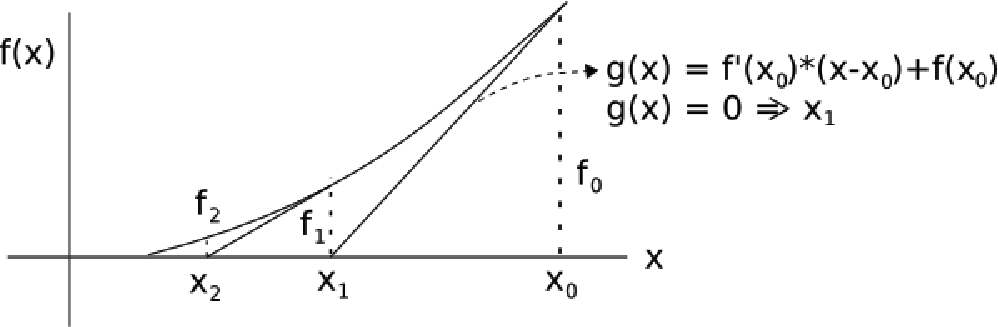
\includegraphics[scale=0.8]{capitulos/capitulo1/figuras/newton1-eps-converted-to.pdf}
  \caption{Ilustração para o método de Newton.}
  \label{fig:newton1}
\end{figure}

\[\displaystyle x_{i} = x_{i-1} - \frac{f(x_{i-1})}{f'(x_{i-1})}\]

\textbf{Notas:}

\begin{enumerar}
 \item O cálculo de $f'(x)$ pode ser difícil ou impossível. Nesses casos utiliza-se aproximação por diferenças finitas:

 \begin{itemize}
  \item \textit{Forward} $\displaystyle \rightarrow f'(x_{i-1}) \approx \frac{f(x_{i-1} + h) - f(x_{i-1})}{h} \, $ onde $h$ é um valor pequeno.

  \item \textit{Backward} $\displaystyle \rightarrow f'(x_{i-1}) \approx \frac{f(x_{i-1}) - f(x_{i-1} - h)}{h}$
 \end{itemize}

 \item Pequenos erros no cálculo de $f'(x_{i-1})$ não afetam muito a taxa de convergência.

 \item Se $f(x)$ não tem ponto de singularidade na vizinhança da raiz, as duas aproximações por diferenças finitas funcionam bem.

 \item Este método é de primeira ordem porque utiliza a primeira derivada.

 \item Métodos de segunda ordem teriam uma convergência mais rápida, mas o cálculo de derivada segunda, geralmente, elimina a vantagem sobre o método de primeira ordem.

\end{enumerar}

\begin{example}
 Derive um esquema iterativo baseado no método de Newton para encontrar a raiz cúbica de um número. Encontre a raiz de 155.

 \textbf{Solução:}

\[
\sqrt[3]{a} = x \Rightarrow x^{3} = a \Rightarrow f(x) = x^{3} - a
\]
 
Aplique o método de Newton

\[
 x_{n+1} = x_{n} - \frac{f(x_{n})}{f'(x_{n})} = x_{n} - \frac{x_{n}^{3} - a}{3 \ast x_{n}^{2}}
\]

\[
 x_{n+1} = \frac{2}{3} \ast x_{n} + \frac{a}{3 \ast x_{n}^{2}}
\]

Cálculo de $\sqrt[3]{155} \Rightarrow a = 155$.

\begin{enumerar}
\item Estimativa inicial $x_{0} = 5$:

\begin{table}[htp]
\footnotesize
	\centering
		
		\begin{tabular}{|c|c|c|}
		\hline		
		\textbf{$n$} & \textbf{$x$} & \textbf{$\displaystyle | x_{n+1} - x_{n} |$}\\
		\hline \hline 
		0 & 5 & -\\
		\hline 
		1 & 5.4 & 0.4\\
		\hline 
		2 & 5.371834 & 0.028\\
		\hline 
		3 & \underline{5.371685} & 0.00014\\
		\hline
		\end{tabular}
	%\caption{Iterações do método da bisseção}
	\caption{Exemplo de iterações do método de Newton para $x_{0} = 5$.}
	\label{tab:newton1}
\end{table}

\item Estimativa inicial $x_{0} = 10$:

\begin{table}[htp]
\footnotesize
	\centering
		
		\begin{tabular}{|c|c|c|}
		\hline		
		\textbf{$n$} & \textbf{$x$} & \textbf{$\displaystyle | x_{n+1} - x_{n} |$}\\
		\hline \hline 
		0 & 10 & -\\
		\hline 
		1 & 7.183334 & 2.816666\\
		\hline 
		2 & 5.790176 & 1.393158\\
		\hline
		3 & 5.401203 & 0.388973\\
		\hline
		4 & 5.371847 & 0.029383\\
		\hline
		5 & \underline{5.371686} & 0.000161\\
		\hline
		\end{tabular}
	%\caption{Iterações do método da bisseção}
	\caption{Exemplo de iterações do método de Newton para $x_{0} = 10$.}
	\label{tab:newton2}
\end{table}

\end{enumerar}

\end{example}

\begin{example}
\label{ex:newton1}

Encontre a primeira raiz positiva de $y = \tan(x) - 0.5 \ast x$ pelo método de Newton.

\textbf{Solução:}

\[
 y' = \frac{1}{\cos^{2}(x)} - 0.5 = \tan^{2}(x) + 0.5
\]

\[
 x_{n+1} = x_{n} - \frac{\tan(x_{n}) - 0.5 \ast x_{n}}{\tan^{2}(x_{n}) + 0.5}
\]

\begin{figure}[htb]
  %\index{figura da posição falsa modificado}%
  \setlength{\abovecaptionskip}{20pt}
  %%% o valor default de \abovecaptionskip definido para a classe
  %%% article e de 10pt.
  \centering
  %%% VIDE ABAIXO COMENTARIO SOBRE USO DE DIRETORIOS NO PATHNAME
  %%% DOS ARQUIVOS INCLUIDOS.
  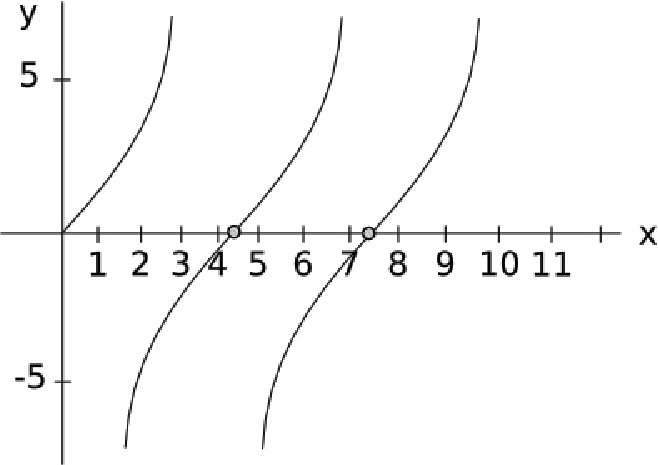
\includegraphics[scale=0.8]{capitulos/capitulo1/figuras/newton2-eps-converted-to.pdf}
  \caption{Ilustração para o método de Newton.}
  \label{fig:newton2}
\end{figure}

\begin{enumerar}
\item $\xi = 0.0001$

\item $x_{0} = 4$

\begin{table}[htp]
\footnotesize
	\centering		
		\begin{tabular}{|c|c|c|}
		\hline		
		\textbf{$n$} & \textbf{$x$} & \textbf{$\displaystyle | x_{n+1} - x_{n} |$}\\
		\hline \hline 
		0 & 4 & -\\
		\hline 
		1 & 4.458280 & 0.458280\\
		\hline 
		2 & 4.352068 & 0.106212\\
		\hline
		3 & 4.288511 & 0.033557\\
		\hline
		4 & 4.275191 & 0.013320\\
		\hline
		5 & 4.274782 & 0.000409\\
		\hline
		6 & \underline{4.244782} & 0.000000\\
		\hline
		\end{tabular}
	%\caption{Iterações do método da bisseção}
	\caption{Iterações do método de Newton para $x_{0} = 4$.}
	\label{tab:newton3}
\end{table}

\item $\xi = 0.0001$

$x_{0} = 3.6$

\begin{table}[htp]
\footnotesize
	\centering		
		\begin{tabular}{|c|c|c|}
		\hline		
		\textbf{$n$} & \textbf{$x$} & \textbf{$\displaystyle | x_{n+1} - x_{n} |$}\\
		\hline \hline 
		0 & 3.6 & -\\
		\hline 
		1 & 5.358891 & 1.758891\\
		\hline 
		2 & 7.131396 & 1.772505\\
		\hline
		3 & 8.494651 & 1.363255\\
		\hline
		4 & 10.92057 & 2.425919\\
		\hline
		5 & 10.87581 & 0.04476\\
		\hline
		6 & 10.83419 & 0.04162\\
		\hline
		7 & 10.81511 & 0.01908\\
		\hline
		8 & 10.81269 & 0.00242\\
		\hline
		9 & \underline{10.81267} & 0.00002\\
		\hline
		\end{tabular}
	%\caption{Iterações do método da bisseção}
	\caption{Iterações do método de Newton para $x_{0} = 3.6$.}
	\label{tab:newton4}
\end{table}

\end{enumerar}

\end{example}

\noindent
\textbf{OBS:}

\begin{itemize}
 \item O m\'etodo necessita de uma boa estimativa inicial, caso contr\'ario a solu\'c\~ao iterativa pode divergir ou convergir para uma solu\'c\~ao iterativa irrelevante.

 \item A taxa de converg\^encia elevada \`a  medida que se aproxima da solu\'c\~ao iterativa.
\end{itemize}

Suponha que $x$ seja a solução.

\begin{description}
\item[] $f(x) = f(x_{i}) + f'(x_{i}) \ast \xi_{i} + \displaystyle \frac{1}{2} \ast f''(x_{i}) \ast \xi_{i}^{2} + ... = 0$

\item[] $f'(x_{i}) = - f'(x_{i}) \ast \xi_{i} - \displaystyle \frac{1}{2} \ast f''(x_{i}) \ast \xi_{i}^{2}$

\item[] Método de Newton $\displaystyle \Rightarrow x_{i+1} = x_{i} - \frac{f(x_{i})}{f'(x_{i})} $

\item[] $\displaystyle x - x_{i+1} = x - x_{i} + \frac{f(x_{i})}{f'(x_{i})} \Rightarrow$

\item[] $\displaystyle  \Rightarrow \xi_{i+1} = \xi_{i} - \frac{f'(x_{i}) \ast \xi_{i}}{f'(x_{i})} - \frac{f''(x_{i}) \ast \xi_{i}^{2}}{2 \ast f'(x_{i})} \Rightarrow$

\item[] $\displaystyle \Rightarrow \xi_{i+1} = - \frac{f''(x_{i})}{2 \ast f'(x_{i})} \ast \xi_{i}^{2}$

\item[] $\displaystyle \xi_{i+1} = - \xi_{i}^{2} \ast \frac{f''(x)}{2 \ast f'(x)}$

\end{description}

%%% Secao 5
\section{Método da Secante}
%\index{Método da Secante}

\subsection{Características}

\begin{itemize}
\item Necessita de duas aproximações iniciais da raiz desejada
\item Usa a reta secante passando por dois valores de $f$ consecutivos no processo iterativo.
\end{itemize}

\subsection{Descrição}

\begin{figure}[htb]
  %\index{figura da posição falsa modificado}%
  \setlength{\abovecaptionskip}{20pt}
  %%% o valor default de \abovecaptionskip definido para a classe
  %%% article e de 10pt.
  \centering
  %%% VIDE ABAIXO COMENTARIO SOBRE USO DE DIRETORIOS NO PATHNAME
  %%% DOS ARQUIVOS INCLUIDOS.
  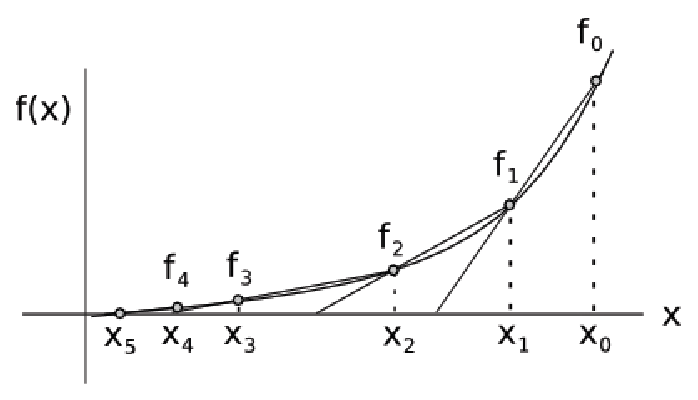
\includegraphics[scale=0.8]{capitulos/capitulo1/figuras/secante1.eps}
  \caption{Descrição do método da secante.}
  \label{fig:secante1}
\end{figure}

Considerando-se $h = x_{n-1} - x_{n-2}$ e utilizando-se \textit{backward} diferença finita para calcular $f'(x_{n-1})$ temos:

\[
 f'(x_{n-1}) = \frac{f(x_{n-1}) - f(x_{n-2})}{x_{n-1} - x_{n-2}}
\]

\[
 x_{n} = x_{n-1} - \frac{f(x_{n-1})}{f'(x_{n-1})} \approx x_{n-1} - \frac{f(x_{n-1})}{\frac{\displaystyle f(x_{n-1}) - f(x_{n-2})}{\displaystyle x_{n-1} - x_{n-2}}}
\]

\[
x_{n} = x_{n-1} - \frac{x_{n-1} - x_{n-2}}{f_{n-1} - f_{n-2}} \ast f_{n-1}
\]

\[
 n = 2, 3, ...
\]

%%% Secao 6
\section{Método das Substituições Sucessivas (Iteração de Ponto Fixo)}
%\index{Método das Substituições Sucessivas (Iteração de Ponto Fixo)}

\subsection{Descrição}

Dado $f(x) \Rightarrow f(x) = 0$ rearranja-se $f(x) = 0$ na forma:

\[
 x = \overline{f}(x)
\]

Assim, pode-se escrever um método iterativo como:

\[
 x_{i} = \overline{f}(x_{i-1})
\]

\subsection{Características}

\begin{itemize}
 \item Necessita de uma estimativa incial.
 \item Tem a vantagem de ser simples.
 \item Flexibilidade na escolha de $\overline{f}$.
 \item Para garantir convergência $\overline{f'}(x) < 1$ deve ser satisfeita na vizinhança da raiz.

\begin{itemize}
 \item $0 < \overline{f'} < 1 \Rightarrow$ convergência assintótica.
 \item $-1 < \overline{f'} < 0 \Rightarrow$ convergência oscilatória.
\end{itemize}

\end{itemize}

\begin{figure}[htb]
  %\index{figura da posição falsa modificado}%
  \setlength{\abovecaptionskip}{20pt}
  %%% o valor default de \abovecaptionskip definido para a classe
  %%% article e de 10pt.
  \centering
  %%% VIDE ABAIXO COMENTARIO SOBRE USO DE DIRETORIOS NO PATHNAME
  %%% DOS ARQUIVOS INCLUIDOS.
  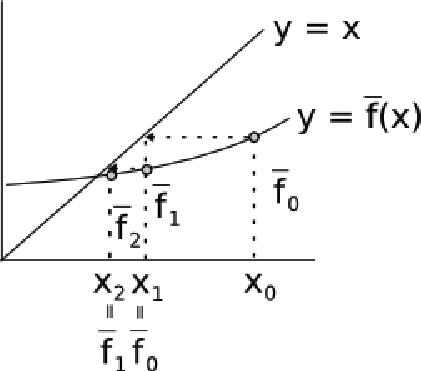
\includegraphics[scale=0.9]{capitulos/capitulo1/figuras/substituicoes1-eps-converted-to.pdf}
  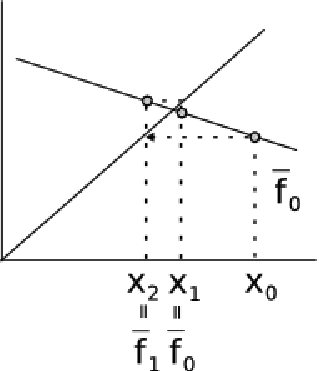
\includegraphics[scale=0.9]{capitulos/capitulo1/figuras/substituicoes2-eps-converted-to.pdf}
  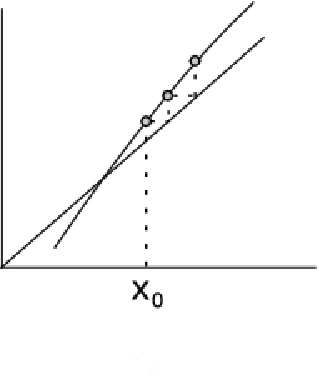
\includegraphics[scale=0.9]{capitulos/capitulo1/figuras/substituicoes3-eps-converted-to.pdf}
  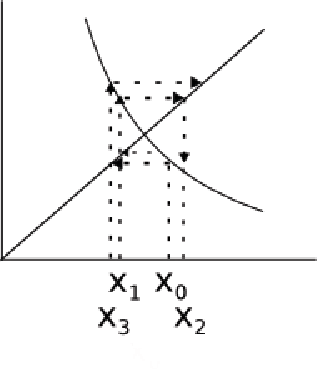
\includegraphics[scale=0.9]{capitulos/capitulo1/figuras/substituicoes4-eps-converted-to.pdf}

  \caption{Descrição do método das substituições sucessivas.}
  \label{fig:substituicoes1}  
\end{figure}

\subsection{Notas}

\begin{enumerar}
 \item Se $x_{n-2}$ e $x_{n-1}$ se tornarem muito próximos, $y_{n-2}$ e $y_{n-1}$ também se tornam próximos e erro de arredondamento significativo ocorre na divisão $ \displaystyle \frac{x_{n-1} - x_{n-2}}{f_{n-1} - f_{n-2}} $. Para evitar isso:

\begin{itemize}
 \item Quando $ |f_{n}| < \Delta$:

 \begin{enumerar}
 \item congela-se $x_{n-2}$ e $y_{n-2}$

 \item ou $x_{n-2}$ e $f_{n-2}$ são trocados por $x_{n-2} + \xi$ é $f(x_{n-2} + \xi)$ onde $\xi$ é pequeno mas suficientemente grande para evitar erro de arredondamento.
 \end{enumerar}

\end{itemize}

 \item O método pode divergir ou convergir para uma solução irrelevante se as aproximações iniciais não forem boas.

 \item O método é uma variação, computacionalmente mais eficiente, do método de Newton.

 \end{enumerar}

\begin{example}
\label{ex:substituicoes1}

 $f(x) = x^{2} - 3 \ast x + e^{x} - 2$ tem duas raízes, uma negativa e outra positiva. Encontre a menor raiz pelo método das substituições sucessivas.

\textbf{Solução:}

\begin{enumerate}

\item Tente determinar um intervalo que contém a raiz:

\begin{itemize}
 \item Para $x = 0 \Rightarrow f(0) = -1$.
 \item Para $x = -1 \Rightarrow f(-1) = 2.367$.
 \item Se $f(x)$ for contínua nesse intervalo a curva cortará o eixo dos $x$.
\end{itemize}

\item Reescreva $f(x) = 0$ na forma $x = \overline{f}(x)$:
\[
 x^{2} - 3 \ast x + e^{x} - 2 = 0 \Rightarrow x = \frac{x^{2} + e^{x} -2}{3}
\]

\item Método iterativo:

\[
 x_{i} = \frac{x_{i-1}^{2} + e^{x_{i-1}} -2}{3}
\]

onde $ \displaystyle \overline{f}(x) = \frac{x^{2} + e^{x} -2}{3}$

\item Verifique condição de convergência $|\overline{f'}(x) | < 1$

\[
 \overline{f'}(x) = \frac{1}{3} \ast (2 \ast x + e^{x})
\]
\[
 -1 < \frac{1}{3} \ast (2 \ast x + e^{x}) < 1
\]
\[
 \Rightarrow -3 < \frac{1}{3} \ast (2 \ast x + e^{x}) < 3
\]
\[
 \forall x \in [-1,0] \Rightarrow -1.63 \leq 2 \ast x + e^{x} \leq 1
\]

\underline{Conclusão:} O critério é convergente no intervalo.

\item Aplique o método iterativo com $x_{0} = 0$.

\begin{table}[htp]
\footnotesize
	\centering
		
		\begin{tabular}{|c|c|}
		\hline		
		\textbf{$n$} & \textbf{$x_{n}$}\\
		\hline \hline 
		0 & 0\\
		\hline 
		1 & -0.333333\\
		\hline 
		2 & -0.390786\\
		\hline 
		3 & -0.390254\\
		\hline
		4 & -0.390272\\
		\hline
		5 & -0.390272\\
		\hline
		\end{tabular}
	%\caption{Iterações do método da bisseção}
	\caption{Exemplo de iterações do Método das Substituições Sucessivas.}
	\label{tab:sucessivo1}
\end{table}

\underline{Resposta:} Solução de $f(x) = 0$

$x = -0390272$ (ver tabela \ref{tab:sucessivo1})

Outras opções para $\overline{f'}(x):$

\[
 x = - \sqrt{3 \ast x - e^{x} + 2}
\]

e

\[
 x = \sqrt{3 \ast x - e^{x} + 2}
\]

\[
 \overline{f'}(x) = \pm \frac{1}{2} \ast \frac{3 - e^{x}}{\sqrt{3 \ast x - e^{x} + 2}}
\]

Para $x = 0 \Rightarrow \overline{f'}(0) = \pm \frac{1}{2} \ast \frac{3 - 1}{\sqrt{1}} = \pm 1$
\[
 x= -1 \Rightarrow \overline{f'}(-1) = \pm \frac{1}{2} \ast \frac{1}{2} \ast \frac{3 - e^{-1}}{\sqrt{-3 - e^{-1} + 2}} = \pm \frac{1.32}{\sqrt{-1.37}}
\]

Critério de convergência não é satisfeito.

$\overline{f'}(x)$ é singular na vizinhança da raiz.

\end{enumerate}

\end{example}

\subsection{Forma sistemática de encontrar $\overline{f'}(x)$}

\[
 \bar{f}\,(x) = x - \alpha \, f \, (x) \Rightarrow \bar{f}\,(x) = 1 - \alpha \, f'\,(x)
\]

Assim, o esquema iterativo pode ser escrito como

\[
 \mbox{ \framebox{ $ x_n = x_{n-1} - \alpha \, f\,(x_{n-1}) $ } } \qquad (*)
\]

onde \esp{\alpha = constante}.

OBS: Se o esquema converge, \esp{x} satisfaz \esp{f(0) = 0}.

Critério de convergência:

\[
-1 < 1 - \alpha \, f'(x) < 1
\]

ou

\[
 \mbox{ \framebox{ $ 0 < \alpha \, f'(x) < 2 $ } } \qquad (**)
\]

\begin{itemize}
 \item \esp{\alpha} deve ter o mesmo sinal de \esp{f'(x)}
 \item para \esp{\alpha \approx 0 \Rightarrow} (*) sempre converge
 \item se \esp{\alpha \approx \displaystyle \frac{1}{f'(x)} \, \, * \underbrace{h}_{\mbox{\textit{\scriptsize{para cada iteração}}}}} , a convergência é ótima e o método se reduz ao método de Newton.
\end{itemize}

\begin{example}
Seja $f\,(x) = \tan\,(0.1\,x) - 9.2 \, e^{-x}$. Determine a menor raiz positiva sabendo-se que ela se encontra em \esp{[3,\,4]}

\textbf{Solução:}

\begin{itemize}
 \item Aproximação de $f'$ no intervalo \esp{[3,\,4]}:
 \esp{
  \begin{array}{ll}
   f' & = \displaystyle \frac{f\,(4) - f\,(3)}{4-3} = 0.40 \\
   \\
      & = 0.40299
  \end{array}
 }

 \item \esp{\alpha \approx \displaystyle \frac{1}{f'} = \frac{1}{0.40299} = 2.4814}

 \item \esp{x_n = x_{n-1} - 2.4814 \, [\tan\,(0.1\,x) - 9.2\,e^{-x}]}

\end{itemize}

\begin{table}[htp]
\footnotesize
	\centering
		
		\begin{tabular}{|c|c|}
		\hline		
		\textbf{$n$} & \textbf{$x_{n}$}\\
		\hline \hline 
		0 & 4\\
		\hline 
		1 & 3.36899\\
		\hline 
		2 & 3.28574\\
		\hline 
		3 & 3.29384\\
		\hline
		4 & 3.28280\\
		\hline
		5 & 3.29293\\
		\hline
		6 & 3.29292\\
		\hline
		7 & 3.29292\\
		\hline
		\end{tabular}
	%\caption{Iterações do método da bisseção}
	\caption{Exemplo de Forma sistemática de encontrar $\overline{f'}(x)$.}
	\label{tab:sucessivo2}
\end{table}

\[
 x = 3.29292
\]

\end{example}

\textbf{Nota:} O método de Newton e o método da Secante são casos particulares do método das substituições sucessivas.

%%% Secao 7
\section{Método de Bairstow}
%\index{Método de Bairstow}

\subsection{Características do método}

\begin{itemize}
 \item É um método especializado para determinação das raízes de um polinômio.
 \item O método apresenta problemas de precisão e não funciona sempre.
 \item É um método iterativo para o cálculo de um fator quadrático $P\,(x) = (x^2 + p\,x + q) \, G\,(x) + \underbrace{R\,(x)}_{0}$, $p$ e $q$ devem ser escolhidos para que o resto seja $0$.
 \item Aplicando-se o método repetidamente o polinômio original é ?deplacionado?.
\end{itemize}

\subsection{Descrição}

Qualquer polinômio

\begin{equation}
 \label{cap1:sec7:eq1}
 P\,(x) = a_0 + a_1 \, x_0 + a_2 \, x^2 + \ldots + a_n \, x^n
\end{equation}
 
Pode ser escrito na forma:

\begin{equation}
 \label{cap1:sec7:eq2}
 P\,(x) = (x^2 + p\,x + q) \, G\,(x) + R\,(x)
\end{equation}

onde:

\begin{itemize}
 \item \esp{p} e \esp{q} são arbitrários
 \item \esp{G\,(x)} é de ordem \esp{n-2}
 \item \esp{R\,(x)} é o resto (polinômio de ordem 1)
\end{itemize}

Se \esp{p} e \esp{q} são encontrados da forma que \esp{R\,(x) = 0}, então (\esp{x^2 + p\,x + q}) é um fator quadrático cujas raízes são \esp{x_{1}}, \esp{x_{2}} da solução de
\esp{
 \left.
 \begin{array}{l}
  x_1 \\
  x_2
 \end{array}
 \right\}
 =
 \frac{-p \sqrt{p^2 \pm 4\,q}}{2}
}.

\begin{equation}
 \label{cap1:sec7:eq3}
 G\,(x) = b_2 + b_3\,x + b_4\,x^2 + \ldots + b_{n-1}\,x^{n-3} + b_n\,x^{n-2}
\end{equation}

\begin{equation}
 \label{cap1:sec7:eq4}
 R\,(x) = b_0 + b_1\,x
\end{equation}

Como \esp{b_{0}} e \esp{b{1}} dependem de \esp{p} e \esp{q}, podemos escrever:

\begin{equation}
 \label{cap1:sec7:eq5}
 \begin{array}{l}
  b_{0} = b_{0}(p,q) \\
  b_{1} = b_{1}(p,q)
 \end{array}
\end{equation}

Problema: encontrar \esp{p = \overline{p}} e \esp{q = \overline{q}} tal que \esp{R(x) = 0}. \esp{R\,(x)} só pode ser nulo se:

\[
 \left.
 \begin{array}{l}
  b_{0}(p,q) = 0 \\
  b_{1}(p,q) = 0
 \end{array}
 \right\}
 \mbox{ Sistema de Equações}
\]

Resolução do sistema:

\[
 \left\{
 \begin{array}{l}
  b_{0} \, (p,\,q) = 0 \\
  b_{1} \, (p,\,q) = 0
 \end{array}
 \right.
\]

Pelo o método de Newton.
\\\\
\textbf{Solução:}
\\\\
Suponha que ($p$, $q$) seja uma aproximação da solução ($\overline{p}$, $\overline{q}$). A expansão de primeita ordem em série de Taylor

\[
 \left\{
 \begin{array}{l}
  b_0\,(\overline{p},\,\overline{q}) \approx b_0 \, (p,\,q) + \displaystyle \frac{\partial b_0}{\partial p} \, \Delta p + \frac{\partial b_0}{\partial q} \, \Delta q = 0 \\
  \\
  b_1\,(\overline{p},\,\overline{q}) \approx b_1 \, (p,\,q) + \displaystyle \frac{\partial b_1}{\partial p} \, \Delta p + \frac{\partial b_1}{\partial q} \, \Delta q = 0
 \end{array}
 \right.
\]

\esp{\Delta p = \overline{p} - p} e \esp{\Delta q = \overline{q} - q}

Assim,

\begin{equation}
 \label{cap1:sec7:eq8}
 \left\{
 \begin{array}{l}
  \displaystyle \frac{\partial b_0}{\partial p} \, \Delta p + \frac{\partial b_0}{\partial q} \, \Delta q = - b_0\,(p,\,q) \\
  \\
  \displaystyle \frac{\partial b_1}{\partial p} \, \Delta p + \frac{\partial b_1}{\partial q} \, \Delta q = - b_1\,(p,\,q)
 \end{array}
 \right.
\end{equation}

Derivação de uma forma explícita para o sistema

Eq. \ref{cap1:sec7:eq3} e \ref{cap1:sec7:eq4} \esp{\Rightarrow} \ref{cap1:sec7:eq2}

\begin{equation}
 \label{cap1:sec7:eq6}
 \begin{array}{l}
 \begin{array}{rrrrrrrrrrrrl}
         &   &           &   & b_2\,x^2 & + & b_3 \, x^3 & + & \ldots & + & b_{n-1}\,x^{n-1} & + & b_n\,x^n \\
         &   & p\,b_2\,x & + & p\,b_3\,x^2 & + & p\,b_4\,x^3 & + & \ldots & + & p\,b_n\,x^{n-1} & & \\
  q\,b_2 & + & q\,b_3\,x & + & q\,b_4\,x^2 & + & q\,b_5\,x^3 & + & \ldots & & & + & q\,b_n\,x^{n-2} \\
  b_0    & + & b_1\,x & & & & & & & & & & \\
 \end{array}
 +
 \\
 \overline{ (b_0 + q\,b_2) + (q\,b_3 + p\,b_2 + b_1)\,x + (b_2 + p\,b_3 + q\,b_4)\,x^2 + \ldots + (b_{n-2} + p\,b_{n-1} + q\,b_n)\,x^{n-2} + }\\
 (b_{n-1} + p\,b_n)\,x^{n-1} + b_n\,x^n = P\,(x)
 \end{array}
\end{equation}

Comparando-se \ref{cap1:sec7:eq6} com \ref{cap1:sec7:eq1}:

\begin{equation}
 \label{cap1:sec7:eq7}
 \left\{
 \begin{array}{cl}
  b_n     & = a_n \\
  b_{n-1} & = a_{n-1} - p\,b_n \\
  b_{n-2} & = a_{n-2} - p\,b_{n-1} - q\,b_n \\
  b_{n-3} & = a_{n-3} - p\,b_{n-2} - q\,b_{n-1} \\
  \vdots  & \\
  b_2     & = a_2 - p\,b_3 - q\,b_4 \\
  b_1     & = a_1 - p\,b_2 - q\,b_3
 \end{array}
 \right.
\end{equation}

Derivando \ref{cap1:sec7:eq7} com relação a \esp{p} temos

\begin{equation}
 \label{cap1:sec7:eq9}
 \left\{
 \begin{array}{cllll}
  (b_n)_p & = & 0 & & \\
  (b_{n-1})_p & = & -b_n & - p\,(b_n)_p & \\
  (b_{n-2})_p & = & -b_{n-1} & - p\,(b_{n-1})_p & - q\,(b_n)_p \\
  (b_{n-3})_p & = & -b_{n-2} & - p\,(b_{n-2})_p & - q\,(b_{n-1})_p \\
  \vdots  & \\
  (b_2)_p & = & -b_3 & - p\,(b_3)_p & - q\,(b_4)_p \\
  (b_1)_p & = & -b_2 & - p\,(b_2)_p & - q\,(b_3)_p \\
  (b_0)_p & = &      &              & - q\,(b_2)_p \\
 \end{array}
 \right.
\end{equation}

Derivando \ref{cap1:sec7:eq7} com relação a \esp{q} temos:

\begin{equation}
 \label{cap1:sec7:eq10}
 \left\{
 \begin{array}{cllll}
  (b_n)_q & = & 0 & & \\
  (b_{n-1})_q & = & 0 & & \\
  (b_{n-2})_q & = & -b_n & & \\
  (b_{n-3})_q & = & - p\,(b_{n-2})_q & - b_{n-1} & - q\,(b_{n-1})_q \\
  \vdots  & \\
  (b_2)_q & = & - p\,(b_3)_q & - b_4 & - q\,(b_4)_q \\
  (b_1)_q & = & - p\,(b_2)_q & - b_3 & - q\,(b_3)_q \\
  (b_0)_q & = &              & - b_2 & - q\,(b_2)_q \\
 \end{array}
 \right.
\end{equation}

\textbf{Implementação:}

\begin{enumerate}
\item Com estimativas iniciais de $p$ e $q$, calcule $b_{0}$ e $b_{1}$ utilizando equação \ref{cap1:sec7:eq7}
\label{implem:item:1}

\item Calcule $(b_{0})_{p}$, $(b_{1})_{p}$, $(b_{0})_{q}$ e $(b_{1})_{q}$ pelas equações \ref{cap1:sec7:eq9} e \ref{cap1:sec7:eq10}.
\label{implem:item:2}
OBS: Todas as equações em \ref{implem:item:1} e \ref{implem:item:2} são calculadas recursivamente.

\item Resolve o sistema \ref{cap1:sec7:eq8} para $\Delta p - \Delta q$.

\item Obtenha $\overline{p}$ e $\overline{q}$
\label{implem:item:4}

$\overline{p} = p + \Delta p$

$\overline{q} = q + \Delta q$

\end{enumerate}

O procedimento de \ref{implem:item:1} a \ref{implem:item:4}  é iterativo com novas estimativas de $\overline{p}$ e $\overline{q}$ a cada iteração.

\subsection{Notas}

\begin{itemize}
\item Com a aplicação repetida do método, o erro no cálculo dos polinômios ?defacionados? e dos fatores quadráticos.
\item A precisão das raízes pode ser pobre, assim a precisão deve ser melhorada por outro método.
\item A iteração pode não convergir em ?
\end{itemize}

%%% Capitulo 2
\chapter{Integração Numérica}

%%% Secao 1
\section{Introdução}
%\index{Introdução}%

A integral definida pode ser interpretada como a \'area da regi\~ao limitada pelo gr\'afico de uma fun\c{c}\~ao e o plano de refer\^encia (ou eixo) das vari\'aveis livres. 
Essa \'area tem sinal positivo se estiver acima do plano de refer\^encia, e, sinal negativo se estiver abaixo do plano de refer\^encia.

No caso de uma fun\c{c}\~ao de uma \'unica vari\'{a}vel, a integral definida no intervalo $[a, b]$ \'e representada por 

\begin{equation}
 I = \int_a^b \, f\,(x) \, dx
\end{equation}

\noindent
e indicada como a \'area entre o gr\'afico da fun\c{c}\~ao, $f(x)$, o eixo dos $x$ e as retas $x = a$ e $x = b$ (Figura \ref{fig:intro1}).

\begin{figure}[htb]
 \centering
    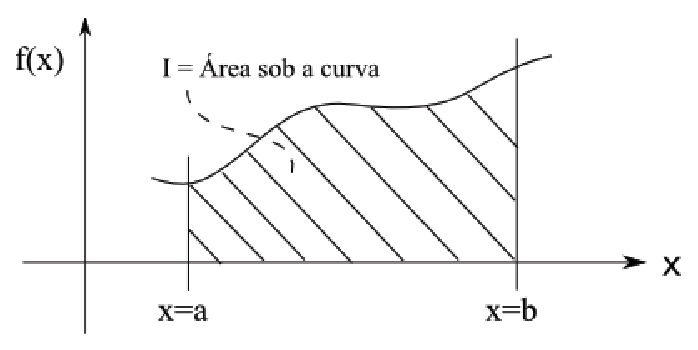
\includegraphics[scale=0.8]{capitulos/capitulo2/figuras/intro1.eps}
    \caption{\'Area sob a curva representando a integral}
    \label{fig:intro1}
\end{figure}

No caso de uma fun\c{c}\~ao de duas vari\'{a}veis, a integral definida em uma regi\~{a}o do plano \'e representada por

\begin{equation}
   I = \displaystyle \int_a^b \, \int_{u\,(x)}^{v\,(x)} \, f\,(x,\,y) \, dy \, dx
\end{equation}

\noindent
e indicada como o volume entre o gr\'afico da fun\c{c}\~ao, $f(x,y)$, o plano $xy$, os planos $x = a$ e $x = b$ e as superf\'icies $y = u(x)$ e $y = v(x)$ (Figura \ref{fig:intro2}).

\begin{figure}[htb]
 \centering
    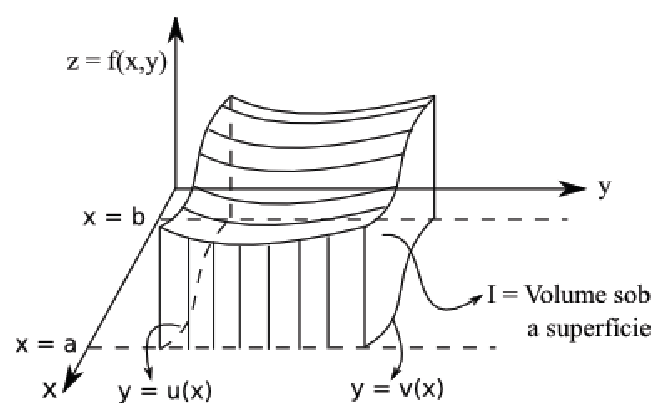
\includegraphics[scale=0.8]{capitulos/capitulo2/figuras/intro2.eps}
    \caption{Volume sob a superfície representando a integral}
    \label{fig:intro2}
\end{figure}

A integra\c{c}\~ao num\'erica pode ser usada tanto para integrar fun\c{c}\~oes anal\'iticas, quanto para integrar fun\c{c}\~oes apresentadas em forma tabular, quando se deseja o valor num\'erico da integral.

\paragraph{Filosofia geral dos m\'etodos de integra\c{c}\~ao}

A filosofia geral dos m\'etodos de integra\c{c}\~ao \'e substituir o integrando por uma fun\c{c}\~ao polinomial que aproxime o gr\'afico da fun\c{c}\~ao a ser integrada. Essa id\'eia est\'a representada na equa\c{c}\~ao \ref{eq:filosofia_geral}

\begin{equation}
   I = \int_a^b \, f\,(x) \, dx \approx \int_a^b \, g\,(x) \, dx
   \label{eq:filosofia_geral}
\end{equation}

\noindent
onde $g(x)$ \'e o polin\^omio de substitui\c{c}\~ao de grau adequadamente escolhido.



%%% Secao 2
\section{Regra do Trapézio}

\begin{figure}[htb]
 \centering
\begin{minipage}[c]{7cm}
    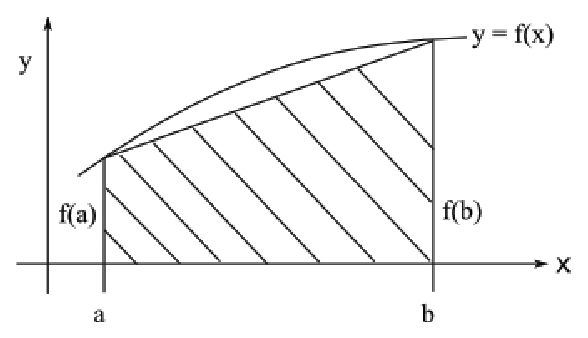
\includegraphics[scale=0.8]{capitulos/capitulo2/figuras/regra_trapezio1.eps}
    \caption{Área sob a reta representando a integral}
    \label{fig:regra_trapezio1}
 \end{minipage}\hspace*{1cm}
 \begin{minipage}[c]{6cm}
    \begin{equation}
     \label{cap2:sec2:eq1}
     I = \int_a^b \, f\,(x) \, dx = \frac{b - a}{2} \, [f\,(a) + f\,(b)] + E
    \end{equation}

    onde \esp{E = \mbox{erro}}.
 \end{minipage}
\end{figure}

\subsection{Erro da Regra do Trapézio}

\[
 E = \int_a^b \, f\,(x) \, dx - \frac{b - a}{2} \, [f\,(a) + f\,(b)]
\]

Expansão de Taylor de \esp{f(x)} na vizinhança de \esp{\overline{x} = \frac{a + b}{2}}

\[
 f\,(x) = f\,(\overline{x}) + \frac{f'(\overline{x})}{1!} \, (x - \overline{x}) + \frac{f''(\overline{x})}{2!} \, (x - \overline{x})^2 + \ldots
\]

Assim,

\begin{equation}
 \label{cap2:sec2:eqA}
 \begin{array}{ll}
  \displaystyle \int_a^b f\,(x) \, dx & = f\,(\overline{x}) \left. \, x \, \right|_a^b + f'(\overline{x}) \, \left\{ \left. \displaystyle \frac{x^2}{2} \, \right|_a^b - \overline{x} \left. \, x \, \right|_a^b \right\} + \displaystyle \frac{f''(\overline{x})}{2} \left\{ \left. \frac{x^3}{3} \, \right|_a^b - \overline{x} \left. \, x^2 \, \right|_a^b \, \overline{x}^{\,2} \left. \, x \, \right|_a^b \right\} \\
                        & = f\,(\overline{x}) \, (b - a) + f'(\overline{x}) \, \left\{ \displaystyle \frac{(b - a)}{1} \, \underbrace{\frac{(b + a)}{2}}_{\overline{x}} - \overline{x} \, (b - a) \right\} + \\
                        & + \displaystyle \frac{f''(\overline{x})}{2} \, \left\{ \frac{b^3 - a^3}{3} - \overline{x} \, (b^2 - a^2) + \overline{x}^{\,2} \, (b - a) \right\} \\
                        & = f\,(\overline{x}) \, (b - a) + \displaystyle \frac{1}{24} \, f''(\overline{x}) \, (b - a)^3 + \ldots
 \end{array}
\end{equation}

\begin{equation}
 \label{cap2:sec2:eqB}
 \begin{array}{ll}
  \displaystyle \frac{b - a}{2} \, [f\,(a) + f\,(b)] & = \displaystyle \frac{b - a}{2} \, \left\{ f\,(\overline{x}) + f'(\overline{x}) \left[ \underbrace{a - \frac{a + b}{2}}_{-\frac{1}{2}\,(b - a)} \right] + \frac{1}{2}\,f''(\overline{x}) \left[ \underbrace{a - \frac{a + b}{2}}_{-\frac{1}{2}\,(b - a)} \right]^2 + \ldots \right. \\
  \\
  & \left. + f\,(\overline{x}) + f'(\overline{x}) \, \left[ \underbrace{b - \frac{a + b}{2}}_{\frac{1}{2} \, (b - a)} \right] + \frac{1}{2} \, f''(\overline{x}) \, \left[ \underbrace{b - \frac{a + b}{2}}_{\frac{1}{2} \, (b - a)} \right]^2 \, \right\} \\
  \\
  & = \displaystyle \frac{b - a}{2} \, \left\{ 2\,f\,(\overline{x}) + f''(\overline{x}) \, \frac{1}{4} \, (b - a)^2 + \ldots \right\} \\
  & = f\,(\overline{x}) \, (b - a) + \displaystyle \frac{1}{8} \, f''(\overline{x}) \, (b - a)^3 + \ldots
 \end{array}
\end{equation}

\[
 \begin{array}{ll}
  & E \approx f''(\overline{x}) \, (b - a)^3 \, \left(\displaystyle \frac{1}{24} - \frac{1}{8}\right) \approx - \displaystyle \frac{1}{12} \, f''(\overline{x}) \, (b - a)^3 \\
  \\
  (\ref{cap2:sec2:eqA}) & \mbox{ \framebox{ $ E \approx - \displaystyle \frac{1}{12} \, f''(\overline{x}) \, h^3 $ } }
 \end{array}
\]

Se \esp{h = \displaystyle \frac{b - a}{N}}, então

\[
 \begin{array}{ll}
  (\ref{cap2:sec2:eqB}) & \mbox{ \framebox{ $ E \approx - \displaystyle \frac{1}{12} \, \frac{(b - a)^3}{N^3} \, \sum_{i=1}^N \, f''(\overline{x}_i) $ } } \\
  \\
  & \mbox{ \framebox{ $ E \approx - \displaystyle \frac{1}{12} \, (b - a) \, h^2 \, \overline{f}\,'' $ } }
 \end{array}
\]

onde

\[
 \overline{f}\,'' = \sum_{i=1}^N \, \frac{f''(\overline{x}_i)}{N}
\]

\subsection{Múltiplos Intervalos}

\begin{itemize}
 \item $n$ = número de intervalos = número de trapézios
\item $h$ = altura dos trapézios = \esp{\displaystyle \frac{b - a}{n}}
\end{itemize}

\begin{figure}[htb]
 \centering
 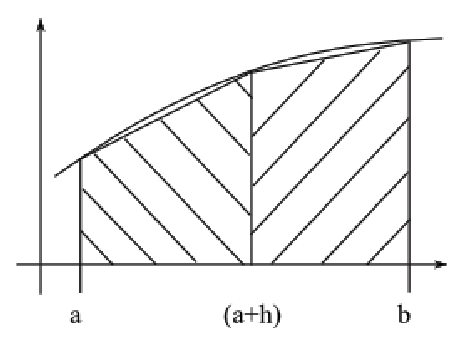
\includegraphics[scale=0.8]{capitulos/capitulo2/figuras/regra_trapezio2.eps}
 \caption{Área sob a reta representando a integral com intervalos}
 \label{fig:regra_trapezio2}
\end{figure}

Suponha:

\[
 \begin{array}{ll}
  n = 2 \Rightarrow I & = \displaystyle \frac{1}{2} \left[ f\,(a) + f\,(a + h) \right] \, h + \frac{1}{2} \left[ f\,(a + h) + f\,(b) \right] \, h \vspace*{0.2cm} \\
                      & = \displaystyle \frac{h}{2} \, \left[ f\,(a) + 2\,f\,(a + h) + f\,(b) \right] \\
  \\
  n = 3 \Rightarrow I & = \displaystyle \frac{1}{2} \left[ f\,(a) + f\,(a + h) \right] \, h + \frac{1}{2} \left[ f\,(a + h) + f\,(a + 2\,h) \right] \, h + \frac{1}{2} \, \left[ f\,(a + 2\,h) + f\,(b) \right] \, h \vspace*{0.2cm} \\
                      & = \displaystyle \frac{h}{2} \, \left\{ f\,(a) + 2\,\left[ f\,(a + h) + f\,(a + 2\,h) + f\,(a + 3\,h) \right] + f\,(b) \right\} \\
  \\
  n = 4 \Rightarrow I & = \displaystyle \frac{h}{2} \left\{ f\,(a) + 2\,\left[ f\,(a + h) + f\,(a + 2\,h) + f\,(a + 3\,h) \right] + f\,(b) \right\}
 \end{array}
\]

\begin{equation}
 \begin{array}{l}
  n = N \Rightarrow \mbox{ \framebox{ $ I = \displaystyle \frac{h}{2} \left\{ f\,(a) + 2\,\sum_{i=1}^{N-1} \, f\,(a + i\,h) + f\,(b) \right\} $ } }
 \end{array}
\end{equation}

\begin{example}

\begin{figure}[htb]
 \centering
 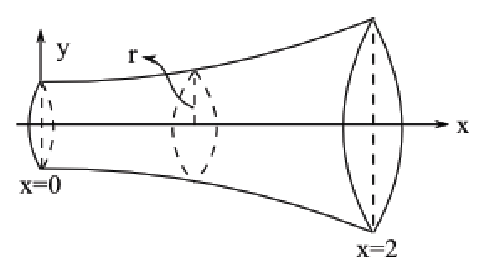
\includegraphics[scale=1.0]{capitulos/capitulo2/figuras/regra_trapezio3.eps}
 \caption{Volume de superfície curva}
 \label{fig:regra_trapezio2}
\end{figure}

\[
 \overline{f}\,(x) = 1 + \left( \frac{x}{2} \right)^2, \, \, 0 \leq x \leq 2
\]

Calcule o volume

\[
 \begin{array}{ll}
  V & = \displaystyle \int_0^2 \pi \, r^2 \, dx = \int_0^2 \pi \, \left[ 1 + \frac{x^2}{4} \right]^2 \, dx = \int_0^2 \pi \, \left( 1 + \frac{x^2}{2} + \frac{x^4}{16} \right) \, dx \\
    & = \left. \pi \, \left[ x + \displaystyle \frac{x^3}{6} + \frac{x^5}{80} \right] \displaystyle \, \right|_0^2 = \pi \, \left(2 + \displaystyle \frac{2^3}{6} + \frac{2^5}{80}\right) = 11.7286 \\
    & ?
 \end{array}
\]

\end{example}

%%% Secao 3
\section{Regra $\frac{1}{3}$ de Simpson}

\begin{enumerate}
 \item Polinômio interpolante:

\[
 \begin{array}{ll}
  g\,(x_0 + s\,h) & = \displaystyle \left(s \atop 0\right) \, \Delta^0 \, f_0 + \left(s \atop 1\right) \, \Delta^1 \, f_1 + \left(s \atop 2\right) \, \Delta^2 \, f_2 \\
  g\,(x_0 + s\,h) & = 1 \, f_0 + s\,(f_1 - f_0) + \displaystyle \frac{1}{2} \, s \, (s - 1) \, (f_2 - 2\,f_1 + f_0)
 \end{array}
\]

\[
 \quadricular{ g\,(x_0 + s\,h) = f_0 + (f_1 - f_0)\,s + \displaystyle \frac{1}{2} \, (f_2 - 2\,f_1 + f_0) \, (s^2 - s) }
\]

\item Integrando o polinômio quadrático, temos:

\[
 I = \int_{x_0}^{x_2} g\,(x) \, dx
 \qquad
 \begin{array}{rcl}
  x & = & x_0 + h\,s \qquad 
  \left\{
  \begin{array}{l}
   x = x_0 \rightarrow s = 0 \\
   x = x_2 \rightarrow s = 2
  \end{array}
  \right.
  \\
  dx & = & h\,ds
 \end{array}
\]

\[
 \begin{array}{ll}
  I & = \displaystyle \int_0^2 g\,(x_0 + s\,h) \, \, h \, \, ds \\
    & = \left. h \, \left[ f_0\,s + (f_1 - f_0) \, \displaystyle \frac{s^2}{2} + \frac{1}{2} \, (f_2 - 2\,f_1 + f_0)\,\left(\frac{s^3}{3} - \frac{s^2}{2}\right) \right] \, \right|_0^2 \\
    & = h \, \left[ 2\,f_0 + (f_1 - f_0) \, \displaystyle \frac{4}{2} + \frac{1}{2} \, (f_2 - 2\,f_1 + f_0) \, \left( \underbrace{\frac{8}{3} - \frac{8}{4}}_{\frac{16 - 12}{6} = \frac{4}{6} = \frac{2}{3}} \right) \right] \\
    & = h \, \left[ 2\,f_0 + 2\,f_1 - 2\,f_0 + \displaystyle \frac{1}{3}\,f_2 - \frac{2}{3}\,f_1 + \frac{1}{3}\,f_0 \right] \\
    & = \displaystyle \frac{h}{3} \, \left[ f_0 + 4\,f_1 + f_2 \right]
 \end{array}
\]


\end{enumerate}

\subsection{Erros das Regras de Simpson}

\begin{itemize}

\item $ \displaystyle \frac{1}{3}$ Simpson: \esp{E \approx - \displaystyle \frac{h^5}{90} \, f^{(IV)}(\overline{x})}

\textbf{OBS:} Se $f(x)$ for polinômio de grau $\leq 3$ então \esp{f^{(IV)}(\overline{x}) = 0} e consequentemente o erro é zero.

\item Regra $ \displaystyle \frac{1}{3}$ de Simpson estendida:

\[
 E \approx - (b - a) \, \frac{h^4}{180} \, \overline{f}^{(IV)}
\]

onde: 

\[
 \overline{f}^{\,(IV)} = \sum_{i=1}^{N/2} \frac{f^{(IV)}(\overline{x}_i)}{(N/2)}
\]

\item $ \displaystyle \frac{3}{8}$ Simpson: \esp{ - \displaystyle \frac{3}{80} \, h^5 \, f^{(IV)}(\overline{x}) }

\item Regra $ \displaystyle \frac{3}{8}$ de Simpson estendida: \esp{ E \approx - \displaystyle \frac{3}{240} \, (b-a) \, h^4 \, \overline{f}^{\,(IV)} }

\end{itemize}



%%% Secao 4
\section{Integração de Romberg}

Suponha que $I_{n}$ seja o resultado da integração pela regra do trapézio estendida com \esp{k = \displaystyle \frac{(b-a)}{N}}

Suponha que $I_{2n}$ seja o resultado para \esp{ \overline{h} = \displaystyle \frac{(b-a)}{(N/2)} }.

Assim,

\begin{equation}
 \label{cap2:sec4:eq1}
 E_h \approx - \frac{1}{12} \, (b-a) \, \overline{f}'' \, h^2 \approx C\,h^2
\end{equation}

\begin{equation}
 \label{cap2:sec4:eq2}
 E_{2\,h} \approx - \frac{1}{12} \, (b-a) \, \overline{f}'' \, (2\,h)^2 \approx 4\,C\,h^2
\end{equation}

A integral exata é

\begin{equation}
 \label{cap2:sec4:eq3}
I = I_h + E_h = I_{2\,h} + E_{2\,h}
\end{equation}

Assim,

\begin{equation}
 \label{cap2:sec4:eq4}
 E_h - E_{2\,h} = I_{2\,h} - I_h
\end{equation}

Eq. \ref{cap2:sec4:eq1} e \ref{cap2:sec4:eq2} $ \rightarrow $ \ref{cap2:sec4:eq4} $ \Rightarrow $

\[
 \begin{array}{ll}
              & C\,h^2 - 4\,C\,h^2 = I_{2\,h} - I_h \\
  \Rightarrow & C = \displaystyle \frac{1}{3} \, h^{-2} \, (I_h - I_{2\,h})
 \end{array}
\]

\[
 E_h \approx \frac{1}{3} \, (I_h - I_{2\,h})
\]

\[
 \quadricular{ I = I_h + E_h \approx I_h + \frac{1}{3} \, (I_h - I_{2\,h}) }
\]

\begin{example}

\[
 \begin{array}{ll}
  I_{0.5} = 11.9895 \qquad \qquad & I_{0.25} = 11.7940 \\
  \uparrow & \uparrow \\
  N = 2 & N = 4 \\
  \\
  h = 0.25
 \end{array}
\]

\[
 \begin{array}{lc}
  I = 11.7940 + \displaystyle \frac{1}{3} \, (11.7940 - 11.9895) & \approx 11.7288 \\
  & \uparrow \\
  & \approx I_{0.0156} \\
  & \uparrow \\
  & N = 128
 \end{array}
\]

\end{example}

%%% Secao 5
\section{Fórmulas de Newton-Cotes}

Os métodos de integração derivados a partir da integração das fórmulas de interpolação de Newton são as fórmulas de integração de Newton-Cotes.

\begin{enumerate}
 \item

As fórmulas fechadas de Newton-Cotes são aquelas onde as extremidades do intervalo de integração são utilizados como pontos amostrais.

\[
 \int_a^b f\,(x) \, dx = \alpha \, h \, \left[ w_0\,f_0 + w_1\,f_1 + w_2\,f_2 + \ldots + w_n\,f_n \right] + E
\]

onde $\alpha$ e $w$ são constantes e

\[
 f_i = f\,(x_i)\,, \qquad x_i = a + i\,h\,, \qquad h = \frac{(b-a)}{N}
\]

{
\footnotesize
\begin{center}
\begin{tabular}{|c|c|c|c|}
	\hline		
	\textbf{N} & \textbf{$\alpha$} & \textbf{$w_i\,,\,i=0\,,\,\ldots\,,\,N$} & \textbf{E} \\
	\hline \hline
	1 & 1/2 & 1 1 & $- \displaystyle \frac{1}{12} \, h^3 \, f''$ \\
	\hline 
	2 & 1/3 & 1 4 1 & $- \displaystyle \frac{1}{90} \, h^5 \, f^{(iv)}$ \\
	\hline 
	3 & 3/8 & 1 3 3 1 & $- \displaystyle \frac{3}{80} \, h^5 \, f^{(iv)}$ \\
	\hline 
	4 & 2/45 & 7 32 12 32 7 & $- \displaystyle \frac{8}{945} \, h^7 \, f^{(vi)}$ \\
	\hline 
\end{tabular}
\end{center}
\label{cap2:sec5:tab1}
}

\item

As fórmulas abertas são aquelas que os limites de integração inferior e superior estão distantes $h$ do primeiro ponto e do último ponto. Por exemplo, para $n = 1$ (trapézio).

\begin{figure}[htb]
 \centering
 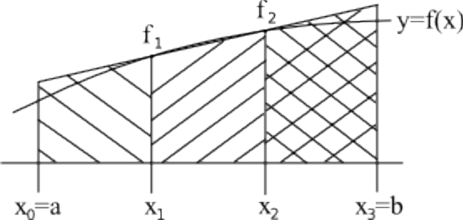
\includegraphics[scale=1.0]{capitulos/capitulo2/figuras/formula_newton_cotes1.pdf}
 \caption{Exemplo para $N = 1$ (trapézio)}
 \label{fig:formula_newton_cotes1}
\end{figure}

\[
 \int_a^b f\,(x) \, dx = \alpha \, h \, \left[ w_0\,f_0 + w_1\,f_1 + \dots + w_{n+2}\,f_{n+2} \right] + E
\]

\begin{table}[htp]
\footnotesize
	\centering
		
		\begin{tabular}{|c|c|c|c|}
		\hline		
		\textbf{N} & \textbf{$\alpha$} & \textbf{$w_i\,,\,i=0\,,\,\ldots\,,\,N+2$} & \textbf{E} \\
		\hline \hline
		1 & 3/2 & 0 1 1 0 & $- \displaystyle \frac{1}{4} \, h^3 \, f''$ \\
		\hline 
		2 & 4/3 & 0 2 -1 2 0 & $- \displaystyle \frac{28}{90} \, h^5 \, f^{(iv)}$ \\
		\hline 
		3 & 5/24 & 0 11 1 1 11 0 & $- \displaystyle \frac{95}{144} \, h^5 \, f^{(iv)}$ \\
		\hline 
		4 & 6/20 & 0 11 -14 26 -14 11 0 & $- \displaystyle \frac{41}{140} \, h^7 \, f^{(vi)}$ \\
		\hline 
		\end{tabular}
	\caption{Fórmulas abertas de Newton-Cotes.}
	\label{cap2:sec5:tab1}
\end{table}

\end{enumerate}

\begin{example}

\esp{N = 1}

\begin{figure}[htb]
 \centering
 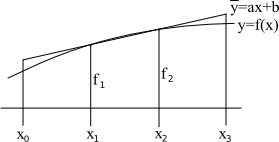
\includegraphics[scale=1.0]{capitulos/capitulo2/figuras/formula_newton_cotes2.png}
 \caption{Outro exemplo para $N = 1$ (trapézio)}
 \label{fig:formula_newton_cotes2}
\end{figure}

\[
 \begin{array}{ll}
  I = \mbox{ área do trapézio } & = \displaystyle \frac{1}{2} \, (f_0 + f_3) \, 3\,h = \frac{1}{2} \, (f_1 + f_2) \, 3\,h \\ \\
                                & = \displaystyle \frac{3}{2} \, h \, [0 \, f_0 + 1 \, f_1 + 1 \, f_2 + 0 \, f_3]
 \end{array}
\]

\[
 N = 2 \rightarrow g\,(x_1 + s\,h) = f_1 + (f_2 - f_1) \, s + \frac{1}{2} \, (f_3 - 2\,f_2 + f_1)\,(s^2 - s)
\]

\[
\begin{array}{l}
 \begin{array}{l}
  x = x_1 + h\,s \\
  x = x_0 \rightarrow s = -1 \\
  x = x_4 \rightarrow s = 3
 \end{array}
 \qquad
 \begin{array}{ll}
  \displaystyle \int_{x_0}^{x_4} g\,(x) \, dx & = \displaystyle \int_{-1}^3 g\,(x_1 + s\,h) \, h\,ds \\
                                & = \displaystyle \frac{4}{3} \, h \left\{ 0\,f_0 + 2\,f_1 - 1\,f_2 + 2\,f_3 + 0\,f_4 \right\}
 \end{array}
\end{array}
\]

\end{example}

\begin{example}
 Deducão de fórmula de newton-cotes de grau 4.

Temos que:

\emph{\[
I=\int_{a}^{b}{\scriptstyle f(x)dx}=\int_{a}^{b}{\scriptstyle g(x)dx}+E\]
}

De acordo com a regra de interpolacão de Newton 2.4.6 (pág 37 do livro
Applied Numerical methods in C, Nakamura), temos que a formula que
passar pelos K+1 pontos amostrais, $f_{0},f_{1},f_{2}...f_{k}$é dada
pela fórmula:

\[
g({\scriptstyle x})=g({\scriptstyle x_{0}+sh})=\sum_{n=0}^{k}{\scriptstyle \left(_{n}^{s}\right)\triangle^{n}f_{0}}\]


Então, podemos dizer que x está em funcão de s da seguinte forma:

\[
x\left(s\right)=x_{0}+sh\]


\[
dx=h.ds\]


Substituindo e aplicando n=4, temos:

\[
I=\int_{a}^{b}{\scriptstyle g(x)dx}=\int_{0}^{4}{\scriptstyle g(x(s))h.ds}=h\int_{0}^{4}{\scriptstyle g(x_{0}+sh)ds}\]


Sendo que:

\[
g(x)=g(x_{0}+sh)=\sum_{n=0}^{k}{\scriptstyle \left(_{n}^{s}\right)\triangle^{n}f_{0}}\]


Então desenvolvendo o somatório acima, teremos:

\[
g(x_{0}+sh)=g_{0}+s(g_{1}-g_{0})+\frac{s(s-1)}{2}(g{}_{2}-g{}_{1}+g_{0})+\frac{s^{3}-3s^{2}+2s}{6}(g_{3}-3g_{2}+3g_{1}-g_{0})\]


\[
+\frac{s(s-1)(s-2)(s-3)}{24}(g_{4}-4g_{3}+6g_{2}-4g_{1}+g_{0})\]


Substituindo na integral:

\[
h\int_{0}^{4}{\scriptstyle g_{0}+s(g_{1}-g_{0})+\frac{s(s-1)}{2}(g{}_{2}-g{}_{1}+g_{0})+\frac{s^{3}-3s^{2}+2s}{6}(g_{3}-3g_{2}+3g_{1}-g_{0})+\frac{s(s-1)(s-2)(s-3)}{24}(g_{4}-4g_{3}+6g_{2}-4g_{1}+g_{0})}\]


Integrando e isolando por$g_{k}$, temos:

\[
I\equiv h(\frac{14}{45}g_{0}+\frac{64}{45}g_{1}+\frac{24}{45}g_{2}+\frac{64}{45}g_{3}+\frac{14}{45}g_{4})\]


\[
I\equiv\frac{2h}{45}(7g_{0}+32g_{1}+12g_{2}+32g_{3}+7g_{4})_{\blacksquare}\]
\end{example}



%%% Secao 6
\section{Quadraturas de Gauss}

\subsection{Quadraturas de Gauss-Legendre}

\begin{enumerate}

\item 
OBS:

\begin{enumerate}

\item 
S\~ao m\'etodos num\'ericos de integra\'c\~ao que utilizam os pontos de Legendre (ra\'izes dos polin\^omios de Legendre)

\item
Apropriadas para fun\'c\~oes anal\'iticas.

\item
Precis\~ao muito maior do que as f\'ormulas de Newton-Cotes.

\item
Os pontos de Legendre \textbf{não são regularmente espaçados.}

\end{enumerate}

\item

\begin{enumerate}

 \item 
Erro da Regra do Trap\'ezio \'e proporcional a $f''$. Assim, se $f(x)$ for polin\^omio at\'e ordem 1, o erro \'e nulo.

\item
Erro da Regra do Trapézio é proporcional a $f^{IV}$. Assim, integra exatamente polinômios de até ordem 3.

\item
As fórmulas de Newton-Cotes com $n$ ímpar integram exatamente polinômios de ordem $n$ e as com $n$ par integram exatamente polinômios de ordem $n+1$.

\item
Vamos tentar uma fórmula de integração com dois pontos que integre exatamente um polinômio de ordem 3 (3 pontos [N-Cotes $n=2$] ou 4 pontos [N-Cotes $n=3$]).

\end{enumerate}

\begin{equation}
 \label{cap2:sec6:eq1}
 I = \int_{-1}^1 f\,(x) \, dx = w_1 \, f\,(x_1) + w_2 \, f\,(x_2) + E
\end{equation}

Queremos $E=0$ para $f(x)=1$, $f(x)=x$, $f(x)=x^{2}$ e $f(x)=x^{3}$.

Assim,

\begin{equation}
 \label{cap2:sec6:eq2}
 \begin{array}{llr}
  \int_{-1}^1 1 \, dx & = 2 = w_1 + w_2 \qquad & (a) \\
  \int_{-1}^1 x \, dx & = 0 = w_1\,x_1 + w_2\,x_2 \qquad & (b) \\
  \int_{-1}^1 x^2 \, dx & = \displaystyle \frac{2}{3} = w_1\,x_1^2 + w_2\,x_2^2 \qquad & (c) \\
  \int_{-1}^1 x^3 \, dx & = 0 = w_1\,x_1^3 + w_2\,x_2^3 \qquad & (d)
 \end{array}
\end{equation}

os limites de integração são simétricos em relação a $x=?$.

Assim, façamos $x_{1}$ e $x_{2}$ simétricos em relação a $x=0$

\[x_{2} = -x_{1}\]

\[
 \begin{array}{l}
  (\ref{cap2:sec6:eq2}.b) \Rightarrow w_1\,x_1 - w_2\,x_1 = x_1\,(w_1 - w_2) = 0 \\
  (\ref{cap2:sec6:eq2}.a) \Rightarrow w_1 + w_2 = 2 \neq 0 \Rightarrow w_1 = w_2 = 1
 \end{array}
\]

Com estes valores (\ref{cap2:sec6:eq2}.d) fica automaticamente satisfeita

\[
 0 = 1\,x_1^3 + 1\,(-x_1)^3 = x_1^3 - x_1^3
\]

\[
 \begin{array}{l}
  (\ref{cap2:sec6:eq2}.c) \Rightarrow \displaystyle \frac{2}{3} = x_1^2 + (-x_1)^2 = 2\,x_1^2 \Rightarrow x_1^2 = \frac{1}{3} \\ \\
  \qquad x_1 = \displaystyle \frac{1}{\sqrt{3}} \vspace*{0.2cm} \\
  \qquad x_2 = - \displaystyle \frac{1}{\sqrt{3}}
 \end{array}
\]


Para $n$ pontos de integração $x_{1}$, $x_{2}$, ... $x_{n}$ são as raízes do polinômio de Legendre de ordem $n$.

\[
 \quadricular{\displaystyle \int_{-1}^1 f\,(x) \, dx \approx \sum_{k=1}^N w_k \, f\,(x_k)}
\]

Polinômio de Legendre de ordem $n$.

\[
 P_n\,(x) = \frac{1}{2^N\,N!} \, \frac{d^N\,(x^2 - 1)^N}{dx^N}
\]

\[
 \begin{array}{l}
  P_0\,(x) = \displaystyle \frac{1}{2^0\,0!} \, (x^2 - 1)^0 = 1 \vspace*{0.2cm} \\
  P_1\,(x) = \displaystyle \frac{1}{2^1\,1!} \, \frac{d}{dx} \, (x^2 - 1)^1 = x \vspace*{0.2cm} \\
  P_2\,(x) = \displaystyle \frac{1}{2^2\,2!} \, \frac{d^2}{dx^2} \, (x^2 - 1)^2 = \frac{1}{2}\,(3\,x^2 - 1)
 \end{array}
\]

\begin{table}[htp]
\footnotesize
	\centering
		
		\begin{tabular}{|ccc|}
		\hline		
		& \textbf{$\pm \, x_i$} & \textbf{$w_i$} \\
		\hline \hline
		N=2 & $\pm$ 0.577350269 & 1.0 \\
		\hline 
		N=3 &
		$
		\left\{
		\begin{array}{l}
		 0 \\
		 \pm 0.774596669
		\end{array}
		\right.
		$
		&
		$
		\begin{array}{l}
		 0.888888889 = 8/9 \\
		 0.555555556 = 5/9
		\end{array}
		$
		\\
		\hline 
		N=4 &
		$
		\left\{
		\begin{array}{l}
		 \pm 0.339981043 \\
		 \pm 0.861136312
		\end{array}
		\right.
		$
		&
		$
		\begin{array}{l}
		 0.652145155 \\
		 0.347854845
		\end{array}
		$
		\\
		\hline
		\vdots & \vdots & \vdots \\
		\hline
		\end{tabular}
	%\caption{}
	\label{cap2:sec5:tab1}
\end{table}

\[
 \begin{array}{ll}
  I & = \displaystyle \int_a^b \, f\,(x) \, dx = \\ \\
    & = \displaystyle \frac{b-a}{2} \, \int_{-1}^1 \bar{f}\,(\xi) \, d\xi \\ \\
    & = \displaystyle \frac{b-a}{2} \, \sum_{k=1}^N \, w_k \, \bar{f}\,(\xi_k)
 \end{array}
\]

\begin{figure}[htb]
 \centering
 \begin{minipage}[c]{7cm}
    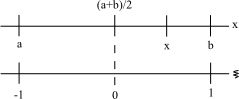
\includegraphics[scale=0.8]{capitulos/capitulo2/figuras/quadraturas_de_gauss1.png}
    \caption{Parametrização}
    \label{fig:quadraturas_de_gauss1}
 \end{minipage}\hspace*{1cm}
 \begin{minipage}[c]{6cm}
     \[
      \begin{array}{ll}
       x & = \displaystyle \frac{a+b}{2} + \xi \, \left(\frac{b-a}{2}\right) \\
       dx & = \displaystyle \frac{b-a}{2} \, d\xi
      \end{array}
     \]
 \end{minipage}
\end{figure}

\begin{example}
\[
 I = \int_0^2 \, \pi \, [1 + (x/2)^2]^2 \, dx
\]

\[
 \begin{array}{lll}
 \left.
 \begin{array}{l}
  b = 2 \\
  a = 0
 \end{array}
 \right\}
 & x & = \displaystyle \frac{0+2}{2} + \displaystyle \frac{2-0}{2} \, \xi = 1 + \xi \Rightarrow x = 1 + \xi \\
 & dx & = d\xi
 \end{array}
\]

$n=2$ integra exatamente $2n-1 = 4-1 = 3$

$n=3$ integra exatamente polinômio de grau $\leq$ 5.

Como o integrando é polinômio de grau 4 utilizaremos $n=3$

\[
\begin{array}{l}
 \xi_1 = - 0.774596669 \rightarrow f_1 = \pi \, \left\{ 1 + \left[ (1+\xi_1)/2 \right]^2 \right\}^2 = 3.2219064 \qquad w_1=5/9 \\
 ?
\end{array}
\]

\[
\begin{array}{ll}
 I & = \displaystyle \frac{5}{9} \, 3.2219064 + \frac{8}{9} \, 4.9087385 + \frac{5}{9} \, 10.0356146 \\
   & = 11.7286
\end{array}
\]

\end{example}

\item
Provar que, se $f(x)$ for um polinômio de ordem $2n-1$ ou menor, a quadratura de Gauss de ordem $n$ é exata.

\textbf{Prova:} Suponha que $f(x)$ em \esp{\int_{-1}^1 \, f\,(x) \, dx} seja um polinômio de ordem $2n-1$. Assim,

\begin{equation}
 \label{cap2:sec6:eq1}
 f\,(x) = c\,(x) \, P_N\,(x) + r\,(x)
\end{equation}

onde $P_{n}(x)$ é o polinômio de Legendre de ordem $n-1$

\begin{equation}
 \label{cap2:sec6:eq2}
 \int_{-1}^1 \, f\,(x)\,dx = \underbrace{\int_{-1}^1 \, c\,(x)\,P_N\,(x)\,dx}_{
  \begin{array}{l}
   \mbox{\footnotesize{$= 0$, pois o polinômio $P_N$}} \\
   \mbox{\footnotesize{é ortogonal a todos os}} \\
   \mbox{\footnotesize{polinômios de ordem $< N-1$}}
  \end{array}
 } + \int_{-1}^1 \, r\,(x)\,dx
\end{equation}

\begin{equation}
 \underbrace{
 \quadricular{
 \label{cap2:sec6:eq3}
 \int_{-1}^1 \, P_m \, (x) \, dx =
 \left\{
  \begin{array}{cl}
   0 & \qquad \mbox{para } n \neq m \\ \\
   \displaystyle \frac{2}{2\,n+1} & \qquad \mbox{para } m = n
  \end{array}
 \right.
 }
 }_{
  \mbox{\footnotesize{ortogonalidade dos polinômios de Legendre}}
 }
\end{equation}

\begin{equation}
 \label{cap2:sec6:eq4}
 \int_{-1}^1 \, f\,(x) \, dx = \int_{-1}^1 \, r\,(x) \, dx 
\end{equation}

Se $x_{i}$ é uma das raízes do polinômio de Legendre $P_{n}$, então:

\begin{equation}
 \label{cap2:sec6:eq5}
 f\,(x_i) = \underbrace{c\,(x_i) \, P_n\,(x_i)}_{0} + \, r\,(x_i) \Rightarrow f\,(x_i) = r\,(x_i)
\end{equation}

O polinômio \esp{r\,(x)} de ordem \esp{N-1} pode ser expresso exatamente pela interpolação de Lagrange de ordem \esp{N-1} (precisa de \esp{N} pontos amostrais)

\begin{equation}
 \label{cap2:sec6:eq6}
 r\,(x) =
 \sum_{i=1}^N \left[
  \prod_{
    j=1 \,\, j \neq i
  }^N
  \frac{x-x_j}{x_i-x_j}
 \right]
 r\,(x_i)
\end{equation}

\begin{example}

\begin{figure}[htb]
 \centering
 \begin{minipage}[c]{7cm}
    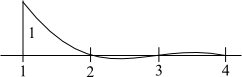
\includegraphics[scale=0.9]{capitulos/capitulo2/figuras/quadraturas_de_gauss2.png}
    \caption{?}
    \label{fig:quadraturas_de_gauss2}
 \end{minipage}\hspace*{1cm}
 \begin{minipage}[c]{6cm}
    \[
     r_1 \, \frac{x-x_2}{x_1-x_2} \, \frac{x-x_3}{x_1-x_3} \, \frac{x-x_4}{x_1-x_4}
    \]
 \end{minipage}
\end{figure}

\begin{figure}[htb]
 \centering
 \begin{minipage}[c]{7cm}
    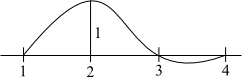
\includegraphics[scale=0.9]{capitulos/capitulo2/figuras/quadraturas_de_gauss3.png}
    \caption{?}
    \label{fig:quadraturas_de_gauss3}
 \end{minipage}\hspace*{1cm}
 \begin{minipage}[c]{6cm}
    \[
     r_2 \, \frac{x-x_1}{x_2-x_1} \, \frac{x-x_3}{x_2-x_3} \, \frac{x-x_4}{x_2-x_4}
    \]
 \end{minipage}
\end{figure}

\begin{figure}[htb]
 \centering
 \begin{minipage}[c]{7cm}
    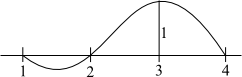
\includegraphics[scale=0.9]{capitulos/capitulo2/figuras/quadraturas_de_gauss4.png}
    \caption{?}
    \label{fig:quadraturas_de_gauss4}
 \end{minipage}\hspace*{1cm}
 \begin{minipage}[c]{6cm}
    \[
     r_3 \, \frac{x-x_1}{x_3-x_1} \, \frac{x-x_2}{x_3-x_2} \, \frac{x-x_4}{x_3-x_4}
    \]
 \end{minipage}
\end{figure}

\begin{figure}[htb]
 \centering
 \begin{minipage}[c]{7cm}
    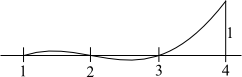
\includegraphics[scale=0.9]{capitulos/capitulo2/figuras/quadraturas_de_gauss5.png}
    \caption{?}
    \label{fig:quadraturas_de_gauss5}
 \end{minipage}\hspace*{1cm}
 \begin{minipage}[c]{6cm}
    \[
     r_4 \, \frac{x-x_1}{x_4-x_1} \, \frac{x-x_2}{x_4-x_2} \, \frac{x-x_3}{x_4-x_3}
    \]
 \end{minipage}
\end{figure}

\end{example}

Se os pontos amostrais forem as \esp{N} raízes de \esp{P_N\,(x)}, então, pela equação \ref{cap2:sec6:eq5}

\begin{equation}
 \label{cap2:sec6:eq7}
 r\,(x) =
 \sum_{i=1}^N \left[
  \prod_{
    j=1 \,\, j \neq i
  }^N
  \frac{x-x_j}{x_i-x_j}
 \right]
 f\,(x_i)
\end{equation}

Assim \ref{cap2:sec6:eq7} $\rightarrow$ \ref{cap2:sec6:eq4} $\Rightarrow$

\[
 \int_{-1}^1 \, f\,(x) \, dx = \int_{-1}^1 \, r\,(x) \, dx = \sum_{i=1}^N \, f\,(x_i) \,
 \underbrace{
 \int_{-1}^1 \left[
  \prod_{
    j=1 \,\, j \neq i
  }^N
  \frac{x-x_j}{x_i-x_j}
 \right]
 \, dx
 }_{
  w_i
 }
\]
\begin{example}
 \emph{ Deducao de Quadraturas de Gauss-legendre } 

-

-

A quadratura de Gauss-legendre é dada pela fórmula (4.6.1, na página
135 do livro Applied Numerical methods, Nakamura)

Temos que:

\emph{\[
\int_{-1}^{1}{\scriptstyle f(x)dx}\backsimeq\sum_{{\scriptstyle {\scriptscriptstyle k=1}}}^{{\scriptscriptstyle N}}{\scriptstyle w_{k}f(x_{k})}\]
}

Onde$x_{1},x_{2},x_{3}...x_{n}$ é dado pelas raizes de $P_{N}(x)=0$,$P_{N}(x)$
é o Polinomio de Legendre de ordem N. Tal polinomio é dado pela seguinte
fórmula(Appendix B, página 559 do livro Applied Numerical Methods,
Nakamura): \[
P_{4}(x)=\frac{1}{2^{4}4!}\frac{d^{4}(x^{2}-1)^{4}}{dx^{4}}\]


Onde, 

\[
\frac{1}{2^{4}4!}=\frac{1}{384}\]


logo, teremos:

\[
\frac{1}{384}\frac{d^{4}(x^{2}-1)^{4}}{dx^{4}}=\frac{1}{384}\frac{d^{4}}{dx^{4}}(x^{8}-4x^{6}+6x^{4}-4x^{2}+1)=\frac{1}{8}(35x^{4}-30x^{2}+3)\]


Para tirarmos as raízes, temos que:

\[
P_{4}(x)=0\]


Então,

\[
(35x^{4}-30x^{2}+3)=0\]


Tirando as raízes:

%\lyxline{\normalsize}

$x^{2}=a$ ,então a fórmula se tornará , $35a^{2}-30a+3=0$, daqui
é fácil ver que as raízes de a são: $a_{1}=\frac{15+2\sqrt{30}}{35}$
e $a_{2}=\frac{15-2\sqrt{30}}{35}$ .

como $x^{2}=a$ , teremos: $x_{1}=\sqrt{\frac{15+2\sqrt{30}}{35}};x_{2}=-\sqrt{\frac{15+2\sqrt{30}}{35}};x_{3}=\sqrt{\frac{15-2\sqrt{30}}{35}};x_{4}=-\sqrt{\frac{15-2\sqrt{30}}{35}};$

Teremos, então, $x_{1}=0,861136312;x_{2}=-0,861136312;x_{3}=0,339981043;x_{4}=-0,339981043;$

%\lyxline{\normalsize}

Como os pontos devem ser localizados simetricamente, temos que: $w_{1}=w_{2}$e$w_{3}=w_{4}.$

O cálculo de w é dado pela fórmula(página 138, do livro Applied Numerical
methods, Nakamura):

\[
w_{i}=\int_{-1}^{1}\left[\prod_{{\scriptscriptstyle j=1;j\neq i}}^{{\scriptscriptstyle N}}{\scriptstyle \frac{{\scriptstyle x-x_{j}}}{x_{i}-x_{j}}}\right]dx\]


Para $w_{1}$, teremos:

\[
w_{1}=\int_{-1}^{1}\left[\prod_{{\scriptscriptstyle j=1;j\neq i}}^{{\scriptscriptstyle N}}{\scriptstyle \frac{{\scriptstyle x-x_{j}}}{x_{i}-x_{j}}}\right]dx=\int_{-1}^{1}\left[\frac{(x-x_{2})(x-x_{3})(x-x_{4})}{(x_{1}-x_{2})(x_{1}-x_{3})(x_{1}-x_{4})}\right]dx\]


Integrando, temos:

\[
w_{1}=w_{2}=0,347854845\]


E para $w_{3}$, teremos:

\[
w_{3}=\int_{-1}^{1}\left[\prod_{{\scriptscriptstyle j=1;j\neq i}}^{{\scriptscriptstyle N}}{\scriptstyle \frac{{\scriptstyle x-x_{j}}}{x_{i}-x_{j}}}\right]dx=\int_{-1}^{1}\left[\frac{(x-x_{1})(x-x_{2})(x-x_{4})}{(x_{3}-x_{1})(x_{3}-x_{2})(x_{3}-x_{4})}\right]dx\]


Após integrar, teremos:

Temos, então:

\[
w_{3}=w_{4}=0,652145155\]


Substituindo os resultados, na fórmula da quadratura de Gauss-legendre
aplicada a N=4, teremos:

\[
\int_{-1}^{1}{\scriptstyle f(x)dx}\backsimeq0,347854845f(0,861136312)+0,347854845f(-0,861136312)\]


\[
+0,652145155f(0,339981043)+0,652145155f(-0,339981043)_{\blacksquare}\]
\end{example}


\subsection{Outras Quadraturas de Gauss}

\begin{enumerate}

\item 
\textbf{Gauss-Hermite}: apropriadas para integrais da forma

\[
 I = \int_{-\infty}^\infty \, e^{-x^2} \, f\,(x) \, dx \approx \sum_{k=1}^N \, w_k \, f\,(x_k)
\]

{
%\begin{table}[htp]
\footnotesize
	\begin{center}
		\begin{tabular}{|c|c|c|}
		\hline		
		\textbf{N} & \textbf{Pontos de Hermite: $\pm \, x_i$} & \textbf{Pesos de Hermite: $w_i$} \\
		\hline \hline
		2 & $\pm 0.70710678$ & $0.88622692$ \\
		\hline
		3 & $0.00000000$     & $1.18163590$ \\
		  & $\pm 1.22474487$ & $0.29540897$ \\
		\hline
		4 & $\pm 0.52464762$ & $0.80491409$ \\
		  & $\pm 1.65068012$ & $0.08131283$ \\
		\hline
		5 & $    0.00000000$ & $0.94530872$ \\
		  & $\pm 0.95857246$ & $0.39361932$ \\
		  & $\pm 2.02018287$ & $0.01995324$ \\
		\hline
		\end{tabular}
	\end{center}
	\label{cap2:sec6:tab2}
%\end{table}
}

\item
\textbf{Gauss-Laguerre}: apropriadas para integrais da forma

\[
 I = \int_0^\infty \, e^{-x} \, f\,(x) \, dx \approx \sum_{k=1}^N \, w_k \, f\,(x_k)
\]

{
%\begin{table}[htp]
\footnotesize
	\begin{center}
		\begin{tabular}{|c|c|c|}
		\hline		
		\textbf{N} & \textbf{Pontos de Laguerre: $x_i$} & \textbf{Pesos de Laguerre: $w_i$} \\
		\hline \hline
		2 & $0.58578643$ & $0.85355339$ \\
		  & $3.41421356$ & $0.14644660$ \\
		\hline
		3 & $0.41577455$ & $0.71109300$ \\
		  & $2.24428036$ & $0.27851973$ \\
		  & $6.28994508$ & $0.01038926$ \\
		\hline
		4 & $0.32254768$ & $0.60315410$ \\
		  & $1.74576110$ & $0.35741869$ \\
		  & $4.53662029$ & $0.03888791$ \\
		  & $9.39507091$ & $0.00053929$ \\
		\hline
		\end{tabular}
	\end{center}
	\label{cap2:sec6:tab3}
%\end{table}
}

\item
\textbf{Gauss-Chebyshev}: apropriadas para integrais da forma

\[
 I = \int_{-1}^1 \, \frac{1}{\sqrt{1-x^2}} \, f\,(x) \, dx \approx \sum_{k=1}^N \, w_k \, f\,(x_k)
\]

onde \esp{x_k = \cos\,\frac{k-1/2}{N} \, \pi}, \esp{k=1, 2, \ldots, N}

\[
 w_k = \frac{\pi}{N} \qquad \forall k
\]

Assim,

\[
 I = \int_{-1}^1 \, \frac{1}{\sqrt{1-x^2}} \, f\,(x) \, dx \approx \frac{\pi}{N} \, \sum_{k=1}^N \, f\,(x_k)
\]

\end{enumerate}

\end{enumerate}

\textbf{Nota}: todas as três quadraturas serão exatas se $f(x)$ for um polinômio de ordem $\leq 2n-1$ 

%%% Secao 7
\section{Roteiro da Aula}

\begin{enumerate}

\item
Falar sobre produto escalar de dois vetores:

\[
 \vec A \, \cdot \vec B = |\vec A| \, |\vec B| \, \cos \theta
\]

\begin{figure}[htb]
    \centering
    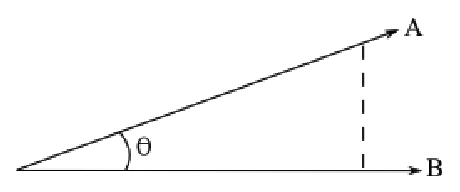
\includegraphics[scale=0.8]{capitulos/capitulo2/figuras/roteiro_da_aula1.eps}
    \caption{Produto escalar}
    \label{fig:roteiro_da_aula1}
\end{figure}

\[
 \vec A \, \cdot \vec B = \sum_{i=1}^N A_i \, B_i
\]

Se

\[
   \begin{array}{ll}
     \vec A \, \cdot \vec B = 0 & \Rightarrow \cos \theta = 0 \\
                                & \Rightarrow \theta = \displaystyle \frac{\pi}{2} + n\,\pi\,; \qquad n = 0, 1, \ldots \\
   \end{array}
\]

\begin{figure}[htb]
 \centering
 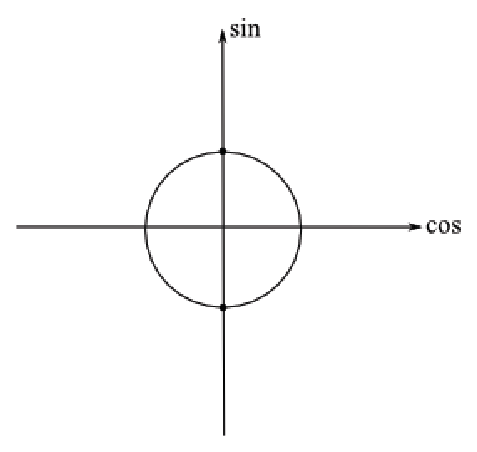
\includegraphics[scale=0.8]{capitulos/capitulo2/figuras/roteiro_da_aula2.eps}
 \caption{?}
 \label{fig:roteiro_da_aula2}
\end{figure}

dizemos que $\vec A$ e $\vec B$ são ortogonais.

\item
Estender a noção de ortogonalidade para funções

\begin{figure}[htb]
 \centering
 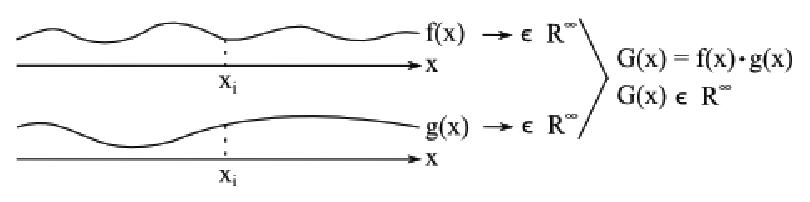
\includegraphics[scale=1.0]{capitulos/capitulo2/figuras/roteiro_da_aula3.eps}
 \caption{?}
 \label{fig:roteiro_da_aula3}
\end{figure}

\[
 \sum_i \, f\,(x_i) \, g\,(x_i) \equiv \sum_i \, G\,(x) \rightarrow \int \, f\,(x) \, g\,(x) \, dx = 0
\]

Se \esp{\int \, f\,(x) \, g\,(x) \, dx = 0} então $f(x)$ e $g(x)$ são ortogonais.

\item
Base de vetores ortogonais e polinômios ortogonais como base do espaço de polinômios. Mostrar que se um polinômio $P_{x}$ é ortogonal aos polinômios da base, então ele é perpendicular a todos os polinômios do espaço.

\begin{figure}[htb]
 \centering
 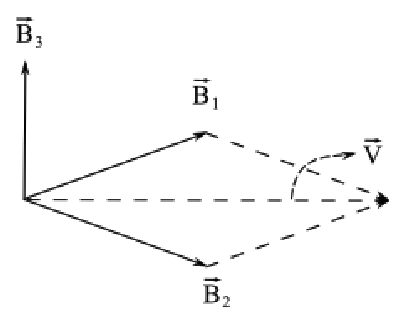
\includegraphics[scale=0.8]{capitulos/capitulo2/figuras/roteiro_da_aula4.eps}
 \caption{?}
 \label{fig:roteiro_da_aula4}
\end{figure}

\[
 \vec V = C_1 \, \vec B_1 + C_2 \, \vec B_2
\]

\[
 \left.
 \begin{array}{l}
  \vec B_3 \cdot \vec B_1 = 0 \\
  \vec B_3 \cdot \vec B_2 = 0
 \end{array}
 \right\}
 \Rightarrow
 \vec B_3 \cdot \vec V = 0
\]

\item
Mostrar a propriedade de ortogonalidade dos polinômios de Legendre

\[
 \int_{-1}^1 P_m\,(x) \, P_n\,(x)\,dx =
 \left\{
 \begin{array}{cl}
  0                & \qquad \mbox{para $n \neq m$} \\ \vspace*{0.2cm}
  \displaystyle \frac{2}{2\,n+1} & \qquad \mbox{para $m = n$}
 \end{array}
 \right.
\]

\item
Falar da interpolação de Lagrange

\textbf{Grau 1}

\begin{figure}[htb]
 \centering
 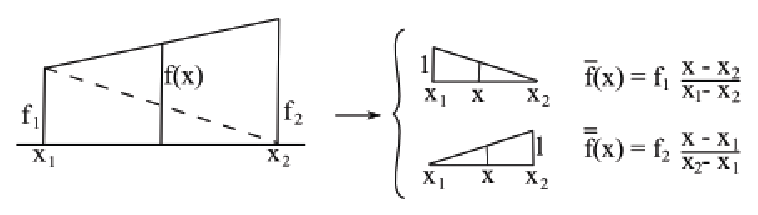
\includegraphics[scale=1.0]{capitulos/capitulo2/figuras/roteiro_da_aula5.eps}
 \caption{?}
 \label{fig:roteiro_da_aula5}
\end{figure}

\textbf{Grau 2}

\begin{figure}[htb]
 \centering
 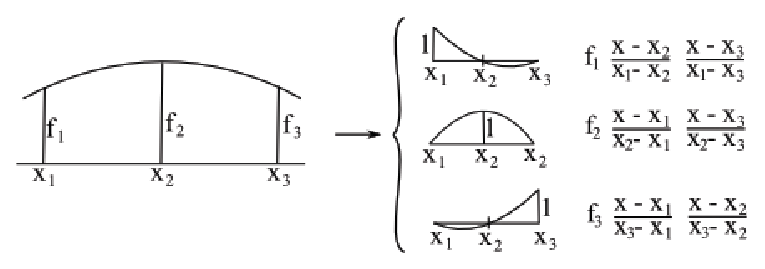
\includegraphics[scale=1.0]{capitulos/capitulo2/figuras/roteiro_da_aula6.eps}
 \caption{?}
 \label{fig:roteiro_da_aula6}
\end{figure}

Grau $n-1 \Rightarrow n$ pontos.

\end{enumerate}


%%% Secao 8
\section{Integração de Funções com Limites Infinitos ou Singularidades (Integrais Impróprias)}

\begin{enumerate}

\item
O integrando tem um limite finito nos limites de interpolação, mas não pode ser calculado nestes limites de integração. Por exemplo, \esp{\displaystyle \frac{\sin x}{x}} em \esp{x=0}:

\[
 \lim_{x \to 0} \, \frac{\sin x}{x} = 1 \, ; \qquad \displaystyle \frac{\sin (0)}{0} \mbox{ (singular)}
\]

\item
O limite superior é $+\infty$ ou o limite inferior é $-\infty$.

\item
Tem uma singularidade integrável em qualquer um dos limites. Por exemplo, \esp{x^{1/2}} em \esp{x=0}

\[
 \begin{array}{ll}
  \displaystyle \int_0^1 \, x^{-1/2} \, dx & = \displaystyle \lim_{h \to 0} \, \int_h^1 \, x^{-1/2} \, dx = \lim_{h \to 0} \, \left. \displaystyle \frac{x^{1/2}}{1/2} \right|_h^1 = \lim_{h \to 0} \, (2\,\sqrt{1} - 2\,\sqrt{h}) \\
  & = 2\,\sqrt{1} = 2
 \end{array}
\]

\item
Tem uma singularidade integrável em um ponto conhecido ou desconhecido entre os limites da integração.

\begin{description}

\item
\textbf{Integral Tipo 1}:

\begin{equation}
 \label{cap2:sec8:eq1}
 I = \int_{-\infty}^\infty exp\,(-x^2)\,dx \qquad \mbox{(caso b)}
\end{equation}

\item
\textbf{Integral Tipo 2}: 

\begin{equation}
 \label{cap2:sec8:eq2}
 I = \int_0^1 \frac{1}{\sqrt{x}\,(e^x + 1)} \, dx
\end{equation}

\begin{itemize}
\item 
O integrando é singular em $x = 0$ ($f(x) \rightarrow \infty$ para $x \rightarrow 0$)
\end{itemize}

\item
\textbf{Integral Tipo 3}:

\begin{equation}
 \label{cap2:sec8:eq3}
 I = \int_0^1 x^{0.7} \, \cos\,(x) \, dx
\end{equation}

\begin{itemize}
\item 
A função (integrando) não é analítica em $x = 0$.
\end{itemize}

\end{description}

\end{enumerate}

\subsection{Tipo 1}

\[
 I = \int_{-\infty}^\infty \, f\,(x) \, dx
 \quad \mbox{ou} \quad
 I = \int_{-\infty}^b \, f\,(x) \, dx
 \quad \mbox{ou} \quad
 I = \int_a^\infty \, f\,(x) \, dx
\]

\textbf{OBS1:} Uma função que é integrável em um domínio infinito ou semi-infinito é aproximadamente zero exceto em uma ?curta? parte do domínio. Por exemplo,

\[
 I = \int_{-\infty}^\infty \, e^{-x^2} \, dx
\]

\begin{figure}[htb]
 \centering
 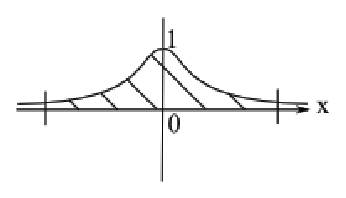
\includegraphics[scale=1.0]{capitulos/capitulo2/figuras/int_func_lim_inf1.eps}
 \caption{?}
 \label{fig:int_func_lim_inf1}
\end{figure}

\textbf{OBS2:} Se $f(x)$ for analítica em $[-\infty,\infty]$, o método mais eficiente para a integração numérica é a regra do trapézio estendida.

\[
 I = h \, \sum_{i=-M}^M \, f\,(x_i)
\]

\begin{figure}[htp]
 \centering
 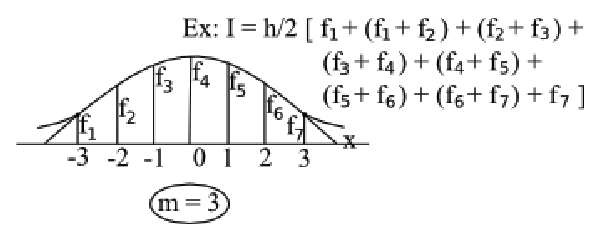
\includegraphics[scale=1.0]{capitulos/capitulo2/figuras/int_func_lim_inf2.eps}
 \caption{?}
 \label{fig:int_func_lim_inf2}
\end{figure}

onde $x_{i} = i \ast h$ e $M$ é um inteiro tal que $\infty$ seja aproximado por $M \ast h$.

\begin{example}
 \esp{I = \displaystyle \frac{1}{\sqrt{\pi}} \, \int_{-\infty}^\infty \, e^{-x^2}} com 20, 40 e 80 intervalos

\textbf{Solução:} \esp{I \approx \displaystyle \frac{1}{\sqrt{\pi}} \, \int_{-10}^{10} \, e^{-x^2}}

\[N = 20 \rightarrow I = 1.000104\]
\[N = 40 \rightarrow I = 1.000001\]
\[N = 80 \rightarrow I = 1.000000\]

Valor exato: $I = 1.000000$
\end{example}

\subsection{Tipo 2}

\[
 I = \int_a^b \, f\,(x) \, dx
\]

onde $a$ e $b$ são finitos, mas $f(x)$ é singular em $a$, $b$ ou ambos.

\begin{enumerate}

\item 
Transformar $[a,b]$ em $[+\infty,-\infty]$ através de mudança de coordenadas.

\item
Aplicar regra do trapézio estendida

\end{enumerate}

\textbf{Mudança de coordenadas}

\[
 \begin{array}{l}
 \xi \qquad \xi\,(?)
 \left\{
 \begin{array}{l}
  \xi\,(a) = - \infty \\
  \xi\,(b) = + \infty
 \end{array}
 \right. \\
 x = x\,(\xi)
 \end{array}
\]

\begin{equation}
 \label{cap2:sec8:eq1}
 I = \int_a^b \, f\,(x) \, dx = \int_{-\infty}^\infty \, f\,(x\,(\xi)) \, \left( \frac{dx}{d\xi} \right) \, dx
\end{equation}

\underline{\textbf{Transformação Exponencial:}}

\begin{equation}
 \label{cap2:sec8:eq2}
 x\,(\xi) = \frac{1}{2} \left[ a + b + (b - a) \, tanh\,(\xi) \right]
\end{equation}

onde

\begin{equation}
 \label{cap2:sec8:eq3}
 tanh\,(\xi) = \frac{e^\xi - e^{-\xi}}{e^\xi + e^{-\xi}}
\end{equation}

\begin{figure}[htb]
 \centering
 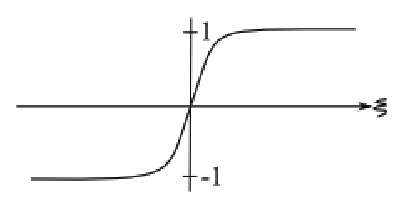
\includegraphics[scale=1.0]{capitulos/capitulo2/figuras/int_func_lim_inf3.eps}
 \caption{?}
 \label{fig:int_func_lim_inf3}
\end{figure}

Para

\[
 \begin{array}{l}
  \xi = + \infty \Rightarrow tanh\,(+\infty) = 1 \Rightarrow x\,(+\infty) = b \\
  \xi = - \infty \Rightarrow tanh\,(-\infty) = -1 \Rightarrow x\,(-\infty) = a
 \end{array}
\]

\begin{equation}
 \label{cap2:sec8:eq4}
 \xi\,(x) = tanh^{-1} \left( \frac{2\,x - a - b}{b - a} \right)\,, \qquad x \in [a,\,b]
\end{equation}

\textbf{OBS1:} Para $\xi = 2.64665 \Rightarrow tanh = 0.99 \Rightarrow x \approx b$

\[
 ?
\]

\textbf{OBS2:} A precisão da integração é função da escolha da transformação.\\

\underline{\textbf{Dupla Exponenciação}}

\begin{equation}
 \label{cap2:sec8:eq5}
 \xi\,(x) = \frac{1}{2} \, \left[ a + b + (b - a) \, tanh \, \left( \frac{\pi}{2} \, sinh\,(\xi) \right) \right]
\end{equation}

\begin{equation}
 \label{cap2:sec8:eq6}
 sinh\,(\xi) = \frac{e^\xi - e^{-\xi}}{2}
\end{equation}

\begin{equation}
 \label{cap2:sec8:eq7}
 cosh\,(\xi) = \frac{e^\xi + e^{-\xi}}{2}
\end{equation}

\begin{equation}
 \label{cap2:sec8:eq8}
 \frac{dx}{d\xi} = \frac{(b-a) \, \displaystyle \frac{\pi}{4} \, cosh(\xi)}{cosh^2 \, \left[ \displaystyle \frac{\pi}{2} \, sinh\,(\xi) \right]}
\end{equation}

Eq. \ref{cap2:sec8:eq5} e \ref{cap2:sec8:eq8} $\rightarrow$ \ref{cap2:sec8:eq1}

\begin{equation}
 \label{cap2:sec8:eq9}
 I = h \, \sum_{k=-N}^N \, f\,(x_k) \, \left( \frac{dx}{d\xi} \right)_k
\end{equation}

onde

\[\xi_{k} = k \ast h\]

(h é predefinido)\\

\textbf{OBS:} Quão grande deve ser $N$?\\

Quando \esp{\xi_{k}} cresce \esp{\Rightarrow cosh^2 \, \left[ \displaystyle \frac{\pi}{2}\,sinh\,(\xi_k) \right] \rightarrow \displaystyle \frac{1}{4} \, exp\,\left[ \frac{\pi}{2} \, exp\,(\xi) \right]}, ou seja, o denominador de $ \displaystyle \frac{dx}{d\xi}$ cresce duplo-exponencialmente podendo causar \textit{overflow}.

Por exemplo,

\[
 \begin{array}{ll}
  & \displaystyle \frac{1}{4} \, exp\,\left[ \frac{\pi}{2} \, exp\,(\xi_k) \right] \approx \underbrace{2 \, \cdot \, 10^{38}}_{\footnotesize{\mbox{máximo número}}} \\
  \Rightarrow & \xi_k \approx 4 \Rightarrow N\,h < 4 \\
  & \\
  & \xi \approx 6.1 \Rightarrow f\,(\xi) \approx 3.6 \, \cdot \, 10^{303}
 \end{array}
\]

Outro exemplo é:

\[
  I = \int_0^2 \sqrt{1 + \frac{1}{x}} \, dx \qquad
 \begin{array}{l}
  a = 0 \\
  b = 2
 \end{array}
\]

Em \esp{x = 0}, \esp{\sqrt{1 + \displaystyle \frac{1}{x}}} é singular.\\

\underline{\textbf{Transformações de Coordenadas}}

\begin{equation}
 \label{cap2:sec8:eq10}
 \begin{array}{ll}
  x_k & = \displaystyle \frac{1}{2} \left[ 0 + 2 + (2 - 0) \, tanh \, \left( \frac{\pi}{2} \, sinh\,(\xi) \right) \right] \vspace*{0.2cm} \\
  x_k & = \displaystyle \frac{1}{2} \left[ 2 + 2 \, tanh \, \left( \frac{\pi}{2} \, sinh\,(\xi_k) \right) \right] \vspace*{0.2cm} \\
      & = 1 + tanh \, \left( \displaystyle \frac{\pi}{2} sinh\,(\xi_k) \right)
 \end{array}
\end{equation}

Substituindo em (a) e adotando os limites de $\xi$ [-4, 4]

{
%\begin{table}[htp]
\footnotesize
	\begin{center}
		\begin{tabular}{|c|c|c|}
		\hline		
		\textbf{N} & \textbf{I} \\
		\hline \hline
		10 & 3.600710 \\
		\hline
		20 & 3.595706 \\
		\hline
		30 & 3.595706 \\
		\hline
		\end{tabular}
	\end{center}
	\label{cap2:sec6:tab3}
%\end{table}
}

%%% Secao 9
\section{Integração Numérica em um Domínio Bidimensional}

\begin{figure}[htb]
 \centering
 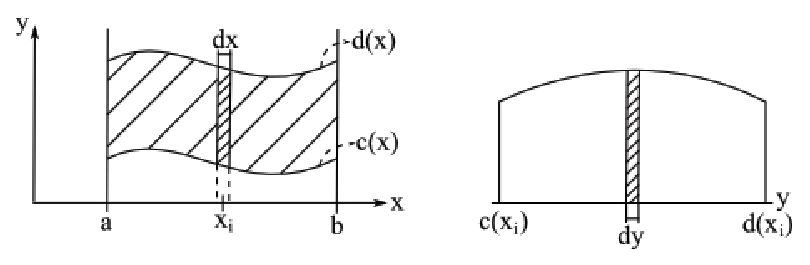
\includegraphics[scale=1.0]{capitulos/capitulo2/figuras/int_num_dom_bid1.eps}
 \caption{Integração Numérica em um Domínio Bidimensional}
 \label{fig:int_num_dom_bid1}
\end{figure}

\begin{equation}
 \label{cap2:sec9:eq1}
 I = \int_a^b \left[ \int_{c\,(x)}^{d\,(x)} \, f\,(x,\,y) \, dy \right] \, dx
\end{equation}

\begin{equation}
 \label{cap2:sec9:eq2}
 G\,(x) = \int_{c\,(x)}^{d\,(x)} \, f\,(x,\,y) \, dy
\end{equation}

\begin{equation}
 \label{cap2:sec9:eq3}
 I = \int_a^b \, G\,(x) \, dx
\end{equation}

\begin{equation}
 \label{cap2:sec9:eq4}
 I = \sum_{i = 0}^N \, w_i \, G\,(x_i)
\end{equation}

\begin{equation}
 \label{cap2:sec9:eq5}
 G\,(x_i) = \sum_{j = 0}^M \, w_j \, f\,(x_i,\,y_j)
\end{equation}

\begin{example}
 Calcule a integral dupla

\[
 I = \int_a^b \left[ \int_{c\,(x)}^{d\,(x)} \, sin\,(x+y) \, dy \right] \, dx
\]

pela regra $\displaystyle \frac{1}{3}$ de Simpson.

\[
 \begin{array}{l}
  a = 1 \\
  b = 3 \\
  c\,(x) = ln\,(x) \\
  d\,(x) = 3 + e^{x/5}
 \end{array}
\]

\textbf{Solução:}

\begin{figure}[htb]
 \centering
 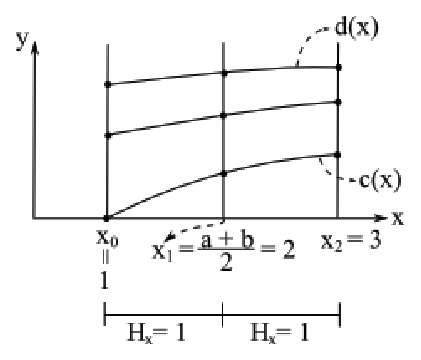
\includegraphics[scale=1.0]{capitulos/capitulo2/figuras/int_num_dom_bid2.eps}
 \caption{?}
 \label{fig:int_num_dom_bid2}
\end{figure}

\[
 \begin{array}{ll}
  I & = \displaystyle \frac{H_x}{3} \, \left[ G\,(x_0) + 4\,G\,(x_1) + G\,(x_2) \right] \vspace*{0.2cm} \\
    & \approx \displaystyle \frac{H_x}{3} \left[ \int_{ln\,(1)}^{3+e^{(1/5)}} sin\,(1+y)\,dy \, + \, 4\,\int_{ln\,(2)}^{3+e^{(2/5)}} sin\,(2+y)\,dy \, + \, \int_{ln\,(3)}^{3+e^{(3/5)}} sin\,(3+y)\,dy \right] \\
    & \approx \displaystyle \frac{1}{3} \left[ \int_0^{4.2214} sin\,(1+y)\,dy \, + \, 4\,\int_{0.6931}^{4.4918} sin\,(2+y)\,dy \, + \, \int_{1.0986}^{4.8221} sin\,(3+y)\,dy \right]
 \end{array}
\]

\[
 \begin{array}{ll}
  G\,(x_0) & \approx \displaystyle \frac{2.11070}{3} \, \left[ sin\,(1+0) + 4\,sin\,(1+2.11070) + sin\,(1+4.2214) \right] \\
           & = 0.064581 \\
  G\,(x_1) & \approx \displaystyle \frac{1.89935}{3} \, \left[ sin\,(2+0.6931) + 4\,sin\,(2+2.59245) + sin\,(2+4.4918) \right] \\
           & = -2.1086 \\
  G\,(x_2) & \approx \displaystyle \frac{1.86175}{3} \, \left[ sin\,(3+1.0986) + 4\,sin\,(3+2.96035) + sin\,(3+4.8221) \right] \\
           & = -0.67454
 \end{array}
\]

\[
 I \approx \frac{1}{3} \, \left[ 0.064581 + (4)\,(-2.1086) - 0.67454 \right] = -3.0148
\]

\end{example}

%%% Secao 10
\section{Integração}

\textbf{Problemas}

\begin{enumerate}
 \item Dada uma função $f(x)$, achar uma função $F(x)$ tal que

\[
 \underbrace{F'(x) = f(x)}_{\footnotesize{\quadricular{\mbox{PROBLEMA DE INTEGRAÇÃO}}}}
\]

\begin{center}
 \small 
\end{center}

\item Dada uma função $f(x) \geq 0$, dar uma definição da área sob a curva $y = f(x)$ que não apele para a intuição geométrica.

\end{enumerate}

\begin{enumerar}  

\item \textbf{Integral Indefinida}

Seja $f(x)$ uma função definida num curto intervalo. Se $F(x)$ é uma função definida no mesmo intervalo e tal que $F'(x) = f(x)$, então dizemos que $F$ é uma integral indefinida de $f$.

\item \textbf{Funções Contínuas}

$f(x)$ é contínua se \esp{\displaystyle \lim_{h \to 0} \, f\,(x+h) = f\,(x) \quad \forall x} para o qual a função está definida.

Toda função derivável é contínua se:

\[
 \frac{f\,(x+h) - f\,(x)}{h}
\]

tem um limite, então:

\[
\begin{array}{ll}
   & \displaystyle \lim_{h \to 0} \, (f\,(x+h) - f\,(x)) \vspace*{0.2cm} \\
 = & \displaystyle \lim_{h \to 0} \, h \, \frac{f\,(x+h) - f\,(x)}{h} \vspace*{0.2cm} \\
 = & \displaystyle \lim_{h \to 0} \, h \, \lim_{h \to 0} \, \frac{f\,(x+h) - f\,(x)}{h} = 0 \\ \\
   & \quadricular{\displaystyle \lim_{h \to 0} \, f\,(x+h) = f\,(x)}
\end{array}
\]

\end{enumerar}



%%% Capitulo 3
\chapter{Diferenciação Numérica}

%%% Secao 1
\section{Expansão de Taylor}

\begin{figure}[htb]
 \centering
 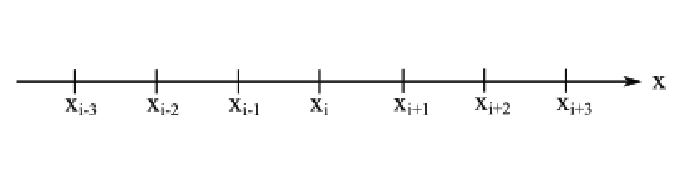
\includegraphics[scale=1.0]{capitulos/capitulo3/figuras/exp_taylor1.eps}
 \caption{?}
 \label{fig:exp_taylor1}
\end{figure}

\begin{equation}
 \label{cap3:sec1:eq1}
 f\,(x_{i+1}) = f\,(x_i+h) = f\,(x_i) + f'(x_i)\,h + \displaystyle \frac{1}{2}\,f''(x_i)\,h^2 + \frac{1}{6}\,f'''(x_i)\,h^3 + \frac{1}{24}\,f^{\,(iv)}\,h^4 \, \ldots
\end{equation}

\begin{equation}
 \label{cap3:sec1:eq2}
 f\,(x_{i-1}) = f\,(x_i-h) = f\,(x_i) - f'(x_i)\,h + \displaystyle \frac{1}{2}\,f''(x_i)\,h^2 - \frac{1}{6}\,f'''(x_i)\,h^3 + \frac{1}{24}\,f^{\,(iv)}\,h^4 + \ldots
\end{equation}

\begin{equation}
 \label{cap3:sec1:eq3}
 f\,(x_{i+2}) = f\,(x_i+2\,h) = f\,(x_i) + f'(x_i)\,2\,h + \displaystyle \frac{1}{2}\,f''(x_i)\,4\,h^2 + \frac{1}{6}\,f'''(x_i)\,8\,h^3 + \frac{1}{24}\,f^{\,(iv)}\,16\,h^4 + \ldots
\end{equation}

\begin{equation}
 \label{cap3:sec1:eq4}
 f\,(x_{i-2}) = f\,(x_i-2\,h) = f\,(x_i) - f'(x_i)\,2\,h + \displaystyle \frac{1}{2}\,f''(x_i)\,4\,h^2 - \frac{1}{6}\,f'''(x_i)\,8\,h^3 + \frac{1}{24}\,f^{\,(iv)}\,16\,h^4 + \ldots
\end{equation}

\begin{equation}
 \label{cap3:sec1:eq5}
 f\,(x_{i+3}) = f\,(x_i+3\,h) = f\,(x_i) + f'(x_i)\,3\,h + \displaystyle \frac{1}{2}\,f''(x_i)\,9\,h^2 + \frac{1}{6}\,f'''(x_i)\,27\,h^3 + \frac{1}{24}\,f^{\,(iv)}\,81\,h^4 + \ldots
\end{equation}

\begin{equation}
 \label{cap3:sec1:eq6}
 f\,(x_{i-3}) = f\,(x_i-3\,h) = f\,(x_i) - f'(x_i)\,3\,h + \displaystyle \frac{1}{2}\,f''(x_i)\,9\,h^2 + \frac{1}{4}\,f'''(x_i)\,27\,h^3 + \frac{1}{24}\,f^{\,(iv)}\,81\,h^4 + \ldots
\end{equation}

\begin{enumerar}
 \item Derivada Primeira (mínimo 2 pontos)

\begin{enumerar}
 \item \textit{Forward Difference}

2 pontos ($x_{i}$ e $x_{i+1}$)

De \ref{cap3:sec1:eq1}:

\[
 \begin{array}{l}
  f'(x_i) = \displaystyle \frac{f\,(x_{i+1}) - f\,(x_i)}{h} - \frac{1}{2} \, f''(x_i) \, h - \frac{1}{6}\,f'''(x_i)\,h^2 - \ldots \vspace*{0.2cm} \\
  f'(x_i) = \displaystyle \frac{f\,(x_{i+1}) - f\,(x_i)}{h} + O\,(h)
 \end{array}
\]

onde

\[
 O\,(h) = -\frac{1}{2}\,f''(x_i)\,h
\]

3 pontos ($x_{i}$, $x_{i+1}$ e $x_{i+2}$)

De -(\ref{cap3:sec1:eq3}) + 4*(\ref{cap3:sec1:eq1}):

\[
 4\,f\,(x_{i+1}) - f\,(x_{i+2}) = 3\,f\,(x_i) + 2\,h\,f'(x_i) - \frac{2}{3}\,h^3\,f'''(x_i)
\]

\[
 f'(x_i) = \frac{-f\,(x_{i+2}) + 4\,f\,(x_{i+1}) - 3\,f\,(x_i)}{2\,h} + O\,(h^2)
\]

onde

\[
 O\,(h^2) = \frac{1}{3} \, h^2 \, f'''(x_i)
\]

4 pontos ($x_{i}$, $x_{i+1}$, $x_{i+2}$ e $x_{i+3}$)

De (\ref{cap3:sec1:eq1}) - $\displaystyle \frac{1}{2}$*(\ref{cap3:sec1:eq3}) + $\displaystyle \frac{1}{9}$*(\ref{cap3:sec1:eq5}):

\[
 \begin{array}{c}
 \underline{
 \begin{array}{rcrrrrrr}
    f_{i+1} & = & f_i & + h\,f'_i & + \displaystyle \frac{h^2}{2} \, f''_i & + \displaystyle \frac{h^3}{6} \, f'''_i & + \displaystyle \frac{h^4}{24} \, f''''_i & + \ldots \vspace*{0.2cm} \\
  - \displaystyle \frac{f_{i+2}}{2} & = & - \displaystyle \frac{f_i}{2} & - h\,f'_i & - \displaystyle \frac{2\,h^2}{2}\,f''_i & - \displaystyle \frac{4\,h^3}{6} \, f'''_i & - \displaystyle \frac{8\,h^4}{24}\,f'''' & - \ldots \vspace*{0.2cm} \\
  + \displaystyle \frac{f_{i+3}}{9} & = & \displaystyle \frac{f_i}{9} & + \displaystyle \frac{h}{3}\,f'_i & + \displaystyle \frac{h^2}{2}\,f''_i & + \displaystyle \frac{3\,h^3}{6}\,f'''_i & + \displaystyle \frac{9\,h^4}{24}\,f'''' & + \ldots
 \end{array}
 } \\
 \displaystyle \frac{f_{i+3}}{9} - \displaystyle \frac{f_{i+2}}{2} + f_{i+1} = \displaystyle \frac{f_i}{9} - \displaystyle \frac{f_i}{2} + f_i + \displaystyle \frac{h}{3}\,f'_i + \displaystyle \frac{h^4}{12}\,f'''' + \ldots
 \end{array}
\]

\[
 f'_i = \frac{2\,f_{i+3} - 9\,f_{i+2} + 18\,f_{i+1} - 11\,f_i}{6\,h} + O\,(h^3)
\]

onde

\[
 O\,(h^3) = - \frac{1}{4} \, h^3 \, f''''_i
\]

\item \textit{Backward Difference}

2 pontos ($x_{i}$ e $x_{i-1}$)

De (\ref{cap3:sec1:eq2}):

\[
 f'(x_i) = \frac{f\,(x_i) - f\,(x_{i-1})}{h} + O\,(h)
\]

onde

\[
 O\,(h) = \frac{1}{2}\,f''(x_i)\,h
\]

3 pontos ($x_{i}$, $x_{i-1}$ e $x_{i-2}$)

\[
 f'(x_i) = \frac{3\,f\,(x_i) - 4\,f\,(x_{i-1}) + f\,(x_{i-2})}{2\,h} + O\,(h^2)
\]

onde

\[
 O\,(h^2) = \frac{1}{3}\,h^2\,f'''(x_i)
\]

4 pontos ($x_{i}$, $x_{i-1}$, $x_{i-2}$ e $x_{i-3}$)

\[
 f'(x_i) = \frac{11\,f_i - 18\,f_{i-1} + 9\,f_{i-2} - 2\,f_{i-3}}{6\,h} + O\,(h^3)
\]

onde

\[
 O\,(h^3) = \frac{1}{4}\,h^3\,f''''_i
\]

\item \textit{Central Difference}

2 pontos ($x_{i+1}$ e $x_{i-1}$)

De (\ref{cap3:sec1:eq1}) - (\ref{cap3:sec1:eq2}):

\[
 f'(x_i) = \frac{f\,(x_{i+1}) - f\,(x_{i-1})}{2\,h} + O\,(h^2)
\]

onde

\[
 O\,(h^2) = -\frac{1}{6}\,h^2\,f'''(x_i)
\]

4 pontos ($x_{i+2}$, $x_{i+1}$, $x_{i-1}$ e $x_{i-2}$) (elimine $f''$ $f'''$)

\[
 f'_i = \frac{-f_{i+2} + 8\,f_{i+1} - 8\,f_{i-1} + f_{i-2}}{12\,h} + O\,(h^2)
\]

onde

\[
 O\,(h^2) = \frac{1}{30} \, h^4 \, f^{\,(iv)}(x_i)
\]

 \end{enumerar}

\item Derivada Segunda (mínimo 3 pontos)

\begin{enumerar}

\item \textit{Forward Difference}

3 pontos ($x_{i}$, $x_{i+1}$ e $x_{i+2}$) elimina $f'(x_{i})$

\[
 f''_i = \frac{f_{i+2} - 2\,f_{i+1} + f_i}{h^2} + O\,(h)
\]

onde

\[
 O\,(h) = -h\,f'''_i
\]

\item \textit{Backward Difference}

\[
 f''_i = \frac{f_i - 2\,f_{i+1} + f_{i-2}}{h^2} + O\,(h)
\]

onde

\[
 O\,(h) = h\,f'''_i
\]

\item \textit{Central Difference}

\[
 f''_i = \frac{f_{i+1} - 2\,f_i + f_{i-1}}{h^2} + O\,(h^2)
\]

onde

\[
 O\,(h^2) = -\frac{1}{2}\,h^2\,f''''_i
\]

\end{enumerar}

\end{enumerar}

\textbf{OBS:}

\begin{itemize}
 \item Uma aproximação para $f^{(p)}$ precisa de pelo menos $p+1$ pontos.

\item As derivadas de ordem menor do que $p$ devem ser eliminadas.

\item O erro é o termo de ordem mais baixa que for truncado.

\end{itemize}



%%% Secao 2
\section{Diferenças Finitas}

\begin{enumerar}

\item Operadores de primeira ordem

\begin{enumerar}

\item \textit{Forward Difference}: \esp{\Delta f_i = f_{i+1} - f_i}

\item \textit{Backward Difference}: \esp{\nabla f_i = f_i - f_{i-1}}

\item Centrada:

\[
 \begin{array}{l}
  \delta f_i = f_{i+\frac{1}{2}} - f_{i-\frac{1}{2}} \\
  \delta f_{i+\frac{1}{2}} = f_{i+1} - f_i
 \end{array}
\]

onde

\[
 f_{i+\frac{1}{2}} = f\,\left(x_i + \frac{h}{2}\right)
\]

\end{enumerar}

\item Operadores de segunda ordem

\begin{enumerar}

\item 
\[
 \begin{array}{c}
  \begin{array}{ll}
   \Delta^2 f_i & = \Delta\,(\Delta\,f_i) = \Delta\,(f_{i+1} - f_i) = \Delta\,f_{i+1} - \Delta f_i \\
                & = f_{i+2} - f_{i+1} - (f_{i+1} - f_i) = f_{i+2} - 2\,f_{i+1} + f_i 
  \end{array} \\ \\
  \quadricular{\Delta^2 f_i = f_{i+2} - 2\,f_{i+1} + f_i}
 \end{array}
\]

\item
\[
 \begin{array}{c}
  \begin{array}{ll}
   \nabla^2 f_i & = \nabla\,(\nabla\,f_i) = \nabla\,(f_i - f_{i-1}) = \nabla\,f_i - \nabla f_{i-1} \\
                & = f_i - f_{i-1} - (f_{i-1} - f_{i-2}) = f_i - 2\,f_{i-1} + f_{i-2} 
  \end{array} \\ \\
  \quadricular{\nabla^2 f_i = f_i - 2\,f_{i-1} + f_{i-2}}
 \end{array}
\]

\item
\[
 \begin{array}{c}
  \begin{array}{ll}
   \delta^2 f_i & = \delta\,(\delta\,f_i) = \delta\,(f_{i+\frac{1}{2}} - f_{i-\frac{1}{2}}) = \delta\,f_{i+\frac{1}{2}} - \delta f_{i-\frac{1}{2}} \\
                & = f_{i+1} - f_i - (f_i - f_{i-1}) = f_{i+1} - 2\,f_i + f_{i-1} 
  \end{array} \\ \\
  \quadricular{\delta^2 f_i = f_{i+1} - 2\,f_i + f_{i-1}}
 \end{array}
\]

\item
\[
 \begin{array}{c}
  \begin{array}{ll}
   \Delta \nabla f_i & = \Delta\,(\nabla\,f_i) = \Delta\,(f_i - f_{i-1}) = \Delta\,f_i - \Delta f_{i-1} \\
                & = f_{i+1} - f_i - f_i + f_{i-1} = f_{i+1} - 2\,f_i + f_{i-1} 
  \end{array} \\ \\
  \quadricular{\Delta \nabla f_i = \delta^2\,f_i = f_{i+1} - 2\,f_i + f_{i-1}}
 \end{array}
\]

\item
\[
 \begin{array}{c}
  \begin{array}{ll}
   \nabla \Delta f_i & = \nabla\,(\Delta\,f_i) = \nabla\,(f_{i+1} - f_i) = \nabla\,f_{i+1} - \nabla f_i \\
                & = f_{i+1} - f_i - f_i + f_{i+1} = f_{i+1} - 2\,f_i + f_{i-1} 
  \end{array} \\ \\
  \quadricular{\nabla \Delta f_i = \delta^2\,f_i = f_{i+1} - 2\,f_i + f_{i-1}}
 \end{array}
\]

\end{enumerar}

\end{enumerar}

\textbf{OBS:}

\begin{enumerate}

\item \esp{\delta^2 = \Delta \nabla = \nabla \Delta}

\item Operadores de ordem mais elevada pode ser obtidos aplicando  os operadores de primeira ordem repetidamente.

\item Se $n$ for par e $\displaystyle m = \frac{n}{2}$, então:

\[
 \nabla^m \Delta^m = \delta^n
\]

\item Operadores diferenciais podem ser aproximados por operadores de diferenças finitas.

\[
 \begin{array}{l}
  \displaystyle \frac{d}{dx} \approx \frac{\Delta}{\Delta x} \vspace*{0.2cm} \\
  \displaystyle \frac{d}{dx} \approx \frac{\nabla}{\nabla x} \vspace*{0.2cm} \\
  \displaystyle \frac{d}{dx} \approx \frac{\delta}{\delta x}
 \end{array} \quad
 \left| \quad
 \begin{array}{l}
  \displaystyle \frac{d^2}{dx^2} \approx \frac{\Delta^2}{\Delta x^2} \vspace*{0.2cm} \\
  \displaystyle \frac{d^2}{dx^2} \approx \frac{\nabla^2}{\nabla x^2} \vspace*{0.2cm} \\
  \displaystyle \frac{d^2}{dx^2} \approx \frac{\nabla}{\nabla x} \, \left( \frac{\Delta}{\Delta x} \right) = \frac{\Delta}{\Delta x} \, \left( \frac{\nabla}{\nabla x} \right) \vspace*{0.2cm} \\
  \displaystyle \frac{d^2}{dx^2} \approx \frac{\delta^2}{\delta x^2}
 \end{array}
 \right.
\]

\end{enumerate}


%%% Secao 3
\section{Método da Diferenciação dos Polinômios de Interpolação de Newton}

\begin{enumerar}

\item O polinômio de interpolação \textit{forward} de \textit{Newton} é:

\begin{equation}
 \label{cap3:sec3:eq1}
 g\,(x) = g\,(x_k + s\,h) = \sum_{n=0}^N \, \left(s \atop n\right) \, \Delta^n \, f_k
\end{equation}

\begin{figure}[htb]
 \centering
 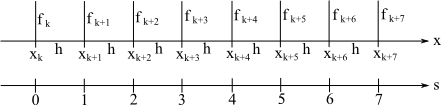
\includegraphics[scale=1.0]{capitulos/capitulo3/figuras/met_dif_pol_int_new1.png}
 \caption{?}
 \label{fig:met_dif_pol_int_new1}
\end{figure}

\begin{equation}
 \label{cap3:sec3:eq2}
 s = \frac{x - x_k}{h}
\end{equation}

\begin{equation}
 \label{cap3:sec3:eq3}
 \left(s \atop n\right) = \frac{s!}{n!\,(s-n)!}
\end{equation}

\begin{equation}
 \label{cap3:sec3:eq4}
 \begin{array}{ll}
  g\,(x) & = g\,(x_k + s\,h) \vspace*{0.2cm} \\
         & = f_k + s\,\Delta\,f_k + \displaystyle \frac{1}{2} \, s\,(s-1)\,\Delta^2\,f_k + \frac{1}{6} \, s\,(s-1)\,(s-2)\,\Delta^3\,f_k \vspace*{0.2cm} \\
         & + \displaystyle \frac{1}{24}\,s\,(s-1)\,(s-2)\,(s-3)\,\Delta^4\,f_k + \ldots + \left(s \atop n\right) \, \Delta^N \, f_k
 \end{array}
\end{equation}

\textbf{OBS:}

O polinômio \esp{g\,(x) = g\,(x_k + s\,h) = \sum_{n=0}^N \, \left( s \atop n \right) \, \Delta^n \, f_k} tem ordem $n$ e passa por $n+1$ pontos amostrais.

\item Para $n = 2 \Rightarrow$ 3 pontos

\begin{equation}
 \label{cap3:sec3:eq5}
 g\,(x) = f_k + s\,\Delta\,f_k + \frac{1}{2}\,s\,(s-1)\,\Delta^2\,f_k
\end{equation}

\begin{equation}
 \label{cap3:sec3:eq6}
 g'\,(x) = \frac{1}{h} \, \left[ \Delta\,f_k + \frac{1}{2}\,(2\,s-1)\,\Delta^2\,f_k \right]
\end{equation}

Para $s = 0$, $1$ e $2$:

\begin{equation}
 \label{cap3:sec3:eq7}
 g'\,(x_k) = \frac{1}{2\,h} \, \left[ 2\,\Delta\,f_k - \Delta^2\,f_k \right] = \frac{1}{2\,h} \, \left[ -f_{k+2} + 4\,f_{k+1} - 3\,f_k \right]
\end{equation}

\begin{equation}
 \label{cap3:sec3:eq8}
 g'\,(x_{k+1}) = \frac{1}{2\,h} \, \left[ 2\,\Delta\,f_k + \Delta^2\,f_k \right] = \frac{1}{2\,h} \, \left[ f_{k+2} - f_k \right]
\end{equation}

\begin{equation}
 \label{cap3:sec3:eq9}
 g'\,(x_{k+2}) = \frac{1}{2\,h} \, \left[ 2\,\Delta\,f_k + 3\,\Delta^2\,f_k \right] = \frac{1}{2\,h} \, \left[ 3\,f_{k+2} - 4\,f_{k+1} + f_k \right]
\end{equation}

$k = i$ (\textit{Forward} 3 pontos)

\begin{equation}
 \label{cap3:sec3:eq10}
 g'\,(x_i) = \frac{1}{2\,h} \, \left[ 2\,\Delta\,f_i - \Delta^2\,f_i \right] = \frac{1}{2\,h} \, \left[ -f_{i+2} + 4\,f_{i+1} - 3\,f_i \right]
\end{equation}

$k + 1 = i$ (Centrada 3 pontos)

\begin{equation}
 \label{cap3:sec3:eq11}
 g'\,(x_i) = \frac{1}{2\,h} \, \left[ 2\,\Delta\,f_{i-1} + \Delta^2\,f_{i-1} \right] = \frac{1}{2\,h} \, \left[ f_{i+1} - f_{i-1} \right]
\end{equation}

$k + 2 = i$ (\textit{Backward} 3 pontos)

\begin{equation}
 \label{cap3:sec3:eq12}
 g'\,(x_i) = \frac{1}{2\,h} \, \left[ 2\,\Delta\,f_{i-2} + 3\,\Delta^2\,f_{i-2} \right] = \frac{1}{2\,h} \, \left[ 3\,f_i - 4\,f_{i-1} + f_{i-2} \right]
\end{equation}

\item Erro

Se tivermos mais um ponto amostral, o polinômio interpolante representa melhor a função interpolada. Assim, o erro do polinômio de \textit{Newton} é representado pelo termo que seria adicionado caso um ponto amostral a mais seja introduzido.

Se, por exemplo, aumentarmos de $n = 2$ para $n = 3$, o termo:

\begin{equation}
 \label{cap3:sec3:eq13}
 \frac{1}{6} \, s\,(s-1)\,(s-2) \, \Delta^3 f_k
\end{equation}

seria acrescido \`a  equa\'c\~ao (\ref{cap3:sec3:eq5}), e sua derivada seria

\begin{equation}
 \label{cap3:sec3:eq14}
 \frac{1}{6\,h} \, \left[ 3\,s^2 - 6\,s + 2 \right] \, \Delta^3 \, f_k
\end{equation}

Para

\begin{equation}
 \label{cap3:sec3:eq15}
 s = 0 \rightarrow \frac{1}{3\,h} \, \Delta^{3}f_{k} \qquad Forward
\end{equation}

\begin{equation}
 \label{cap3:sec3:eq16}
 s = 1 \rightarrow \frac{1}{6\,h} \, \Delta^{3}f_{k} \qquad Centrada
\end{equation}

\begin{equation}
 \label{cap3:sec3:eq17}
 s = 2 \rightarrow \frac{1}{3\,h} \, \Delta^{3}f_{k} \qquad Backward
\end{equation}

\end{enumerar}

\textbf{OBS:}

A e-enésima derivada de $g(x)$ de ordem $n$ é:

\begin{equation}
 \label{cap3:sec3:eq18}
 \frac{d^n}{dx^n} \, g\,(x) = \frac{1}{h^n} \, \Delta^n \, f_i
\end{equation}

Assim,

\begin{equation}
 \label{cap3:sec3:eq19}
 \Delta^n\,f_i \approx h^n \, f^{(n)}(x)
\end{equation}

Portanto, as expressões (\ref{cap3:sec3:eq15}) a (\ref{cap3:sec3:eq17}) ficam:
\[
 \displaystyle \frac{1}{3}\,h^{2}\,f'''_{k}\,, \mbox{ para } s = 0
\]

\[
 \displaystyle -\frac{1}{6}\,h^{2}\,f'''_{k}\,, \mbox{ para } s = 1
\]

\[
 \displaystyle \frac{1}{3}\,h^{2}\,f'''_{k}\,, \mbox{ para } s = 2
\]


%%% Secao 4
\section{Aproximação de Derivadas Parciais por Diferenças Finitas}

A derivada parcial

\[
 f_{,x} = \frac{\partial f\,(x,\,y)}{\partial x} \quad \mbox{em} \quad (x,y) = (x_{0},y_{0})
\]

pode ser deduzida fixando-se \esp{y = y_{0}} e considerando-se \esp{f(x,y_{0})} como uma função de uma variável. Assim, as aproximações de \esp{f_{,x}} por diferenças finitas são:

\[
 f_{,x} \approx \frac{f\,(x_0 + \Delta x,\,y_0) - f\,(x_0,\,y_0)}{\Delta x} \qquad Forward
\]

\[
 f_{,x} \approx \frac{f\,(x_0 + \Delta x,\,y_0) - f\,(x_0 - \Delta x,\,y_0)}{2\,\Delta x} \qquad Central
\]

\[
 f_{,x} \approx \frac{f\,(x_0,\,y_0) - f\,(x_0 - \Delta x,\,y_0)}{\Delta x} \qquad Backward
\]

Diferenças centradas das derivadas parciais $f_{,xx}$, $f_{,yy}$ e $f_{,xy}$:

\[
 f_{,xx} = \frac{\partial^2}{\partial x^2} \, f \approx \frac{f\,(x_0 + \Delta x,\, y_0) - 2\,f\,(x_0,\,y_0) + f\,(x_0 - \Delta x,\,y_0)}{\Delta x^2}
\]

\[
 f_{,yy} = \frac{\partial^2}{\partial y^2} \, f \approx \frac{f\,(x_0,\, y_0 + \Delta y) - 2\,f\,(x_0,\,y_0) + f\,(x_0,\, y_0 - \Delta y)}{\Delta y^2}
\]

\[
 \begin{array}{ll}
  f_{,xy} = \displaystyle \frac{\partial^2}{\partial x \, \partial y} \, f & \approx \displaystyle \frac{f\,(x_0 + \Delta x,\, y_0 + \Delta y) - f\,(x_0 + \Delta x,\,y_0 - \Delta y)}{4\,\Delta x \, \Delta y} \vspace*{0.2cm} \\
   & + \displaystyle \frac{-f\,(x_0 - \Delta x,\, y_0 + \Delta y) + f\,(x_0 - \Delta x,\, y_0 - \Delta y)}{?}
 \end{array}
\]

\subsection{Solução do Problema de Dirichlet}

\textbf{Deformação de uma membrana}\\

EDP: \esp{\displaystyle \frac{\partial^2 u}{\partial x^2} + \frac{\partial^2 u}{\partial y^2} = 0} em \esp{x \in (0,\,1)} e \esp{y \in (0,\,1)} \\

C.C.:

\[
\begin{array}{l}
 u = 0 \quad \mbox{em} \quad
 \left\{
 \begin{array}{l}
  y = 1 \\
  x = 0 \\
  x = 1
 \end{array} \right. \\
 \\
 u\,(x,\,0) = sin\,(\pi \, x) \quad \mbox{com} \quad x \in [0,\,1]
\end{array}
\]

\begin{figure}[htb]
 \centering
 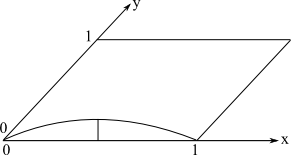
\includegraphics[scale=1.0]{capitulos/capitulo3/figuras/aprox_der_par_dif_fin1.png}
 \caption{?}
 \label{fig:aprox_der_par_dif_fin1}
\end{figure}

\textbf{Solução:}

\begin{enumerate}
 \item Discretizar o domínio numa grade de pontos:

\begin{figure}[htb]
 \centering
 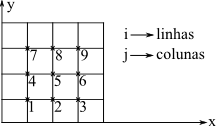
\includegraphics[scale=1.0]{capitulos/capitulo3/figuras/aprox_der_par_dif_fin2.png}
 \caption{?}
 \label{fig:aprox_der_par_dif_fin2}
\end{figure}

\item Escreva a E.D.P. utilizando operadores diferenciais centrados no ponto \esp{(i,\,j)}:

\begin{equation}
 \label{cap3:sec4:eq1}
 \frac{\partial^2 u}{\partial x^2} = \frac{1}{h_x^2} \, (u_{i,j+1} - 2\,u_{i,j} + u_{i,j-1})
\end{equation}

\begin{equation}
 \label{cap3:sec4:eq2}
 \frac{\partial^2 u}{\partial y^2} = \frac{1}{h_y^2} \, (u_{i+1,j} - 2\,u_{i,j} + u_{i-1,j})
\end{equation}

Se \esp{h_x = h_y = h}

\begin{equation}
 \label{cap3:sec4:eq3}
 \frac{\partial^2 u}{\partial x^2} + \frac{\partial^2 u}{\partial y^2} \approx \frac{1}{h^2} \, (u_{i+1,j} + u_{i-1,j} + u_{i,j+1} + u_{i,j-1} - 4\,u_{i,j}) = 0
\end{equation}

\item Definir a célula diferencial

\[
 \begin{array}{lll}
                   & \quadricular{+1} & \vspace*{0.2cm} \\
  \quadricular{+1} & \quadricular{-4} & \quadricular{+1} \vspace*{0.2cm} \\
                   & \quadricular{+1} &
 \end{array}
\]

\item Aplicar a célula a cada ponto interior (P1 a P9):

\[
\begin{array}{l}
 P1: \\
 P2: \\
 P3: \\
 P4: \\
 P5: \\
 P6: \\
 P7: \\
 P8: \\
 P9:
\end{array}
\,
\left[
\begin{array}{rrrrrrrrr}
 -4 &  1 &  0 &  1 &  0 &  0 &  0 &  0 &  0\\
  1 & -4 &  1 &  0 &  1 &  0 &  0 &  0 &  0\\
  0 &  1 & -4 &  0 &  0 &  1 &  0 &  0 &  0\\
  1 &  0 &  0 & -4 &  1 &  0 &  1 &  0 &  0\\
  0 &  1 &  0 &  1 & -4 &  1 &  0 &  1 &  0\\
  0 &  0 &  1 &  0 &  1 & -4 &  0 &  0 &  1\\
  0 &  0 &  0 &  1 &  0 &  0 & -4 &  1 &  0\\
  0 &  0 &  0 &  0 &  1 &  0 &  1 & -4 &  1\\
  0 &  0 &  0 &  0 &  0 &  1 &  0 &  1 & -4
\end{array}
\right]
\,
\left\{
\begin{array}{l}
 u_1 \\
 u_2 \\
 u_3 \\
 u_4 \\
 u_5 \\
 u_6 \\
 u_7 \\
 u_8 \\
 u_9
\end{array}
\right\}
+
\left\{
\begin{array}{c}
 sin\,\left(\frac{\pi}{4}\right) \\
 sin\,\left(\frac{\pi}{2}\right) \\
 sin\,\left(\frac{3\,\pi}{4}\right) \\
 0 \\
 0 \\
 0 \\
 0 \\
 0 \\
 0
\end{array}
\right\}
=
\{0\}
\]

\end{enumerate}


%%% Secao 5
%\section{Método da Secante}
%\index{Método da Secante}

\subsection{Características}

\begin{itemize}
\item Necessita de duas aproximações iniciais da raiz desejada
\item Usa a reta secante passando por dois valores de $f$ consecutivos no processo iterativo.
\end{itemize}

\subsection{Descrição}

\begin{figure}[htb]
  %\index{figura da posição falsa modificado}%
  \setlength{\abovecaptionskip}{20pt}
  %%% o valor default de \abovecaptionskip definido para a classe
  %%% article e de 10pt.
  \centering
  %%% VIDE ABAIXO COMENTARIO SOBRE USO DE DIRETORIOS NO PATHNAME
  %%% DOS ARQUIVOS INCLUIDOS.
  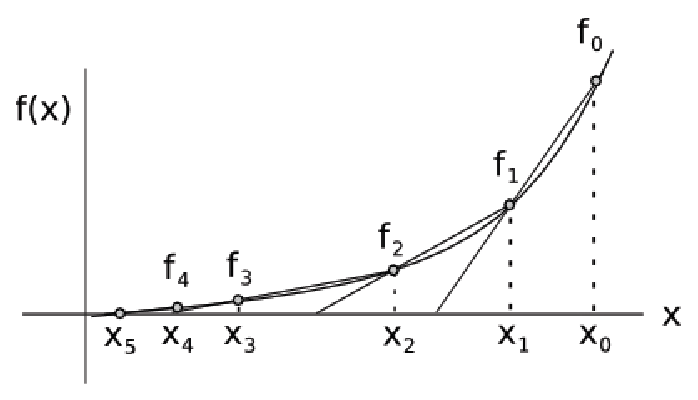
\includegraphics[scale=0.8]{capitulos/capitulo1/figuras/secante1.eps}
  \caption{Descrição do método da secante.}
  \label{fig:secante1}
\end{figure}

Considerando-se $h = x_{n-1} - x_{n-2}$ e utilizando-se \textit{backward} diferença finita para calcular $f'(x_{n-1})$ temos:

\[
 f'(x_{n-1}) = \frac{f(x_{n-1}) - f(x_{n-2})}{x_{n-1} - x_{n-2}}
\]

\[
 x_{n} = x_{n-1} - \frac{f(x_{n-1})}{f'(x_{n-1})} \approx x_{n-1} - \frac{f(x_{n-1})}{\frac{\displaystyle f(x_{n-1}) - f(x_{n-2})}{\displaystyle x_{n-1} - x_{n-2}}}
\]

\[
x_{n} = x_{n-1} - \frac{x_{n-1} - x_{n-2}}{f_{n-1} - f_{n-2}} \ast f_{n-1}
\]

\[
 n = 2, 3, ...
\]

%%% Secao 6
%\section{Condições de Contorno}

Em

\begin{equation}
 \label{cap6:sec5:eq2}
 x = 0 \Rightarrow u\,(0) = 0
 \left\{
 \begin{array}{l}
  \mbox{c c essencial} \\
  \mbox{c c cinemática} \\
  \mbox{c c Dirichlet}
 \end{array}
 \right.
\end{equation}

Em

\begin{equation}
 \label{cap6:sec5:eq3}
 x = L \Rightarrow F\,(L) = c \, L \, \frac{du}{dx} \, (L) = 0
 \left\{
 \begin{array}{l}
  \mbox{c c natural} \\
  \mbox{c c dinâmica} \\
  \mbox{c c de Neuman}
 \end{array}
 \right.
\end{equation}

Problemas de Sturm-Liouville

\begin{equation}
 \label{cap6:sec5:eq4}
 \mbox{ \framebox{ $ - \displaystyle \frac{d}{dx} \, \left(c \, \displaystyle \frac{du}{dx} \right) + q \, u = f $ } }
\end{equation}

\begin{example}

Suponha a equação:

\begin{equation}
 \left\{
 \begin{array}{l}
  - 2 \, y''(x) + y \, (x) = e^{-0.2 \, x} \\
  \mbox{B.c.} \\
  \begin{array}{lll}
   \qquad y\,(0) & = & 1 \\
   \qquad y'(10) & = & -y \, (10)
  \end{array}
 \end{array}
 \right.
\end{equation}

Resolva por diferenças finitas

\begin{figure}[htb]
 \centering
 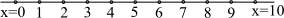
\includegraphics[scale=1.0]{capitulos/capitulo6/figuras/cond_contorno1.png}
 \caption{?}
 \label{fig:cond_contorno1}
\end{figure}

Em

\[
 x = x_i \Rightarrow - 2 \, \left[ \frac{y_{i-1} - 2 \, y_i + y_{i+1}}{h^2} \right] + y_i = e^{-0.2 \, x_i}
\]

\[
 \begin{array}{lll}
  h = 1 & \Rightarrow & -2 \, y_{i-1} + 4 \, y_i - 2 \, y_{i+1} + y_i = e^{-0.2 \, x_i} \\
        & \Rightarrow & \underbrace{\mbox{\framebox{$-2$}}}_{i-1}-\underbrace{\mbox{\framebox{$+5$}}}_{i}-\underbrace{\mbox{\framebox{$-2$}}}_{i+1}
 \end{array}
\]

Aplique nos pontos \esp{1, \, 2, \, \ldots , \, 9}

\[
 \begin{array}{clllllll}
  \mbox{Em } x = 1 & \Rightarrow & -2\,y_0 & +5\,y_1 & -2\,y_2 & & & = e^{-0.2} \nonumber \\
  \mbox{Em } x = 2 & \Rightarrow &         & -2\,y_1 & +5\,y_2 & -2\,y_3 & & = e^{-0.4} \nonumber \\
  \vdots & & & & \vdots & \nonumber \\
  \mbox{Em } x = 9 & \Rightarrow &         &         & -2\,y_8 & +5\,y_9 & -2\,y_{10} & = e^{-1.8} \nonumber \\
 \end{array}
\]

\end{example}


%%% Secao 7
%\section{Problemas Mal Condicionados}

São problemas resolvíveis cujas soluções podem ser bastante imprecisas devido a erros de arredondamento.

Por exemplo,

\[
 \left\{
 \begin{array}{rrrrl}
  0.12065\,x & + & 0.98775\,y & = & 2.01045 \qquad \mbox{(A)} \\
  0.12032\,x & + & 0.98755\,y & = & 2.00555 \qquad \mbox{(B)} \\
 \end{array}
 \right.
\]

\textbf{OBS:} (A) e (B) são bem parecidas

\[
\begin{array}{l}
 x_1 = 14.7403 \\
 y_1 = 0.23942
\end{array}
\]

Simulando um erro nos coeficientes da equação (A)

\[
 2.01045 \rightarrow 2.01045 + 0.001 = 2.01145
\]

\[
 \left\{
 \begin{array}{rrrrl}
  0.12065\,x & + & 0.98775\,y & = & 2.01045 \qquad \mbox{(A')} \\
  0.12032\,x & + & 0.98755\,y & = & 2.00555 \qquad \mbox{(B)} \\
 \end{array}
 \right.
\]

\[
\begin{array}{l}
 x_2 = 17.9756 \\
 y_2 = -0.15928
\end{array}
\]

\textbf{OBS:}

\begin{itemize}

\item Pequenas mudanças em outros coeficientes causam mesmo tipo de comportamento.

\item Erros de arredondamento nos coeficientes podem ocorrer durante o próprio processo de solução.

\end{itemize}

\begin{figure}[htb]
 \centering
 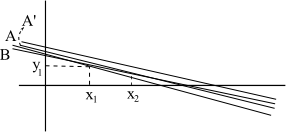
\includegraphics[scale=0.8]{capitulos/capitulo4/figuras/prob_mal_cond1.png}
 \caption{?}
 \label{fig:prob_mal_cond1}
\end{figure}

\textbf{Notas:}

\begin{enumerate}

\item A matriz dos coeficientes de um problema mal condicionado apresenta os seguintes sintomas:

\begin{enumerate}

\item $ a_{ij} + \delta^{ \, \mbox{\tiny{PEQUENO}}} \rightarrow x_k + \Delta^{ \, \mbox{\tiny{GRANDE}}} $

\item $ a_{ii} < a_{kj} $, $ k \neq j $ \, (geralmente)

\item $ det [A] \, det[A]^{-1} \neq 1 $ \, $ (1 \pm \Delta) $

\item $ [A^{-1}]^{-1} \neq A $

\item $ A \, A^{-1} \neq I $

\item $ A^{-1} \, (A^{-1})^{-1} $ \, mais diferente de $I$ do que $ A \, A^{-1} $

\end{enumerate}

\item Pivotação melhora a precisão se o problema for ``moderadamente'' mal condicionado.

\item O melhor procedimento é tentar aumentar ao máximo a precisão (\textit{double})

\[
 \begin{array}{ll}
   \mbox{\textit{Cray}} & \rightarrow \mbox{Precisão simples 8 \textit{bytes} (64 \textit{bits})}\\
   			& \rightarrow \mbox{Precisão dupla 16 \textit{bytes} (128 \textit{bits})}
 \end{array}
\]

\end{enumerate}

\textbf{OBS:} \textit{Singular Value Decomposition of a Matrix}

{
\Large{
\[
 [A_{m \times n}] = [U_{m \times n}] \, [W_{n \times n}] \, [V_{n \times n}]^T
\]
}
}

$U$ e $V$ são matrizes cujas colunas são ortonormais:

\[
 \displaystyle \sum_{i=1}^m U_{ik} \, U_{ij} = \delta_{kj} \, \,
 \left\{
 \begin{array}{l}
   1 \leq k \leq n\\
   1 \leq j \leq n
 \end{array}
 \right.
\]

\[
 \displaystyle \sum_{i=1}^n V_{ik} \, V_{ij} = \delta_{kj}  \, \,
 \left\{
 \begin{array}{l}
   1 \leq k \leq n\\
   1 ? j ? n
 \end{array}
 \right.
\]

{
 \Large{
 \begin{center}
 $
  [A_{n \times n}]^{-1} = [V] \, ${\footnotesize{$
 \left[
 \begin{array}{ccc}
   \ddots & &\\
   & 1/w &\\
   & & \ddots
 \end{array}
 \right]
 $
 }}
 $
 \, [U]^T
 $
 \end{center}
}
}

$c = $ \textit{condition number} $ = \displaystyle \frac{Max(w_i)}{Min(w_i)}$

\begin{itemize}

\item Se $c$ for infinito $ \Rightarrow A$ é singular.

\item Se $c$ muito grande $ \Rightarrow A$ é mal condicionada.

\begin{itemize}

\item muito grande $ \Rightarrow \displaystyle \frac{1}{c} \approx
\left\{
\begin{array}{ll}
 10^{-6} & \mbox{Precisão simples}\\
 10^{-12} & \mbox{Precisão dupla}
\end{array}
\right.
$

\end{itemize}

\end{itemize}


%%% Secao 8
%\section{Integração de Funções com Limites Infinitos ou Singularidades (Integrais Impróprias)}

\begin{enumerate}

\item
O integrando tem um limite finito nos limites de interpolação, mas não pode ser calculado nestes limites de integração. Por exemplo, \esp{\displaystyle \frac{\sin x}{x}} em \esp{x=0}:

\[
 \lim_{x \to 0} \, \frac{\sin x}{x} = 1 \, ; \qquad \displaystyle \frac{\sin (0)}{0} \mbox{ (singular)}
\]

\item
O limite superior é $+\infty$ ou o limite inferior é $-\infty$.

\item
Tem uma singularidade integrável em qualquer um dos limites. Por exemplo, \esp{x^{1/2}} em \esp{x=0}

\[
 \begin{array}{ll}
  \displaystyle \int_0^1 \, x^{-1/2} \, dx & = \displaystyle \lim_{h \to 0} \, \int_h^1 \, x^{-1/2} \, dx = \lim_{h \to 0} \, \left. \displaystyle \frac{x^{1/2}}{1/2} \right|_h^1 = \lim_{h \to 0} \, (2\,\sqrt{1} - 2\,\sqrt{h}) \\
  & = 2\,\sqrt{1} = 2
 \end{array}
\]

\item
Tem uma singularidade integrável em um ponto conhecido ou desconhecido entre os limites da integração.

\begin{description}

\item
\textbf{Integral Tipo 1}:

\begin{equation}
 \label{cap2:sec8:eq1}
 I = \int_{-\infty}^\infty exp\,(-x^2)\,dx \qquad \mbox{(caso b)}
\end{equation}

\item
\textbf{Integral Tipo 2}: 

\begin{equation}
 \label{cap2:sec8:eq2}
 I = \int_0^1 \frac{1}{\sqrt{x}\,(e^x + 1)} \, dx
\end{equation}

\begin{itemize}
\item 
O integrando é singular em $x = 0$ ($f(x) \rightarrow \infty$ para $x \rightarrow 0$)
\end{itemize}

\item
\textbf{Integral Tipo 3}:

\begin{equation}
 \label{cap2:sec8:eq3}
 I = \int_0^1 x^{0.7} \, \cos\,(x) \, dx
\end{equation}

\begin{itemize}
\item 
A função (integrando) não é analítica em $x = 0$.
\end{itemize}

\end{description}

\end{enumerate}

\subsection{Tipo 1}

\[
 I = \int_{-\infty}^\infty \, f\,(x) \, dx
 \quad \mbox{ou} \quad
 I = \int_{-\infty}^b \, f\,(x) \, dx
 \quad \mbox{ou} \quad
 I = \int_a^\infty \, f\,(x) \, dx
\]

\textbf{OBS1:} Uma função que é integrável em um domínio infinito ou semi-infinito é aproximadamente zero exceto em uma ?curta? parte do domínio. Por exemplo,

\[
 I = \int_{-\infty}^\infty \, e^{-x^2} \, dx
\]

\begin{figure}[htb]
 \centering
 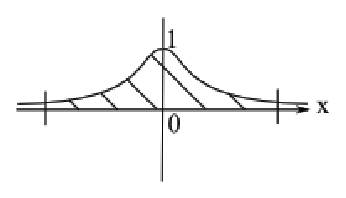
\includegraphics[scale=1.0]{capitulos/capitulo2/figuras/int_func_lim_inf1.eps}
 \caption{?}
 \label{fig:int_func_lim_inf1}
\end{figure}

\textbf{OBS2:} Se $f(x)$ for analítica em $[-\infty,\infty]$, o método mais eficiente para a integração numérica é a regra do trapézio estendida.

\[
 I = h \, \sum_{i=-M}^M \, f\,(x_i)
\]

\begin{figure}[htp]
 \centering
 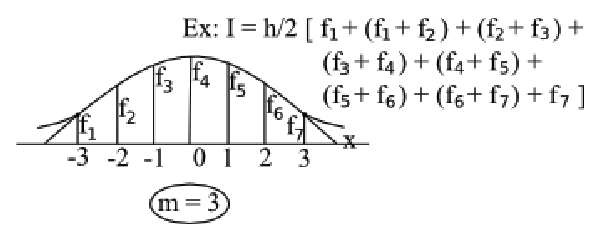
\includegraphics[scale=1.0]{capitulos/capitulo2/figuras/int_func_lim_inf2.eps}
 \caption{?}
 \label{fig:int_func_lim_inf2}
\end{figure}

onde $x_{i} = i \ast h$ e $M$ é um inteiro tal que $\infty$ seja aproximado por $M \ast h$.

\begin{example}
 \esp{I = \displaystyle \frac{1}{\sqrt{\pi}} \, \int_{-\infty}^\infty \, e^{-x^2}} com 20, 40 e 80 intervalos

\textbf{Solução:} \esp{I \approx \displaystyle \frac{1}{\sqrt{\pi}} \, \int_{-10}^{10} \, e^{-x^2}}

\[N = 20 \rightarrow I = 1.000104\]
\[N = 40 \rightarrow I = 1.000001\]
\[N = 80 \rightarrow I = 1.000000\]

Valor exato: $I = 1.000000$
\end{example}

\subsection{Tipo 2}

\[
 I = \int_a^b \, f\,(x) \, dx
\]

onde $a$ e $b$ são finitos, mas $f(x)$ é singular em $a$, $b$ ou ambos.

\begin{enumerate}

\item 
Transformar $[a,b]$ em $[+\infty,-\infty]$ através de mudança de coordenadas.

\item
Aplicar regra do trapézio estendida

\end{enumerate}

\textbf{Mudança de coordenadas}

\[
 \begin{array}{l}
 \xi \qquad \xi\,(?)
 \left\{
 \begin{array}{l}
  \xi\,(a) = - \infty \\
  \xi\,(b) = + \infty
 \end{array}
 \right. \\
 x = x\,(\xi)
 \end{array}
\]

\begin{equation}
 \label{cap2:sec8:eq1}
 I = \int_a^b \, f\,(x) \, dx = \int_{-\infty}^\infty \, f\,(x\,(\xi)) \, \left( \frac{dx}{d\xi} \right) \, dx
\end{equation}

\underline{\textbf{Transformação Exponencial:}}

\begin{equation}
 \label{cap2:sec8:eq2}
 x\,(\xi) = \frac{1}{2} \left[ a + b + (b - a) \, tanh\,(\xi) \right]
\end{equation}

onde

\begin{equation}
 \label{cap2:sec8:eq3}
 tanh\,(\xi) = \frac{e^\xi - e^{-\xi}}{e^\xi + e^{-\xi}}
\end{equation}

\begin{figure}[htb]
 \centering
 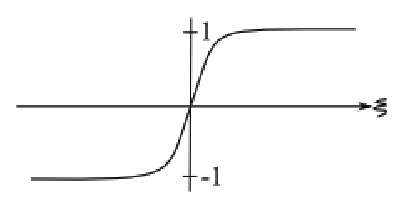
\includegraphics[scale=1.0]{capitulos/capitulo2/figuras/int_func_lim_inf3.eps}
 \caption{?}
 \label{fig:int_func_lim_inf3}
\end{figure}

Para

\[
 \begin{array}{l}
  \xi = + \infty \Rightarrow tanh\,(+\infty) = 1 \Rightarrow x\,(+\infty) = b \\
  \xi = - \infty \Rightarrow tanh\,(-\infty) = -1 \Rightarrow x\,(-\infty) = a
 \end{array}
\]

\begin{equation}
 \label{cap2:sec8:eq4}
 \xi\,(x) = tanh^{-1} \left( \frac{2\,x - a - b}{b - a} \right)\,, \qquad x \in [a,\,b]
\end{equation}

\textbf{OBS1:} Para $\xi = 2.64665 \Rightarrow tanh = 0.99 \Rightarrow x \approx b$

\[
 ?
\]

\textbf{OBS2:} A precisão da integração é função da escolha da transformação.\\

\underline{\textbf{Dupla Exponenciação}}

\begin{equation}
 \label{cap2:sec8:eq5}
 \xi\,(x) = \frac{1}{2} \, \left[ a + b + (b - a) \, tanh \, \left( \frac{\pi}{2} \, sinh\,(\xi) \right) \right]
\end{equation}

\begin{equation}
 \label{cap2:sec8:eq6}
 sinh\,(\xi) = \frac{e^\xi - e^{-\xi}}{2}
\end{equation}

\begin{equation}
 \label{cap2:sec8:eq7}
 cosh\,(\xi) = \frac{e^\xi + e^{-\xi}}{2}
\end{equation}

\begin{equation}
 \label{cap2:sec8:eq8}
 \frac{dx}{d\xi} = \frac{(b-a) \, \displaystyle \frac{\pi}{4} \, cosh(\xi)}{cosh^2 \, \left[ \displaystyle \frac{\pi}{2} \, sinh\,(\xi) \right]}
\end{equation}

Eq. \ref{cap2:sec8:eq5} e \ref{cap2:sec8:eq8} $\rightarrow$ \ref{cap2:sec8:eq1}

\begin{equation}
 \label{cap2:sec8:eq9}
 I = h \, \sum_{k=-N}^N \, f\,(x_k) \, \left( \frac{dx}{d\xi} \right)_k
\end{equation}

onde

\[\xi_{k} = k \ast h\]

(h é predefinido)\\

\textbf{OBS:} Quão grande deve ser $N$?\\

Quando \esp{\xi_{k}} cresce \esp{\Rightarrow cosh^2 \, \left[ \displaystyle \frac{\pi}{2}\,sinh\,(\xi_k) \right] \rightarrow \displaystyle \frac{1}{4} \, exp\,\left[ \frac{\pi}{2} \, exp\,(\xi) \right]}, ou seja, o denominador de $ \displaystyle \frac{dx}{d\xi}$ cresce duplo-exponencialmente podendo causar \textit{overflow}.

Por exemplo,

\[
 \begin{array}{ll}
  & \displaystyle \frac{1}{4} \, exp\,\left[ \frac{\pi}{2} \, exp\,(\xi_k) \right] \approx \underbrace{2 \, \cdot \, 10^{38}}_{\footnotesize{\mbox{máximo número}}} \\
  \Rightarrow & \xi_k \approx 4 \Rightarrow N\,h < 4 \\
  & \\
  & \xi \approx 6.1 \Rightarrow f\,(\xi) \approx 3.6 \, \cdot \, 10^{303}
 \end{array}
\]

Outro exemplo é:

\[
  I = \int_0^2 \sqrt{1 + \frac{1}{x}} \, dx \qquad
 \begin{array}{l}
  a = 0 \\
  b = 2
 \end{array}
\]

Em \esp{x = 0}, \esp{\sqrt{1 + \displaystyle \frac{1}{x}}} é singular.\\

\underline{\textbf{Transformações de Coordenadas}}

\begin{equation}
 \label{cap2:sec8:eq10}
 \begin{array}{ll}
  x_k & = \displaystyle \frac{1}{2} \left[ 0 + 2 + (2 - 0) \, tanh \, \left( \frac{\pi}{2} \, sinh\,(\xi) \right) \right] \vspace*{0.2cm} \\
  x_k & = \displaystyle \frac{1}{2} \left[ 2 + 2 \, tanh \, \left( \frac{\pi}{2} \, sinh\,(\xi_k) \right) \right] \vspace*{0.2cm} \\
      & = 1 + tanh \, \left( \displaystyle \frac{\pi}{2} sinh\,(\xi_k) \right)
 \end{array}
\end{equation}

Substituindo em (a) e adotando os limites de $\xi$ [-4, 4]

{
%\begin{table}[htp]
\footnotesize
	\begin{center}
		\begin{tabular}{|c|c|c|}
		\hline		
		\textbf{N} & \textbf{I} \\
		\hline \hline
		10 & 3.600710 \\
		\hline
		20 & 3.595706 \\
		\hline
		30 & 3.595706 \\
		\hline
		\end{tabular}
	\end{center}
	\label{cap2:sec6:tab3}
%\end{table}
}

%%% Secao 9
%\section{Integração Numérica em um Domínio Bidimensional}

\begin{figure}[htb]
 \centering
 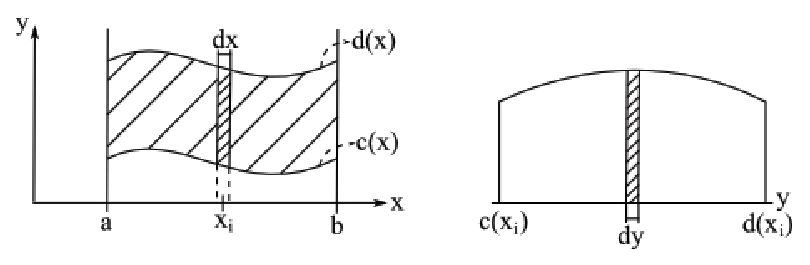
\includegraphics[scale=1.0]{capitulos/capitulo2/figuras/int_num_dom_bid1.eps}
 \caption{Integração Numérica em um Domínio Bidimensional}
 \label{fig:int_num_dom_bid1}
\end{figure}

\begin{equation}
 \label{cap2:sec9:eq1}
 I = \int_a^b \left[ \int_{c\,(x)}^{d\,(x)} \, f\,(x,\,y) \, dy \right] \, dx
\end{equation}

\begin{equation}
 \label{cap2:sec9:eq2}
 G\,(x) = \int_{c\,(x)}^{d\,(x)} \, f\,(x,\,y) \, dy
\end{equation}

\begin{equation}
 \label{cap2:sec9:eq3}
 I = \int_a^b \, G\,(x) \, dx
\end{equation}

\begin{equation}
 \label{cap2:sec9:eq4}
 I = \sum_{i = 0}^N \, w_i \, G\,(x_i)
\end{equation}

\begin{equation}
 \label{cap2:sec9:eq5}
 G\,(x_i) = \sum_{j = 0}^M \, w_j \, f\,(x_i,\,y_j)
\end{equation}

\begin{example}
 Calcule a integral dupla

\[
 I = \int_a^b \left[ \int_{c\,(x)}^{d\,(x)} \, sin\,(x+y) \, dy \right] \, dx
\]

pela regra $\displaystyle \frac{1}{3}$ de Simpson.

\[
 \begin{array}{l}
  a = 1 \\
  b = 3 \\
  c\,(x) = ln\,(x) \\
  d\,(x) = 3 + e^{x/5}
 \end{array}
\]

\textbf{Solução:}

\begin{figure}[htb]
 \centering
 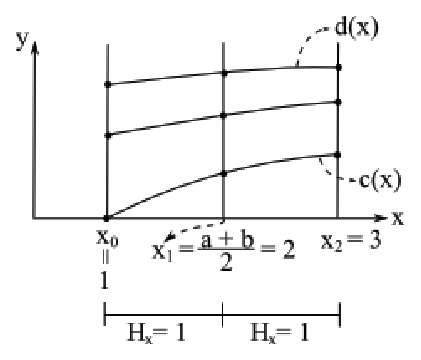
\includegraphics[scale=1.0]{capitulos/capitulo2/figuras/int_num_dom_bid2.eps}
 \caption{?}
 \label{fig:int_num_dom_bid2}
\end{figure}

\[
 \begin{array}{ll}
  I & = \displaystyle \frac{H_x}{3} \, \left[ G\,(x_0) + 4\,G\,(x_1) + G\,(x_2) \right] \vspace*{0.2cm} \\
    & \approx \displaystyle \frac{H_x}{3} \left[ \int_{ln\,(1)}^{3+e^{(1/5)}} sin\,(1+y)\,dy \, + \, 4\,\int_{ln\,(2)}^{3+e^{(2/5)}} sin\,(2+y)\,dy \, + \, \int_{ln\,(3)}^{3+e^{(3/5)}} sin\,(3+y)\,dy \right] \\
    & \approx \displaystyle \frac{1}{3} \left[ \int_0^{4.2214} sin\,(1+y)\,dy \, + \, 4\,\int_{0.6931}^{4.4918} sin\,(2+y)\,dy \, + \, \int_{1.0986}^{4.8221} sin\,(3+y)\,dy \right]
 \end{array}
\]

\[
 \begin{array}{ll}
  G\,(x_0) & \approx \displaystyle \frac{2.11070}{3} \, \left[ sin\,(1+0) + 4\,sin\,(1+2.11070) + sin\,(1+4.2214) \right] \\
           & = 0.064581 \\
  G\,(x_1) & \approx \displaystyle \frac{1.89935}{3} \, \left[ sin\,(2+0.6931) + 4\,sin\,(2+2.59245) + sin\,(2+4.4918) \right] \\
           & = -2.1086 \\
  G\,(x_2) & \approx \displaystyle \frac{1.86175}{3} \, \left[ sin\,(3+1.0986) + 4\,sin\,(3+2.96035) + sin\,(3+4.8221) \right] \\
           & = -0.67454
 \end{array}
\]

\[
 I \approx \frac{1}{3} \, \left[ 0.064581 + (4)\,(-2.1086) - 0.67454 \right] = -3.0148
\]

\end{example}

%%% Secao 10
%\section{Integração}

\textbf{Problemas}

\begin{enumerate}
 \item Dada uma função $f(x)$, achar uma função $F(x)$ tal que

\[
 \underbrace{F'(x) = f(x)}_{\footnotesize{\quadricular{\mbox{PROBLEMA DE INTEGRAÇÃO}}}}
\]

\begin{center}
 \small 
\end{center}

\item Dada uma função $f(x) \geq 0$, dar uma definição da área sob a curva $y = f(x)$ que não apele para a intuição geométrica.

\end{enumerate}

\begin{enumerar}  

\item \textbf{Integral Indefinida}

Seja $f(x)$ uma função definida num curto intervalo. Se $F(x)$ é uma função definida no mesmo intervalo e tal que $F'(x) = f(x)$, então dizemos que $F$ é uma integral indefinida de $f$.

\item \textbf{Funções Contínuas}

$f(x)$ é contínua se \esp{\displaystyle \lim_{h \to 0} \, f\,(x+h) = f\,(x) \quad \forall x} para o qual a função está definida.

Toda função derivável é contínua se:

\[
 \frac{f\,(x+h) - f\,(x)}{h}
\]

tem um limite, então:

\[
\begin{array}{ll}
   & \displaystyle \lim_{h \to 0} \, (f\,(x+h) - f\,(x)) \vspace*{0.2cm} \\
 = & \displaystyle \lim_{h \to 0} \, h \, \frac{f\,(x+h) - f\,(x)}{h} \vspace*{0.2cm} \\
 = & \displaystyle \lim_{h \to 0} \, h \, \lim_{h \to 0} \, \frac{f\,(x+h) - f\,(x)}{h} = 0 \\ \\
   & \quadricular{\displaystyle \lim_{h \to 0} \, f\,(x+h) = f\,(x)}
\end{array}
\]

\end{enumerar}



%%% Capitulo 4
\chapter{Solução de Sistemas de Equações Algébricas Lineares}

%%% Secao 1
\section{Métodos de Eliminação de Gauss e Gauss-Jordan}

\begin{enumerar}

\item Gauss

\[
\begin{array}{rrrrrrr}
 2\,x_1 & + & 1\,x_2 & - & 3\,x_3 & = & -1 \\
-1\,x_1 & + & 3\,x_2 & + & 2\,x_3 & = & 12 \\
 3\,x_1 & + & 1\,x_2 & - & 3\,x_3 & = & 0
\end{array}
\]

Passo 1: Tornar os termos da primeira coluna abaixo da diagonal zero, utilizando combinação linear das linhas correspondentes com a primeira linha:

\[
 a'_{ij} = a_{ij} - a_{ij}/a_{11} \times a_{1j}
 \qquad
 \left\{
  \begin{array}{ll}
   i & = 2\,,\, N \\
   j & = 1\,,\, N
  \end{array}
 \right.
\]

$
 \qquad \quad \, 2\,x_1 \,\,\,\, + \,\,\,\, 1\,x_2 \,\,\,\, - \,\,\,\, 3\,x_3 \,\,\,\, = \,\,\,\,  -1 \\
 -\frac{1}{2}
 \left\{
 \begin{array}{rrrrrrl}
 -1\,x_1 & + & 3\,x_2 & + & 2\,x_3 & = & 12 \\
  3\,x_1 & + & 1\,x_2 & - & 3\,x_3 & = & 0 \\
  0\,x_1 & + & \displaystyle \frac{7}{2}\,x_2 & + & \displaystyle \frac{1}{2}\,x_3 & = & \displaystyle \frac{23}{2} \qquad L'_2 = L_2 - \left(-\displaystyle\frac{1}{2}\right) \, L_1
 \end{array}
 \right.
$

\[
 \begin{array}{rrrrrrl}
  3\,x_1 & + & 1\,x_2 & - & 3\,x_3 & = & 0 \\
  \displaystyle \frac{3}{2}\,2\,x_1 & + & \displaystyle \frac{3}{2}\,1\,x_2 & + & \displaystyle \frac{3}{2}\,(-3)\,x_3 & = & \displaystyle \frac{3}{2}\,(-1) \\
  0\,x_1 & - & \displaystyle \frac{1}{2}\,x_2 & ? & \displaystyle \frac{3}{2}\,x_3 & = & \displaystyle \frac{3}{2} \qquad \qquad L'_3 = L_3 - \left(-\displaystyle\frac{3}{2}\right) \, L_1
 \end{array}
\]

\end{enumerar}

%%% Secao 2
\section{Método de Eliminação de Gauss Padrão com Pivotação}

\textbf{Notas:} O método da eliminação de Gauss não funciona se o primeiro coeficiente da primeira linha for zero ou um coeficiente da diagonal se tornar zero durante o processo.

\begin{itemize}
 \item Pivotação é usada para mudar a ordem seqüencial das linhas para:

\begin{itemize}
 \item Evitar que o coeficiente da diagonal se torne zero.

\item Trazer o maior coeficiente abaixo da diagonal para a diagonal.

\item A mudança da ordem das linhas (equações) não afetam a solução do sistema.

\item Mesmo que o termo da diagonal não seja zero, colocar um coeficiente dominante na diagonal melhora a precisão.
\end{itemize}

\end{itemize}

\begin{example}

\begin{equation}
 \label{cap4:sec2:eq1}
 \left[
 \begin{array}{rrr}
   0 & 10 & 1 \\
   1 & 3 & -1 \\
   2 & 4 & 1
 \end{array}
 \right]
 \,
 \left[
 \begin{array}{r}
   x_1 \\
   x_2 \\
   x_3
 \end{array}
 \right]
 =
 \left[
 \begin{array}{r}
   2 \\
   6 \\
   5
 \end{array}
 \right]
 \quad
 \begin{array}{l}
   \\
   L'_2 = L_2 - \frac{1}{0}\,L_1 \quad \mbox{(impossível)} \vspace*{0.05cm}\\
   L'_3 = L_3 - \frac{2}{0}\,L_1 \quad \mbox{(impossível)}
 \end{array}
\end{equation}

Troca linha 1 com linha 3:

\begin{equation}
 \label{cap4:sec2:eq2}
 \left[
 \begin{array}{rrr}
   2 & 4 & 1 \\
   1 & 3 & -1 \\
   0 & 10 & 1
 \end{array}
 \right]
 \,
 \left[
 \begin{array}{r}
   x_1 \\
   x_2 \\
   x_3
 \end{array}
 \right]
 =
 \left[
 \begin{array}{r}
   5 \\
   6 \\
   2
 \end{array}
 \right]
 \quad
 \begin{array}{l}
   L_1 \\
   L'_2 = L_2 - \frac{1}{2}\,L_1 \vspace*{0.05cm}\\
   L'_3 = L_3 - \frac{0}{2}\,L_1
 \end{array}
\end{equation}

\begin{equation}
 \label{cap4:sec2:eq3}
 \left[
 \begin{array}{rrr}
   2 & 4 & 1 \\
   0 & 1 & -3/2 \\
   0 & 10 & 1
 \end{array}
 \right]
 \,
 \left[
 \begin{array}{r}
   x_1 \\
   x_2 \\
   x_3
 \end{array}
 \right]
 =
 \left[
 \begin{array}{r}
   5 \\
   7/2 \\
   2
 \end{array}
 \right]
\end{equation}

Troca linha 2 com linha 3:

\begin{equation}
 \label{cap4:sec2:eq4}
 \left[
 \begin{array}{rrr}
   2 & 4 & 1 \\
   0 & 10 & 1 \\
   0 & 1 & -3/2
 \end{array}
 \right]
 \,
 \left[
 \begin{array}{r}
   x_1 \\
   x_2 \\
   x_3
 \end{array}
 \right]
 =
 \left[
 \begin{array}{r}
   5 \\
   2 \\
   7/2
 \end{array}
 \right]
 \quad
 \begin{array}{l}
   \\
   \\
   L'_3 = L_3 - \frac{1}{10}\,L_2
 \end{array}
\end{equation}

\begin{equation}
 \label{cap4:sec2:eq5}
 \left[
 \begin{array}{rrr}
   2 & 4 & 1 \\
   0 & 10 & 1 \\
   0 & 0 & -16/5
 \end{array}
 \right]
 \,
 \left[
 \begin{array}{r}
   x_1 \\
   x_2 \\
   x_3
 \end{array}
 \right]
 =
 \left[
 \begin{array}{r}
   5 \\
   2 \\
   33/5
 \end{array}
 \right]
\end{equation}

Retro-substituição:

\[
 x_3 = \frac{33}{5} : \frac{-16}{5} = - \frac{33}{5} \, \frac{5}{16} = -2.0625
\]

\[
 x_2 = \frac{1}{10} \, [2 - 1 \, (-2.0625)] = 0.40625
\]

\[
 x_1 = \frac{1}{2} \, [5 - (4\,0.40625 + 1\,(-2.0625))] = 2.7187
\]

Gauss-Jordan

\[
 \left[
 \begin{array}{rrr}
   2 & 0 & 3/5 \\
   0 & 10 & 1 \\
   0 & 0 & -16/5
 \end{array}
 \right]
 \,
 \left[
 \begin{array}{r}
   x_1 \\
   x_2 \\
   x_3
 \end{array}
 \right]
 =
 \left[
 \begin{array}{r}
   21/5 \\
   2 \\
   33/5
 \end{array}
 \right]
 \quad
 \begin{array}{l}
   L'_1 = L_1 - \frac{2}{5}\,L_2 \\
   \\
   \,
 \end{array}
\]

Divisão de $L_{3} : (-16/5)$

\[
 \left[
 \begin{array}{rrr}
   2 & 0 & 3/5 \\
   0 & 10 & 1 \\
   0 & 0 & 1
 \end{array}
 \right]
 \,
 \left[
 \begin{array}{r}
   x_1 \\
   x_2 \\
   x_3
 \end{array}
 \right]
 =
 \left[
 \begin{array}{r}
   21/5 \\
   2 \\
   -2.0625
 \end{array}
 \right]
 \quad
 \begin{array}{l}
   L'_1 = L_1 - \frac{3/5}{1}\,L_3 \\
   L'_2 = L_2 - \frac{1}{1}\,L_3 \\
   \,
 \end{array}
\]

\[
 \left[
 \begin{array}{rrr}
   2 & 0 & 0 \\
   0 & 10 & 0 \\
   0 & 0 & 1
 \end{array}
 \right]
 \,
 \left[
 \begin{array}{r}
   x_1 \\
   x_2 \\
   x_3
 \end{array}
 \right]
 =
 \left[
 \begin{array}{r}
   5.4375 \\
   4.0625 \\
   -2.0625
 \end{array}
 \right]
\]

\[
 \left[
 \begin{array}{rrr}
   1 & 0 & 0 \\
   0 & 1 & 0 \\
   0 & 0 & 1
 \end{array}
 \right]
 \,
 \left[
 \begin{array}{r}
   x_1 \\
   x_2 \\
   x_3
 \end{array}
 \right]
 =
 \left[
 \begin{array}{r}
   2.71875 \\
   0.40625 \\
   -2.06250
 \end{array}
 \right]
\]

\end{example}

\textbf{Nota:} Se a pivotação não impedir que apareça zero na diagonal, o problema é não resolvível.

\begin{example}

Exemplo real:

\[
\left[
 \begin{array}{llll}
  1.334 \cdot 10^{-4} & 4.123 \cdot 10^1 & 7.912 \cdot 10^2 & -1.544 \cdot 10^3 \\
  1.777 & 2.367 \cdot 10^{-5} & 2.070 \cdot 10^1 & -9.035 \cdot 10^1 \\
  9.188 & 0 & -1.0150 \cdot 10^1 & 1.988 \cdot 10^{-4} \\
  1.002 \cdot 10^2 & 1.442 \cdot 10^4 & -7.014 \cdot 10^2 & 5.321
 \end{array}
\right]
\,
\left[
 \begin{array}{llll}
  -711.5698662 \\
  -67.87297633 \\
  -0.961801200 \\
  13824.12100
 \end{array}
\right]
\]

\textbf{Solução:}

\begin{enumerar}

\item Precisão simples

{
\footnotesize
\centering
	
\begin{tabular}{|c|c|c|}
	\hline
	\textbf{i} & \textbf{$x_i$ \, (s/ pivotação)} & \textbf{$x_i$ \, (c/ pivotação)} \\
	\hline \hline
	$1$ & $0.95506$ & $0.99998$ \\
	\hline
	$2$ & $1.00816$ & $1.$ \\
	\hline
	$3$ & $0.96741$ & $1.$ \\
	\hline
	$4$ & $0.98352$ & $1.$ \\
	\hline
\end{tabular}
}

\item Precisão dupla

{
\footnotesize
\centering
	
\begin{tabular}{|c|c|c|}
	\hline
	\textbf{i} & \textbf{$x_i$ \, (s/ pivotação)} & \textbf{$x_i$ \, (c/ pivotação)} \\
	\hline \hline
	$1$ & $0.9999\,9999\,9801\,473$ & $1.0000\,0000\,0000\,002$ \\
	\hline
	$2$ & $1.0000\,0000\,0000\,784$ & $1.0000\,0000\,0000\,000$ \\
	\hline
	$3$ & $0.9999\,9999\,9984\,678$ & $1.0000\,0000\,0000\,000$ \\
	\hline
	$4$ & $0.9999\,9999\,9921\,696$ & $1.0000\,0000\,0000\,000$ \\
	\hline
\end{tabular}
}

\end{enumerar}

\end{example}




%%% Secao 3
\section{Problemas não resolvíveis}

\begin{description}

\item[] \textbf{OBS:} Nem sempre um sistema de equações é resolvível:

\begin{enumerar}

\item

\begin{figure}[htb]
 \centering
 \begin{minipage}[c]{3cm}
    \[
     \begin{array}{rrrrr}
      -x & + & y & = & 1 \\
      -2\,x & + & 2\,y & = & 2
     \end{array}
    \]
 \end{minipage}\hspace*{2cm}
 \begin{minipage}[c]{5cm}
    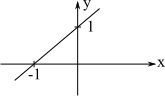
\includegraphics[scale=0.8]{capitulos/capitulo4/figuras/prob_nao_resol1.png}
    \caption{?}
    \label{fig:prob_nao_resol1}
 \end{minipage}
\end{figure}

\item

\begin{figure}[htb]
 \centering
 \begin{minipage}[c]{3cm}
    \[
     \begin{array}{rrrrr}
      -x & + & y & = & 1 \\
      -x & + & y & = & 0
     \end{array}
    \]
 \end{minipage}\hspace*{2cm}
 \begin{minipage}[c]{5cm}
    \includegraphics[scale=0.8]{capitulos/capitulo4/figuras/prob_nao_resol2.png}
    \caption{?}
    \label{fig:prob_nao_resol2}
 \end{minipage}
\end{figure}

\item

\begin{figure}[htb]
 \centering
 \begin{minipage}[c]{3cm}
    \[
     \begin{array}{rrrrr}
      -x & + & y & = & 1 \\
      x & + & 2\,y & = & -2 \\
      2\,x & - & y & = & 0
     \end{array}
    \]
 \end{minipage}\hspace*{2cm}
 \begin{minipage}[c]{5cm}
    \includegraphics[scale=0.8]{capitulos/capitulo4/figuras/prob_nao_resol3.png}
    \caption{?}
    \label{fig:prob_nao_resol3}
 \end{minipage}
\end{figure}

\end{enumerar}

\end{description}

\begin{description}

\item[] No conjunto:

\begin{enumerar}

\item As duas equações são idênticas. Qualquer ponto satisfazendo uma equação satisfaz outra. Assim, o sistema tem infinitas soluções (linearmente independentes).

\item Inconsistente se lado esquerdo de uma das equações for eliminado por combinação linear das outras equações, enquanto o lado direito permanece diferente de zero.

\item Duas incógnitas e três equações nunca são satisfeitas simultaneamente.

\end{enumerar}

\item[] Solução única (condições necessárias):

\begin{itemize}

\item Número de equações igual ao número de incógnitas.

\item Equações são L.I. (linearmente independentes)

\end{itemize}

\end{description}

%%% Secao 4
\section{Matrizes, Vetores e Inversão de Matrizes}

\begin{itemize}

\item Matrizes quadradas e retangulares.

\item Operações: adição, subtração, multiplicação e divisão

\begin{itemize}
 \item Divisão $B^{-1}A = C$ só existe se $B$ for quadrada.
\end{itemize}

\item Vetores

\item Produto de matriz por vetor

\end{itemize}

\subsection{Matriz Nula}

\[ A_{ij} = 0\]

\subsection{Matriz Identidade}

\[
  I =
  \left\{
    \begin{array}{ll}
      1, & \mbox{se $i = j$} \\
      0, & \mbox{se $i \neq j$}
    \end{array}
  \right.  %%% o ``.'' coloca um delimitador invisivel.
\]

\subsection{Matriz Transposta de A}

\[ A^{T} \Rightarrow a^{T}_{ij} = a_{ji} \]

\subsection{Matriz Inversa}

$A^{-1}$ de uma matriz quadrada

\[ AA^{-1} = A^{-1}A = I \]

Se $BA = I$ ou $AB = I$ então $B = A^{-1}$

\subsection{Matriz Ortogonal}

Matrizes cujas colunas são ortogonais entre si:

\[ Q^{T}Q = I;\,\, QQ^{T} = I;\,\, Q^{T} = Q^{-1} \]

\subsection{Vetor Nulo}

\[ a_{i} = 0 \]

\subsection{Vetor Unitário}

\[
  u = \left[
    \begin{array}{c}
      1 \\
      0 \\
      0 
    \end{array}
    \right];\,\,
  v = \left[
    \begin{array}{c}
      0 \\
      1 \\
      0 
    \end{array}
    \right]
  w = \left[
    \begin{array}{c}
      0 \\
      0 \\
      1 
    \end{array}
    \right]
\]

\[
u = \frac{\vec{u}}{|\vec{u}|}
\]

\subsection{Vetor Transposto}

\[
  v = \left[
    \begin{array}{c}
      x_1 \\
      x_2 \\
      x_3 
    \end{array}
    \right]
\,\,\,
  v^T = \left[
    \begin{array}{ccc}
      x_1 & x_2 & x_3 
    \end{array}
    \right]
\]

\subsection{Inversão de uma Matriz}

\[ Ax = y\]

Suponha que o processo de eliminação de Gauss-Jordan seja resumido na operação matricial.

\[ G \, A \, x = G \, y \]

Fazendo $G \, A = I$, temos:

\[ I \, x = G \, y \]

Assim

\begin{center}
$ G = A^{-1} \,$ ou $\, G \, I = A^{-1} $
\end{center}

\[
 \left[
  \begin{array}{ccc}
    a_{11} & a_{12} & a_{13}\\
    a_{21} & a_{22} & a_{23}\\
    a_{31} & a_{32} & a_{33}
  \end{array}
 \right]
  \,\,
\left[
  \begin{array}{ccc}
    1 & 0 & 0\\
    0 & 1 & 0\\
    0 & 0 & 1
  \end{array}
 \right]
\]

Aplicar Gauss-Jordan ou Gauss ``padrão'' (pivotação pode ser utilizada).

\[ [A][X] = [I] \]

\begin{example}

Calcule a inversa de

\[
 A =
  \left[
  \begin{array}{ccc}
    2 & 1 & -3\\
    -1 & 3 & 2\\
    3 & 1 & -3
  \end{array}
  \right]
\]

Resposta:

\[
 A^{-1} =
  \left[
  \begin{array}{ccc}
    -1 & 0 & 1\\
    0.27272 & 0.27272 & -0.09??0\\
    -0.90909 & 0.09090 & 0.63636
  \end{array}
  \right]
\]

\end{example}


%%% Secao 5
\section{Decomposição LU}

\[ A = L \, U \]

$L =$ matriz triangular inferior com diagonal 1

$U =$ matriz triangular superior com diagonal $\neq$ 1

\begin{center}
$ A \, x = y \Rightarrow L \, U \, x = y \,$
 ou
$
  \,
  \begin{array}{l}
    L \, z = y\\
    U \, x = z
  \end{array}
$
\end{center}

\[
 \left[
  \begin{array}{cccccc}
   a_{11} & a_{12} & \cdots & a_{1j} & \cdots & a_{1n} \\
   a_{21} & a_{22} & \cdots & a_{2j} & \cdots & a_{2n} \\
   \vdots & \vdots & \vdots & \vdots & \ddots & \vdots \\
   a_{i1} & a_{i2} & \cdots & a_{ij} & \cdots & a_{in} \\
   \vdots & \vdots & \vdots & \vdots & \ddots & \vdots \\
   a_{n1} & a_{n2} & \cdots & a_{nj} & \cdots & a_{nn}
  \end{array}
 \right]
 =
 \left[
  \begin{array}{cccc}
   1 & 0 & \cdots & 0 \\
   l_{21} & 1 & \cdots & 0 \\
   \vdots & \vdots & \ddots & \vdots \\
   l_{n1} & l_{n2} & \cdots & 1
  \end{array}
 \right]
 \left[
  \begin{array}{cccc}
   u_{11} & u_{12} & \cdots & u_{1n} \\
   0 & u_{22} & \cdots & u_{2n} \\
   \vdots & \vdots & \ddots & \vdots \\
   0 & 0 & \cdots & u_{nn}
  \end{array}
 \right]
\]

\[
a_{ij} = \sum_{k = 1}^{N}l_{ik} \, u_{kj}
=
 \left\{
  \begin{array}{ll}
   \displaystyle \sum_{k = 1}^{i}l_{ik} \, u_{kj}, & \mbox{se $i \leq j$}\\
   \displaystyle \sum_{k = 1}^{j}l_{ik} \, u_{kj}, & \mbox{se $i > j$}
  \end{array}
 \right.
\]

\begin{center}
$
\displaystyle a_{ij} = \sum_{k = 1}^{i-1}l_{ik} \, u_{kj} + l_{ii} \, u_{ij} \Rightarrow
$
\framebox{
$
\displaystyle  u_{ij} = a_{ij} - \sum_{k = 1}^{i-1} l_{ik} \, u_{kj}
$
}
\end{center}

\begin{center}
$
\displaystyle a_{ij} = \sum_{k = 1}^{j-1}l_{ik} \, u_{kj} + l_{ij} \, u_{jj} \Rightarrow
$
\framebox{
$
\displaystyle  l_{ij} = \frac{ a_{ij} - \displaystyle \sum_{k = 1}^{j-1} l_{ik} \, u_{kj} }{u_{jj}}
$
}
\end{center}

\noindent
\textbf{Resumo:}

\begin{enumerar}

\item Qualquer matriz não singular pode ser decomposta na forma $A = L \, U$.

\item Se um sistema de equações lineares tiver de ser resolvido repetidamente para múltiplos lados ?direitos?, a decomposição $L \, U$ é recomendada.

\item A matriz $U$ é idêntica a obtida no processo de eliminação de Gauss.

\item $L \, U$ é útil no cálculo do determinante.

\end{enumerar}


%%% Secao 6
\section{Cálculo de Determinante}

A toda matriz quadrada $A = [a_{ij}]$ de ordem $n$ cujos elementos são números complexos, associa-se um único número denominado determinante de $A$.

\begin{center}
$ det \, A \,$ ou $\, |A| $
\end{center}

Se $E$ for o conjunto de matrizes quadradas de ordem $n$ e $C$ for o conjunto dos números complexos, podemos construir $f: E \rightarrow C$ de modo que

\begin{enumerate}

\item Se $n = 1$, $A = [a_{11}]$ e $det \, A = a_{11}$

\item Se $ n \geq 2$, $det \, A = \displaystyle \sum_{i=1}^{n}(-1)^{i+1} \, a_{i1} \, D_{i1}$

onde $D_{i1}$ é o menor complementar do elemento $a_{i1}$ de $A$ (determinante da matriz obtida eliminando-se a linha $i$ e a coluna 1 de $A$)

\end{enumerate}

Chamando-se $ A_{ij} = (-1)^{i+j} \, D_{ij} $ de cofator do elemento $a_{ij}$, podemos escrever

\[ det \, A = \displaystyle \sum_{i=1}^{n} a_{i1} \, A_{i1} \]

O teorema de Laplace generaliza esta definição para

\begin{center}

$ det \, A = \displaystyle \sum_{i=1}^{n} a_{ij} \, A{ij} $ fixando-se $j, 1 \leq j \leq n$

\end{center}

ou

\begin{center}

$ det \, A = \displaystyle \sum_{j=1}^{n} a_{ij} \, A{ij} $ fixando-se $i, 1 \leq i \leq n$

\end{center}

\subsection{Propriedades dos Determinantes}

\textbf{P1:} $ det \, M^T = det \, M $.\\

\textbf{P2:} Se os elementos de uma linha (coluna) de uma matriz quadrada $ M = [a_{ij}] $, de ordem $n$, forem todos iguais a zero, então $ det \, M = 0 $.\\

\textbf{P3:} Multiplicando-se uma linha (ou coluna) de uma matriz quadrada $ M = [a_{ij}] $ por um número $k$, o determinante da nova matriz $ N = [b_{ij}] $ que se obtém será:

\[
det \, N = k \, det \, M
\]

\textbf{P4:} Se a coluna $q$ de uma matriz quadrada $ M = [a_{ij}] $ de ordem $n$ puder ser escrita como:

\[ a_{iq} = b_{iq} + c_{iq} \]

então $ det \, M = det \, M' + det \, M''$ onde $M'$ é igual a $M$ trocando-se a coluna $q$ por $b_{iq}$ e $M''$ é a matriz obtida procurando-se a coluna $q$ de $M$ por $c_{iq}$.\\

\textbf{P5:} Se $[N]_{n \times m}$ é obtida de $[M]_{n \times m}$ trocando-se duas linhas (ou colunas) então:

\[
 det \,N = -det \, M
\]

\textbf{P6:} Se duas linhas ou colunas de $M$ forem iguais, então:

\[
 det \, N = 0
\]

\textbf{P7:} (Teorema de \textit{Cauchy}) O produto escalar de uma linha (ou coluna) pelo vetor de cofatores de uma outra linha (ou coluna) é zero.\\

\textbf{P8:} Se duas linhas (ou colunas) de $[M]_{n \times n}$ forem proporcionais, então:

\[
 det \, M = 0
\]

\textbf{P9:} Se a matriz quadrada $[M]_{n \times n}$ tem uma linha (ou coluna) que é combinação linear das outras linhas (ou colunas), então:

\[
 det \, M = 0
\]

\textbf{P10:} Se adicionarmos a uma linha (ou coluna) de $[M]_{n \times n}$ uma combinação linear das outras formando uma matriz $[N]_{n \times n}$, então:

\[
 det \, N = det \, M
\]

\textbf{P11:} Se $[M]_{n \times n}$ for triangular, $det \, M$ é o produto dos elementos da diagonal:

\[
 det M \, = a_{11} \, a_{22} \, a_{33} \, \ldots \, a_{nn}
\]

\textbf{P12:} Se $[M]_{n \times n}$ for triangular com relação à diagonal secundária, então:

\begin{center}
 $det \, M = (-1)^{ \displaystyle \frac{n \, (n - 1)}{2}} \times $ (Produto dos termos da diagonal secundária)
\end{center}

\textbf{P13:} Se $[N]_{n \times n} = k \, [M]_{n \times n}$ então:

\[
 det \, [N] = k^n \, (det \, [M])
\]

\textbf{P14:} (Teorema de \textit{Binet}) Se $[C]_{n \times n} = [A]_{n \times n} \, [B]_{n \times n}$, então

\[
 det \, [C] = (det \, [A]) \, (det \, [B])
\]

\subsection{Cálculo Numérico do Determinante de $[A]_{n \times n}$}

\[
 [A] = [A] \, [U]
\]

\begin{center}
 Por \textbf{P14} $\Rightarrow det \, [A] = det [L] \, det \, [U]$
\end{center}

\begin{center}
 Por \textbf{P11} $\Rightarrow det \, [L] = 1$ e $det \, [U] = \displaystyle \prod_{i=1}^n \, u_{ii}$
\end{center}

\textbf{OBS:} Como $[U]$ pode ser obtida por eliminação de Gauss padrão podemos utilizar ``\textit{forward} ? ?''

%%% Secao 7
\section{Problemas Mal Condicionados}

São problemas resolvíveis cujas soluções podem ser bastante imprecisas devido a erros de arredondamento.

Por exemplo,

\[
 \left\{
 \begin{array}{rrrrl}
  0.12065\,x & + & 0.98775\,y & = & 2.01045 \qquad \mbox{(A)} \\
  0.12032\,x & + & 0.98755\,y & = & 2.00555 \qquad \mbox{(B)} \\
 \end{array}
 \right.
\]

\textbf{OBS:} (A) e (B) são bem parecidas

\[
\begin{array}{l}
 x_1 = 14.7403 \\
 y_1 = 0.23942
\end{array}
\]

Simulando um erro nos coeficientes da equação (A)

\[
 2.01045 \rightarrow 2.01045 + 0.001 = 2.01145
\]

\[
 \left\{
 \begin{array}{rrrrl}
  0.12065\,x & + & 0.98775\,y & = & 2.01045 \qquad \mbox{(A')} \\
  0.12032\,x & + & 0.98755\,y & = & 2.00555 \qquad \mbox{(B)} \\
 \end{array}
 \right.
\]

\[
\begin{array}{l}
 x_2 = 17.9756 \\
 y_2 = -0.15928
\end{array}
\]

\textbf{OBS:}

\begin{itemize}

\item Pequenas mudanças em outros coeficientes causam mesmo tipo de comportamento.

\item Erros de arredondamento nos coeficientes podem ocorrer durante o próprio processo de solução.

\end{itemize}

\begin{figure}[htb]
 \centering
 \includegraphics[scale=0.8]{capitulos/capitulo4/figuras/prob_mal_cond1.png}
 \caption{?}
 \label{fig:prob_mal_cond1}
\end{figure}

\textbf{Notas:}

\begin{enumerate}

\item A matriz dos coeficientes de um problema mal condicionado apresenta os seguintes sintomas:

\begin{enumerate}

\item $ a_{ij} + \delta^{ \, \mbox{\tiny{PEQUENO}}} \rightarrow x_k + \Delta^{ \, \mbox{\tiny{GRANDE}}} $

\item $ a_{ii} < a_{kj} $, $ k \neq j $ \, (geralmente)

\item $ det [A] \, det[A]^{-1} \neq 1 $ \, $ (1 \pm \Delta) $

\item $ [A^{-1}]^{-1} \neq A $

\item $ A \, A^{-1} \neq I $

\item $ A^{-1} \, (A^{-1})^{-1} $ \, mais diferente de $I$ do que $ A \, A^{-1} $

\end{enumerate}

\item Pivotação melhora a precisão se o problema for ``moderadamente'' mal condicionado.

\item O melhor procedimento é tentar aumentar ao máximo a precisão (\textit{double})

\[
 \begin{array}{ll}
   \mbox{\textit{Cray}} & \rightarrow \mbox{Precisão simples 8 \textit{bytes} (64 \textit{bits})}\\
   			& \rightarrow \mbox{Precisão dupla 16 \textit{bytes} (128 \textit{bits})}
 \end{array}
\]

\end{enumerate}

\textbf{OBS:} \textit{Singular Value Decomposition of a Matrix}

{
\Large{
\[
 [A_{m \times n}] = [U_{m \times n}] \, [W_{n \times n}] \, [V_{n \times n}]^T
\]
}
}

$U$ e $V$ são matrizes cujas colunas são ortonormais:

\[
 \displaystyle \sum_{i=1}^m U_{ik} \, U_{ij} = \delta_{kj} \, \,
 \left\{
 \begin{array}{l}
   1 \leq k \leq n\\
   1 \leq j \leq n
 \end{array}
 \right.
\]

\[
 \displaystyle \sum_{i=1}^n V_{ik} \, V_{ij} = \delta_{kj}  \, \,
 \left\{
 \begin{array}{l}
   1 \leq k \leq n\\
   1 ? j ? n
 \end{array}
 \right.
\]

{
 \Large{
 \begin{center}
 $
  [A_{n \times n}]^{-1} = [V] \, ${\footnotesize{$
 \left[
 \begin{array}{ccc}
   \ddots & &\\
   & 1/w &\\
   & & \ddots
 \end{array}
 \right]
 $
 }}
 $
 \, [U]^T
 $
 \end{center}
}
}

$c = $ \textit{condition number} $ = \displaystyle \frac{Max(w_i)}{Min(w_i)}$

\begin{itemize}

\item Se $c$ for infinito $ \Rightarrow A$ é singular.

\item Se $c$ muito grande $ \Rightarrow A$ é mal condicionada.

\begin{itemize}

\item muito grande $ \Rightarrow \displaystyle \frac{1}{c} \approx
\left\{
\begin{array}{ll}
 10^{-6} & \mbox{Precisão simples}\\
 10^{-12} & \mbox{Precisão dupla}
\end{array}
\right.
$

\end{itemize}

\end{itemize}


%%% Secao 8
\section{Soluções de Sistemas de Equações com M equações e N incógnitas}

Seja

\[
 A \, x = y
\]

Se $ det \, A = 0 $, a solução do sistema não é única.

Por exemplo,

\[
 \left[
  \begin{array}{cc}
   1 & 1 \\
   0 & 0
  \end{array}
 \right]
 \left[
  \begin{array}{c}
   x \\
   y
  \end{array}
 \right]
 =
 \left[
  \begin{array}{c}
   1 \\
   0
  \end{array}
 \right]
  \begin{array}{r}
   (A) \\
   (B)
  \end{array}
\]

Solução de (B): $ S_B = \{ \, \forall(x,y) \, | \, (x,y) \in \varmathbb{R}^2 \, \} $

Solução de (A): $ S_A = \{ \, (x,y) \in \varmathbb{R}^2 \, \, | \, \, y = 1 - x \, \} $\\

$ S_B \cap S_A = S_A $

$ S_A = $ reta ($ y = 1 -x $)

\begin{figure}[htb]
 \centering
 \includegraphics[scale=1.0]{capitulos/capitulo4/figuras/sol_sist_equa_m_equa_n_incog1.png}
 \caption{?}
 \label{fig:sol_sist_equa_m_equa_n_incog1}
\end{figure}

Por exemplo,

\[
 \left\{
  \begin{array}{rrrrrrrrrrr}
   -1 \, u & + & 2 \, v & + & 2 \, w & + & x & - & 2 \, y & = & 2\\
   3 \, u & - & 6 \, v & - & w & + & 5 \, x & - & 4 \,y & = & 1\\
   2 \, u & - & 4 \, v & - & 1.5 \, w & + & 2 \, x & - & y & = & -0.5
  \end{array}
 \right.
\]

\[
 \begin{array}{|rrrrrr|}
	\hline
	\textbf{u} & \textbf{v} & \textbf{w} & \textbf{x} & \textbf{y} & \textbf{l.d.}\\
	\hline \hline
	-1 & 2 & 2 & 1 & -2 & 2\\
	\hline
	3 & -6 & -1 & 5 & -4 & 1\\
	\hline
	2 & -4 & -1.5 & 2 & -1 & -0.5\\
	\hline
 \end{array}
\]

\begin{description}

\item[i)] Pivotação

\hspace*{2 cm}
$
 \left\{
  \begin{array}{rrrrrr|r}
   3 & -6 & -1 & 5 & -4 & 1 &\\
   -1 & 2 & 2 & 1 & -2 & 2 & L'_2 = L_2 + \frac{1}{3} \, L_1\\
   2 & -4 & -1.5 & 2 & -1 & -0.5 & L'_3 = L_3 - \frac{2}{3} \, L_1
  \end{array}
 \right.
$

\hspace*{2 cm}
$
 \left\{
  \begin{array}{lrlrrr|c}
   3^{\mbox{\tiny{(PIVÔ)}}} & -6 & -1 & 5 & -4 & 1 &\\
   0 & 0 & 5/3^{\mbox{\tiny{(PIVÔ)}}} & 8/3 & - 10/3 & - 7/3 &\\
   0 & 0 & - 5/6 & - 4/3 & 5/3 & - 7/6 & L'_3 = L_3 - \frac{1}{2} \, L_2
  \end{array}
 \right.
$

\hspace*{2 cm}
$
 \left\{
  \begin{array}{rrrrrr}
   3 & -6 & -1 & 5 & -4 & 1\\
   0 & 0 & 5/3 & 8/3 & - 10/3 & - 7/3\\
   0 & 0 & 0 & 0 & 0 & 0
  \end{array}
 \right.
$

\hspace*{2 cm}
$
 \left[
  \begin{array}{cc}
   3 & -1\\
   0 & 5/3
  \end{array}
 \right]
 \left[
  \begin{array}{c}
   u\\
   w
  \end{array}
 \right]
 =
 \left[
  \begin{array}{cccccc}
   u & = & 0.8 & + 2 \, v & -2.2 \, x & + 2 \,y\\
   w & = & 1.4 &          & -1.6 \, x & + 2 \,y
  \end{array}
 \right]
$

\end{description}

Exemplo 2: Gauss-Jordan

\[
 \begin{array}{|rrrrrr|}
	\hline
	\textbf{u} & \textbf{v} & \textbf{w} & \textbf{x} & \textbf{y} & \textbf{l.d.}\\
	\hline \hline
	2 & 3 & 1 & 4 & 1 & 6\\
	\hline
	2 & 3 & 1 & 1 & -1 & 1\\
	\hline
	4 & 6 & -1 & 1 & 2 & 5\\
	\hline
 \end{array}
\]

\begin{description}

\item[i)] Pivotação

\hspace*{2 cm}
$
 \left\{
  \begin{array}{rrrrrr|l}
   4 & 6 & -1 & 1 & 2 & 5 & (: 4)\\
   2 & 3 & 1 & 1 & -1 & 1 & L'_2 = L_2 - 2 \, L_1\\
   2 & 3 & 1 & 4 & 1 & 6 & L'_3 = L_3 - 2 \, L_1
  \end{array}
 \right.
$

\hspace*{2 cm}
$
 \left\{
  \begin{array}{rrrrrr|l}
   1 & 1.5 & -0.25 & 0.25 & 0.5 & 1.25 & L'_1 = L_1 + 0.25 \, L_2\\
   0 & 0 & 1.5 & 0.5 & -2 & -1.5 & (: 1.5)\\
   0 & 0 & 1.5 & 3.5 & 0 & 3.5 & L'_3 = L_3 - 1.5 \, L_2
  \end{array}
 \right.
$

\hspace*{2 cm}
$
 \left\{
  \begin{array}{rrrrrr|l}
   1 & 1.5 & 0 & 0.3333 & 0.1667 & 1 &\\
   0 & 0 & 1 & 0.3333 & -1.3333 & -1 &\\
   0 & 0 & 0 & 3 & 2 & 5 & (: 3)
  \end{array}
 \right.
$

\hspace*{2 cm}
$
 \left\{
  \begin{array}{rrrrrr|l}
   1 & 1.5 & 0 & 1/3 & 1/6 & 1 & L'_1 = L_1 - \frac{1}{3} \, L_3\\
   0 & 0 & 1 & 1/3 & -4/3 & -1 & L'_2 = L_2 - \frac{1}{3} \, L_3\\
   0 & 0 & 0 & 1 & 2/3 & 5/3 &
  \end{array}
 \right.
$

\end{description}

\textbf{OBS:} As variáveis básicas são aquelas cujos coeficientes são unitários e os únicos não nulos na coluna.

\hspace*{2 cm}
$
% \left\{
  \begin{array}{rrrr}
   u = & \displaystyle \frac{4}{9}    & - \, \displaystyle \frac{3}{2} \, v & + \displaystyle \frac{1}{18} \, y\\\\
   w = & - \, \displaystyle \frac{14}{9} &                 & + \displaystyle \frac{14}{9} \, y\\\\
   x = & \displaystyle \frac{5}{3}    &                 & + \displaystyle \frac{2}{3} \, y
  \end{array}
% \right.
$


%%% Secao 9
%\section{Integração Numérica em um Domínio Bidimensional}

\begin{figure}[htb]
 \centering
 \includegraphics[scale=1.0]{capitulos/capitulo2/figuras/int_num_dom_bid1.eps}
 \caption{Integração Numérica em um Domínio Bidimensional}
 \label{fig:int_num_dom_bid1}
\end{figure}

\begin{equation}
 \label{cap2:sec9:eq1}
 I = \int_a^b \left[ \int_{c\,(x)}^{d\,(x)} \, f\,(x,\,y) \, dy \right] \, dx
\end{equation}

\begin{equation}
 \label{cap2:sec9:eq2}
 G\,(x) = \int_{c\,(x)}^{d\,(x)} \, f\,(x,\,y) \, dy
\end{equation}

\begin{equation}
 \label{cap2:sec9:eq3}
 I = \int_a^b \, G\,(x) \, dx
\end{equation}

\begin{equation}
 \label{cap2:sec9:eq4}
 I = \sum_{i = 0}^N \, w_i \, G\,(x_i)
\end{equation}

\begin{equation}
 \label{cap2:sec9:eq5}
 G\,(x_i) = \sum_{j = 0}^M \, w_j \, f\,(x_i,\,y_j)
\end{equation}

\begin{example}
 Calcule a integral dupla

\[
 I = \int_a^b \left[ \int_{c\,(x)}^{d\,(x)} \, sin\,(x+y) \, dy \right] \, dx
\]

pela regra $\displaystyle \frac{1}{3}$ de Simpson.

\[
 \begin{array}{l}
  a = 1 \\
  b = 3 \\
  c\,(x) = ln\,(x) \\
  d\,(x) = 3 + e^{x/5}
 \end{array}
\]

\textbf{Solução:}

\begin{figure}[htb]
 \centering
 \includegraphics[scale=1.0]{capitulos/capitulo2/figuras/int_num_dom_bid2.eps}
 \caption{?}
 \label{fig:int_num_dom_bid2}
\end{figure}

\[
 \begin{array}{ll}
  I & = \displaystyle \frac{H_x}{3} \, \left[ G\,(x_0) + 4\,G\,(x_1) + G\,(x_2) \right] \vspace*{0.2cm} \\
    & \approx \displaystyle \frac{H_x}{3} \left[ \int_{ln\,(1)}^{3+e^{(1/5)}} sin\,(1+y)\,dy \, + \, 4\,\int_{ln\,(2)}^{3+e^{(2/5)}} sin\,(2+y)\,dy \, + \, \int_{ln\,(3)}^{3+e^{(3/5)}} sin\,(3+y)\,dy \right] \\
    & \approx \displaystyle \frac{1}{3} \left[ \int_0^{4.2214} sin\,(1+y)\,dy \, + \, 4\,\int_{0.6931}^{4.4918} sin\,(2+y)\,dy \, + \, \int_{1.0986}^{4.8221} sin\,(3+y)\,dy \right]
 \end{array}
\]

\[
 \begin{array}{ll}
  G\,(x_0) & \approx \displaystyle \frac{2.11070}{3} \, \left[ sin\,(1+0) + 4\,sin\,(1+2.11070) + sin\,(1+4.2214) \right] \\
           & = 0.064581 \\
  G\,(x_1) & \approx \displaystyle \frac{1.89935}{3} \, \left[ sin\,(2+0.6931) + 4\,sin\,(2+2.59245) + sin\,(2+4.4918) \right] \\
           & = -2.1086 \\
  G\,(x_2) & \approx \displaystyle \frac{1.86175}{3} \, \left[ sin\,(3+1.0986) + 4\,sin\,(3+2.96035) + sin\,(3+4.8221) \right] \\
           & = -0.67454
 \end{array}
\]

\[
 I \approx \frac{1}{3} \, \left[ 0.064581 + (4)\,(-2.1086) - 0.67454 \right] = -3.0148
\]

\end{example}

%%% Secao 10
%\section{Integração}

\textbf{Problemas}

\begin{enumerate}
 \item Dada uma função $f(x)$, achar uma função $F(x)$ tal que

\[
 \underbrace{F'(x) = f(x)}_{\footnotesize{\quadricular{\mbox{PROBLEMA DE INTEGRAÇÃO}}}}
\]

\begin{center}
 \small 
\end{center}

\item Dada uma função $f(x) \geq 0$, dar uma definição da área sob a curva $y = f(x)$ que não apele para a intuição geométrica.

\end{enumerate}

\begin{enumerar}  

\item \textbf{Integral Indefinida}

Seja $f(x)$ uma função definida num curto intervalo. Se $F(x)$ é uma função definida no mesmo intervalo e tal que $F'(x) = f(x)$, então dizemos que $F$ é uma integral indefinida de $f$.

\item \textbf{Funções Contínuas}

$f(x)$ é contínua se \esp{\displaystyle \lim_{h \to 0} \, f\,(x+h) = f\,(x) \quad \forall x} para o qual a função está definida.

Toda função derivável é contínua se:

\[
 \frac{f\,(x+h) - f\,(x)}{h}
\]

tem um limite, então:

\[
\begin{array}{ll}
   & \displaystyle \lim_{h \to 0} \, (f\,(x+h) - f\,(x)) \vspace*{0.2cm} \\
 = & \displaystyle \lim_{h \to 0} \, h \, \frac{f\,(x+h) - f\,(x)}{h} \vspace*{0.2cm} \\
 = & \displaystyle \lim_{h \to 0} \, h \, \lim_{h \to 0} \, \frac{f\,(x+h) - f\,(x)}{h} = 0 \\ \\
   & \quadricular{\displaystyle \lim_{h \to 0} \, f\,(x+h) = f\,(x)}
\end{array}
\]

\end{enumerar}



%%% Capitulo 5
\chapter{Autovetores e Autovalores}

%%% Secao 1
\section{Introdução}

Considere a matriz

\begin{equation}
\label{cap5:sec1:eq1}
 A =
 \left[
 \begin{array}{rrr}
  16 & -24 & 18\\
  3  & -2  & 0\\
  -9 & 18  & -17
 \end{array}
 \right]
\end{equation}

Em geral, para vetores $ \{x\} \in \varmathbb{R}^3 $

\begin{equation}
\label{cap5:sec1:eq2}
[A] \, \{x\} = \{y\}
\end{equation}

onde $ \{y\} \neq \{x\} $ e $ \{y\} \in \varmathbb{R}^3 $.

De todos os vetores $ \{x\} \in \varmathbb{R}^3 $ existem vetores $ \{x^*\} $ tal que

\begin{equation}
\label{cap5:sec1:eq3}
[A] \, \{x^*\} = \lambda \, \{x^*\}
\end{equation}

ou seja, $ \{y\} $ é proporcional a $ \{x^*\} $.

\begin{definicao}
Os vetores $ \{x\} $ que satisfazem \ref{cap5:sec1:eq3} são chamadas \textbf{auto-vetores} de $[A]$.
\end{definicao}

\begin{definicao}
As constantes de proporcionalidade, $ \lambda $, são chamdas de \textbf{auto-valores}.
\end{definicao}

Por exemplo,

\begin{equation}
\label{cap5:sec1:eq4}
 \left[
  \begin{array}{rrr}
   16 & -24 & 18\\
   3  & -2  & 0\\
   -9 & -18 & -17
  \end{array}
 \right]
 \,
 \left\{
  \begin{array}{c}
   2\\
   1\\
   0
  \end{array}
 \right\}
 =
 4 \,
 \left\{
  \begin{array}{c}
   2\\
   1\\
   0
  \end{array}
 \right\}
\end{equation}

\textbf{OBS:} Para que $ \{x\} $ e $ \{y\} $ pertençam ao mesmo espaço vetorial, a matriz $ A $ tem que ser quadrada. Assim, só matrizes quadradas possuem auto-valores e auto-vetores.

Como encontrar os auto-valores e auto-vetores de $ A $?

\begin{equation}
\label{cap5:sec1:eq5}
 \begin{array}{lll}
              & A \, x = \lambda \, x &\\
  \Rightarrow & A \, x = \lambda \, I \, x &\\
  \Rightarrow & [A - \lambda \, I] \, \{x\} = \{0\} & \mbox{(Sist. de Eq. Homogêneos)}
 \end{array}
\end{equation}

onde $ [A - \lambda \, I] $ é a matriz característica.

\begin{equation}
\label{cap5:sec1:eq6}
 \left[
 \begin{array}{rrr}
  16 - \lambda & -24          & 18\\
  3            & -2 - \lambda & 0\\
  -9           & 18           & -17-x
 \end{array}
 \right]
 \,
 \left\{
 \begin{array}{c}
  x_1\\
  x_2\\
  x_3
 \end{array}
 \right\}
 =
 \left\{
 \begin{array}{c}
  0\\
  0\\
  0
 \end{array}
 \right\}
\end{equation}

Se $ det \, [A - \lambda \, I] \neq 0 $ a solução do sistema é $ \{x\} = \{0\} $. Para que $ \{x\} \neq \{0\} $, então:

\begin{equation}
\label{cap5:sec1:eq7}
 det \, [A - \lambda \, I] = 0
\end{equation}

Para a matriz $ [A - \lambda \, I] $ na equação \ref{cap5:sec1:eq6}, $ det \, [A - \lambda \, I] = 0 $ leva

\[
 \begin{array}{c}
  \lambda^3 + 3 \, \lambda^2 - 36 \, \lambda + 32 = 0\\
  \Updownarrow\\
  (\lambda - 4) \, (\lambda - 1) \, (\lambda + 8) = 0
 \end{array}
\]

Assim,

\equacao{ \lambda = 4 }

\equacao{ \lambda = 1 }

\equacao{ \lambda = -8 }

são auto-valores de $ [A] $.

Forma geral para matrizes de ordem $ n $:

\[
 \begin{array}{l}
  (A - \lambda \, I) \, q = 0\\
  det \, (A - \lambda \, I) = 0 \Leftrightarrow \lambda ^n + c_{n-1} \, \lambda^{n-1} + \ldots + c_1 \, \lambda + c_0 = 0
 \end{array}
\]

\subsection{Propriedades dos Auto-Valores}

\begin{enumerar}

\item a equação característica pode ser fatorada na forma

\[
 (\lambda - \lambda_1) \, (\lambda - \lambda_2) \ldots (\lambda - \lambda_n) = 0
\]

Assim, uma matriz de ordem $ n $ tem $ n $ auto-valores não necessariamente distintos.

\item A soma dos termos da diagonal de $ A $ é chamada de traço de $ A $. Assim,

\[
 tr(A) = a_{11} + a_{22} + \ldots + a_{nn} = - c_{n-1} = \lambda_1 + \lambda_2 + ... + \lambda_n
\]

\item $ det \, (A) = (-1)^n \, c_0 = \lambda_1 \, \lambda_2 \ldots \lambda_n $

Assim uma matriz singular deve ter pelo menos um auto-valor nulo.

\item Sabendo- se que $ det \, A = det \, A^T $, então os auto-valores de $ A $ e de $ A^T $ são idênticos.

\item A equação característica com coeficientes reais deve ter auto-valores reais ou um par de auto-valores conjugados complexos. ($ a \pm b \, i $)

\item Os auto-valores de uma matriz simétrica com coeficientes reais são reais.

\item Se $ A $ for triangular

\[
 det \, (A - \lambda \, I) = (a_{11} - \lambda) \, (a_{22} - \lambda) \ldots (a_{nn} - \lambda) = 0
\]

Assim, os termos da diagonal são auto-valores.

\item Trocas de linhas e colunas correspondentes não afetam os auto-valores da matriz.

\item Se a linha $ i $ de $ A $ é multiplicada por $ f $ e a coluna $ i $ de $ A $ é dividida por $ f $, os auto-valores não mudam.

\end{enumerar}


%%% Secao 2
\section{Método de Interpolação}

\begin{enumerate}

\item Transforma o polinômio característico em um polinômio de interpolação \textit{forward} de Newton.

\item Converte o polinômio \textit{forward} de Newton em uma série de potências.

\item Calcula as raízes da função pelo método de Bairstow.

\end{enumerate}

\begin{itemize}

\item Matriz de ordem $ N \Rightarrow $ polinômio característico de grau $ N $.

\item Se construirmos uma tabela $ \lambda \times f(\lambda) $ para $ n + 1 $ valores uniformemente espaçados de $ \lambda $, então $ f(\lambda) $ pode ser expresso por um polinômio de interpolação \textit{forward} de Newton.

\[
 f(\lambda) = g(s) = \sum_{n=0}^N \, \left(s \atop n\right) \, \Delta^n \, f_0
\]

com

\[
 f_i = f(\lambda_i), \, \, i = 0, 1, 2, \ldots, N
\]

\[
 s = \frac{\lambda - \lambda_0}{\Delta \, \lambda}
\]

\[
 \lambda_i = \lambda_{i-1} + \Delta \, \lambda
\]


\begin{itemize}

\item Como são calculados os $ f_i $'s ?

\[
 f_i = f(\lambda_i) = det \, (A - \lambda_i \, I)
\]

\item Como escolhemos $ \lambda_0 $ e $ \lambda_N $ ?

\textit{Teorema de Gerschgorin} (discos de \textit{Gerschgorin})

Considere que os autovetores estão normalizados de forma que o maior elemento fique igual a $ 1 $. Assim, se o maior elemento do autovetor $ q $ é o k-ésimo,

\[
 \lambda - a_{kk} = \sum_{j \neq k} \, a_{kj} \, q_j
\]

como

\[
 | \, q_j \, | \leq 1 \Rightarrow | \, \lambda - a_{kk} \, | \leq \displaystyle \sum_{j \neq k} \, | \, a_{kj} \, |
\]

Antes de calcularmos os autovetores, não podemos saber qual a linha $ k $ do termo máximo. Assim, os autovalores $ \lambda $ estão na união dos discos centrados em cada um dos termos $ a_{kk} $ da matriz $ A $ com raio igual a

\[
 \sum_{j \neq k} | \, a_{kj} \, |
\]

Por exemplo, o determinante de $ \lambda_0 $ e $ \lambda_N $ para a matriz

\[
 \left[
  \begin{array}{rrr}
   3 & 1 & 5\\
   1 & 3 & 5\\
   5 & 5 & -1
  \end{array}
 \right]
  \begin{array}{ll}
   \rightarrow & r = 1 + 5 = 6\\
   \rightarrow & r = 1 + 5 = 6\\
   \rightarrow & r = 5 + 5 = 10
  \end{array}
\]

\begin{figure}[htb]
 \centering
 \includegraphics[scale=0.8]{capitulos/capitulo5/figuras/met_inter1.png}
 \caption{?}
 \label{fig:met_inter1}
\end{figure}

\begin{center}
 \framebox{ $ \lambda_0 = -11 $ } \, e \, \framebox{ $ \lambda_N = 9 $ }
\end{center}

\item Como transformar \, $ g(s) = \displaystyle \sum_{n=0}^N \, \left(s \atop n\right) \, \Delta^n \, f_0 $ \, em \, $ g(s) = f_0 + \displaystyle \sum_{i=1}^N \, b_i \, s $

\[
 \left(s \atop n\right) = \frac{s \, (s-1) \, (s-2) \ldots (s-n+1)}{n!} = \sum_{i=1}^n \, c_{n,i} \, s^i \, \, \, \, \, \, \, \, n \geq 1
\]

\[
 \begin{array}{ll}
  g(s) & = f_0 + \displaystyle \sum_{n=1}^N \, \sum_{i=1}^n \, c_{n,i} \, s^i \, \Delta^n \, f_0 = f_0 + \sum_{i=1}^N \, \left( \sum_{n=1}^N \, c_{n,i} \, \Delta^n \, f_0 \right) \, s^i\\
       & = f_0 + \displaystyle \sum_{i=1}^N \, b_i \, s^i
 \end{array}
\]

onde

\[
 b_i = \sum_{n=i}^N \, c_{n,i} \, \Delta^n \, f_0
\]

\[
 c_{n,i} = \frac{(-1)^{n+i}}{n} \, \left[ \sum_{k=1}^{ \frac{(n-1)!}{(i-1)! \, (n-i)!} } \, \frac{1}{\alpha_k} \right]
\]

onde $ \alpha_k $ são as combinações $ (i-1) $ a $ (i-1) $ dos $ (n-1) $ primeiros números naturais.

\item Coeficientes de Markov, $ c_{n,i} $

\begin{table}[htp]
%\footnotesize
	\centering
		\begin{tabular}{|r||r|r|r|r|r|r|}
		\hline		
		\textbf{$ n \setminus i $} & 1 & 2 & 3 & 4 & 5 & 6\\
		\hline \hline 
		1 & 1 & & & & &\\
		\hline 
		2 & $ -1/2 $ & $ 1/2 $ & & & &\\
		\hline 
		3 & $ 1/3 $ & $ -1/2 $ & $ 1/6 $ & & &\\
		\hline 
		4 & $ -1/4 $ & $ 11/24 $ & $ -1/4 $ & $ 0.04167 $ & &\\
		\hline 
		5 & $ 1/5 $ & $ -5/12 $ & $ 0.29167 $ & $ -0.08333 $ & $ 0.00833 $ &\\
		\hline 
		6 & $ -1/6 $ & $ 137/360 $ & $ -0.31250 $ & $ 0.11806 $ & $ -0.02083 $ & $ 0.0??39 $\\
		\hline
		\end{tabular}
	\caption{Coeficientes de Markov.}
	\label{cap5:sec2:tab1}
\end{table}

\[
 \sum_{n=1}^N \, \sum_{i=1}^n \, c_{n,i} \, s^i \, \Delta^n \, f_0
\]\\ \\

\begin{figure}[htb]
 \centering
 \includegraphics[scale=0.8]{capitulos/capitulo5/figuras/met_inter2.png}
 \caption{?}
 \label{fig:met_inter2}
\end{figure}

\[
 \sum_{i=1}^N \, \left( \sum_{n=i}^N \, c_{n,i} \, \Delta^n \, f_0 \right) \, s^i
\]

\[
 c_{6,5}
 = \frac{(-1)^{6+5}}{6} \, \left[ \sum_{k=1}^{\frac{(6-1)!}{(5-1)! \, (6-5)!}} \, \frac{1}{\alpha_k} \right]
 = \frac{-1}{6} \, \left[ \sum_{k=1}^{\frac{5!}{4! \, 1!}} \, \frac{1}{\alpha_k} \right]
 = \frac{-1}{6} \, \sum_{k=1}^5 \, \frac{1}{\alpha_k}
\]

\[
 \{1 \, 2 \, 3 \, 4 \, 5\} \equiv (n-1) \mbox{ primeiros números naturais}
\]

Combinações $ 4 $ a $ 4 $

\[
 \begin{array}{l}
  1 \, 2 \, 3 \, 4 \Rightarrow 1 \times 2 \times 3 \times 4 = 24 = \alpha_1\\
  1 \, 2 \, 3 \, 5 \Rightarrow 1 \times 2 \times 3 \times 5 = 30 = \alpha_2\\
  2 \, 3 \, 4 \, 5 \Rightarrow 2 \times 3 \times 4 \times 5 = 120 = \alpha_3\\
  1 \, 3 \, 4 \, 5 \Rightarrow 1 \times 3 \times 4 \times 5 = 60 = \alpha_4\\
  1 \, 2 \, 4 \, 5 \Rightarrow 1 \times 2 \times 4 \times 5 = 40 = \alpha_5
 \end{array}
\]

\[
 c_{6,5}
 = \frac{-1}{6} \, \left[ \frac{1}{24} + \frac{1}{30} + \frac{1}{40} + \frac{1}{60} + \frac{1}{120} \right]
 = - \frac{1}{48}
 = -0.02083
\]

\begin{example}

Encontre a série de potências da equação característica

\[
 f(\lambda)
 = det \,
 \left[
 \begin{array}{rrr}
  3-\lambda & 4          & -2\\
  3         & -1-\lambda & 1\\
  2         & 0          & 5-\lambda
 \end{array}
 \right]
\]

\textbf{Solução:} $ g(\lambda) = -71 + \lambda + 7 \, \lambda^2 - \lambda^3 $\\

\[
 \begin{array}{lll}
  & & (3-\lambda) \, (-1-\lambda) \, (5-\lambda) + 8 - (2) \, (-2) \, (-1-\lambda) - 12 \, (5-\lambda)\\
  & = & (-3 -2 \, \lambda + \lambda^2) \, (5 - \lambda) + 8 + 4 \, (-1 -\lambda) - 60 + 12 \, \lambda\\
  & = & -15 -10 \, \lambda + 5 \, \lambda^2 + 3 \, \lambda + 2 \, \lambda^2 - \lambda^3 + 8 - 4 -4 \, \lambda - 60 + 12 \, \lambda\\
  g(\lambda) & = & -71 + \lambda + 7 \, \lambda^2 - \lambda^3
 \end{array}
\]

\end{example}

\begin{figure}[htb]
 \centering
 \includegraphics[scale=0.8]{capitulos/capitulo5/figuras/met_inter3.png}
 \caption{?}
 \label{fig:met_inter3}
\end{figure}

\[
\begin{array}{l}
 f(0) = det \,
 \left[
 \begin{array}{ccc}
  3 & 4 & -2\\
  3 & -1 & 1\\
  2 & 0 & 5
 \end{array}
 \right]
 = - 15 + 8 - 4 - 60 = -71\\
 f(3) = det \,
 \left[
 \begin{array}{ccc}
  0 & 4 & -2\\
  3 & -4 & 1\\
  2 & 0 & 2
 \end{array}
 \right]
 = 8 - 16 - 24 = -32\\
 f(6) = det \,
 \left[
 \begin{array}{ccc}
  -3 & 4 & -2\\
  3 & -7 & 1\\
  2 & 0 & -1
 \end{array}
 \right]
 = -21 + 8 - 28 + 12 = -29\\
 f(9) = det \,
 \left[
 \begin{array}{ccc}
  -6 & 4 & -2\\
  3 & -10 & 1\\
  2 & 0 & -4
 \end{array}
 \right]
 = -240 + 8 - 40 + 48 = -224
\end{array}
\]

\[
 g(s) = f(?) + b_1 \, s + b_2 \, s^2 + b_3 \, s^3
\]

\[
 \begin{array}{l}
  b_1 = c_{1,1} \, \Delta^1 \, f_0 + c_{2,1} \, \Delta^2 \, f_0 + c_{3,1} \, \Delta^3 \, f_0 = 1 \times (-32 + 71) - \frac{1}{2} (\\
  b_2 = c_{2,2} \, \Delta^2 \, f_0 + c_{3,2} \, \Delta^3 \, f_0\\
  b_3 = c_{3,3} \, \Delta^3 \, f_0
 \end{array}
\]

\end{itemize}

\end{itemize}

\begin{example}
 Testar os métodos de autovalores e autovetores considerando a matriz
simétrica M:

\[
M=\left[\begin{array}{ccc}
4 & 2 & 1\\
2 & 3 & 2\\
1 & 2 & 5\end{array}\right]\]


Achando a equacão característica do problema de autovalores e autovetores
associado à matriz M dada:

\[
f(\lambda)\equiv det\left[M-\lambda I\right]=0\]


\[
\left[\begin{array}{ccc}
4 & 2 & 1\\
2 & 3 & 2\\
1 & 2 & 5\end{array}\right]-\lambda\left[\begin{array}{ccc}
1 & 0 & 0\\
0 & 1 & 0\\
0 & 0 & 1\end{array}\right]=\left[\begin{array}{ccc}
4-\lambda & 2 & 1\\
2 & 3-\lambda & 2\\
1 & 2 & 5-\lambda\end{array}\right]\]


\[
det\left[\begin{array}{ccc}
4-\lambda & 2 & 1\\
2 & 3-\lambda & 2\\
1 & 2 & 5-\lambda\end{array}\right]=0\]


Logo:

\[
\lambda^{3}-12\lambda^{2}+38\lambda-29=0\]


\begin{center}
----------------------------------------------------------------------------------------------------------------------------------------------------
\par\end{center}

Sabendo que uma matriz simétrica com coeficientes reais tem apenas
autovalores reais, vamos utilizar o teorema dos discos de Gerschgorin
para determinar um intervalo no eixo dos números reais que contém
os autovalores de M. 

\[
M=\left[\begin{array}{ccc}
4 & 2 & 1\\
2 & 3 & 2\\
1 & 2 & 5\end{array}\right]\]


Os autovalores $\lambda$ estão na união dos discos centrados em cada
um dos termos $a_{kk}$ da matriz M com raio igual a:

\[
\sum_{j\neq k}|a_{kj}|\]


Ou seja, para $a_{11}$ temos:

\begin{center}
raio=$|a_{12}|+|a_{13}|=3$, centro em: (4,0)
\par\end{center}

Para $a_{22}$ temos:

\begin{center}
raio=$|a_{21}|+|a_{23}|=4$, centro em: (3,0)
\par\end{center}

Para $a{}_{33}$ temos:

\begin{center}
raio = $|a_{31}|+|a_{32}|=3$, centro em: (5,0)
\par\end{center}

Para definirmos o $\lambda_{0}$e o $\lambda_{n}$, basta pegarmos
o menor e o maior valor alcancado pelos circulos de Gerschgorin com
as características acima.

\[
\lambda_{0}=-1\]


\[
\lambda_{n}=8\]

\end{example}

\begin{example}
 Iremos calcular uma das raízes do polinômio característico, desenvolvido no exemplo anterior, pelo método de Newton-Raphson com precisão de 4 casas decimais. Deflacionaremos o polinômio característico e acharemos as outras raízes resolvendo o polinômio de segundo grau resultante do processo de deflação. 

Temos a seguinte equacao como equacao característica encontrada da matriz M:

$$\lambda^{3}-12\lambda^{2}+38\lambda-29=0$$

Usando o método e newton-raphson:

$$f(x)=\lambda^{3}-12\lambda^{2}+38\lambda-29$$

$$f^{'}(x)=3\lambda^{2}-24\lambda+38$$

$$\varepsilon=0,0001$$

Usaremos como estimativa inicial $x_{0}=1$, então teremos:

$$x_{1}=x_{0}-\frac{f(x)}{f^{'}(x)}$$

substituindo:

$$x_{1}=1-\frac{-2}{17}=1,117647059$$

testando critérios de parada, temos $|f(x_{0})|=2$ e $|x_{1}-x_{0}|=0,1176$, devemos continuar:

$$x_{2}=1,117647059-\frac{-0,122939138}{14,923875429}=1,125884808$$

testando critérios de parada, temos $|f(x_{1})|=0,122939138$ e $|x_{2}-x_{1}|=0,008237749$, devemos continuar:

$$x_{3}=1,125884808-\frac{-0,000586233}{14,781614411}=1,125923468$$

testando critérios de parada, temos $|f(x_{2})|=0,000586233$ e $|x_{3}-x_{2}|=0,00003866$, temos agora que $|x_{3}-x_{2}|<\varepsilon$, então devemos parar. Logo, temos como primeira raiz aproximada de $f(x)$ o valor $1,125923468$. Devemos agora achar as outras raízes.

Como temos que uma das raízes é aproximadamente $1,125923468$ podemos usar a regra de Ruffini para deflacionar $f(x)$ com o $r$ sendo igual à raíz encontrada anteriormente. Teremos então,

$\begin{array}{ccccccc}
\varnothing & | & +1 & -12 & +38 & | & -29\\
- & - & - & - & - & - & -\\
+1,125923468 & | & \varnothing & 1,125923468 & -12,24337796 & | & +28,999985211\\
- & - & - & - & - & - & -\\
\varnothing & | & +1 & -10,874076532 & +25,75662204 & | & -0,000014789\end{array}$

Temos então a equacão: $x^{2}+-10,874076532x+25,75662204$ e como resto $-0,000014789$.

Tirando as outras raízes:

$$x^{2}+-10,874076532x+25,75662204=0$$

$$\Delta=(-10,874076532)^{2}-4*1*25,75662204=15,219052264$$

$$\sqrt{\Delta}=3,901160374$$

$$x=\frac{-(-10,874076532)\pm3,901160374}{2*1}$$

$$x_{1}=3,486458079$$

$$x_{2}=7,387618453$$

Logo, temos como raízes para a função $f(x)=\lambda^{3}-12\lambda^{2}+38\lambda-29$ os valores $x_{1}=3,486458079$, $x_{2}=7,387618453$ e $x_{3}=1,125923468$.

\end{example}

\begin{example}
Calcularemos os autovetores correspondentes aos autovalores encontrados no exemplo anterior, resolvendo os três sistemas de equações lineares homogêneos pelo método de eliminação de Gauss. 

Para encontrarmos os autovetores da matriz M em questão temos que encontrar o vetor de x que satisfaça a seguinte equação (7.1.5b página 259):$\overline{M}x=0$ onde $\overline{M}=[M-\lambda]$ e $x$ é um vetor da forma

$\begin{array}{c}
x_{1}\\
x_{2}\\
x_{3}\end{array}$.

Temos então, teremos:

$\left[\begin{array}{ccc}
(4-\lambda) & 2 & 1\\
2 & (3-\lambda) & 2\\
1 & 2 & (5-\lambda)\end{array}\right]*\left(\begin{array}{c}
x_{1}\\
x_{2}\\
x_{3}\end{array}\right)=\left(\begin{array}{c}
0\\
0\\
0\end{array}\right)$

Iremos então usar eliminação de Gauss com o $\lambda\approx 1,1259$, temos então:

$\left[\begin{array}{ccc}
2,8741 & 2 & 1\\
2 & 1,8741 & 2\\
1 & 2 & 3,8741\end{array}\right]$

No primeiro passo temos como pivô $a_{11}=2,8741$:

$$m_{21}=a_{21}/piv\hat{o}=2/2,8741=0,6958$$

$$m_{31}=a_{31}/piv\hat{o}=1/2,8741=0,3479$$

Teremos então que transformar a linha 2 usando a seguinte fórmula: $L_{2}=L_{2}=m_{21}*L_{1}$. E a linha 3 usando a fórmula: $L_{3}=L_{3}-m_{31}*L_{1}$. Teremos a matriz seguinte como resultado:

$\left[\begin{array}{ccc}
2,8741 & 2 & 1\\
0 & 0,4825 & 1,3042\\
0 & 1,3041 & 3,5261\end{array}\right]$

No segundo passo, escolhemos como pivô $a_{22}=0,4825$:

$$m_{32}=a_{32}/piv\hat{o}=1,3041/0,4825=2,7036$$

Teremos então que transformar a linha 3 da matriz usando a seguinte fórmula: $L_{3}=L_{3}=m_{32}*L_{2}$. Teremos a matriz seguinte como resultado:

$M_{2}=\left[\begin{array}{ccc}
2,8741 & 2 & 1\\
0 & 0,4825 & 1,3042\\
0 & 0 & 0\end{array}\right]$

Temos então que:

$$M_{2}*x=0$$

$\left[\begin{array}{ccc}
2,8741 & 2 & 1\\
0 & 0,4825 & 1,3042\\
0 & 0 & 0\end{array}\right]*\left(\begin{array}{c}
x_{1}\\
x_{2}\\
x_{3}\end{array}\right)=\left(\begin{array}{c}
0\\
0\\
0\end{array}\right)$

$\begin{array}{c}
2,8741x_{1}+2x_{2}+x_{3}=0\\
0,4825x_{2}+1,3042x_{3}=0\end{array}$

Teremos para escolhido $x_{3}=1$ que o auto-vetor é:

$V=\left(\begin{array}{c}
1\\
-2,703\\
1,533\end{array}\right)$
\end{example}

%%% Secao 3
\section{Método de Householder para Matrizes Simétricas}

Considere o operador de \textit{Householder} dado por:

\begin{equation}
\label{cap5:sec3:eq1}
[P] = [I] - 2 \, \{e\} \, \{e\}^T
\end{equation}

onde $ \{e\} $ é um vetor unitário, isto é, $ \, \{e\} \, \cdotp \{e\} = 1 $.

Considere o produto $ [P] [P]^T = [M] $. Assim,

\begin{equation}
\label{cap5:sec3:eq2}
 M_{ij} = P_{ik} \, P_{kj}^T = P_{ik} \, P_{jk} = (I_{ik} - 2 \, e_i \, e_k) \, (I_{jk} - 2 \, e_j \, e_k)
\end{equation}

\textbf{OBS:} Assumimos que índices repetidos no monômio implicam $ \displaystyle \sum_1^n $.

\equacao {
\begin{array}{ll}
 M_{ij} & = I_{ik} \, I_{jk} - 2 \, I_{ik} \, e_j \, e_k - 2 \, e_i \, e_k \, I_{jk} + 4 \, e_i \, e_j \underbrace{e_k \, e_k}_{1} \\
 & = \mbox{ $ I_{ij} - 2 \, e_j \, e_i - 2 \, e_i \, e_j + 4 \, e_i \, e_j $ } \\
 & = \delta_{ij} - 4 \, e_i \, e_j + 4 \, e_i \, e_j = I_{ij} \\
\end{array}
}

\begin{equation}
\label{cap5:sec3:eq3}
 [M] = [I] \Rightarrow [P] \, [P]^T = [I]
\end{equation}

Logo $ [P]^T = [P]^{-1} \Rightarrow [P] $ \underline{é ortogonal (ortonormal)}.

$ [P] $ é simétrica?

\begin{equation}
 P_{ij} = \delta_{ij} - 2 \, e_i \, e_j = \delta_{ji} - 2 \, e_j \, e_i = P_{ji}
\end{equation}

Assim, $ [P] = [P]^T \Rightarrow [P] $ \underline{é simétrica}.

Considere a transformação de um vetor $ \{a\} $ pelo operador de \textit{Householder}:

\begin{equation}
\label{cap5:sec3:eq5}
 [P] \, \{a\} = \{b\}
\end{equation}

Vamos criar o vetor $ \{e\} $ em \ref{cap5:sec3:eq1} a partir do vetor $ \{a\} $ como se segue:

\begin{enumerar}

\item Defina $ s $ como o comprimento de $ \{a\} $. Assim,

\begin{equation}
 s = \sqrt{\{a\} \cdotp \{a\}} = \sqrt{\{a\}^T \, \{a\}}
\end{equation}

\item Defina um vetor $ \{c\} $ tal que

\begin{equation}
 \{c\} = \{a_1 + s \mbox{(sinal de $ a_1 $)} , a_2, a_3, \ldots, a_n\}
\end{equation}

\item Defina $ \{e\} $ como o vetor unitário na direção de $ \{c\} $:

\begin{equation}
 \{e\} = \frac{\{c\}}{\sqrt{\{c\}^T \, \{c\}}} = \frac{\{c\}}{|\{c\}|}
\end{equation}

\end{enumerar}

Verifiquemos o que ocorre com a transformação \ref{cap5:sec3:eq5}:

\begin{equation}
\label{cap5:sec3:eq9}
 [P] \, \{a\} = \left[ I - 2 \, \frac{c \, c^T}{c^T \, c} \right] \, \{a\} = \{a\} - \frac{2 \, \{c\} \, (\{c\}^T \, \{a\})}{\{c\}^T \, \{c\}}
\end{equation}

Mas

\begin{equation}
\label{cap5:sec3:eq10}
 \begin{array}{ll}
 c^T \, a & = [a_1 + s(S^{a_1})] \, a_1 + \sum_{j=2}^n \, a_j^2 = \sum_{j=1}^n \, a_j^2 + a_1 \, s(S^{a_1}) \\
          & = s^2 + a_1 \, s(S^{a_1})
 \end{array}
\end{equation}

\begin{equation}
\label{cap5:sec3:eq11}
 \begin{array}{ll}
 c^T \, c & = (a_1 + s(S^{a_1}))^2 + \sum_{j=2}^n \, a_j^2 = \sum_{j=1}^n \, a_j^2 + s^2 + 2 \, a_1 \, s(S^{a_1})\\
          & = 2 \, (s^2 + a_1 \, s(S^{a_1}))
 \end{array}
\end{equation}

Substituindo-se \ref{cap5:sec3:eq10} e \ref{cap5:sec3:eq11} em \label{cap5:sec3:eq9}, obtemos:

\begin{equation}
 [P] \, \{a\} = \{a\} - \frac{2 \, \{c\} \, (s^2 + a_1 \, s(S^{a_1}))}{2 \, (s^2 + a_1 \, s(S^{a_1}))} = \{a\} - \{c\}
\end{equation}

\begin{equation}
 \{b\} =
 \left\{
 \begin{array}{c}
  a_1\\
  a_2\\
  \vdots\\
  a_n
 \end{array}
 \right\}
 -
 \left\{
 \begin{array}{c}
  a_1 + s(S^{a_1})\\
  a_2\\
  \vdots\\
  a_n
 \end{array}
 \right\}
 =
 \left\{
 \begin{array}{c}
  -s(S^{a_1})\\
  0\\
  \vdots\\
  0
 \end{array}
 \right\}
\end{equation}

Se quisermos zerar os últimos $ (n-2) $ termos da primeira coluna de $ [A]_{n \times n} $, podemos construir um operador de \textit{Householder} do seguinte modo:

\begin{enumerar}

\item Defina $ s $ como o comprimento do vetor $ \{a\}_{n-1} $ formado pelos últimos $ (n-1) $ termos da coluna $ 1 $ de $ [A] $:

\begin{equation}
 s_1 = \sqrt{\sum_{j=2}^n \, A_{j1}^2}
\end{equation}

\item Defina um vetor $ \{c\}_1 $ tal que:

\begin{equation}
 \{c\}_1 = \{0, \, A_{21} + s(S^{A_21}), \, A_{31}, \, \ldots, \, A_{n1}
\end{equation}

\item Defina

\begin{equation}
 \{e\}_1 = \frac{\{c\}_1}{\{c\}} = \frac{\{c\}_1}{\sqrt{\{c\}_1^T \, \{c\}_1}}
\end{equation}

\item 

\begin{equation}
 \matriz{P_1} = \matriz{I} - 2 \, \vetor{e_1} \, \vetorl{e_1^T}
\end{equation}

\begin{equation}
 P_1 \, A_1 =
 \left[
 \begin{array}{ccccc}
  x & x & x & \ldots & x \\
  s_1 & x & x & \ldots & x \\
  0 & x & x & \ldots & x \\
  0 & x & x & \ldots & x \\
  \vdots & \vdots & \vdots & \ddots & \vdots \\
  0 & x & x & \ldots & x \\
 \end{array}
 \right]
\end{equation}

Se multiplicarmos $ [P_1 \, A_1] \, $ por $ \, [P_1]^T $ teremos:

\begin{equation}
 A_2 = P_1 \, A_1 \, P_1^T =
 \left[
 \begin{array}{cccccc}
  x & s_1 & 0 & 0 & \ldots & 0 \\
  s_1 & x & x & x & \ldots & x \\
  0 & x & x & x & \ldots & x \\
  0 & x & x & x & \ldots & x \\
  \vdots & \vdots & \vdots & \vdots & \ddots & \vdots \\
  0 & x & x & x & \ldots & x \\
 \end{array}
 \right]
\end{equation}

\end{enumerar}

Se a matriz $ P_1 $ do primeiro passo zera os últimos $ [n - (1+1)] \, \lambda $ termos da coluna 1 e da linha 1 da matriz $ A_1 = A $ gerando a matriz $ A_2 $, a matriz $ P_2 $ do segundo passo zera os últimos $ [n - (2+1)] $ termos das colunas 2 e da linha 2 da matriz $ A_2 $, gerando a matriz $ A_3 $. Assim, no passo $ k $ a matriz $ P_k $ zera os últimos $ [n - (k+1)] $ termos da coluna $ k $ e da linha $ k $ da matriz $ A_k $, gerando a matriz $ A_{k+1} $.

Após $ n-2 $ passos de \textit{Householder}, chegamos a uma matriz tridiagonal $ T $.

\begin{equation}
\label{cap5:sec3:eq20}
 [T] = [H]^T \, [A] \, [H]
\end{equation}

onde a matriz de \textit{Householder} $ H $ é:

\begin{equation}
\label{cap5:sec3:eq21}
 [H] = P_1^T \, P_2^T \, \ldots \, P_{n-2}^T
\end{equation}

As equações \ref{cap5:sec3:eq20} e \ref{cap5:sec3:eq21} necessitam de $ \, \displaystyle \frac{2 \, n^3}{3} \, $ multiplicações, aproximadamente.

\vspace*{1 mm}

Mostraremos que as transformações de \textit{Householder} não afetam os auto-valores do problema original.

\begin{equation}
\label{cap5:sec3:eq22}
 det \, (A_1 - \lambda \, I)
\end{equation}

\begin{equation}
\label{cap5:sec3:eq23}
 det \, (P_1 \, A_1 \, P_1^T - \lambda^* \, I) = det \, (A_2 - \lambda^* \, I)
\end{equation}

De \ref{cap5:sec3:eq23} e \ref{cap5:sec3:eq3} temos

\[
 \begin{array}{ll}
    & det \, (P_1 \, A \, P_1^T - \lambda^* \, P_1 \, P_1^T)\\[1mm]
  = & det \, (P_1 \, A \, P_1^T - \lambda^* \, P_1 \, I \, P_1^T)\\[1mm]
  = & det \, (P_1 \, A \, P_1^T - P_1 \, \lambda^* \, I \, P_1^T)\\[1mm]
  = & det \, [P_1 \, (A - \lambda^* \, I) \, P_1^T]\\[1mm]
  = & det \, P_1 \, \, det \, (A - \lambda^* \, I) \, \, det \, P_1^T]\\[1mm]
  = & det \, P_1 \, \, det \, P_1^{-1} \, \, det \, (A - \lambda^* \, I)\\[1mm]
  = & det \, (A - \lambda^* \, I)
 \end{array}
\]

Assim, o polinômio característico \ref{cap5:sec3:eq22} é idêntico ao polinômio característico \ref{cap5:sec3:eq23}.

\begin{example}

Tridiagonalize a matriz simétrica:

\[
 A = 
 \left[
  \begin{array}{rrrr}
   1.36 & -0.48 & -1.00 & 0.00\\
   -0.48 & 1.64 & 0.00 & 0.00\\
   -1.00 & 0.00 & 1.36 & 0.48\\
   0.00 & 0.00 & 0.48 & 1.64
  \end{array}
 \right]
\]

\textbf{Solução:}\\

\underline{Passo 1:}

\begin{enumerar}

\item $ s_1 = \sqrt{\sum_{j=2}^4 \, A_{j1}^2} = \sqrt{(-0.48)^2 + (-1.00)^2 + 0^2} = 1.109 $

$ s_1^2 = 1.230 $

\item $ \vetor{c_1} = \{0, \, -0.48 - 1.109, \, -1, \, 0 \} = \{0, \, -1.589, \, -1.0, \, 0 \} $

\item $ \vetor{e_1} = \displaystyle \frac{ \vetor{c_1} }{ 1.878 } = \{0^{(Z)}, \, -0.8464^{(X)}, \, -0.5326^{(Y)}, \, 0^{(W)} \} $

\item $ \matriz{P_1} = \matriz{I} - 2 \vetor{e_1} \vetorl{e_1^T} =
\left[
 \begin{array}{crrc}
  1 & 0 & 0 & 0\\
  0 & -0.4327 & -0.9015 & 0\\
  0 & -0.9015 & 0.4327 & 0\\
  0 & 0 & 0 & 1
 \end{array}
\right]
$

\item $ \matriz{A_2} = \matriz{P_1} \matriz{A_1} \matriz{P_1^T} = 
\left[
 \begin{array}{rrrr}
  1.360 & 1.109 & 0 & 0\\
  1.109 & 1.412 & 0.1092 & -0.4327\\
  0 & 0.1092 & 1.588 & 0.2077\\
  0 & -0.4327 & 0.2077 & 1.640
 \end{array}
\right]
$

\end{enumerar}

\underline{Passo 2:}

\begin{enumerar}

\item $ s_2 = \sqrt{\displaystyle\sum_{j=3}^4 \, A_{j2}^2} = \sqrt{(0.1092)^2 + (-0.4327)^2} = 0.4463 $

$ s_2^2 = 0.1992 $

\item $
\begin{array}{rl}
 \vetor{c_2} & = \{0, \, 0, \, 0.1092 + 0.4463, \, -0.4327\} \\
             & = \{0, \, 0, \, 0.5555, \, -0.4327\}
\end{array}
$

\item $ e_2 = \{0, \, 0, \, 0.7889, \, -0.6145 \} $

\item $ \matriz{P_2} = \matriz{I} - 2 \vetor{e_2} \vetorl{e_2^T} =
\left[
 \begin{array}{ccrr}
  1 & 0 & 0 & 0\\
  0 & 1 & 0 & 0\\
  0 & 0 & -0.2447 & 0.9696\\
  0 & 0 & 0.9696 & 0.2447
 \end{array}
\right]
$

\item $ \matriz{A_3} = \matriz{P_2} \matriz{A_2} \matriz{P_2^T} =
\left[
 \begin{array}{rrrr}
  1.360 & 1.109 & 0 & 0\\
  1.109 & 1.412 & -0.4463 & 0\\
  0 & -0.44630 & 1.538 & 0.1953\\
  0 & 0 & 0.1953 & 1.689
 \end{array}
\right]
$

\end{enumerar}

OBS: Esta matriz poderia ter sido obtida por

\[
 T = A_3 = H^T \, A \, H
\]

onde

\[
 H = P_1^T \, P_2^T = 
 \left[
  \begin{array}{rrrr}
   1 & 0 & 0 & 0\\
   0 & -0.4327 & 0.2206 & -0.8741\\
   0 & -0.9015 & -0.1059 & 0.4196\\
   0 & 0 & 0.9696 & 0.2447
  \end{array}
 \right]
\]

\end{example}

\subsection{Autovalores de uma Matriz Tridiagonal}

Como calcularemos os autovalores de uma matriz tridiagonal?

\[
 T =
 \begin{array}{|ccccccccc||c|}
  \hline
  a_1 & b_1 & 0 & 0 & 0 & \ldots & 0 & 0 & 0 & 0\\
  b_1 & a_2 & b_2 & 0 & 0 & \ldots & 0 & 0 & 0 & 0\\
  0   & b_2 & a_3 & b_3 & 0 & \ldots & 0 & 0 & 0 & 0\\
  0   & 0 & b_3 & a_4 & b_4 & \ldots & 0 & 0 & 0 & 0\\
  \ldots & \ldots & \ldots & \ldots & \ldots & \ldots & \ldots & \ldots & \ldots & \ldots\\
  0 & 0 & 0 & 0 & 0 & \ldots & b_{n-4} & & 0 & 0\\
  0 & 0 & 0 & 0 & 0 & \ldots & a_{n-3} & b_{n-3} & 0 & 0\\
  0 & 0 & 0 & 0 & 0 & \ldots & b_{n-3} & a_{n-2} & b_{n-2} & 0\\
  0 & 0 & 0 & 0 & 0 & \ldots & 0 & b_{n-2} & a_{n-1} & b_{n-1}\\
  \hline
  \hline
  0 & 0 & 0 & 0 & 0 & \ldots & 0 & 0 & b_{n-1} & a_n\\
  \hline
 \end{array}
\]\\

Chamemos $ T_n \equiv T - \lambda \, I $. Assim, o polinômio característico de $ T $ pode ser escrito como:

\begin{equation}
\label{cap5:sec3:eq25}
det \, (T_n) = det \, (T - \lambda \, I)
\end{equation}

Como calcularemos $ det \, (T_n) $?

\begin{equation}
\label{cap5:sec3:eq26}
det \, (T_n) = [a_n - \lambda] \, \, . \, \, det \, (T_{n-1}) - b_{n-1} \, \, . \, \, D_{n,(n-1)}
\end{equation}

\noindent
onde $ T_{n-1} $ é a matriz obtida eliminando-se a linha e a coluna $ n $ da matriz $ T_n $ e $ D_{n, \, (n-1)} $ é o menor complementar do elemento $ T_{n, (n-1)} $ da matriz $ T_n $, ou seja, o determinante da matriz obtida após a eliminação da linha $ n $ e da coluna $ (n-1) $ (vide figura abaixo).

\[
 T =
 \begin{array}{|cccccccc||c||c|}
  \hline
  a_1 - \lambda & b_1 & 0 & 0 & 0 & \ldots & 0 & 0 & 0 & 0\\
  b_1 & a_2 - \lambda & b_2 & 0 & 0 & \ldots & 0 & 0 & 0 & 0\\
  0   & b_2 & a_3 - \lambda & b_3 & 0 & \ldots & 0 & 0 & 0 & 0\\
  0   & 0 & b_3 & a_4 - \lambda & b_4 & \ldots & 0 & 0 & 0 & 0\\
  \ldots & \ldots & \ldots & \ldots & \ldots & \ldots & \ldots & \ldots & \ldots & \ldots\\
  0 & 0 & 0 & 0 & 0 & \ldots & b_{n-4} & & 0 & 0\\
  0 & 0 & 0 & 0 & 0 & \ldots & a_{n-3} - \lambda & b_{n-3} & 0 & 0\\
  0 & 0 & 0 & 0 & 0 & \ldots & b_{n-3} & a_{n-2} - \lambda & b_{n-2} & 0\\
  0 & 0 & 0 & 0 & 0 & \ldots & 0 & b_{n-2} & a_{n-1} - \lambda & b_{n-1}\\
  \hline
  \hline
  0 & 0 & 0 & 0 & 0 & \ldots & 0 & 0 & b_{n-1} & a_n - \lambda\\
  \hline
 \end{array}
\]\\

\[
 D_{n, \, (n-1)} =
 \begin{array}{|cccccccc||c||}
  \hline
  a_1 - \lambda & b_1 & 0 & 0 & 0 & \ldots & 0 & 0 & 0\\
  b_1 & a_2 - \lambda & b_2 & 0 & 0 & \ldots & 0 & 0 & 0\\
  0   & b_2 & a_3 - \lambda & b_3 & 0 & \ldots & 0 & 0 & 0\\
  0   & 0 & b_3 & a_4 - \lambda & b_4 & \ldots & 0 & 0 & 0\\
  \ldots & \ldots & \ldots & \ldots & \ldots & \ldots & \ldots & \ldots & \ldots\\
  0 & 0 & 0 & 0 & 0 & \ldots & b_{n-4} & & 0\\
  0 & 0 & 0 & 0 & 0 & \ldots & a_{n-3} - \lambda & b_{n-3} & 0\\
  0 & 0 & 0 & 0 & 0 & \ldots & b_{n-3} & a_{n-2} - \lambda & 0\\
  \hline
  \hline
  0 & 0 & 0 & 0 & 0 & \ldots & 0 & b_{n-2} & b_{n-1}\\
  \hline
 \end{array}
\]\\

O determinante $ D_{n, \, (n-1)} $ pode ser determinado por

\begin{equation}
\label{cap5:sec3:eq27}
D_{n, \, (n-1)} = b_{n-1} \, \, . \, \, det \, (T_{n-2})
\end{equation}

Substituindo-se \ref{cap5:sec3:eq27} em \ref{cap5:sec3:eq26}, obtemos

\begin{equation}
\label{cap5:sec3:eq28}
det \, (T_n) = [a_n - \lambda] \, \, . \, \, det \, (T_{n-1}) - [b_{n-1}]^2 \, \, . \, \, det \, (T_{n-2})
\end{equation}

Chamando-se $ p_i = det \, (T_i) $ o polinômio característico associado a sub-matriz $ T_i $ formada pelas $ i $ primeiras linhas e colunas da matriz $ T_n $ e em vista da expressão \ref{cap5:sec3:eq28} podemos escrever

\begin{equation}
\label{cap5:sec3:eq29}
p_i(\lambda) = [a_i - \lambda] \, \, . \, \, p_{i-1}(\lambda) - [b_{i-1}]^2 \, \, . \, \, p_{i-2}(\lambda)
\end{equation}

Observe que a equação característica, para a qual desejamos obter as raízes, é

\begin{equation}
\label{cap5:sec3:eq30}
p_n(\lambda) = [a_n - \lambda] \, \, . \, \, p_{n-1}(\lambda) - [b_{n-1}]^2 \, \, . \, \, p_{n-2}(\lambda) = 0
\end{equation}

\noindent
que recorre a polinômios característicos das submatrizes principais de ordens $1$ a $n-1$ recursivamente. Assim, $p_n(\lambda)$ pode ser calculado pela seguinte \textit{seqüência de Sturn}

\begin{equation}
\label{cap5:sec3:eq31}
%\hspace*{-7cm}
\begin{array}{ll}
 p_0(\lambda) = 1 & \\
 p_1(\lambda) = [a_1 - \lambda] \, \, . \, \, p_0(\lambda) & \\
 p_2(\lambda) = [a_2 - \lambda] \, \, . \, \, p_1(\lambda) - [b_1]^2 \, \, . \, \, p_0(\lambda) & \\
 p_3(\lambda) = [a_3 - \lambda] \, \, . \, \, p_2(\lambda) - [b_2]^2 \, \, . \, \, p_1(\lambda) & \\
 \hspace*{3cm} . & \\
 \hspace*{3cm} . & \\
 \hspace*{3cm} . & \\
 p_i(\lambda) = [a_i - \lambda] \, \, . \, \, p_{i-1}(\lambda) - [b_{i-1}]^2 \, \, . \, \, p_{i-2}(\lambda) & \\
 \hspace*{3cm} . & \\
 \hspace*{3cm} . & \\
 \hspace*{3cm} . & \\
 p_n(\lambda) = [a_n - \lambda] \, \, . \, \, p_{n-1}(\lambda) - [b_{n-1}]^2 \, \, . \, \, p_{n-2}(\lambda) = 0 &
\end{array}
\end{equation}\\

\noindent
Obs: A seqüência de Sturm tem a seguinte propriedade: cada raiz de um polinômio $ p_i(\lambda) $ fica entre duas raízes consecutivas do polinômio de ordem inferior $ p_{i-1}(\lambda) $, exceto a primeira e a última raiz de $ p_i(\lambda) $. Assim, podemos utilizar o método da bisseção para calcularmos os autovalores da matriz tridiagonalizada.

\begin{figure}[htb]
 \centering
 \includegraphics[scale=1.0]{capitulos/capitulo5/figuras/met_house_mat_sim1.png}
 \caption{?}
 \label{fig:met_house_mat_sim1}
\end{figure}



%%% Secao 4
\section{Método da Potência}

Três versões:

\begin{enumerar}

\item Regular $ \rightarrow $ calcula o maior autovalor.

\item Inverso $ \rightarrow $ calcula o menor autovalor.

\item Deslocado (\textit{shifted}) $ \rightarrow $ calcula qualquer autovalor.

\end{enumerar}

\subsection{Regular}

Suponha que $ \matriz{A} \, \, \in \, \, \varmathbb{C}^{N \times N} $ é diagonalizável, isto é,

\begin{equation}
 \label{cap5:sec4:eq1}
 \matriz{X^{-1}} \matriz{A} \matriz{X} = diag \, (\lambda_1, \ldots, \lambda_n) =
 \left[
 \begin{array}{cccc}
  \lambda_1 & 0         & \ldots & 0\\
  0         & \lambda_1 & \ldots & 0\\
  \vdots    & \vdots    & \ddots & \vdots\\
  0         & 0         & \ldots & \lambda_n\\
 \end{array}
 \right]
\end{equation}

onde

\begin{equation}
 \label{cap5:sec4:eq2}
 \matriz{X} = [\vetor{x_1}, \vetor{x_2}, \, \ldots \, , \vetor{x_n}]
\end{equation}

$ \vetor{x_i} $ é o i-ésimo autovetor.

\begin{equation}
 \label{cap5:sec4:eq3}
 |\lambda_1| > |\lambda_2| \geq |\lambda_3| \geq \ldots \geq |\lambda_n|
\end{equation}

Dada a norma Euclideana e um vetor $ \vetorl{q^{(0)}} \in \varmathbb{C}^N $, o método da potência produz uma sequência de vetores $ \vetorl{q^{(k)}} $ como se segue (assume-se $ \lambda_1 \in \varmathbb{R} $):\\

\hspace*{3cm}
$
 for \, \, k = 1, 2, \ldots
$

\begin{equation}
 \label{cap5:sec4:eq4}
 \vetorl{Z^{(k)}} = \matriz{A} \vetorl{q^{(k-1)}}
\end{equation}

\begin{equation}
 \label{cap5:sec4:eq5}
 \vetorl{q^{(k)}} = \vetorl{Z^{(k)}} / \, \, ||\vetorl{Z^{(k)}}||_2
\end{equation}

\begin{equation}
 \label{cap5:sec4:eq6}
 \lambda^{(k)} = [\vetorl{q^{(k)}}]^H \matriz{A} \vetorl{q^{(k)}}
\end{equation}

\hspace*{3cm}
$
 end
$

onde

\begin{equation}
 \label{cap5:sec4:eq7}
 || \vetorl{Z^{(k)}} ||_2 = [ (Z_1^{(k)})^2 + (Z_2^{(k)})^2 + \ldots + (Z_n^{(k)})^2 ]^{1/2}
\end{equation}

\begin{equation}
 \label{cap5:sec4:eq8}
 [\vetorl{q^{(k)}}]^H \, \, \mbox{Transposta Hermitiana de} \vetorl{q^{(k)}}
\end{equation}\\

\textbf{Convergência do Método}

Se

\begin{equation}
 \label{cap5:sec4:eq9}
 \vetorl{q^{(0)}} = a_1 \vetorl{x_1} + a_2 \vetorl{x_2} + \ldots + a_n \vetorl{x_n}
\end{equation}

e $ a_1 \neq 0 $, então

\begin{equation}
 \label{cap5:sec4:eq10}
 \begin{array}{ll}
 \matriz{A} \vetorl{q^{(0)}} & = a_1  \,\, A \vetorl{x_1} + a_2 \, \, A \vetorl{x_2} + \ldots + a_n \, \, A \vetorl{x_n} =\\
                             & = a_1 \, \, \lambda_1 \vetorl{x_1} + a_2 \, \, \lambda_2 \vetorl{x_2} + \ldots + a_n \, \, \lambda_n \vetorl{x_n}
 \end{array}
\end{equation}

\begin{equation}
 \label{cap5:sec4:eq11}
 \matriz{A^2} \vetorl{q^{(0)}} = a_1 \, \, \lambda_1^2 \vetorl{x_1} + a_2 \, \, \lambda_2^2 \vetorl{x_2} + \ldots + a_n \, \, \lambda_n^2 \vetorl{x_n}
\end{equation}

\begin{equation}
 \label{cap5:sec4:eq12}
 \begin{array}{ll}
 \matriz{A^k} \vetorl{q^{(0)}} & = a_1  \,\, \lambda_1^k \vetorl{x_1} + a_2 \, \, \lambda_2^k \vetorl{x_2} + \ldots + a_n \, \, \lambda_n^k \vetorl{x_n} =\\
                               & = a_1 \, \, \lambda_1^k \, \left[\vetorl{x_1} + \displaystyle \sum^n_{j=2} \, \frac{a_j}{a_1} \, \left(\frac{\lambda_j}{\lambda_1}\right)^k \, \vetorl{x_j}\right]
 \end{array}
\end{equation}

Mas

\begin{equation}
 \vetorl{q^{(k)}} = \frac{1}{\displaystyle \prod_{i=0}^{k-1} || \matriz{A} \vetorl{q^{(i)}} ||} \matriz{A^k} \vetorl{q^{(0)}}
 \begin{array}{c}
  (6)\\
  =\\
  (12)
 \end{array}
 \, \frac{a_1 \, \, \lambda_1^k}{\displaystyle \prod_{i=0}^{k-1} \, | \lambda^{(?)} |} \, \,
 \left[\vetorl{x_1} + \sum_{j=2}^n \, \frac{a_j}{a_1} \left(\frac{\lambda_j}{\lambda_1}\right) ??? \right]
\end{equation}

Assim, à medida que $ k \rightarrow \infty $, $ \vetorl{(k)} $ se aproxima de $ \vetorl{x_1} $ e a cada iteração a diferença entre $ \vetorl{q^{(k)}} $ e $ \vetorl{x_1} $ é da ordem de $ \left| \displaystyle \frac{\lambda_2}{\lambda_1} \right|^k $.

Quando a ordem \ref{cap5:sec4:eq3} ocorre, dizemos que $ \lambda_1 $ é o autovalor dominante.

OBS: O método da potência converge se $ \lambda_1 $ é dominante e se $ \vetorl{q^{(0)}} $ tiver uma componente na direção de $ \vetorl{x_1} $ (autovetor dominante).

\subsection{Inverso}

Considere o problema de auto-valores

\begin{equation}
 \label{cap5:sec4:eq14}
 \matriz{A} \vetorl{x} = \lambda \vetorl{x}
\end{equation}

Assim, pre-multiplicando \ref{cap5:sec4:eq14} por $ \matriz{A^{-1}} $ e dividindo por $ \lambda $

\begin{equation}
 \label{cap5:sec4:eq15}
 \frac{1}{\lambda} \matriz{A^{-1}} \matriz{A} \vetorl{x} = \matriz{A^{-1}} \vetorl{x}
 \Rightarrow
 \matriz{A^{-1}} \vetorl{x} = \frac{1}{\lambda} \vetorl{x}
\end{equation}

Equação \ref{cap5:sec4:eq15} é o problema de autovalores

\begin{equation}
 \label{cap5:sec4:eq16}
 \matriz{A^{-1}} \vetorl{x} = \bar{\lambda}
\end{equation}

onde

\begin{equation}
 \bar{\lambda} = \frac{1}{\lambda}
\end{equation}

Observa-se que os autovalores do problema \ref{cap5:sec4:eq16} são recíprocos dos autovalores do problema \ref{cap5:sec4:eq14}. Se aplicarmos o método regular ao problema \ref{cap5:sec4:eq16} encontraremos o autovalor dominante de $ A^{-1} $ que corresponde a $ 1/\lambda_n $.

Dada a norma Euclideana e um vetor $ \vetorl{q^{(0)}} \in \varmathbb{C}^N $, o método da potência produz uma sequência de vetores $ \vetorl{q^{(k)}} $ como se segue:\\

\hspace*{1cm}
$
for \, \, k = 1, 2, \ldots
$

\begin{equation}
 \hspace*{2cm}
 \vetorl{Z^{(k)}} = \matriz{A^{-1}} \vetorl{q^{(k-1)}}
 \, \, \mbox{ou resolva o sitema}
 \, \, \matriz{A} \vetorl{Z^{(k)}}
 = \vetorl{q^{(k-1)}}
\end{equation}

\begin{equation}
 \hspace*{-5.7cm}
 \vetorl{q^{(k)}} = \vetorl{Z^{(k)}} / || \vetorl{Z^{(k)}} ||_2
\end{equation}


\[
 \hspace*{0.7cm}
 \bar{\lambda^{(k)}} = [\vetorl{q^{(k)}}]^H \, \matriz{A^{-1}} \, \vetorl{q^{(k)}}
 \, \, \mbox{ou}
 \, \, \frac{1}{\bar{\lambda^{(k)}}} = [\vetorl{q^{(k)}}]^H \matriz{A} \vetorl{q^{(k)}} \Rightarrow
\]

\begin{equation}
 \hspace*{-5.4cm}
 \lambda_N^{(k)} = [\vetorl{q^{(k)}}]^H \matriz{A} \vetorl{q^{(k)}}
\end{equation}

\hspace*{1cm}
$
end
$

\subsection{Deslocado (\textit{Shifted}) ou \textit{Wielandt}}

Encontra qualquer autovalor desde que seja real e separado.

Considere

\begin{equation}
 \label{cap5:sec4:eq21}
 \matriz{A} \vetorl{q_i} = \lambda_i \vetorl{q_i}
\end{equation}

subtraindo-se $ \mu \matriz{I} \vetorl{q_i} $ dos dois lados de \ref{cap5:sec4:eq21}, temos

\begin{equation}
 \label{cap5:sec4:eq22}
 (\matriz{A} - \mu \matriz{I}) \vetorl{q_i} = (\lambda_i - \mu) \vetorl{q_i}
\end{equation}

chamando-se $ \bar{A} = A - \mu \, I $, a equação \ref{cap5:sec4:eq22} fica

\begin{equation}
 \label{cap5:sec4:eq23}
 \bar{A} \vetorl{q_i} = \bar{\lambda_i} \vetorl{q_i}
\end{equation}

onde

\begin{equation}
 \label{cap5:sec4:eq24}
 \bar{\lambda_i} = \lambda_i - \mu
\end{equation}

Considere agora o método inverso aplicado sobre o problema \ref{cap5:sec4:eq23}

\begin{equation}
 \label{cap5:sec4:eq25}
 \matriz{\bar{A}^{-1}} \vetorl{q_i} = \frac{\lambda_i^*}{\vetorl{q_i}}
\end{equation}

onde

\begin{equation}
 \label{cap5:sec4:eq26}
 \lambda_i^* = \frac{1}{\bar{\lambda_i}} = \frac{1}{\lambda_i - \mu}
\end{equation}

O problema \ref{cap5:sec4:eq25} encontrará o autovalor dominante de $ \matriz{\bar{A}^{-1}} $ (ou o $ \bar{\lambda_n} $ de $ \bar{A} $, em \ref{cap5:sec4:eq23}).

Se escolhermos $ \bar{\mu} $ próximo a $ \lambda_i $ e tal que $ \lambda_i - \bar{\mu} > 0 $, então $ \lambda_i^* = \displaystyle \frac{1}{\lambda_i - \mu} $ será o autovalor dominante de $ \matriz{\bar{A^{-1}}} $ e $ \, \bar{\lambda_i} = \lambda_i - \bar{\mu} \, $ será o menor autovalor de $ \bar{A} $. Assim

\begin{equation}
 \label{cap5:sec4:eq27}
 \lambda_i = \bar{\lambda_i} + \bar{\mu}
\end{equation}


%%% Secao 5
\section{Método da Iteração QR}

\begin{itemize}

\item É um método de transformação.

\item Os métodos de transformação utilizam as propriedades básicas dos autovalores na matriz

\begin{equation}
 \label{cap5:sec5:eq1}
 \matriz{X} = [\vetorl{x_1} \vetorl{x_2} \ldots \vetorl{x_n} ]
\end{equation}

\noindent
cujas colunas são os $ N $ autovetores da matriz $ \matriz{A} $ do problema de autovalores

\begin{equation}
 \label{cap5:sec5:eq2}
 \matriz{A} \vetorl{x_i} = \lambda_i \vetorl{x_i}
\end{equation}

\end{itemize}

A matriz $ \matriz{X} $ diagonaliza a matriz $ \matriz{A} $, ou seja,

\begin{equation}
 \label{cap5:sec5:eq3}
 \matriz{X^T} \matriz{A} \matriz{X} = \matriz{\Lambda}
\end{equation}

\noindent
onde

\begin{equation}
 \label{cap5:sec5:eq4}
 \Lambda = diag \, (\lambda_1, \, \lambda_2, \, \ldots, \, \lambda_n)
\end{equation}

O princípio básico dos métodos de transformação é construir $ \matriz{X} $ de forma iterativa aplicando transformações de similaridade com o objetivo de diagonalizar $ \matriz{A} $.

\begin{equation}
 \label{cap5:sec5:eq5}
 \begin{array}{cl}
  \matriz{A_1} & = \matriz{A}\\
  \matriz{A_2} & = \matriz{P_1^T} \matriz{A_1} \matriz{P_1}\\
  \matriz{A_3} & = \matriz{P_2^T} \matriz{A_2} \matriz{P_2} = \matriz{P_2^T} \matriz{P_1^T} \matriz{A_1} \matriz{P_1} \matriz{P_2}\\
  \vdots &\\
  \matriz{A_{k+1}} & = \matriz{P_k^T} \matriz{A_k} \matriz{P_k} = \matriz{P_k^T} \matriz{P_{k-1}^T} \ldots \matriz{P_2^T} \matriz{P_1^T} \matriz{A} \matriz{P_1} \matriz{P_2} \ldots \matriz{P_{k-1}} \matriz{P_k}
 \end{array} 
\end{equation}

Quando $ k \rightarrow \infty $,

\begin{equation}
 \label{cap5:sec5:eq6}
 \matriz{A_{k+1}} \rightarrow \matriz{\Lambda}
\end{equation}

\subsection{Método de Jacobi}

\begin{equation}
 \label{cap5:sec5:eq7}
 \matriz{A_{k+1}} = \matriz{P_k^T} \matriz{A_k} \matriz{P_k}
\end{equation}

\noindent
onde $ \matriz{P_k} $ é uma matriz ortonormal

\begin{equation}
 \label{cap5:sec5:eq8}
 \matriz{P_k^T} \matriz{P_k} = \matriz{I}
\end{equation}

No método de Jacobi a matriz $ \matriz{P_k} $ é uma matriz de rotação selecionada de forma a zerar um elemento fora da diagonal de $ \matriz{A_k} $.

Para zerar o elemento $ (i,j) $.

\begin{equation}
 \begin{array}{c}

  \matriz{P_k}
  =
  \left[
  \begin{array}{cccccccccccc}
   1 &         &    &                      &   &         &   &                       &   &        &   &\\
     & \ddots  &    &                      &   &         &   &                       &   &        &   &\\
     &         & 1  &                      &   &         &   &                       &   &        &   &\\
     &         &    & \mbox{cos} \, \theta &   &         &   & -\mbox{sen} \, \theta &   &        &   &\\
     &         &    &                      & 1 &         &   &                       &   &        &   &\\
     &         &    &                      &   & \ddots  &   &                       &   &        &   &\\
     &         &    &                      &   &         & 1 &                       &   &        &   &\\
     &         &    & \mbox{sen} \, \theta &   &         &   & \mbox{cos} \, \theta  &   &        &   &\\
     &         &    &                      &   &         &   &                       & 1 &        &   &\\
     &         &    &                      &   &         &   &                       &   & \ddots &   &\\
     &         &    &                      &   &         &   &                       &   &        & 1 &\\
  \end{array}
  \right]
  \begin{array}{c}
    \\
    \\
    \\
   i\\
    \\
    \\
    \\
   j\\
    \\
    \\
    \\
  \end{array}
  \\
  i \hspace*{3cm} j

 \end{array}
\end{equation}

\noindent
onde $ \theta $ é o ângulo tal que

\begin{equation}
 \left\{
 \begin{array}{lll}
  \tan \, (2 \, \theta)   & = \displaystyle \frac{2 \, a_{ij}^{(k)}}{a_{ii}^{(k)} - a_{jj}^{(k)}} & \mbox{p/} \, a_{ii}^{(k)} \neq a_{jj}^{(k)} \\
  \theta = \displaystyle \frac{\pi}{4}, & 							                  & \mbox{p/} \, a_{ii}^{(k)} = a_{jj}^{(k)}
 \end{array}
 \right.
\end{equation}

\begin{itemize}

\item Varreduras por linha ou por coluna $ n \, (n - 1) $ matrizes $ \matriz{P} $.

\item Elementos que foram zerados podem deixar de ser zero durante o processo.

\item Várias varreduras são necessárias.

\end{itemize}

\[
\begin{array}{l}
 A_{ij} = A_{ji} = 0 = P_{ik}^T \, A_{kl} \, P_{lj} = P_{ji} \, A_{kl} \, P_{lj} \Rightarrow \\ \vspace*{0.3cm}
 0 = \displaystyle \sum_{l=1}^n \, \left[ \sum_{k=1}^n \, P_{ki} \, A_{kl} \right] \, P_{lj} = \sum_{l=1}^n \, \left[ P_{ii} \, A_{il} + P_{ji} \, A_{jl} \right] P_{lj} = \\ \vspace*{0.3cm}
 = P_{ii} \, A_{ii} \, P_{ij} + P_{ii} \, A_{ij} \, P_{jj} + P_{ji} \, A_{ji} \, P_{ij} + P_{ji} \, A_{jj} \, P_{jj} \\ \vspace*{0.3cm}
 = \cos \theta \, \, A_{ii} \, (-\mbox{sen} \, \theta) + \cos \theta \, \, A_{ij} \, \cos \theta + \mbox{sen} \, \, \theta \, A_{ji} \, (-\mbox{sen} \, \theta) + \mbox{sen} \, \theta \, \, A_{jj} \, \cos \, \theta\\ \vspace*{0.3cm}
 = -\mbox{sen} \, \theta \, \, \cos \theta \, (A_{ii} - A_{jj}) + (\cos^2 \theta - \mbox{sen}^2 \, \theta) \, A_{ij} \Rightarrow \\ \vspace*{0.3cm}
 \Rightarrow \mbox{sen} \, \theta \, \cos \theta \, (A_{ii} - A_{jj}) = (\cos^2 \theta - \mbox{sen}^2 \, \theta) \, A_{ij}\\ \vspace*{0.3cm}
 \displaystyle \frac{\mbox{sen} \, 2 \, \theta}{\cos 2 \, \theta} = \frac{2 \, A_{ij}}{A_{ii} - A_{jj}}\\ \vspace*{0.3cm}
 \mbox{ \framebox{ $ \tan \, (2 \, \theta) = \displaystyle \frac{2 \, A_{ij}}{A_{ii} - A_{jj}} $ } }
\end{array}
\]

\begin{figure}[htb]
 \centering
 \includegraphics[scale=1.0]{capitulos/capitulo5/figuras/met_iter_qr1.png}
 \caption{?}
 \label{fig:met_iter_qr1}
\end{figure}

A multiplicação em \ref{cap5:sec5:eq7} afeta apenas os termos da matriz $ A_{k} $ nas linhas $ i $ e $ j $ e nas colunas $ i $ e $ j $. Assim,

\begin{equation}
 \label{cap5:sec5:eq10}
 \begin{array}{cl}
  (A_{ii})_{k+1} & = (A_{ii} \, \cos^2 \theta + 2 \, A_{ij} \, \cos \theta \, \mbox{sen} \, \theta + A_{jj} \, \mbox{sen}^2 \, \theta)_k \\
  (A_{jj})_{k+1} & = (A_{ii} \, \mbox{sen}^2 \, \theta - 2 \, A_{ij} \, \cos \theta \, \mbox{sen} \, \theta + A_{jj} \, \cos^2 \theta)_k \\
  (A_{ij})_{k+1} & = (A_{ji})_{k+1} = 0 \\
  (A_{li})_{k+1} & = (A_{il})_{k+1} = (A_{li} \, \cos \theta + A_{lj} \, \mbox{sen} \, \theta)_k \\
  (A_{lj})_{k+1} & = (A_{jl})_{k+1} = (-A_{li} \, \, \mbox{sen} \, \theta + A_{lj} \, \cos \theta)_k
 \end{array}
\end{equation}

\subsection{Método QR}

O passo básico do método é decompor a matriz $ \matriz{A} $ na forma

\begin{equation}
 \label{cap5:sec5:eq11}
 \matriz{A} = \matriz{Q} \matriz{R}
\end{equation}

\noindent
onde $ \matriz{Q} $ é uma matriz ortogonal e $ \matriz{R} $ é uma matriz triangular superior.

Depois, formamos a matriz $ \matriz{R} \matriz{Q} $

\begin{equation}
 \label{cap5:sec5:eq12}
 \matriz{R} \matriz{Q} = \matriz{Q^T} \matriz{A} \matriz{Q}
\end{equation}

\[
 \begin{array}{l}
  \matriz{A} = \matriz{Q} \matriz{R} \Rightarrow \matriz{Q^T} \matriz{A} \matriz{Q} = \underbrace{\matriz{Q^T} \matriz{Q}}_{\matriz{I}} \matriz{R} \matriz{Q} = \matriz{R} \matriz{Q}
 \end{array}
\]

OBS: O produto $ \matriz{R} \matriz{Q} $ corresponde a uma transformação de similaridade em $ \matriz{A} $.\\

Como obtemos a decomposição $ \matriz{Q} \matriz{R} $?

Aplicamos matrizes de rotação de Jacobi para transformar $ \matriz{A} $ em $ \matriz{R} $. Assim

\begin{equation}
 \label{cap5:sec5:eq13}
 \begin{array}{l}
  \underbrace{P_{n,\,n-1}^T \, \ldots \matriz{P_{3,1}^T} \matriz{P_{2,1}^T}}_{\matriz{Q^T}} \matriz{A} = \matriz{R}
 \end{array}
%  \qquad \qquad
%  \begin{array}{c}
% 
%   P^T_{j\,i}
%   =
%   \left[
%   \begin{array}{ccccccccc}
%    1 &         &                       &   &         &   &                       &   &\\
%      &         & \mbox{cos} \, \theta  &   &         &   & \mbox{sen} \, \theta  &   &\\
%      &         &                       & 1 &         &   &                       &   &\\
%      &         &                       &   & \ddots  &   &                       &   &\\
%      &         &                       &   &         & 1 &                       &   &\\
%      &         & -\mbox{sen} \, \theta &   &         &   & \mbox{cos} \, \theta  &   &\\
%      &         &                       &   &         &   &                       & 1 &\\
%   \end{array}
%   \right]
%   \begin{array}{c}
%     \\
%    i\\
%     \\
%     \\
%     \\
%    j\\
%     \\
%   \end{array}
%   \\
%   i \hspace*{3cm} j
% 
%  \end{array}
\end{equation}

Processo iterativo $ \matriz{A_1} = \matriz{A} $

\begin{equation}
 \label{cap5:sec5:eq14}
 \begin{array}{rcl}
  & \mbox{ \footnotesize{(\ref{cap5:sec5:eq13})} } & \\
  \matriz{A_k} & = & \matriz{Q_k} \matriz{R_k}
 \end{array}
\end{equation}

\begin{equation}
 \label{cap5:sec5:eq15}
 \matriz{A_{k+1}} = \matriz{R'_?} \matriz{Q_?}
\end{equation}

\[
 \left.
 \begin{array}{l}
  \matriz{A_{k+1}} \rightarrow \matriz{\Lambda} \\
  Q_1 \, \ldots \, \, Q_{k-1} \, Q_k \rightarrow \matriz{X}
 \end{array}
 \right\}
 \, k \rightarrow \infty
\]

Se aplicarmos matrizes de rotação de Jacobi para transformar $ A $ em $ R $ (triangular superior).

Com $ i > j $ :

\[
 \begin{array}{ll}
  R_{ij} & = 0 = P_{ik}^T \, A_{kj} = P_{ki} \, A_{kj}\\
         & = P_{ji} \, A_{jj} + P_{ii} \, A_{ij}\\ \vspace*{0.3cm}
         & = -\mbox{sen} \, \theta \, A_{jj} + cos \, \theta \, A_{ij} \Rightarrow \mbox{\framebox{ $ \tan \, \theta = \displaystyle \frac{A_{ij}}{A_{jj}} $ }}
 \end{array}
%  \qquad \qquad
%  \begin{array}{c}
% 
%   \begin{array}{c}
%     \\
%    j\\
%     \\
%    i\\
%     \\
%   \end{array}
%   \left[
%   \begin{array}{ccccccccc}
%      &         &                       &   &         &   &                       &   &\\
%      &         & \mbox{cos} \, \theta  &   &         &   & -\mbox{sen} \, \theta &   &\\
%      &         &                       &   & \ddots  &   &                       &   &\\
%      &         & \mbox{sen} \, \theta  &   &         &   & \mbox{cos} \, \theta  &   &\\
%      &         &                       &   &         &   &                       &   &\\
%   \end{array}
%   \right]
%   \\
%   j \hspace*{3cm} i
% 
%  \end{array}
\]

\noindent
ou

\[
 \begin{array}{ll}
              & \mbox{sen} \, \theta \, A_{jj} = \cos \, \theta \, A_{ij} \Rightarrow \mbox{sen}^2 \, \theta \, A_{ji}^2 - \cos^2 \, \theta \, A_{ij}^2 = 0 \\ \vspace*{0.3cm}
  \Rightarrow & \mbox{sen}^2 \, \theta \, A_{jj}^2 - (1 - \mbox{sen}^2 \, \theta) \, A_{ij}^2 = 0 \Rightarrow \\
  \Rightarrow & \mbox{sen}^2 \, \theta \, (A_{jj}^2 + A_{ij}^2) = A_{ij}^2 \Rightarrow \mbox{\framebox{ $ \mbox{sen} \, \theta = \displaystyle \frac{A_{ij}}{\sqrt{A_{ij}^2 + A_{jj}^2}} $ }}\\ \\
              & \mbox{\framebox{ $ \cos \, \theta = \displaystyle \frac{A_{jj}}{\sqrt{A_{ij}^2 + A_{jj}^2}} $ }}
 \end{array}
\]


%%% Capitulo 6
\chapter{Solução de Problemas de Valores Iniciais de Equações Diferenciais Ordinárias}

%%% Secao 1
\section{Introdução}

\subsection{Problema da Queda Livre}

\begin{figure}[htb]
 \centering
 \includegraphics[scale=1.0]{capitulos/capitulo6/figuras/intro1.png}
 \caption{Problema de queda livre}
 \label{fig:intro1}
\end{figure}

Segunda Lei de Newton

\begin{equation}
 \label{cap6:sec1:eq1}
 -m \, g = m \, \frac{d^2y}{dt^2} \Rightarrow \frac{d^2y}{dt^2} = -g
\end{equation}

Chamando-se $ v = \displaystyle \frac{dy}{dt} $ reescrevemos \ref{cap6:sec1:eq1} como

\begin{equation}
 \label{cap6:sec1:eq2}
 \frac{dv}{dt} = -g
\end{equation}

Integrando-se \ref{cap6:sec1:eq2}, obtemos

\begin{equation}
 \label{cap6:sec1:eq3}
 v = -\int g \, dt = -g \, t + c_1 \Rightarrow v = -g \, t + c_1
\end{equation}

Assim

\begin{equation}
 \label{cap6:sec1:eq4}
 \frac{dy}{dt} = -g \, t + c_1
\end{equation}

Integrando-se \ref{cap6:sec1:eq4}, obtemos

\begin{equation}
 \label{cap6:sec1:eq5}
 y \, (t) = -\frac{1}{2} \, g \, t^2 + c_1 \, t + c_2
\end{equation}

Para determinarmos $ c_1 $ e $ c_2 $, precisamos de duas condições iniciais. Em

\begin{equation}
 \label{cap6:sec1:eq6}
 t = 0 \Rightarrow
 \left\{
 \begin{array}{l}
  v = v_0 \hspace*{1cm} (a)\\
  y = y_0 \hspace*{1cm} (b)
 \end{array}
 \right.
\end{equation}

De \ref{cap6:sec1:eq6}.a e \ref{cap6:sec1:eq3} temos

\begin{equation}
 \label{cap6:sec1:eq7}
 v_0 = -g \, 0 + c_1 \Rightarrow c_1 = v_0
\end{equation}

De \ref{cap6:sec1:eq7}, \ref{cap6:sec1:eq6}.b e \ref{cap6:sec1:eq5} temos

\begin{equation}
 \label{cap6:sec1:eq8}
 y_0 = -\frac{1}{2} \, g \, 0^2 + v_0 \, 0 + c_2 \Rightarrow c_2 = y_0
\end{equation}

Assim, substituindo-se \ref{cap6:sec1:eq7} e \ref{cap6:sec1:eq8} em \ref{cap6:sec1:eq5}, temos

\begin{equation}
 \label{cap6:sec1:eq9}
 y \, (t) = y_0 + v_0 \, t - \frac{1}{2} \, g \, t^2
\end{equation}

\begin{equation}
 \label{cap6:sec1:eq10}
 v \, (t) = v_0 - g \, t
\end{equation}

Suponha que o corpo é solto da altura $ H $, isto é, as condições iniciais do problema são

\begin{equation}
 \label{cap6:sec1:eq11}
 \begin{array}{lr}
  v_0 = 0 & \hspace*{1cm} (a) \\
  y_0 = H & \hspace*{1cm} (b)
 \end{array}
\end{equation}

Assim a solução do problema $ \displaystyle \frac{d^2y}{dt^2} = -g $ é

\begin{equation}
\label{cap6:sec1:eq12}
 \begin{array}{lr}
  y \, (t) = H - \displaystyle \frac{1}{2} \, g \, t^2 & \hspace*{1cm} (a) \\
  v \, (t) = -g \, t & \hspace*{1cm} (b)
 \end{array}
\end{equation}

\subsection{Problema da Queda Livre com Resistência do Ar}

\begin{figure}[htb]
 \centering
 \includegraphics[scale=1.0]{capitulos/capitulo6/figuras/intro2.png}
 \caption{Problema de queda livre com resistência do ar}
 \label{fig:intro2}
\end{figure}

Segunda Lei de Newton

\begin{equation}
 \label{cap6:sec1:eq13}
 c \, v - m \, g = m \, \frac{d^2y}{dt^2}
\end{equation}

\begin{equation}
 \label{cap6:sec1:eq14}
 \frac{d^2y}{dt^2} - \frac{c}{m} \, \frac{dy}{dt} + g = 0
\end{equation}

ou

\begin{equation}
 \label{cap6:sec1:eq15}
 \frac{dv}{dt} - \frac{c}{m} \, v + g = 0
\end{equation}

ou

\begin{equation}
 \label{cap6:sec1:eq16}
 \left\{
  \begin{array}{l}
   \displaystyle \frac{dv}{dt} = f \, (v, t) \\
   \mbox{com } \, v \, (0) = v_0
  \end{array}
 \right.
\end{equation}

Estudaremos problemas do tipo \ref{cap6:sec1:eq16} onde $ \, f \, (v, t) \, $ pode, inclusive, ser uma função não-linear de $ \, v \, $.

Como resolver o problema \ref{cap6:sec1:eq15} ?

\textbf{Método analítico}

\begin{equation}
 \left\{
  \begin{array}{lr}
   \label{cap6:sec1:eq17}
   v' - a \, v = b & \hspace*{1cm} (a) \\
   %\label{cap6:sec1:eq18}
   v \, (0) = v_0 & \hspace*{1cm} (b)
  \end{array}
 \right.
\end{equation}

Multiplicando-se \ref{cap6:sec1:eq17}.a por $ \, e^{-a\,t} \, $ temos

\begin{equation}
 \label{cap6:sec1:eq19}
 e^{-a\,t} \, (v' - a \, v) = e^{-a\,t} \, b
\end{equation}

Mas

\begin{equation}
 \label{cap6:sec1:eq20}
 \frac{d}{dt} \, (v \, e^{-a\,t}) = v' \, e^{-a\,t} - a \, v \, e^{-a\,t} = e^{-a\,t} \, (v' - a \, v)
\end{equation}

Assim \ref{cap6:sec1:eq19} fica

\begin{equation}
 \label{cap6:sec1:eq21}
 \frac{d}{dt} \, (v \, e^{-a\,t}) = e^{-a\,t} \, b
\end{equation}

Integrando-se \ref{cap6:sec1:eq21}, temos

\begin{equation}
 \label{cap6:sec1:eq22}
 e^{-a\,t} = - \frac{b}{a} \, e^{-a\,t} + c_1
\end{equation}

Aplicando-se a condição inicial \ref{cap6:sec1:eq17}.b a \ref{cap6:sec1:eq22}, temos

\begin{equation}
 \label{cap6:sec1:eq23}
 ? e^0 \, v_0 = - \frac{b}{a} \, e^0 + c_1 - c_1 = v_0 + \frac{b}{a} ?
\end{equation}

Substituindo-se \ref{cap6:sec1:eq23} em \ref{cap6:sec1:eq22} e multiplicando-se por $ \, e^{-a\,t} \, $, temos

\begin{equation}
 \label{cap6:sec1:eq23}
 \mbox{ \framebox{ $ v \, (t) = v_0 \, e^{a\,t} + \displaystyle \frac{b}{a} \, (e^{a\,t} - 1) $ } }
\end{equation}

OBS: Exemplos de equações diferenciais ordinárias:

\[
 \begin{array}{l}
  1^{_a} \mbox{ ordem: } v' - a \, v = f \, (t) \\
  2^{_a} \mbox{ ordem: } v'' + p \, v + q \, v = f \, (t)
 \end{array}
\]

\begin{example}
 Resolveremos o problema de valor inicial dado nas equação abaixo de forma exata, usando a técnica mostrada em sala de aula para as seguintes condições iniciais: $y_{0}=2000m$ e $v_{0}=-2m/s$. Considere $g=10m/s^{2}$ , $M = 50 kg$ e o coeficiente de empuxo $k = 50 N * s /m$ .

Dados:

\begin{eqnarray}
%\begin{cases}
M*\frac{d^{2}y(t)}{dt^{2}}=-M*g-k*v(t) & (1)\\
y(0)=y_{0} & (2)\\
\frac{dy}{dt}(0)=v_{0} & (3)
%\end{cases}
\end{eqnarray}

Temos que:

$$\frac{d^{2}y(t)}{dt^{2}}=\frac{dv(t)}{dt}\hspace{2cm}(4)$$

Substituindo (4) em (1):

$$M*\frac{dv(t)}{dt}=-M*g-k*v(t)$$

Desenvolvendo:

$$\frac{dv(t)}{dt}=-g-\frac{k}{M}*v(t)$$

$$\frac{dv}{dt}=f(v,t)$$

$$v(0)=v_{0}$$

Usando o artifício mostrado na demonstração 6.18 da apostila, teremos:

$$a=\frac{k}{M}$$

$$e^{at}(v'+av)=-ge^{at}$$

$$e^{at}*\frac{dv(t)}{dt}=-g*e^{at}-a*v(t)*e^{at}$$

Integrando:

$$\int d(e^{at}*v(t))=-g\int e^{at}dt$$

Teremos:

$$e^{at}v(t)=-g*\frac{e^{at}}{a}+c1$$

$$v(t)=(\frac{-g}{a})+\frac{c1}{e^{at}}$$

Com $\frac{dy}{dt}(0)=v_{0}=v(0)$, temos para $t=0$:

$$v(0)=(\frac{-g}{a})+\frac{c1}{e^{a*0}}$$

$$c1=v_{0}+\frac{g}{a}$$

Então:

$$v(t)=(\frac{-g}{a})+\frac{v_{0}+\frac{g}{a}}{e^{at}}$$

Desenvolvendo 3 em funcao de t:

$$\frac{dy}{dt}(t)=v(t)$$

$$dy(t)=v(t)dt$$

Integrando os 2 lados:

$$\int dy(t)=\int v(t)dt$$

$$y(t)=\int(\frac{-g}{a})dt+\int\frac{v_{0}+\frac{g}{a}}{e^{at}}dt$$

$$y(t)=(\frac{-g}{a})t+(v_{0}+\frac{g}{a})*\int e^{-at}dt$$

$$y(t)=(\frac{-g}{a})t+(v_{0}+\frac{g}{a})*\frac{e^{-at}}{-a}+c2$$

Para $y(0)=y{}_{0}$, temos:

$$y(0)=0+(v_{0}+\frac{g}{a})*\frac{1}{-a}+c2$$

$$c2=y_{0}+(v_{0}+\frac{g}{a})*\frac{1}{a}$$

Então,

$$y(t)=(\frac{-g}{a})t+(v_{0}+\frac{g}{a})*\frac{e^{-at}}{-a}+y_{0}+(v_{0}+\frac{g}{a})*\frac{1}{a}$$

$$y(t)=(\frac{-g}{a})t+y_{0}+(v_{0}+\frac{g}{a})*(\frac{1}{a})*(1-e^{-at})$$

Usando os valores dados como condições iniciais: $y_{0}=2000m$ e $v_{0}=-2m/s$ . Considere $g=10m/s^{2}$ , $M = 50 kg$ e o coeficiente de empuxo $k = 50 N * s /m$, teremos:

$$a=\frac{k}{M}=1$$

Velocidade:

$$v(t)=(\frac{-g}{a})+\frac{v_{0}+\frac{g}{a}}{e^{at}}=(\frac{-10}{1})+\frac{(-2)+\frac{10}{1}}{e^{1t}}$$

$$v(t)=-10+\frac{8}{e^{t}}$$

Espaço:

$$y(t)=(\frac{-g}{a})t+y_{0}+(v_{0}+\frac{g}{a})*(\frac{1}{a})*(1-e^{-at})$$

$$y(t)=(\frac{-10}{1})t+2000+(-2+\frac{10}{1})*(\frac{1}{1})*(1-e^{-1t})$$

$$y(t)=-10t+2008+-8*e^{-t})$$
\end{example}


\subsection{Métodos Numéricos para Problemas de Valor-Inicial}

A solução exata do problema

\[
 \left\{
  \begin{array}{ll}
   u' = f \, (t, u) & \hspace*{1cm} \mbox{E.D.O} \\
   u \, (0) = u_0 & \hspace*{1cm} \mbox{I.C.}
  \end{array}
 \right.
\]

É contínua no tempo. Nos métodos numéricos tentamos acompanhar a solução de forma discreta do tempo. Assim, começando de $ \, u \, (0) = u_0 \, $, damos um passo finito $ \, \Delta t \, $ de cada vez e esperamos que depois de $ \, n \, $ passos a solução numérica $ \, u_n \approx u \, (n \, \Delta t) \, $.

Devemos nos preocupar com:

\begin{enumerate}

\item \textbf{Precisão}: o erro $ \, u \, (n \, \Delta t) - u_n \, $ tem a seguinte forma $ \, E = C \, (\Delta t)^p \, $. Para reduzir o erro podemos aumentar a ordem de precisão, $ \, p \, $, ou diminuir $ \, \Delta t \, $.

\item \textbf{Simplicidade}: o passo de $ \, u_n \, $ para $ \, u_{n+1} \, $ pode ser rápido ou vagaroso, dependendo da quantidade de vezes que calculamos $ \, f \, (t, u) \, $.

\item \textbf{Estabilidade}: em cada passo, pequenos erros são introduzidos. Se o erro acumulado crescer de forma descontrolada o resultado é inútil.

\end{enumerate}

Procedimento numérico (método da variável discreta): constrói valores aproximados

\[
 u_0, \, u_1, \, u_2, \, \ldots \, , \, u_n, \, \ldots
\]

da solução exata nos tempos

\[
 t_0, \, t_1, \, t_2, \, \ldots \, , \, t_n, \, \ldots
\]

dada por

\[
 u \, (t_0), \, u \, (t_1), \, u \, (t_2), \, \ldots \, , \, u \, (t_n), \, \ldots
\]

Como determinar $ \, u_1 \, $ a partir de $ \, u_0 \, $ e $ \, f \, (t_0, u_0) \, $ ?\\

\textbf{Métodos}

\begin{itemize}

\item \textit{One-step} (passo-simples)

\item \textit{Stepwise} (passo-a-passo)

\item \textit{Starting methods} (de inicialização)

\end{itemize}

Precisam do conhecimento de $ \, u_n \, $ para determinar $ \, u_{n+1} \, $.\\

\textbf{Métodos}

\begin{itemize}

\item \textit{Multistep} (passo-múltiplo)

\item \textit{Continuing Methods} (de continuação)

\end{itemize}

Precisam do conhecimento de $ \, u_n, \, u_{n-1}, \, \ldots \, $ para determinar $ \, u_{n+1} \, $\\

OBS: Todo método de passo-múltiplo precisa de um método de inicialização (passo-simples) para obter os valores iniciais do método.\\

Qual a sensibilidade da solução com relação às condições iniciais ou a outros parâmetros do problema?\\

Convergência: $ \, \Delta t \rightarrow 0 \Rightarrow y_i \rightarrow u \, (t_i) \, $ ?

Erros:

\begin{itemize}

\item Fórmula (ou truncamento, ou discretização)

\item Erro de arredondamento

\end{itemize}


%%% Secao 2
\section{Métodos de Euler}

\subsection{\textit{Forward} Euler}

Dado o problema

\begin{equation}
 \label{cap6:sec2:eq1}
 \left\{
  \begin{array}{l}
   u' = f \, (u, t) \\
   u(?) = u_0
  \end{array}
 \right.
\end{equation}

Substituindo-se a derivada $ \, u' \, $ pelo operador diferencial $ \, \Delta \, $

\begin{equation}
 \label{cap6:sec2:eq2}
 \frac{du}{dt} \approx \frac{u_{n+1} - u_n}{\Delta t}
\end{equation}

Assim

\begin{eqnarray}
 \label{cap6:sec2:eq3}
              & \displaystyle \frac{u_{n+1} - u_n}{\Delta t} = f \, (u_n, t_n) \nonumber
  \vspace*{0.2cm} \\
  \Rightarrow & \mbox{ \framebox{ $ u_{n+1} = u_n + \Delta t \, f \, (u_n, t_n) $ } }
\end{eqnarray}

Começando da condição inicial temos

\begin{equation}
 \label{cap6:sec2:eq4}
 \begin{array}{cll}
  u_1     & = & u_0 + \Delta t \, f \, (u_0, t_0) \\
  u_2     & = & u_1 + \Delta t \, f \, (u_1, t_1) \\
  \vdots  &   & \hspace*{1cm} \vdots \\
  u_{n+1} & = & u_n + \Delta t \, f \, (u_n, t_n)
 \end{array}
\end{equation}

OBS:

\begin{enumerate}

\item Precisão aumenta para $ \, \Delta t \, $ pequeno mas não pode usar $ \, \Delta t \, $ muito pequeno por causa do erro de arredondamento. Erros de truncamento também ocorrem.

\item O método é simples e explícito, isto é, calcula $ \, u_{n+1} \, $ diretamente a partir dos valores em $ \, t_n \, $.

\item Instabilidade pode ocorrer.

\end{enumerate}

\subsection{\textit{Backward} Euler}

Substituimos $ \, u' \, $ em \ref{cap6:sec2:eq1} por $ \, \displaystyle \frac{\bigtriangledown u}{\bigtriangledown t} \, $

\begin{equation}
  \label{cap6:sec2:eq5}
  u'_{n+1} \approx \frac{u_{n+1} - u_n}{t_{n+1} - t_n} = \frac{u_{n+1} - u_n}{\Delta t}
\end{equation}

Assim

\begin{eqnarray}
 & \displaystyle \frac{u_{n+1} - u_n}{\Delta t} = f \, (u_{n+1}, t_{n+1}) \nonumber \\
 \label{cap6:sec2:eq6}
 & \mbox{ \framebox{ $ u_{n+1} = u_n + \Delta t \, f \, (u_{n+1}, t_{n+1}) $ } }
\end{eqnarray}

OBS:

\begin{enumerate}

\item Precisão é a mesma do \textit{Forward} Euler.

\item Método implícito, isto é, $ \, u_{n+1} \, $ não é calculado diretamente a partir dos valores no tempo $ \, t_n \, $.

\item Mais estável.

\end{enumerate}

\subsection{Método de Euler Modificado}

Dados

\[
 \begin{array}{l}
  u' = f \, (u, t) \\
  u_n, \, f \, (u_n, t_n), \, \Delta t
 \end{array}
\]

escrevemos

\begin{equation}
 \label{cap6:sec2:eq7}
 u_{n+1} = u_n + \int^{t_{n+1}}_{t_n} u' \, dt = u_n + \int^{t_{n+1}}_{t_n} f \, (u, t) \, dt
\end{equation}

Aplicando regra do trapézio para integração, temos

\begin{equation}
 \label{cap6:sec2:eq8}
 u_{n+1} = u_n + \frac{\Delta t}{2} \, [f \, (u_{n+1}, t_{n+1}) + f \, (u_n, t_n)]
\end{equation}


%%% Secao 3
\section{Métodos de Runge-Kutta}

\subsection{Introdução}

Problema

\begin{equation}
 \label{cap6:sec3:eq1}
 \begin{array}{l}
  u' = f \, (u, \, t) \\
  u \, (0) = u_0
 \end{array}
\end{equation}

no intervalo $ \, [t_n, \, t_{n+1}] \, $

\begin{equation}
 \label{cap6:sec3:eq2}
 u_{n+1} = u_n + \int^{\,t_{n+1}}_{t_n} f \, (v, \, t) \, dt
\end{equation}

Os métodos de Runge-Kutta são derivados aplicando-se integração numérica para aproximar a integral em \ref{cap6:sec3:eq2}.

\begin{equation}
 \label{cap6:sec3:eq3}
 I = \int^{\,t_{n+1}}_{t_n} f \, (v, \, t) \, dt
\end{equation}

\textbf{Regra do Trapézio} $ \, (\Delta t = h) $

\begin{equation}
 \label{cap6:sec3:eq4}
 I \approx \frac{h}{2} \, [f \, (v_n, \, t_n) + f \, (v_{n+1}, \, t_{n+1})]
\end{equation}

\textbf{Regra 1/3 de Simpson} $ \, (\bar{h} = h/2) $

\begin{figure}[htb]
 \centering
 \includegraphics[scale=1.0]{capitulos/capitulo6/figuras/met_runge_kutta1.png}
 \caption{Regra de 1/3 de Simpson}
 \label{fig:met_runge_kutta1}
\end{figure}

\begin{equation}
 \label{cap6:sec3:eq5}
 I \approx \underbrace{\frac{\bar{h}}{3}}_{h/6} [f \, (v_n, \, t_n) + 4 \, f \, (v_{n+\frac{1}{2}}, \, t_{n+\frac{1}{2}}) + f \, (v_{n+1}, \, t_{n+1})]
\end{equation}

\textbf{Regra 3/8 de Simpson} $ \, (\bar{h} = h/3) $

\begin{figure}[htb]
 \centering
 \includegraphics[scale=1.0]{capitulos/capitulo6/figuras/met_runge_kutta2.png}
 \caption{Regra de 3/8 de Simpson}
 \label{fig:met_runge_kutta2}
\end{figure}

\begin{equation}
 \label{cap6:sec3:eq6}
 I \approx \underbrace{\frac{3\bar{h}}{8}}_{h/9} [f \, (v_n, \, t_n) + 3 \, f \, (v_{n+\frac{1}{3}}, \, t_{n+\frac{1}{3}}) + 3 \, f \, (v_{n+\frac{2}{3}}, \, t_{n+\frac{2}{3}}) + f \, (v_{n+1}, \, t_{n+1})]
\end{equation}

Para obtermos os valores de $ \, f(v, \, t) \, $ nos pontos intermediários do intervalo basta obtermos os valores de $ \, v \, $ e $ \, t \, $ nos pontos intermediários. Isto é feito obtendo-se uma estimativa aplicando-se ``\textit{Forward} Euler''.

Assim,

\begin{eqnarray}
 \label{cap6:sec3:eq7}
 \bar{v}_{n+\frac{1}{2}} & = & v_n + \frac{h}{2} \, f \, (v_n, \, t_n) \\
 \label{cap6:sec3:eq8}
 \bar{v}_{n+\frac{1}{3}} & = & v_n + \frac{h}{3} \, f \, (v_n, \, t_n) \\
 \label{cap6:sec3:eq9}
 \bar{v}_{n+\frac{2}{3}} & = & v_n + \frac{2\,h}{3} \, f \, (v_n, \, t_n) \\
 \label{cap6:sec3:eq10}
 \bar{v}_{n+1} & = & v_n + h \, f \, (v_n, \, t_n)
\end{eqnarray}

\subsection{Runge-Kutta de Segunda Ordem}

Baseado na Regra do Trapézio

\begin{equation}
 v_{n+1} = v_n + \frac{h}{2} \, [f \, (v_n, \, t_n) + f(\bar{v}_{n+1}, \, t_{n+1})]
\end{equation}

onde $ \, \bar{v}_{n+1} = v_n + h \, f \, (v_n, \, t_n) \, $

chamando-se

\begin{eqnarray}
 \label{cap6:sec3:eq12}
 & & k_1 = h \, f \, (v_n, \, t_n) \\
 \label{cap6:sec3:eq13}
 & & \bar{v}_{n+1} = v_n + k_1 \\
 \label{cap6:sec3:eq14}
 & & k_2 = h \, f \, (v_n + k_1, \, t_{n+1})
\end{eqnarray}

temos

\begin{equation}
 \label{cap6:sec3:eq15}
 \mbox{ \framebox{ $ v_{n+1} = v_n + \frac{1}{2} \, [k_1 + k_2] $ } }
\end{equation}

\subsection{Runge-Kutta de Terceira Ordem}

Baseado na Regra 1/3 de Simpson

\begin{eqnarray}
 \label{cap6:sec3:eq16}
 && v_{n+1} = v_n + \frac{h}{6} \, [f \, (v_n, \, t_n) + 4 \, f \, (\bar{v}_{n+\frac{1}{2}}, \, t_{n+\frac{1}{2}}) + f \, (\bar{v}_{n+1}, \, t_{n+1})] \\
 \label{cap6:sec3:eq17}
 && \bar{v}_{n+\frac{1}{2}} = v_n + \frac{h}{2} \, f \, (v_n, \, t_n)
\end{eqnarray}

\begin{figure}[htb]
 \centering
 \includegraphics[scale=1.0]{capitulos/capitulo6/figuras/met_runge_kutta3.png}
 \caption{?}
 \label{fig:met_runge_kutta3}
\end{figure}

A estimativa $ \, \bar{v}_{n+1} \, $ pode ser obtida de várias maneiras

\begin{enumerar}


\item
\label{item.i}

\begin{equation}
 \label{cap6:sec3:eq18}
 \bar{v}_{n+1} = v_n + h \, f \, (v_n, \, t_n)
\end{equation}

\item
\label{item.ii}

\begin{equation}
 \label{cap6:sec3:eq19}
 \bar{v}_{n+1} = v_n + h \, f \, (\bar{v}_{n+\frac{1}{2}}, \, t_{n+\frac{1}{2}})
\end{equation}

\item Combinação linear de \ref{item.i} e \ref{item.ii}

\begin{equation}
 \label{cap6:sec3:eq20}
 \bar{v}_{n+1} = v_n + h \, [\theta \, f \, (v_n, \, t_n) + (1 - \theta) \, f \, (\bar{v}_{n+\frac{1}{2}}, \, t_{n+\frac{1}{2}})]
\end{equation}

O valor ótimo de $ \, \theta \, $ é $ \, \theta = -1 \, $. Assim

\begin{equation}
 \label{cap6:sec3:eq21}
 \bar{v}_{n+1} = v_n + h \, [-f \, (v_n, \, t_n) + 2 \, f \, (\bar{v}_{n+\frac{1}{2}}, \, t_{n+\frac{1}{2}})]
\end{equation}

\end{enumerar}

Chamando-se

\begin{eqnarray}
 \label{cap6:sec3:eq22}
 k_1 & = & h \, f \, (v_n, \, t_n) \\
 \label{cap6:sec3:eq23}
 \bar{v}_{n+\frac{1}{2}} & = & v_n + \frac{1}{2} \, k_1 \\
 \label{cap6:sec3:eq24}
 k_2 & = & h \, f \, (v_n + \frac{1}{2} \, k_1, \, t_n + \frac{h}{2}) \\
 \label{cap6:sec3:eq25}
 k_3 & = & h \, f \, (v_n - k_1 + 2 \, k_2, \, t_n + h)
\end{eqnarray}

\begin{equation}
 \label{cap6:sec3:eq26}
 \mbox{ \framebox{ $ v_{n+1} = v_n + \displaystyle \frac{1}{6} \, (k_1 + 4 \, k_2 + k_3) $ } }
\end{equation}


\subsection{Runge-Kutta de Quarta Ordem}

Baseado na Regra 3/8 de Simpson

\[
 v_{n+1} = v_n + \frac{h}{8} \, [f \, (v_n, \, t_n) + 3 \, f \, (\bar{v}_{n+\frac{1}{3}}, \, t_{n+\frac{1}{3}}) + 3 \, f \, (\bar{v}_{n+\frac{2}{3}}, \, t_{n+\frac{2}{3}}) + f(\bar{v}_{n+1}, \, t_{n+1})]
\]

Chamando-se

\begin{eqnarray}
 k_1 & = & h \, f \, (v_n , \, t_n) \nonumber \\
 \nonumber \\
 k_2 & = & h \, f \, \left(v_n + \frac{1}{3} \, k_1, \, t_n + \frac{h}{3}\right) \nonumber \\
 \nonumber \\
 \bar{v}_{n+\frac{1}{3}} & = & v_n + \frac{1}{3} \, k_1 \nonumber \\
 \nonumber \\
 \bar{v}_{n+\frac{2}{3}} & = & v_{n+\frac{1}{3}} + \frac{h}{3} \, f \, (\bar{v}_{n+\frac{1}{3}}, \, t_{n+\frac{1}{3}}) \nonumber \\
 \nonumber \\
 & = & v_n + \frac{1}{3} \, k_1 + \frac{1}{3} \, k_2 \nonumber \\
 \nonumber \\
 k_3 & = & h \, f \, \left(v_n + \frac{k_1}{3} + \frac{k_2}{3}, \, t_n + \frac{2 \, h}{3}\right) \nonumber \\
 \nonumber \\
 \bar{v}_{n+1} & = & v_n + h \, f \, (v_n) - h \, f \, (\bar{v}_{n+\frac{1}{3}}) + h \, f \, (\bar{v}_{n+\frac{2}{3}}) \nonumber \\
 \nonumber \\
 k_4 & = & h \, f \, (v_n + k_1 - k_2 + k_3, \, t_n + h) \nonumber 
\end{eqnarray}

\[
 \mbox{ \framebox{ $ v_{n+1} = v_n + \displaystyle \frac{1}{8} \, [k_1 + 3 \, k_2 + 3 \, k_3 + k_4] $ } }
\]


Derivem em casa a eq. 9.3.17 da página 330.

%%% Secao 4
\section{Métodos Preditores-Corretores}

Consistem de dois passos:

\begin{enumerate}
 \item Preditor: estima a solução para um novo ponto.
 \item Corretor: melhora a precisão da estimativa.
\end{enumerate}

\subsection{Introdução}

\begin{figure}[htb]
 \centering
 \includegraphics[scale=1.0]{capitulos/capitulo6/figuras/met_pred_corretores1.png}
 \caption{?}
 \label{fig:met_pred_corretores1}
\end{figure}

\begin{equation}
 \label{cap6:sec4:eq1}
 \xi = t - t_n
\end{equation}

Problema:

\begin{equation}
 \label{cap6:sec4:eq2}
 \left\{
 \begin{array}{l}
  u' = f \, (u, \, t) \\
  u \, (0) = u_0
 \end{array}
 \right.
\end{equation}

\begin{equation}
 \label{cap6:sec4:eq3}
 u_{n+1} = u_n + \int_0^h u' \, (\xi) \, d\xi
\end{equation}

Idéia do método:

\begin{itemize}

\item desenvolver uma função de interpolação para \esp{ u' \, (\xi) } baseada em valores de \esp{ u'_i }, em pontos \esp{ t_i, \, i \leq n }, conhecidos.

\item integrar \ref{cap6:sec4:eq3} analiticamente, obtendo uma extrapolação para \esp{ \bar{u}_{n+1} } (preditor).

\item calcular \esp{ \bar{u}'_{n+1} = f \, (\bar{u}_{n+1}, \, t_{n+1}) }

\item desenvolver uma nova função de interpolação para \esp{ \bar{u} \, (\xi) } baseada em \esp{ u'^i, \, i \leq n } e \esp{ \bar{u}'_{n+1} }

\item ??? analiticamente obtendo \esp{ u_{n+1} } (corretor).

\end{itemize}

\subsection{Método Preditor-Corretor de Adams de Terceira Ordem}

\begin{enumerar}

\item Cálculo da função de extrapolação \esp{ u' \, (\xi) } baseada nos pontos \esp{ t_{n-2}, \, t_{n-1} } e \esp{ t_n }

\begin{eqnarray}
 u' \, (\xi) & = & \frac{ (\xi - \xi_{n-2}) \, (\xi - \xi_{n-1}) }{ (\xi_n - \xi_{n-2}) \, (\xi_n - \xi_{n-1}) } \, u'_n \nonumber \\
 \nonumber \\
             & + & \frac{ (\xi - \xi_n) \, (\xi - \xi_{n-2}) }{ (\xi_{n-1} - \xi_n) \, (\xi_{n-1} - \xi_{n-2}) } \, u'_{n-1} \nonumber \\
 \nonumber \\
             & + & \frac{ (\xi - \xi_{n-1}) \, (\xi - \xi_n) }{ (\xi_{n-2} - \xi_{n-1}) \, (\xi_{n-2} - \xi_n) } \, u'_{n-2} = \nonumber \\
 \nonumber \\
             & = & \frac{ [\xi - (-2 \, h)] \, [\xi - (-h)] }{ [0 - (-2 \, h)] \, [0 - (-h)] } \, u'_n \nonumber \\
 \nonumber \\
             & + & \frac{ [\xi - 0] \, [\xi - (-2 \, h)] }{ [-h - 0] \, [-h - (-2 \, h)] } \, u'_{n-1} \nonumber \\
 \nonumber \\
             & + & \frac{ [\xi - (-h)] \, [\xi - 0] }{ [-2 \, h - (-h)] \, [-2 \, h - 0] } \, u'_{n-2} \nonumber
\end{eqnarray}

\begin{equation}
 \label{cap6:sec4:eq4}
 u' \, (\xi) = \frac{1}{2 \, h^2} \, \left[ (\xi + 2 \, h) \, (\xi + h) \, u'_n - 2 \, \xi \, (\xi + 2 \, h) \, u'_{n-1} + (\xi + h) \, (\xi) \, u'_{n-2} \right] + E \, (\xi)
\end{equation}

O erro da interpolação de Lagrange é 

\begin{equation}
 \label{cap6:sec4:eq5}
 E \, (x) \approx \frac{ (x - x_0) \, (x - x_1) \, \ldots \, (x - x_n) }{ (n+1)! } \, f^{(N+1)} \, (x_m)
\end{equation}

onde, \esp{ N + 1 } é o número de pontos de interpolação e \esp{ x_m } é o ponto médio do intervalo de interpolação. Assim

\begin{equation}
 \label{cap6:sec4:eq6}
 \begin{array}{lcr}
  E \, (\xi) & \approx & \displaystyle \frac{ (\xi - 0) \, (\xi + h) \, (\xi + 2 \, h) }{ 3! } \, \frac{ d^3(u') }{ dt^3 } \, (\eta) = \frac{1}{6} \, \xi \, (\xi + h) \, (\xi + 2 \, h) \, u^{ \, iv} \, (\eta) \\
  && ???
 \end{array}
\end{equation}

\item Cálculo da integral em \ref{cap6:sec4:eq3}

\begin{eqnarray}
 I & = & \int^h_0 u' \, (\xi) \, d\xi \nonumber \\
   & = & \frac{1}{2 \, h^2} \left[ \int_0^h (\xi^2 + 3 \, h \, \xi + 2 \, h^2) \, u'_n \, d\xi - \int^h_0 (2 \, \xi^2 + 4 \, h \, \xi) \, d\xi \, u'_{n-1} + \int^h_0 (\xi^2 + h \, \xi) \, d\xi \, u'_{n-2} \right] \nonumber \\
   & + & O \, (h^4) \nonumber \\
   \label{cap6:sec4:eq7}
   & = & \frac{h}{12} \, (23 \, u'_n - 16 \, u'_{n-1} + 5 \, u'_{n-2}) + O \, (h^4)
\end{eqnarray}

\item Fórmula preditora de terceira ordem de Adams-Bashforth

\begin{equation}
 \label{cap6:sec4:eq8}
 \bar{u}'_{n+1} = u_n + \frac{h}{12} \, (23 \, u'_n - 16 \, u'_{n-1} + 5 \, u'_{n-2}) + O \, (h^4)
\end{equation}

onde \esp{ O \, (h^4) = \frac{3}{8} \, h^4 \, u^{ \, iv} \, (\eta) } e \esp{ t_{n-2} < \eta < t_{n+1} } é obtido integrando-se a equação \ref{cap6:sec4:eq6}.

\item Cálculo de \esp{ \bar{u}'_{n+1} }

\begin{equation}
 \label{cap6:sec4:eq9}
 \bar{u}'_{n+1} = f \, (\bar{u}_{n+1}, \, t_{n+1})
\end{equation}

\item Cálculo da função de interpolação \esp{ \bar{u}' \, (\xi) } baseada nos valores \esp{ \bar{u}'_{n+1}, \, \bar{u}'_n, \, \bar{u}'_{n-1} }

\begin{equation}
 \label{cap6:sec4:eq10}
 \bar{u}' \, (\xi) = \frac{1}{2 \, h^2} \, \left[\xi \, (\xi + h) \, \bar{u}'_{n+1} - 2 \, (\xi - h) \, (\xi + h) \, u'_n + \xi \, (\xi - h) \, u'_{n-1} \right] + \bar{E} \, (\xi)
\end{equation}

\begin{equation}
 \label{cap6:sec4:eq11}
 \bar{E} \, (\xi) = \frac{1}{?} \, (\xi - h) \, \xi \, (\xi + h) \, u^{iv} \, (\eta) \, , \qquad t_{n-1} < \eta < t_{n+1}
\end{equation}

\item Cálculo da fórmula corretora de terceira ordem de Adams-Moulton.

Integrando-se \ref{cap6:sec4:eq10} e substituindo-se o resultado em \ref{cap6:sec4:eq3}, temos

\begin{equation}
 \label{cap6:sec4:eq12}
 u_{n+1} = u_n + \frac{h}{12} \, (5 \, \bar{u}'_{n+1} + 8 \, u'_n - u'_{n-1}) + O \, (h^4)
\end{equation}

onde

\begin{equation}
 \label{cap6:sec4:eq13}
 O \, (h^4) = - \frac{1}{24} \, h^4 \, u^{iv} \, (\eta) \, , \qquad t_{n-1} < \eta < t_{n+1}
\end{equation}

\textbf{As expressões \ref{cap6:sec4:eq8}, \ref{cap6:sec4:eq9} e \ref{cap6:sec4:eq12} constituem o método preditor-corretor de terceira ordem de Adams.}

\item Como iniciamos o método?

\begin{itemize}

\item Para iniciarmos o método, precisamos de valores conhecidos em \esp{ t_0, \, t_1, e t_2 }.

\item Em \esp{ t_0 } temos a condição inicial do problema.

\item Em \esp{ t_1 } e \esp{ t_2 } podemos estimar os valores pelo método de Runge-Kutta ou algum outro método.

\end{itemize}

\end{enumerar}

\subsection{Método Preditor-Corretor de Adams de Quarta Ordem}

\begin{enumerar}

\item Cálculo da função de extrapolação \esp{u' \, (\xi)} baseada nos pontos \esp{ t_{n-3} }, \esp{ t_{n-2} }, \esp{ t_{n-1} } e \esp{ t_n }

Utilizando a interpolação de Lagrange, temos

\begin{eqnarray}
 u' \, (\xi) & = & \frac{1}{6 \, h^3} \, \left[ \xi^3 + 6 \, h \, \xi^2 + 11 \, h^2 \, \xi + 6 \, h^3 \right] \, u'_n \nonumber \\
 & - & \frac{1}{2 \, h^3} \, \left[ \xi^3 + 5 \, h \, \xi^2 + 6 \, h^2 \, \xi \right] u'_{n-1} \nonumber \\
 & + & \frac{1}{2 \, h^3} \, \left[ \xi^3 + 4 \, h \, \xi^2 + 3 \, h^2 \, \xi \right] u'_{n-2} \nonumber \\
 \label{cap6:sec4:eq14}
 & - & \frac{1}{6 \, h^3} \, \left[ \xi^3 + 3 \, h \, \xi^2 + 2 \, h^2 \, \xi \right] u'_{n-3} + E \, (\xi)
\end{eqnarray}

onde

\begin{eqnarray}
 E \, (\xi) & = & \frac{(\xi -0) \, (\xi + h) \, (\xi + 2 \, h) \, (\xi + 3 \, h)}{4!} \, \frac{d^4 \, (u')}{dt^4} \, (\eta) \nonumber \\
 \label{cap6:sec4:eq15}
 & = & \frac{1}{24} \, \xi (\xi + h) \, (\xi + 2 \, h) \, (\xi + 3 \, h) \, u^v \, (\eta) \\
 \nonumber \\
 & & t_{n-3} < \eta < t_{n+1} \nonumber
\end{eqnarray}

\item Fórmula preditora de quarta ordem

Integrando-se \ref{cap6:sec4:eq14} e substituindo-se em \ref{cap6:sec4:eq3}, temos

\begin{equation}
 \label{cap6:sec4:eq16}
 \bar{u}_{n+1} = u_n + \frac{h}{24} \, (55 \, u'_n - 59 \, u'_{n-1} + 37 \, u'_{n-2} - 9 \, u'_{n-3}) + O \, (h^5)
\end{equation}

onde

\begin{equation}
 \label{cap6:sec4:eq17}
 O \, (h^5) = \frac{251}{720} \, h^5 \, u^{vi} \, (\eta) \, , \qquad t_{n-3} < \eta < t_{n+1}
\end{equation}

É obtida integrando-se a equação \ref{cap6:sec4:eq15}.

\item Cálculo de \esp{ \bar{u}'_{n+1} }

\begin{equation}
 \label{cap6:sec4:eq18}
 \bar{u}'_{n+1} = f \, (\bar{u}_{n+1}, \, t_{n+1})
\end{equation}

\item Cálculos da fórmula corretora de quarta ordem de Adams-Moulton

\begin{itemize}

\item Determina-se a função de interpolação \esp{ u' \, (\xi) } baseada nos valores \esp{ \bar{u}'_{n+1} }, \esp{ u'_n }, \esp{ u'_{n-1} }, \esp{ u'_{n+2} }.

\item Integra-se \esp{ \int^h_0 u' \, (\xi) } analiticamente e substitui-se na equação \ref{cap6:sec4:eq3}, obtendo-se

\begin{equation}
 \label{cap6:sec4:eq19}
 u_{n+1} = u_n + \frac{h}{24} \, \left( 9 \, \bar{u}'_{n+1} + 19 \, u'_n - 5 \, u'_{n-1} + u'_{n-2} \right) + O \, (h^5)
\end{equation}

onde

\begin{equation}
 \label{cap6:sec4:eq20}
 O \, (h^5) = - \frac{19}{720} \, h^5 \, u^v \, (\eta) \, , \qquad t_{n-2} < \eta < t_{n+1}
\end{equation}

\end{itemize}

\textbf{As expressões \ref{cap6:sec4:eq16}, \ref{cap6:sec4:eq18} e \ref{cap6:sec4:eq19} constituem o método preditor-corretor de quarta ordem de Adams.}

\end{enumerar}

\subsection{Vantagens e Desvantagens}

\begin{itemize}

\item Vantagens

\begin{itemize}

\item Eficiente: necessita calcular \esp{ f \, (u, t) } apenas duas vezes em cada passo. O método de Runge-Kutta de quarta ordem calcula \esp{ f \, (u, t) } quatro vezes em cada passo.

\item Erro local pode ser estimado em cada passo.

\end{itemize}

\item Desvantagens

\begin{itemize}

\item Precisa de outro método para iniciar o processo, obtendo valores em \esp{ t_1 }, \esp{ t_2 } e \esp{ t_3 }, além da condição inicial em \esp{ t_0}.

\item Não é fácil mudar o tamanho de \esp{ h } durante o processo.

\item Não pode ser utilizado se \esp{ u' } se tornar descontínua no meio do intervalo.

\end{itemize}

\end{itemize}

\begin{example}

Resolva o problema

\[
 \left\{
 \begin{array}{l}
  \displaystyle \frac{d^2x}{dt^2} + t^2 \, \frac{dx}{dt} + 3 \, x = t \\
  \\
  x \, (0) = 1 \\
  \\
  \displaystyle \frac{dx}{dt} \, (0) = 2
 \end{array}
 \right.
\]

Utilize

\begin{enumerate}

\item Forward Euler: \esp{ u_{n+1} = u_n + h \, f \, (u_n, \, t_n) }

\item Backward Euler: \esp{ u_{n+1} = u_n + h \, f \, (u_{n+1}, \, t_{n+1}) }

\item Método de Euler modificado: \esp{ u_{n+1} = u_n + \displaystyle \frac{h}{2} \, [f \, (u_{n+1}, \, t_{n+1}) + f \, (u_n, \, t_n)] }

\item Runge-Kutta de terceira ordem:
\[
 \left\{
 \begin{array}{l}
  k_1 = h \, f \, (u_n, \, t_n) \\
  k_2 = h \, f \, (u_n + \displaystyle \frac{1}{2} \, k_1, t_n + \frac{h}{2}) \\
  k_3 = h \, f \, (u_n - k_1 - 2 \, k_2, \, t_n + h) \\
  u_{n+1} = u_n + \displaystyle \frac{1}{6} \, (k_1 + 4 \, k_2 + k_3)
 \end{array}
 \right.
\]

\item Preditor-corretor de Adams de terceira ordem

\begin{eqnarray}
 \bar{u}_{n+1} & = & u_n + \frac{h}{12} \, (23 \, u'_n - 16 \, u'_{n-1} + 5 \, u'_{n-2}) \nonumber \\
 \bar{u}'_{n+1} & = & f \, (\bar{u}_{n+1}, \, t_{n+1}) \nonumber \\
 u_{n+1} & = & u_n + \frac{h}{12} \, (5 \, \bar{u}'_{n+1} + 8 \, u'_n - u'_{n-1}) \nonumber
\end{eqnarray}

\end{enumerate}

Use \esp{ h = 0.1 \, s }

\end{example}


%%% Secao 5
\section{Equações Diferenciais Ordinárias Rígidas}

\textbf{Definição:} Equações Diferenciais Ordinárias são ditas rígidas quando a solução é uma função suave, mas requer um \esp{ \Delta t } muito pequeno no método numérico para manter estabilidade.

Por exemplo,

\begin{equation}
 \label{cap6:sec5:eq1}
 \left\{
 \begin{array}{ll}
  y'       & = - \alpha \, y + s \, (t) \\
  y \, (0) & = y_0
 \end{array}
 \right.
\end{equation}

\esp{ \displaystyle \frac{1}{|\alpha|} } denominada ``constante de tempo''.\\

Solução exata de \ref{cap6:sec5:eq1} :

\begin{itemize}

\item Se
\begin{eqnarray}
 && s \, (t) = 0 \qquad \forall \, t \nonumber \\
 \label{cap6:sec5:eq2}
 && y \, (t) = y_0 \, e^{-\alpha \, t}
\end{eqnarray}

\item Se
\begin{eqnarray}
 && s \, (t) \neq 0 \nonumber \\
 \label{cap6:sec5:eq3}
 && y \, (t) = y_0 \, e^{-\alpha \, t} + e^{-\alpha \, t} \, \int^t_0 s \, (\xi) \, e^{\alpha \, \xi} \, d\xi
\end{eqnarray}

\end{itemize}

OBS: A solução de problemas de E.D.O. rígidas pelos métodos de Runge-Kutta ou Preditor-Corretor são difíceis ou, às vezes, impossível.\\

Se aplicarmos o método de Runge-Kutta de quarta-ordem ao problema \ref{cap6:sec5:eq1} a solução se torna instável para \esp{ h > 2.785 \, \displaystyle \frac{1}{|\alpha|} }. Assim, quando \esp{ \displaystyle \frac{1}{|\alpha|} \rightarrow 0 } o método tem de utilizar \esp{ h \rightarrow 0 } para manter a estabilidade. Por exemplo, para

\[
 \alpha = -100000 \Rightarrow h < \frac{2.785}{100000} = 0.000002785 \, \times \, 10
\]

só para manter a estabilidade.

\begin{figure}[htb]
 \centering
 \includegraphics[scale=1.0]{capitulos/capitulo6/figuras/equa_dif_ord_rig1.png}
 \caption{?}
 \label{fig:equa_dif_ord_rig1}
\end{figure}

OBS: Se em um sistema de E.D.O.'s uma E.D.O. é rígida, \esp{ \Delta t } tem de ser pequeno para manter estabilidade da solução do sistema.

\begin{equation}
 \label{cap6:sec5:eq4}
 \left\{
 \begin{array}{l}
  y' = -1 \, y + 1 \, z + 3 \\
  z' = -10^7 \, z + 1 \, y \qquad \Rightarrow \displaystyle \frac{1}{|\alpha|} = \frac{1}{10^7} \qquad \mbox{(muito pequeno)}
 \end{array}
 \right.
\end{equation}

Alguns métodos para solução de E.D.O.'s rígidas utilizando \esp{ \Delta t } grande, foram propostos.

\subsection{Métodos Implícitos}

\begin{equation}
 \label{cap6:sec5:eq5}
 \left\{
 \begin{array}{l}
  y' = f \, (y, \, z, \, t) \\
  z' = g \, (y, \, z, \, t)
 \end{array}
 \right.
 \qquad
 \mbox{com}
 \left\{
 \begin{array}{l}
  y \, (0) = y_0 \\
  z \, (0) = z_0
 \end{array}
 \right.
\end{equation}

Usando \textit{Backward} Euler

\begin{equation}
 \label{cap6:sec5:eq6}
 \left\{
 \begin{array}{l}
  y_{n+1} - y_n = h \, f \, (y_{n+1}, \, z_{n+1}, \, t_{n+1}) \equiv h \, f_{n+1} \\
  z_{n+1} - z_n = h \, g \, (y_{n+1}, \, z_{n+1}, \, t_{n+1}) \equiv h \, g_{n+1}
 \end{array}
 \right.
\end{equation}

Se \esp{f} e \esp{g} forem funções não-lineares, \ref{cap6:sec5:eq6} não pode ser resolvida de forma fechada (exata) e métodos iterativos, tais como o das substituições sucessivas, podem ser usados mas não são eficientes. Uma opção mais eficiente é linearizar as equações \ref{cap6:sec5:eq6} por expansão de Taylor.

\begin{equation}
 \label{cap6:sec5:eq7}
 \left\{
 \begin{array}{l}
  f_{n+1} = f_n + \displaystyle \frac{\partial f}{\partial y} \, \Delta y + \frac{\partial f}{\partial z} \, \Delta z + \frac{\partial f}{\partial t} \, \Delta t \\
  \\
  g_{n+1} = g_n + \displaystyle \frac{\partial g}{\partial y} \, \Delta y + \frac{\partial g}{\partial z} \, \Delta z + \frac{\partial g}{\partial t} \, \underbrace{\Delta t}_{\displaystyle h}
 \end{array}
 \right.
\end{equation}

\ref{cap6:sec5:eq7} $ \rightarrow $ \ref{cap6:sec5:eq6} $ \Rightarrow $

\begin{equation}
 \label{cap6:sec5:eq8}
 \underbrace{
 \left[
  \left[
   \begin{array}{cc}
    1 & 0 \\
    0 & 1 \\
   \end{array}
  \right]
  - h \,
  \left[
   \begin{array}{cc}
    \displaystyle \frac{\partial f}{\partial y} & \displaystyle \frac{\partial f}{\partial z} \vspace*{0.2cm} \\
    \displaystyle \frac{\partial g}{\partial y} & \displaystyle \frac{\partial g}{\partial z}
   \end{array}
  \right]
 \right]
 \,
 \left[
  \begin{array}{c}
   \Delta y \\
   \Delta z
  \end{array}
 \right]
 =
 \left[
  \begin{array}{l}
   h \, f_n + h^2 \, \displaystyle \frac{\partial f}{\partial t} \vspace*{0.2cm} \\
   h \, g_n + h^2 \, \displaystyle \frac{\partial g}{\partial t}
  \end{array}
 \right]
 }_{(resolve \, \, por \, \, elimina\mbox{\textit{\scriptsize{çã}}}o \, \, de\, \, Gauss)}
\end{equation}

ou

\begin{equation}
 \label{cap6:sec5:eq9}
 \underbrace{(I - h \, J) \, \Delta \bar{y} = \mbox{Lado direito}}_{(resolve \, \, por \, \, elimina\mbox{\textit{\scriptsize{çã}}}o \, \, de\, \, Gauss)}
\end{equation}

onde

\begin{itemize}

\item \esp{I =} Identidade

\item \esp{J =} Matriz Jacobiana

\item \esp{ \Delta \bar{y} =
\left\{
\begin{array}{c}
 \Delta y \\
 \Delta z
\end{array}
\right\}
}

\end{itemize}

OBS: Incondicionalmente estável.

\subsection{Método Exponencial}

\underline{Idéias Básicas}\\

Suponha

\begin{equation}
 \label{cap6:sec5:eq10}
 y' = f \, (y, \, t)
\end{equation}

onde \esp{f \, (y, \, t)} não inclui \esp{t} explicitamente. Adicionando-se \esp{c \, y} aos dois lados de \ref{cap6:sec5:eq10}, temos:

\begin{equation}
 \label{cap6:sec5:eq11}
 y' + c \, y = f \, (y, \, t) + c \, y
\end{equation}

onde \esp{c} é constante.

Multiplicando-se \ref{cap6:sec5:eq11} por \esp{e^{c\,t}}, temos

\begin{eqnarray}
 \label{cap6:sec5:eq12}
 y' \, e^{c\,t} + c \, y \, e^{c\,t} & = & [f \, (y, \, t) + c \, y] \, e^{c\,t} \\
 \nonumber \\
 \label{cap6:sec5:eq13}
 \frac{d}{dt} \, (y \, e^{c\,t}) & = & [f \, (y, \, t) + c \, y] \, e^{c\,t}
\end{eqnarray}

\begin{figure}[htb]
 \centering
 \includegraphics[scale=1.0]{capitulos/capitulo6/figuras/equa_dif_ord_rig2.png}
 \caption{Parametrização}
 \label{fig:equa_dif_ord_rig2}
\end{figure}

\begin{equation}
 \label{cap6:sec5:eq14}
 \int^{t_{n+1}}_{t_n} \left[ \frac{d}{d\eta} \, (y \, e^{c\,\eta}) \right] \, d\eta
 =
 \int^{t_{n+1}}_{t_n} \left[ f \, (y, \, \eta) + c \, y \right] \, e^{c\,\eta} \, d\eta
\end{equation}

\begin{equation}
 \label{cap6:sec5:eq15}
 y \, (t_{n+1}) \, e^{\,c\,t_{n+1}} - y \, (t_n) \, e^{\,c\,t_n} = \int^{\,h}_0 \, [f \, (y \, (t_n + \xi), \, t_n + \xi) + c \, y \, (t_n + \xi)] \, e^{\,c \, (t_n + \xi)} \, d\xi
\end{equation}

multiplicando-se por \esp{e^{-c\,t_{n+1}}}, temos

\begin{eqnarray}
 y \, (t_{n+1}) & = & y \, (t_n) \, e^{-c\,(t_{n+1}-t_n)} + \nonumber \\
 \label{cap6:sec5:eq16}
                & + & \int^{\,h}_0 \, [f \, (y \, (t_n + \xi), \, t_n + \xi) + c \, y \, (t_n + \xi)] \, e^{\,c \, (\xi - (t_{n+1} - t_n))} \, d\xi \\
 \label{cap6:sec5:eq17}
 y \, (t_{n+1}) & = & y \, (t_n) \, e^{-c\,h} + \int^{\,h}_0 \, [f \, (y \, (t_n + \xi), \, t_n + \xi) + c \, y \, (t_n + \xi)] \, e^{\,c \, (\xi - h)} \, d\xi
\end{eqnarray}

Vários métodos podem ser deduzidos utilizando-se aproximações para \esp{f + c \, y} no integrando de \ref{cap6:sec5:eq17}. No entanto, a precisão da aproximação vai depender do valor de \esp{\underline{c}}.

Uma aproximação de \esp{c} comumente utilizada é

\begin{equation}
 \label{cap6:sec5:eq18}
 c = \frac{\partial f}{\partial y} \, (t_n) = - \left( \frac{\partial f}{\partial y} \right)_n
\end{equation}

OBS: Quando \esp{f\,(y,\,t)} não tem dependência explícita de

\begin{equation}
 \label{cap6:sec5:eq19}
 \frac{\partial f}{\partial y} = \frac{f'}{f} \, \left( \frac{\partial f}{\partial t} ? \frac{\partial f}{\partial y} \, \frac{\partial y}{\partial t} = \frac{\partial f}{\partial y} \, f \right)
\end{equation}

Assim

\begin{equation}
 \label{cap6:sec5:eq20}
 c = - \left( \frac{f'}{f} \right)_n
\end{equation}

\subsection{Método de Ajuste Exponencial}

Aproximação:

\begin{equation}
 \label{cap6:sec5:eq21}
 [f \, (y, \, t_n + \xi) + c \, y \, (t_n + \xi)] \approx f_n + c \, y_n
\end{equation}

Equação \ref{cap6:sec5:eq17} reduz-se a

\begin{equation}
 \label{cap6:sec5:eq22}
 \underbrace{y_{n+1} = y_n + h \, f_n}_{Forward \, \, Euler} \, \left[\frac{1 - e^{-c\,h}}{c\,h}\right]
\end{equation}

OBS: O método \ref{cap6:sec5:eq22} é incondicionalmente estável

\[
 \begin{array}{lll}
  \mbox{Se } h \rightarrow 0 & \Rightarrow & y_{n+1} \rightarrow y_n , \, \mbox{ pois } 1 - e^{-c\,h} \rightarrow 0 \\
  \mbox{Se } h \rightarrow \infty & \Rightarrow & \left[ 1 - \displaystyle \frac{1}{e^{\,c\,h}} \right] \rightarrow 1
 \end{array}
\]

Modificação do método \ref{cap6:sec5:eq22} para melhorar a solução

\begin{enumerate}

\item Utilizar \ref{cap6:sec5:eq22} como um preditor

\begin{equation}
 \label{cap6:sec5:eq23}
 \bar{y}_{n+1} = y_n + f_n \, \left[ \frac{1 - e^{-c\,h}}{c} \right]
\end{equation}

ou no intervalo \esp{t_n < t < t_{n+1}}

\[
 \xi = t - t_n
\]

\begin{equation}
 \label{cap6:sec5:eq24}
 \bar{y} \, (t) = y_n + \left[ \frac{1 - e^{-c\,\xi}}{c} \right] \, f_n
\end{equation}

\item Reescrevemos \ref{cap6:sec5:eq17} como corretor

\begin{equation}
 \label{cap6:sec5:eq25}
 y_{n+1} = \bar{y}_{n+1} + \int^{\,h}_0 \, [f \, (\bar{y} \, (t_n + \xi), \, t_n + \xi) - f_n + c \, \bar{y} \, (t_n + \xi) - c \, y_n] \, e^{\,c(\xi?}
\end{equation}

A integral pode ser resolvida

\begin{enumerate}

\item Analiticamente (se \esp{f} for simples)

\item Interpolação linear de \esp{[ \, ]}

\item Regra do Trapézio

\end{enumerate}

interpolação linear

\begin{equation}
 \label{cap6:sec5:eq26}
 [f \, (\bar{y} \, (t_n + \xi)) - f_n + c\,\bar{y} \, (t_n + \xi) - c \, y_n] \approx B \, \xi
\end{equation}

onde

\begin{equation}
 \label{cap6:sec5:eq27}
 B = \frac{f_{n+1} - f_n + c \, (y_{n+1} - y_n)}{h}
\end{equation}

\begin{description}

\item[b)]
\begin{equation}
 \label{cap6:sec5:eq28}
 y_{n+1} = \bar{y}_{n+1} + \frac{B\,h^2}{c\,h} \, \left( \frac{1 - e^{-c\,h}}{c\,h - 1} \right)
\end{equation}

\item[c)]
\begin{equation}
 \label{cap6:sec5:eq29}
 y_{n+1} = \bar{y}_{n+1} + \frac{B\,h^2}{2}
\end{equation}

\end{description}

\end{enumerate}


%%% Secao 6
\section{Condições de Contorno}

Em

\begin{equation}
 \label{cap6:sec5:eq2}
 x = 0 \Rightarrow u\,(0) = 0
 \left\{
 \begin{array}{l}
  \mbox{c c essencial} \\
  \mbox{c c cinemática} \\
  \mbox{c c Dirichlet}
 \end{array}
 \right.
\end{equation}

Em

\begin{equation}
 \label{cap6:sec5:eq3}
 x = L \Rightarrow F\,(L) = c \, L \, \frac{du}{dx} \, (L) = 0
 \left\{
 \begin{array}{l}
  \mbox{c c natural} \\
  \mbox{c c dinâmica} \\
  \mbox{c c de Neuman}
 \end{array}
 \right.
\end{equation}

Problemas de Sturm-Liouville

\begin{equation}
 \label{cap6:sec5:eq4}
 \mbox{ \framebox{ $ - \displaystyle \frac{d}{dx} \, \left(c \, \displaystyle \frac{du}{dx} \right) + q \, u = f $ } }
\end{equation}

\begin{example}

Suponha a equação:

\begin{equation}
 \left\{
 \begin{array}{l}
  - 2 \, y''(x) + y \, (x) = e^{-0.2 \, x} \\
  \mbox{B.c.} \\
  \begin{array}{lll}
   \qquad y\,(0) & = & 1 \\
   \qquad y'(10) & = & -y \, (10)
  \end{array}
 \end{array}
 \right.
\end{equation}

Resolva por diferenças finitas

\begin{figure}[htb]
 \centering
 \includegraphics[scale=1.0]{capitulos/capitulo6/figuras/cond_contorno1.png}
 \caption{?}
 \label{fig:cond_contorno1}
\end{figure}

Em

\[
 x = x_i \Rightarrow - 2 \, \left[ \frac{y_{i-1} - 2 \, y_i + y_{i+1}}{h^2} \right] + y_i = e^{-0.2 \, x_i}
\]

\[
 \begin{array}{lll}
  h = 1 & \Rightarrow & -2 \, y_{i-1} + 4 \, y_i - 2 \, y_{i+1} + y_i = e^{-0.2 \, x_i} \\
        & \Rightarrow & \underbrace{\mbox{\framebox{$-2$}}}_{i-1}-\underbrace{\mbox{\framebox{$+5$}}}_{i}-\underbrace{\mbox{\framebox{$-2$}}}_{i+1}
 \end{array}
\]

Aplique nos pontos \esp{1, \, 2, \, \ldots , \, 9}

\[
 \begin{array}{clllllll}
  \mbox{Em } x = 1 & \Rightarrow & -2\,y_0 & +5\,y_1 & -2\,y_2 & & & = e^{-0.2} \nonumber \\
  \mbox{Em } x = 2 & \Rightarrow &         & -2\,y_1 & +5\,y_2 & -2\,y_3 & & = e^{-0.4} \nonumber \\
  \vdots & & & & \vdots & \nonumber \\
  \mbox{Em } x = 9 & \Rightarrow &         &         & -2\,y_8 & +5\,y_9 & -2\,y_{10} & = e^{-1.8} \nonumber \\
 \end{array}
\]

\end{example}


%%% Secao 7
%\section{Problemas Mal Condicionados}

São problemas resolvíveis cujas soluções podem ser bastante imprecisas devido a erros de arredondamento.

Por exemplo,

\[
 \left\{
 \begin{array}{rrrrl}
  0.12065\,x & + & 0.98775\,y & = & 2.01045 \qquad \mbox{(A)} \\
  0.12032\,x & + & 0.98755\,y & = & 2.00555 \qquad \mbox{(B)} \\
 \end{array}
 \right.
\]

\textbf{OBS:} (A) e (B) são bem parecidas

\[
\begin{array}{l}
 x_1 = 14.7403 \\
 y_1 = 0.23942
\end{array}
\]

Simulando um erro nos coeficientes da equação (A)

\[
 2.01045 \rightarrow 2.01045 + 0.001 = 2.01145
\]

\[
 \left\{
 \begin{array}{rrrrl}
  0.12065\,x & + & 0.98775\,y & = & 2.01045 \qquad \mbox{(A')} \\
  0.12032\,x & + & 0.98755\,y & = & 2.00555 \qquad \mbox{(B)} \\
 \end{array}
 \right.
\]

\[
\begin{array}{l}
 x_2 = 17.9756 \\
 y_2 = -0.15928
\end{array}
\]

\textbf{OBS:}

\begin{itemize}

\item Pequenas mudanças em outros coeficientes causam mesmo tipo de comportamento.

\item Erros de arredondamento nos coeficientes podem ocorrer durante o próprio processo de solução.

\end{itemize}

\begin{figure}[htb]
 \centering
 \includegraphics[scale=0.8]{capitulos/capitulo4/figuras/prob_mal_cond1.png}
 \caption{?}
 \label{fig:prob_mal_cond1}
\end{figure}

\textbf{Notas:}

\begin{enumerate}

\item A matriz dos coeficientes de um problema mal condicionado apresenta os seguintes sintomas:

\begin{enumerate}

\item $ a_{ij} + \delta^{ \, \mbox{\tiny{PEQUENO}}} \rightarrow x_k + \Delta^{ \, \mbox{\tiny{GRANDE}}} $

\item $ a_{ii} < a_{kj} $, $ k \neq j $ \, (geralmente)

\item $ det [A] \, det[A]^{-1} \neq 1 $ \, $ (1 \pm \Delta) $

\item $ [A^{-1}]^{-1} \neq A $

\item $ A \, A^{-1} \neq I $

\item $ A^{-1} \, (A^{-1})^{-1} $ \, mais diferente de $I$ do que $ A \, A^{-1} $

\end{enumerate}

\item Pivotação melhora a precisão se o problema for ``moderadamente'' mal condicionado.

\item O melhor procedimento é tentar aumentar ao máximo a precisão (\textit{double})

\[
 \begin{array}{ll}
   \mbox{\textit{Cray}} & \rightarrow \mbox{Precisão simples 8 \textit{bytes} (64 \textit{bits})}\\
   			& \rightarrow \mbox{Precisão dupla 16 \textit{bytes} (128 \textit{bits})}
 \end{array}
\]

\end{enumerate}

\textbf{OBS:} \textit{Singular Value Decomposition of a Matrix}

{
\Large{
\[
 [A_{m \times n}] = [U_{m \times n}] \, [W_{n \times n}] \, [V_{n \times n}]^T
\]
}
}

$U$ e $V$ são matrizes cujas colunas são ortonormais:

\[
 \displaystyle \sum_{i=1}^m U_{ik} \, U_{ij} = \delta_{kj} \, \,
 \left\{
 \begin{array}{l}
   1 \leq k \leq n\\
   1 \leq j \leq n
 \end{array}
 \right.
\]

\[
 \displaystyle \sum_{i=1}^n V_{ik} \, V_{ij} = \delta_{kj}  \, \,
 \left\{
 \begin{array}{l}
   1 \leq k \leq n\\
   1 ? j ? n
 \end{array}
 \right.
\]

{
 \Large{
 \begin{center}
 $
  [A_{n \times n}]^{-1} = [V] \, ${\footnotesize{$
 \left[
 \begin{array}{ccc}
   \ddots & &\\
   & 1/w &\\
   & & \ddots
 \end{array}
 \right]
 $
 }}
 $
 \, [U]^T
 $
 \end{center}
}
}

$c = $ \textit{condition number} $ = \displaystyle \frac{Max(w_i)}{Min(w_i)}$

\begin{itemize}

\item Se $c$ for infinito $ \Rightarrow A$ é singular.

\item Se $c$ muito grande $ \Rightarrow A$ é mal condicionada.

\begin{itemize}

\item muito grande $ \Rightarrow \displaystyle \frac{1}{c} \approx
\left\{
\begin{array}{ll}
 10^{-6} & \mbox{Precisão simples}\\
 10^{-12} & \mbox{Precisão dupla}
\end{array}
\right.
$

\end{itemize}

\end{itemize}


%%% Secao 8
%\section{Integração de Funções com Limites Infinitos ou Singularidades (Integrais Impróprias)}

\begin{enumerate}

\item
O integrando tem um limite finito nos limites de interpolação, mas não pode ser calculado nestes limites de integração. Por exemplo, \esp{\displaystyle \frac{\sin x}{x}} em \esp{x=0}:

\[
 \lim_{x \to 0} \, \frac{\sin x}{x} = 1 \, ; \qquad \displaystyle \frac{\sin (0)}{0} \mbox{ (singular)}
\]

\item
O limite superior é $+\infty$ ou o limite inferior é $-\infty$.

\item
Tem uma singularidade integrável em qualquer um dos limites. Por exemplo, \esp{x^{1/2}} em \esp{x=0}

\[
 \begin{array}{ll}
  \displaystyle \int_0^1 \, x^{-1/2} \, dx & = \displaystyle \lim_{h \to 0} \, \int_h^1 \, x^{-1/2} \, dx = \lim_{h \to 0} \, \left. \displaystyle \frac{x^{1/2}}{1/2} \right|_h^1 = \lim_{h \to 0} \, (2\,\sqrt{1} - 2\,\sqrt{h}) \\
  & = 2\,\sqrt{1} = 2
 \end{array}
\]

\item
Tem uma singularidade integrável em um ponto conhecido ou desconhecido entre os limites da integração.

\begin{description}

\item
\textbf{Integral Tipo 1}:

\begin{equation}
 \label{cap2:sec8:eq1}
 I = \int_{-\infty}^\infty exp\,(-x^2)\,dx \qquad \mbox{(caso b)}
\end{equation}

\item
\textbf{Integral Tipo 2}: 

\begin{equation}
 \label{cap2:sec8:eq2}
 I = \int_0^1 \frac{1}{\sqrt{x}\,(e^x + 1)} \, dx
\end{equation}

\begin{itemize}
\item 
O integrando é singular em $x = 0$ ($f(x) \rightarrow \infty$ para $x \rightarrow 0$)
\end{itemize}

\item
\textbf{Integral Tipo 3}:

\begin{equation}
 \label{cap2:sec8:eq3}
 I = \int_0^1 x^{0.7} \, \cos\,(x) \, dx
\end{equation}

\begin{itemize}
\item 
A função (integrando) não é analítica em $x = 0$.
\end{itemize}

\end{description}

\end{enumerate}

\subsection{Tipo 1}

\[
 I = \int_{-\infty}^\infty \, f\,(x) \, dx
 \quad \mbox{ou} \quad
 I = \int_{-\infty}^b \, f\,(x) \, dx
 \quad \mbox{ou} \quad
 I = \int_a^\infty \, f\,(x) \, dx
\]

\textbf{OBS1:} Uma função que é integrável em um domínio infinito ou semi-infinito é aproximadamente zero exceto em uma ?curta? parte do domínio. Por exemplo,

\[
 I = \int_{-\infty}^\infty \, e^{-x^2} \, dx
\]

\begin{figure}[htb]
 \centering
 \includegraphics[scale=1.0]{capitulos/capitulo2/figuras/int_func_lim_inf1.eps}
 \caption{?}
 \label{fig:int_func_lim_inf1}
\end{figure}

\textbf{OBS2:} Se $f(x)$ for analítica em $[-\infty,\infty]$, o método mais eficiente para a integração numérica é a regra do trapézio estendida.

\[
 I = h \, \sum_{i=-M}^M \, f\,(x_i)
\]

\begin{figure}[htp]
 \centering
 \includegraphics[scale=1.0]{capitulos/capitulo2/figuras/int_func_lim_inf2.eps}
 \caption{?}
 \label{fig:int_func_lim_inf2}
\end{figure}

onde $x_{i} = i \ast h$ e $M$ é um inteiro tal que $\infty$ seja aproximado por $M \ast h$.

\begin{example}
 \esp{I = \displaystyle \frac{1}{\sqrt{\pi}} \, \int_{-\infty}^\infty \, e^{-x^2}} com 20, 40 e 80 intervalos

\textbf{Solução:} \esp{I \approx \displaystyle \frac{1}{\sqrt{\pi}} \, \int_{-10}^{10} \, e^{-x^2}}

\[N = 20 \rightarrow I = 1.000104\]
\[N = 40 \rightarrow I = 1.000001\]
\[N = 80 \rightarrow I = 1.000000\]

Valor exato: $I = 1.000000$
\end{example}

\subsection{Tipo 2}

\[
 I = \int_a^b \, f\,(x) \, dx
\]

onde $a$ e $b$ são finitos, mas $f(x)$ é singular em $a$, $b$ ou ambos.

\begin{enumerate}

\item 
Transformar $[a,b]$ em $[+\infty,-\infty]$ através de mudança de coordenadas.

\item
Aplicar regra do trapézio estendida

\end{enumerate}

\textbf{Mudança de coordenadas}

\[
 \begin{array}{l}
 \xi \qquad \xi\,(?)
 \left\{
 \begin{array}{l}
  \xi\,(a) = - \infty \\
  \xi\,(b) = + \infty
 \end{array}
 \right. \\
 x = x\,(\xi)
 \end{array}
\]

\begin{equation}
 \label{cap2:sec8:eq1}
 I = \int_a^b \, f\,(x) \, dx = \int_{-\infty}^\infty \, f\,(x\,(\xi)) \, \left( \frac{dx}{d\xi} \right) \, dx
\end{equation}

\underline{\textbf{Transformação Exponencial:}}

\begin{equation}
 \label{cap2:sec8:eq2}
 x\,(\xi) = \frac{1}{2} \left[ a + b + (b - a) \, tanh\,(\xi) \right]
\end{equation}

onde

\begin{equation}
 \label{cap2:sec8:eq3}
 tanh\,(\xi) = \frac{e^\xi - e^{-\xi}}{e^\xi + e^{-\xi}}
\end{equation}

\begin{figure}[htb]
 \centering
 \includegraphics[scale=1.0]{capitulos/capitulo2/figuras/int_func_lim_inf3.eps}
 \caption{?}
 \label{fig:int_func_lim_inf3}
\end{figure}

Para

\[
 \begin{array}{l}
  \xi = + \infty \Rightarrow tanh\,(+\infty) = 1 \Rightarrow x\,(+\infty) = b \\
  \xi = - \infty \Rightarrow tanh\,(-\infty) = -1 \Rightarrow x\,(-\infty) = a
 \end{array}
\]

\begin{equation}
 \label{cap2:sec8:eq4}
 \xi\,(x) = tanh^{-1} \left( \frac{2\,x - a - b}{b - a} \right)\,, \qquad x \in [a,\,b]
\end{equation}

\textbf{OBS1:} Para $\xi = 2.64665 \Rightarrow tanh = 0.99 \Rightarrow x \approx b$

\[
 ?
\]

\textbf{OBS2:} A precisão da integração é função da escolha da transformação.\\

\underline{\textbf{Dupla Exponenciação}}

\begin{equation}
 \label{cap2:sec8:eq5}
 \xi\,(x) = \frac{1}{2} \, \left[ a + b + (b - a) \, tanh \, \left( \frac{\pi}{2} \, sinh\,(\xi) \right) \right]
\end{equation}

\begin{equation}
 \label{cap2:sec8:eq6}
 sinh\,(\xi) = \frac{e^\xi - e^{-\xi}}{2}
\end{equation}

\begin{equation}
 \label{cap2:sec8:eq7}
 cosh\,(\xi) = \frac{e^\xi + e^{-\xi}}{2}
\end{equation}

\begin{equation}
 \label{cap2:sec8:eq8}
 \frac{dx}{d\xi} = \frac{(b-a) \, \displaystyle \frac{\pi}{4} \, cosh(\xi)}{cosh^2 \, \left[ \displaystyle \frac{\pi}{2} \, sinh\,(\xi) \right]}
\end{equation}

Eq. \ref{cap2:sec8:eq5} e \ref{cap2:sec8:eq8} $\rightarrow$ \ref{cap2:sec8:eq1}

\begin{equation}
 \label{cap2:sec8:eq9}
 I = h \, \sum_{k=-N}^N \, f\,(x_k) \, \left( \frac{dx}{d\xi} \right)_k
\end{equation}

onde

\[\xi_{k} = k \ast h\]

(h é predefinido)\\

\textbf{OBS:} Quão grande deve ser $N$?\\

Quando \esp{\xi_{k}} cresce \esp{\Rightarrow cosh^2 \, \left[ \displaystyle \frac{\pi}{2}\,sinh\,(\xi_k) \right] \rightarrow \displaystyle \frac{1}{4} \, exp\,\left[ \frac{\pi}{2} \, exp\,(\xi) \right]}, ou seja, o denominador de $ \displaystyle \frac{dx}{d\xi}$ cresce duplo-exponencialmente podendo causar \textit{overflow}.

Por exemplo,

\[
 \begin{array}{ll}
  & \displaystyle \frac{1}{4} \, exp\,\left[ \frac{\pi}{2} \, exp\,(\xi_k) \right] \approx \underbrace{2 \, \cdot \, 10^{38}}_{\footnotesize{\mbox{máximo número}}} \\
  \Rightarrow & \xi_k \approx 4 \Rightarrow N\,h < 4 \\
  & \\
  & \xi \approx 6.1 \Rightarrow f\,(\xi) \approx 3.6 \, \cdot \, 10^{303}
 \end{array}
\]

Outro exemplo é:

\[
  I = \int_0^2 \sqrt{1 + \frac{1}{x}} \, dx \qquad
 \begin{array}{l}
  a = 0 \\
  b = 2
 \end{array}
\]

Em \esp{x = 0}, \esp{\sqrt{1 + \displaystyle \frac{1}{x}}} é singular.\\

\underline{\textbf{Transformações de Coordenadas}}

\begin{equation}
 \label{cap2:sec8:eq10}
 \begin{array}{ll}
  x_k & = \displaystyle \frac{1}{2} \left[ 0 + 2 + (2 - 0) \, tanh \, \left( \frac{\pi}{2} \, sinh\,(\xi) \right) \right] \vspace*{0.2cm} \\
  x_k & = \displaystyle \frac{1}{2} \left[ 2 + 2 \, tanh \, \left( \frac{\pi}{2} \, sinh\,(\xi_k) \right) \right] \vspace*{0.2cm} \\
      & = 1 + tanh \, \left( \displaystyle \frac{\pi}{2} sinh\,(\xi_k) \right)
 \end{array}
\end{equation}

Substituindo em (a) e adotando os limites de $\xi$ [-4, 4]

{
%\begin{table}[htp]
\footnotesize
	\begin{center}
		\begin{tabular}{|c|c|c|}
		\hline		
		\textbf{N} & \textbf{I} \\
		\hline \hline
		10 & 3.600710 \\
		\hline
		20 & 3.595706 \\
		\hline
		30 & 3.595706 \\
		\hline
		\end{tabular}
	\end{center}
	\label{cap2:sec6:tab3}
%\end{table}
}

%%% Secao 9
%%\section{Integração Numérica em um Domínio Bidimensional}

\begin{figure}[htb]
 \centering
 \includegraphics[scale=1.0]{capitulos/capitulo2/figuras/int_num_dom_bid1.eps}
 \caption{Integração Numérica em um Domínio Bidimensional}
 \label{fig:int_num_dom_bid1}
\end{figure}

\begin{equation}
 \label{cap2:sec9:eq1}
 I = \int_a^b \left[ \int_{c\,(x)}^{d\,(x)} \, f\,(x,\,y) \, dy \right] \, dx
\end{equation}

\begin{equation}
 \label{cap2:sec9:eq2}
 G\,(x) = \int_{c\,(x)}^{d\,(x)} \, f\,(x,\,y) \, dy
\end{equation}

\begin{equation}
 \label{cap2:sec9:eq3}
 I = \int_a^b \, G\,(x) \, dx
\end{equation}

\begin{equation}
 \label{cap2:sec9:eq4}
 I = \sum_{i = 0}^N \, w_i \, G\,(x_i)
\end{equation}

\begin{equation}
 \label{cap2:sec9:eq5}
 G\,(x_i) = \sum_{j = 0}^M \, w_j \, f\,(x_i,\,y_j)
\end{equation}

\begin{example}
 Calcule a integral dupla

\[
 I = \int_a^b \left[ \int_{c\,(x)}^{d\,(x)} \, sin\,(x+y) \, dy \right] \, dx
\]

pela regra $\displaystyle \frac{1}{3}$ de Simpson.

\[
 \begin{array}{l}
  a = 1 \\
  b = 3 \\
  c\,(x) = ln\,(x) \\
  d\,(x) = 3 + e^{x/5}
 \end{array}
\]

\textbf{Solução:}

\begin{figure}[htb]
 \centering
 \includegraphics[scale=1.0]{capitulos/capitulo2/figuras/int_num_dom_bid2.eps}
 \caption{?}
 \label{fig:int_num_dom_bid2}
\end{figure}

\[
 \begin{array}{ll}
  I & = \displaystyle \frac{H_x}{3} \, \left[ G\,(x_0) + 4\,G\,(x_1) + G\,(x_2) \right] \vspace*{0.2cm} \\
    & \approx \displaystyle \frac{H_x}{3} \left[ \int_{ln\,(1)}^{3+e^{(1/5)}} sin\,(1+y)\,dy \, + \, 4\,\int_{ln\,(2)}^{3+e^{(2/5)}} sin\,(2+y)\,dy \, + \, \int_{ln\,(3)}^{3+e^{(3/5)}} sin\,(3+y)\,dy \right] \\
    & \approx \displaystyle \frac{1}{3} \left[ \int_0^{4.2214} sin\,(1+y)\,dy \, + \, 4\,\int_{0.6931}^{4.4918} sin\,(2+y)\,dy \, + \, \int_{1.0986}^{4.8221} sin\,(3+y)\,dy \right]
 \end{array}
\]

\[
 \begin{array}{ll}
  G\,(x_0) & \approx \displaystyle \frac{2.11070}{3} \, \left[ sin\,(1+0) + 4\,sin\,(1+2.11070) + sin\,(1+4.2214) \right] \\
           & = 0.064581 \\
  G\,(x_1) & \approx \displaystyle \frac{1.89935}{3} \, \left[ sin\,(2+0.6931) + 4\,sin\,(2+2.59245) + sin\,(2+4.4918) \right] \\
           & = -2.1086 \\
  G\,(x_2) & \approx \displaystyle \frac{1.86175}{3} \, \left[ sin\,(3+1.0986) + 4\,sin\,(3+2.96035) + sin\,(3+4.8221) \right] \\
           & = -0.67454
 \end{array}
\]

\[
 I \approx \frac{1}{3} \, \left[ 0.064581 + (4)\,(-2.1086) - 0.67454 \right] = -3.0148
\]

\end{example}

%%% Secao 10
%%\section{Integração}

\textbf{Problemas}

\begin{enumerate}
 \item Dada uma função $f(x)$, achar uma função $F(x)$ tal que

\[
 \underbrace{F'(x) = f(x)}_{\footnotesize{\quadricular{\mbox{PROBLEMA DE INTEGRAÇÃO}}}}
\]

\begin{center}
 \small 
\end{center}

\item Dada uma função $f(x) \geq 0$, dar uma definição da área sob a curva $y = f(x)$ que não apele para a intuição geométrica.

\end{enumerate}

\begin{enumerar}  

\item \textbf{Integral Indefinida}

Seja $f(x)$ uma função definida num curto intervalo. Se $F(x)$ é uma função definida no mesmo intervalo e tal que $F'(x) = f(x)$, então dizemos que $F$ é uma integral indefinida de $f$.

\item \textbf{Funções Contínuas}

$f(x)$ é contínua se \esp{\displaystyle \lim_{h \to 0} \, f\,(x+h) = f\,(x) \quad \forall x} para o qual a função está definida.

Toda função derivável é contínua se:

\[
 \frac{f\,(x+h) - f\,(x)}{h}
\]

tem um limite, então:

\[
\begin{array}{ll}
   & \displaystyle \lim_{h \to 0} \, (f\,(x+h) - f\,(x)) \vspace*{0.2cm} \\
 = & \displaystyle \lim_{h \to 0} \, h \, \frac{f\,(x+h) - f\,(x)}{h} \vspace*{0.2cm} \\
 = & \displaystyle \lim_{h \to 0} \, h \, \lim_{h \to 0} \, \frac{f\,(x+h) - f\,(x)}{h} = 0 \\ \\
   & \quadricular{\displaystyle \lim_{h \to 0} \, f\,(x+h) = f\,(x)}
\end{array}
\]

\end{enumerar}




%%% Capitulo 7
\chapter{Solução de Problemas de Valores de Contorno de Equações Diferenciais Ordinárias}

%%% Secao 1
\section{Problemas de Valores de Contorno para Barras e Placas}

Suponha uma barra presa a uma extremidade sujeita à atração gravitacional.

\begin{figure}[htb]
 \centering
 \includegraphics[scale=1.0]{capitulos/capitulo7/figuras/prob_val_cont_barras_placas1.png}
 \caption{Problemas de Valores de Contorno para Barras e Placas}
 \label{fig:prob_val_cont_barras_placas1}
\end{figure}

Alongamento \esp{= \Delta = \displaystyle \frac{du}{dx} \, dx} \\

\esp{F} é proporcional a \esp{\displaystyle \frac{\partial u}{\partial x}\,(x) \Rightarrow F \, (x) = c \, \left. \frac{du}{dx} \, (x) \, \right|_x }

\[
 F\,(x + dx) = c \, \left. \frac{du}{dx} \, \right|_{x + dx}
\]

\begin{eqnarray}
 & \left(
  c \, \displaystyle \frac{du}{dx}
 \right)_{x + \Delta x}
 -
 \left(
  c \, \displaystyle \frac{du}{dx}
 \right)_x
 + G = 0 \nonumber \\
 \nonumber \\
 & \lim_{\Delta x \to 0}
 \displaystyle \frac{
  \left(
   c \, \displaystyle \frac{du}{dx}
  \right)_{x + \Delta x}
  -
  \left(
   c \, \displaystyle \frac{du}{dx}
  \right)_x
 }{\Delta x}
 = -\rho \, A \, g \nonumber \\
 \nonumber \\
 & \displaystyle\frac{d}{dx} \, \left( c \, \frac{du}{dx} \right) = -\rho \, A \, g \nonumber \\
 \nonumber \\
 \label{cap7:sec1:eq1}
 & \mbox{ \framebox{ $ \displaystyle -\frac{d}{dx} \, \left( c \, \frac{du}{dx} \right) = \rho \, A \, g $ } }
\end{eqnarray}

\begin{itemize}

\item Se \esp{c} for constante, a integração é fácil.

\item Se \esp{c = ? \, (u\,(x))}, a integração é não trivial.

\end{itemize}


%%% Secao 2
\section{Algoritmo de Solução para Sistemas Tridiagonais}

\[
 \left[
 \begin{array}{lllllll}
  B_1 & C_1 &        &        &     &        &     \\
  A_2 & B_2 & C_2    &        &     &        &     \\
      & A_3 & B_3    & C_3    &     &        &     \\
      &     & \vdots & \ddots &     &        &     \\
      &     &        & A_i    & B_i & C_i    &     \\
      &     &        &        &     & \ddots &     \\
      &     &        &        &     & A_n    & B_n \\
 \end{array}
 \right]
 \,
 \left[
 \begin{array}{c}
  x_1 \\
  x_2 \\
  x_3 \\
  \vdots \\
  x_i \\
  \vdots \\
  x_n \\
 \end{array}
 \right]
 =
 \left[
 \begin{array}{c}
  D_1 \\
  D_2 \\
  D_3 \\
  \vdots \\
  D_i \\
  \vdots \\
  D_n \\
 \end{array}
 \right]
\]

\esp{
\begin{array}{ll}
 (a) & B'_1 = B_1 \\
     & D'_1 = D_1
\end{array}
}\\

\esp{
\left.
\begin{array}{lll}
 (b) & R    & = A_i\,/\,B'_{i-1} \\
     & B'_i & = B_i - R \, C_{i-1} \\
     & D'_i & = D_i - R \, D'_{i-1}
\end{array}
\right\}
\begin{array}{lll}
 \\
 \mbox{para } i = 2, \, \ldots , \, n \\
 \\
\end{array}
}\\

\esp{
\begin{array}{ll}
 (c) & x_n = D'_n \, / \, B'_n
\end{array}
}\\

\esp{
\begin{array}{ll}
 (d) & x_i = (D'_i - C_i \, x_{i+1}) \, / \, B'_i \qquad i = n-1, \, \ldots , \, 1
\end{array}
}\\

Em \esp{x = 10}

\begin{figure}[htb]
 \centering
 \begin{minipage}[c]{3cm}
    \[
     y'\,(10) = -y_{10} \Rightarrow
    \]
 \end{minipage}\hspace*{2cm}
 \begin{minipage}[c]{5cm}
    \includegraphics[scale=1.0]{capitulos/capitulo7/figuras/algo_sol_sist_tri1.png}
    %\caption{?}
    \label{fig:algo_sol_sist_tri1}
 \end{minipage}
\end{figure}

\begin{eqnarray}
 && y''\,(10) = \frac{y'\,(10) - y'\,(9.5)}{0.5} \qquad \mbox{(\textit{Backward Difference})} \nonumber \\
 \nonumber \\
 && y'\,(9.5) = \frac{y\,(10) - y\,(9)}{1} \nonumber \\
 \nonumber \\
 && y''\,(10) = \frac{1}{0.5} \, [-y_{10} - y_{10} + y_9]
\end{eqnarray}

Assim

\begin{eqnarray}
 && -2 \, \frac{1}{0.5} \, [-y_{10} - y_{10} + y_9] + y_{10} = e^{-2} \nonumber \\
 \nonumber \\
 && -2 \, y_9 + 4.5 \, y_{10} = 0.5 \, e^{-2}
\end{eqnarray}

Assim

\[
 \left[
 \begin{array}{llllllllll}
  5 & -2 & 0 & 0 & 0 & 0 & 0 & 0 & 0 & 0 \\
  -2 & 5 & -2 & 0 & 0 & 0 & 0 & 0 & 0 & 0 \\
  0 & -2 & 5 & -2 & 0 & 0 & 0 & 0 & 0 & 0 \\
  0 & 0 & -2 & 5 & -2 & 0 & 0 & 0 & 0 & 0 \\
  0 & 0 & 0 & -2 & 5 & -2 & 0 & 0 & 0 & 0 \\
  0 & 0 & 0 & 0 & -2 & 5 & -2 & 0 & 0 & 0 \\
  0 & 0 & 0 & 0 & 0 & -2 & 5 & -2 & 0 & 0 \\
  0 & 0 & 0 & 0 & 0 & 0 & -2 & 5 & -2 & 0 \\
  0 & 0 & 0 & 0 & 0 & 0 & 0 & -2 & 5 & -2 \\
  0 & 0 & 0 & 0 & 0 & 0 & 0 & 0 & -2 & 4.5 \\
 \end{array}
 \right]
 \,
 \left[
 \begin{array}{l}
  y_1 \\
  y_2 \\
  y_3 \\
  y_4 \\
  y_5 \\
  y_6 \\
  y_7 \\
  y_8 \\
  y_9 \\
  y_{10} \\
 \end{array}
 \right]
 =
 \left[
 \begin{array}{l}
  e^{-0.2} + 2 \\
  e^{-0.4} \\
  e^{-0.6} \\
  e^{-0.8} \\
  e^{-1.0} \\
  e^{-1.2} \\
  e^{-1.4} \\
  e^{-1.6} \\
  e^{-1.8} \\
  e^{-2.0} \, \cdot \, 0.5 \\
 \end{array}
 \right]
\]

\begin{example}

Solução pelo método dos elementos finitos.

\begin{enumerate}

\item \textbf{Descrição do problema de valor de contorno}: Encontrar \esp{y\,(x)} tal que a E.D.O. abaixo seja satisfeita em todos os pontos do domínio \esp{D = \{\, x \in R \, | \, 0 \leq x \leq 10 \, \}}

\[
 \left\{
 \begin{array}{l}
  -2 \, y''\,(x) + y\,(x) = e^{-0.2\,x} \\
  \mbox{Condições de contorno} \\
  \qquad y\,(0) = 1 \\
  \qquad y'\,(10) = -y\,(10)
 \end{array}
 \right.
\]

\item \textbf{Discretização do domínio}: \esp{10} elementos conectados aos \esp{11} nós

\begin{figure}[htb]
 \centering
 \includegraphics[scale=1.0]{capitulos/capitulo7/figuras/algo_sol_sist_tri2.png}
 \caption{Discretização do domínio}
 \label{fig:algo_sol_sist_tri2}
\end{figure}

\item \textbf{Resíduo}:

\[
 R\,(x) = -2 \, y''\,(x) + y\,(x) - e^{-0.2\,x} = 0
\]

\item \textbf{Formulação Fraca e o Método de Galerkin}

Encontrar \esp{y\,(x)} tal que

\begin{equation}
 \label{cap7:sec2:eq1}
 \int_D \, v\,(x) \, R\,(x) \, dx = 0, \qquad \forall \, v\,(x)
\end{equation}

Considerar \esp{v(x)} no espaço de funções com assentamento local

\begin{figure}[htb]
 \centering
 \includegraphics[scale=1.0]{capitulos/capitulo7/figuras/algo_sol_sist_tri3.png}
 \caption{?}
 \label{fig:algo_sol_sist_tri3}
\end{figure}

Assim, \esp{y\,(x)} no intervalo \esp{[1,\,2]} é escrito como uma combinação linear de \esp{v1\,(x)} e \esp{v2\,(x)} ou das restrições \esp{N1\,(x)} e \esp{N2\,(x)} de \esp{v1\,(x)} e \esp{v21\,(x)}, respectivamente, no domínio do elemento \esp{2}.

\[
 y\,(x) = N1\,(x) \, y1 + N2\,(x) \, y2
\]

Também as funções \esp{v\,(x)} no intervalo podem ser escritas como

\[
 v\,(x) = N1\,(x)\,v1 + N2\,(x)\,v2
\]

Substituindo-se o resíduo \esp{R\,(x)} no integrando da equação \ref{cap7:sec2:eq1}, temos

\[
 \int_D \, v\,(x) \, [-2\,y''\,(x) + y\,(x) - e^{-0.2\,x}] \, dx = 0, \qquad \forall \, v\,(x)
\]

\[
 -2 \int_D \, v\,(x) \, y''\,(x) \, dx + \int_D \, v\,(x) \, y\,(x) \, dx - \int_D \, v\,(x) \, e^{-0.2\,x} \, dx = 0, \qquad \forall \, v\,(x)
\]

Integrando-se a primeira integral por partes, temos

\[
 -2 \left[ \left. v\,(x) \, y'\,(x) \right|^{x=10}_{x=0} - \int_D \, v'\,(x) \, y'\,(x) \, dx \right] + \int_D \, v\,(x) \, y\,(x) \, dx - \int_D \, v\,(x) \, e^{-0.2\,x} \, dx = 0, \qquad \forall \, v\,(x)
\]

Utilizando-se a condição de contorno \esp{y'\,(10) = -y\,(10)} e restringindo o espaço de funções \esp{v\,(x)} de forma que \esp{v\,(0) = 0}, temos

\[
 -2 \left[ -v_{10} \, y_{10} - \int_D \, v'\,(x) \, y'\,(x) \, dx \right] + \int_D \, v\,(x) \, y\,(x) \, dx - \int_D \, v\,(x) \, e^{-0.2\,x} \, dx = 0, \qquad \forall \, v\,(x)
\]

Podemos discretizar o domínio \esp{D} em 10 elementos e as integrais podem ser escritas como

\[
 \int_D \, g\,(x) \, dx = \int_0^{10} \, g\,(x) \, dx = \int_0^1 \, g\,(x) \, dx + \int_1^2 \, g\,(x) \, dx + \ldots + \int_9^{10} \, g\,(x) \, dx
\]

Para calcularmos as três integrais restantes, precisamos definir as \esp{N_i\,(x)} e \esp{N_f\,(x)} e calcularmos as derivadas de \esp{v\,(x)} e \esp{y\,(x)}. Assim, com uma parametrização local para cada elemento temos

\begin{figure}[htb]
 \centering
 \begin{minipage}[c]{3cm}
  \[
   \begin{array}{rll}
    N_i\,(\xi) & = & \displaystyle \frac{1 - \xi}{h} \\
    \\
    N_f\,(\xi) & = & \displaystyle \frac{\xi}{h} \\
    \\
    x & = & x_i + \xi \\
    \\
    \xi & = & x - x_i
   \end{array}
  \]
 \end{minipage}\hspace*{2cm}
 \begin{minipage}[c]{5cm}
    \includegraphics[scale=1.0]{capitulos/capitulo7/figuras/algo_sol_sist_tri4.png}
    %\caption{?}
    \label{fig:algo_sol_sist_tri4}
 \end{minipage}
\end{figure}

\[
 \begin{array}{rll}
  y\,(x) & = & [N_i \, \, N_f] \,
  \left\{
   \begin{array}{c}
    y_i \\
    y_f
   \end{array}
  \right\} \\
  \\
  v\,(x) & = & [N_i \, \, N_f] \,
  \left\{
   \begin{array}{c}
    v_i \\
    v_f
   \end{array}
  \right\} \\
  \\
  y'\,(x) & = & [\displaystyle -\frac{1}{h} \, \, \frac{1}{h}] \,
  \left\{
   \begin{array}{c}
    y_i \\
    y_f
   \end{array}
  \right\} \\
  \\
  v'\,(x) & = & [\displaystyle -\frac{1}{h} \, \, \frac{1}{h}] \,
  \left\{
   \begin{array}{c}
    v_i \\
    v_f
   \end{array}
  \right\}
 \end{array}
\]

\end{enumerate}

\end{example}

Calculando-se as três integrais elemento a elemento, temos

\[
\begin{array}{l}
 \int_{x_i}^{x_f} \, v'\,(x) \, y'\,(x) \, dx = \int_0^h \, v'\,(\xi) \, y'\,(\xi) \, d\xi = [v_i \, \, v_f] \, \int_0^h 
 \,
 \left[
 \begin{array}{rr}
  \displaystyle \frac{1}{h^2} & - \displaystyle \frac{1}{h^2} \\
  \\
  - \displaystyle \frac{1}{h^2} & \displaystyle \frac{1}{h^2} \\
 \end{array}
 \right]
 \,
 d\xi
 \,
 \left\{
  \begin{array}{l}
   y_i \\
   y_f
  \end{array}
 \right\} \\
 \\
 \int_{x_i}^{x_f} \, v\,(x) \, y\,(x) \, dx = \int_0^h \, v\,(\xi) \, y\,(\xi) \, d\xi = [v_i \, \, v_f] \, \int_0^h 
 \,
 \left[
 \begin{array}{ll}
  N_i^2 & N_i\,N_f \\
  N_f\,N_i & N_f^2
 \end{array}
 \right]
 \,
 d\xi
 \,
 \left\{
  \begin{array}{l}
   y_i \\
   y_f
  \end{array}
 \right\} \\
 \\
 \int_{x_i}^{x_f} \, v\,(x) \, e^{-0.2\,x} \, dx = [v_i \, \, v_f] \, \int_0^h 
 \,
 \left[
 \begin{array}{l}
  N_i \, e^{-0.2\,(x_i + \xi)} \\
  N_f \, e^{-0.2\,(x_i + \xi)} \\
 \end{array}
 \right]
 \,
 d\xi
\end{array}
\]


%%% Secao 3
%\section{Método da Diferenciação dos Polinômios de Interpolação de Newton}

\begin{enumerar}

\item O polinômio de interpolação \textit{forward} de \textit{Newton} é:

\begin{equation}
 \label{cap3:sec3:eq1}
 g\,(x) = g\,(x_k + s\,h) = \sum_{n=0}^N \, \left(s \atop n\right) \, \Delta^n \, f_k
\end{equation}

\begin{figure}[htb]
 \centering
 \includegraphics[scale=1.0]{capitulos/capitulo3/figuras/met_dif_pol_int_new1.png}
 \caption{?}
 \label{fig:met_dif_pol_int_new1}
\end{figure}

\begin{equation}
 \label{cap3:sec3:eq2}
 s = \frac{x - x_k}{h}
\end{equation}

\begin{equation}
 \label{cap3:sec3:eq3}
 \left(s \atop n\right) = \frac{s!}{n!\,(s-n)!}
\end{equation}

\begin{equation}
 \label{cap3:sec3:eq4}
 \begin{array}{ll}
  g\,(x) & = g\,(x_k + s\,h) \vspace*{0.2cm} \\
         & = f_k + s\,\Delta\,f_k + \displaystyle \frac{1}{2} \, s\,(s-1)\,\Delta^2\,f_k + \frac{1}{6} \, s\,(s-1)\,(s-2)\,\Delta^3\,f_k \vspace*{0.2cm} \\
         & + \displaystyle \frac{1}{24}\,s\,(s-1)\,(s-2)\,(s-3)\,\Delta^4\,f_k + \ldots + \left(s \atop n\right) \, \Delta^N \, f_k
 \end{array}
\end{equation}

\textbf{OBS:}

O polinômio \esp{g\,(x) = g\,(x_k + s\,h) = \sum_{n=0}^N \, \left( s \atop n \right) \, \Delta^n \, f_k} tem ordem $n$ e passa por $n+1$ pontos amostrais.

\item Para $n = 2 \Rightarrow$ 3 pontos

\begin{equation}
 \label{cap3:sec3:eq5}
 g\,(x) = f_k + s\,\Delta\,f_k + \frac{1}{2}\,s\,(s-1)\,\Delta^2\,f_k
\end{equation}

\begin{equation}
 \label{cap3:sec3:eq6}
 g'\,(x) = \frac{1}{h} \, \left[ \Delta\,f_k + \frac{1}{2}\,(2\,s-1)\,\Delta^2\,f_k \right]
\end{equation}

Para $s = 0$, $1$ e $2$:

\begin{equation}
 \label{cap3:sec3:eq7}
 g'\,(x_k) = \frac{1}{2\,h} \, \left[ 2\,\Delta\,f_k - \Delta^2\,f_k \right] = \frac{1}{2\,h} \, \left[ -f_{k+2} + 4\,f_{k+1} - 3\,f_k \right]
\end{equation}

\begin{equation}
 \label{cap3:sec3:eq8}
 g'\,(x_{k+1}) = \frac{1}{2\,h} \, \left[ 2\,\Delta\,f_k + \Delta^2\,f_k \right] = \frac{1}{2\,h} \, \left[ f_{k+2} - f_k \right]
\end{equation}

\begin{equation}
 \label{cap3:sec3:eq9}
 g'\,(x_{k+2}) = \frac{1}{2\,h} \, \left[ 2\,\Delta\,f_k + 3\,\Delta^2\,f_k \right] = \frac{1}{2\,h} \, \left[ 3\,f_{k+2} - 4\,f_{k+1} + f_k \right]
\end{equation}

$k = i$ (\textit{Forward} 3 pontos)

\begin{equation}
 \label{cap3:sec3:eq10}
 g'\,(x_i) = \frac{1}{2\,h} \, \left[ 2\,\Delta\,f_i - \Delta^2\,f_i \right] = \frac{1}{2\,h} \, \left[ -f_{i+2} + 4\,f_{i+1} - 3\,f_i \right]
\end{equation}

$k + 1 = i$ (Centrada 3 pontos)

\begin{equation}
 \label{cap3:sec3:eq11}
 g'\,(x_i) = \frac{1}{2\,h} \, \left[ 2\,\Delta\,f_{i-1} + \Delta^2\,f_{i-1} \right] = \frac{1}{2\,h} \, \left[ f_{i+1} - f_{i-1} \right]
\end{equation}

$k + 2 = i$ (\textit{Backward} 3 pontos)

\begin{equation}
 \label{cap3:sec3:eq12}
 g'\,(x_i) = \frac{1}{2\,h} \, \left[ 2\,\Delta\,f_{i-2} + 3\,\Delta^2\,f_{i-2} \right] = \frac{1}{2\,h} \, \left[ 3\,f_i - 4\,f_{i-1} + f_{i-2} \right]
\end{equation}

\item Erro

Se tivermos mais um ponto amostral, o polinômio interpolante representa melhor a função interpolada. Assim, o erro do polinômio de \textit{Newton} é representado pelo termo que seria adicionado caso um ponto amostral a mais seja introduzido.

Se, por exemplo, aumentarmos de $n = 2$ para $n = 3$, o termo:

\begin{equation}
 \label{cap3:sec3:eq13}
 \frac{1}{6} \, s\,(s-1)\,(s-2) \, \Delta^3 f_k
\end{equation}

seria acrescido \`a  equa\'c\~ao (\ref{cap3:sec3:eq5}), e sua derivada seria

\begin{equation}
 \label{cap3:sec3:eq14}
 \frac{1}{6\,h} \, \left[ 3\,s^2 - 6\,s + 2 \right] \, \Delta^3 \, f_k
\end{equation}

Para

\begin{equation}
 \label{cap3:sec3:eq15}
 s = 0 \rightarrow \frac{1}{3\,h} \, \Delta^{3}f_{k} \qquad Forward
\end{equation}

\begin{equation}
 \label{cap3:sec3:eq16}
 s = 1 \rightarrow \frac{1}{6\,h} \, \Delta^{3}f_{k} \qquad Centrada
\end{equation}

\begin{equation}
 \label{cap3:sec3:eq17}
 s = 2 \rightarrow \frac{1}{3\,h} \, \Delta^{3}f_{k} \qquad Backward
\end{equation}

\end{enumerar}

\textbf{OBS:}

A e-enésima derivada de $g(x)$ de ordem $n$ é:

\begin{equation}
 \label{cap3:sec3:eq18}
 \frac{d^n}{dx^n} \, g\,(x) = \frac{1}{h^n} \, \Delta^n \, f_i
\end{equation}

Assim,

\begin{equation}
 \label{cap3:sec3:eq19}
 \Delta^n\,f_i \approx h^n \, f^{(n)}(x)
\end{equation}

Portanto, as expressões (\ref{cap3:sec3:eq15}) a (\ref{cap3:sec3:eq17}) ficam:
\[
 \displaystyle \frac{1}{3}\,h^{2}\,f'''_{k}\,, \mbox{ para } s = 0
\]

\[
 \displaystyle -\frac{1}{6}\,h^{2}\,f'''_{k}\,, \mbox{ para } s = 1
\]

\[
 \displaystyle \frac{1}{3}\,h^{2}\,f'''_{k}\,, \mbox{ para } s = 2
\]


%%% Secao 4
%\section{Métodos Preditores-Corretores}

Consistem de dois passos:

\begin{enumerate}
 \item Preditor: estima a solução para um novo ponto.
 \item Corretor: melhora a precisão da estimativa.
\end{enumerate}

\subsection{Introdução}

\begin{figure}[htb]
 \centering
 \includegraphics[scale=1.0]{capitulos/capitulo6/figuras/met_pred_corretores1.png}
 \caption{?}
 \label{fig:met_pred_corretores1}
\end{figure}

\begin{equation}
 \label{cap6:sec4:eq1}
 \xi = t - t_n
\end{equation}

Problema:

\begin{equation}
 \label{cap6:sec4:eq2}
 \left\{
 \begin{array}{l}
  u' = f \, (u, \, t) \\
  u \, (0) = u_0
 \end{array}
 \right.
\end{equation}

\begin{equation}
 \label{cap6:sec4:eq3}
 u_{n+1} = u_n + \int_0^h u' \, (\xi) \, d\xi
\end{equation}

Idéia do método:

\begin{itemize}

\item desenvolver uma função de interpolação para \esp{ u' \, (\xi) } baseada em valores de \esp{ u'_i }, em pontos \esp{ t_i, \, i \leq n }, conhecidos.

\item integrar \ref{cap6:sec4:eq3} analiticamente, obtendo uma extrapolação para \esp{ \bar{u}_{n+1} } (preditor).

\item calcular \esp{ \bar{u}'_{n+1} = f \, (\bar{u}_{n+1}, \, t_{n+1}) }

\item desenvolver uma nova função de interpolação para \esp{ \bar{u} \, (\xi) } baseada em \esp{ u'^i, \, i \leq n } e \esp{ \bar{u}'_{n+1} }

\item ??? analiticamente obtendo \esp{ u_{n+1} } (corretor).

\end{itemize}

\subsection{Método Preditor-Corretor de Adams de Terceira Ordem}

\begin{enumerar}

\item Cálculo da função de extrapolação \esp{ u' \, (\xi) } baseada nos pontos \esp{ t_{n-2}, \, t_{n-1} } e \esp{ t_n }

\begin{eqnarray}
 u' \, (\xi) & = & \frac{ (\xi - \xi_{n-2}) \, (\xi - \xi_{n-1}) }{ (\xi_n - \xi_{n-2}) \, (\xi_n - \xi_{n-1}) } \, u'_n \nonumber \\
 \nonumber \\
             & + & \frac{ (\xi - \xi_n) \, (\xi - \xi_{n-2}) }{ (\xi_{n-1} - \xi_n) \, (\xi_{n-1} - \xi_{n-2}) } \, u'_{n-1} \nonumber \\
 \nonumber \\
             & + & \frac{ (\xi - \xi_{n-1}) \, (\xi - \xi_n) }{ (\xi_{n-2} - \xi_{n-1}) \, (\xi_{n-2} - \xi_n) } \, u'_{n-2} = \nonumber \\
 \nonumber \\
             & = & \frac{ [\xi - (-2 \, h)] \, [\xi - (-h)] }{ [0 - (-2 \, h)] \, [0 - (-h)] } \, u'_n \nonumber \\
 \nonumber \\
             & + & \frac{ [\xi - 0] \, [\xi - (-2 \, h)] }{ [-h - 0] \, [-h - (-2 \, h)] } \, u'_{n-1} \nonumber \\
 \nonumber \\
             & + & \frac{ [\xi - (-h)] \, [\xi - 0] }{ [-2 \, h - (-h)] \, [-2 \, h - 0] } \, u'_{n-2} \nonumber
\end{eqnarray}

\begin{equation}
 \label{cap6:sec4:eq4}
 u' \, (\xi) = \frac{1}{2 \, h^2} \, \left[ (\xi + 2 \, h) \, (\xi + h) \, u'_n - 2 \, \xi \, (\xi + 2 \, h) \, u'_{n-1} + (\xi + h) \, (\xi) \, u'_{n-2} \right] + E \, (\xi)
\end{equation}

O erro da interpolação de Lagrange é 

\begin{equation}
 \label{cap6:sec4:eq5}
 E \, (x) \approx \frac{ (x - x_0) \, (x - x_1) \, \ldots \, (x - x_n) }{ (n+1)! } \, f^{(N+1)} \, (x_m)
\end{equation}

onde, \esp{ N + 1 } é o número de pontos de interpolação e \esp{ x_m } é o ponto médio do intervalo de interpolação. Assim

\begin{equation}
 \label{cap6:sec4:eq6}
 \begin{array}{lcr}
  E \, (\xi) & \approx & \displaystyle \frac{ (\xi - 0) \, (\xi + h) \, (\xi + 2 \, h) }{ 3! } \, \frac{ d^3(u') }{ dt^3 } \, (\eta) = \frac{1}{6} \, \xi \, (\xi + h) \, (\xi + 2 \, h) \, u^{ \, iv} \, (\eta) \\
  && ???
 \end{array}
\end{equation}

\item Cálculo da integral em \ref{cap6:sec4:eq3}

\begin{eqnarray}
 I & = & \int^h_0 u' \, (\xi) \, d\xi \nonumber \\
   & = & \frac{1}{2 \, h^2} \left[ \int_0^h (\xi^2 + 3 \, h \, \xi + 2 \, h^2) \, u'_n \, d\xi - \int^h_0 (2 \, \xi^2 + 4 \, h \, \xi) \, d\xi \, u'_{n-1} + \int^h_0 (\xi^2 + h \, \xi) \, d\xi \, u'_{n-2} \right] \nonumber \\
   & + & O \, (h^4) \nonumber \\
   \label{cap6:sec4:eq7}
   & = & \frac{h}{12} \, (23 \, u'_n - 16 \, u'_{n-1} + 5 \, u'_{n-2}) + O \, (h^4)
\end{eqnarray}

\item Fórmula preditora de terceira ordem de Adams-Bashforth

\begin{equation}
 \label{cap6:sec4:eq8}
 \bar{u}'_{n+1} = u_n + \frac{h}{12} \, (23 \, u'_n - 16 \, u'_{n-1} + 5 \, u'_{n-2}) + O \, (h^4)
\end{equation}

onde \esp{ O \, (h^4) = \frac{3}{8} \, h^4 \, u^{ \, iv} \, (\eta) } e \esp{ t_{n-2} < \eta < t_{n+1} } é obtido integrando-se a equação \ref{cap6:sec4:eq6}.

\item Cálculo de \esp{ \bar{u}'_{n+1} }

\begin{equation}
 \label{cap6:sec4:eq9}
 \bar{u}'_{n+1} = f \, (\bar{u}_{n+1}, \, t_{n+1})
\end{equation}

\item Cálculo da função de interpolação \esp{ \bar{u}' \, (\xi) } baseada nos valores \esp{ \bar{u}'_{n+1}, \, \bar{u}'_n, \, \bar{u}'_{n-1} }

\begin{equation}
 \label{cap6:sec4:eq10}
 \bar{u}' \, (\xi) = \frac{1}{2 \, h^2} \, \left[\xi \, (\xi + h) \, \bar{u}'_{n+1} - 2 \, (\xi - h) \, (\xi + h) \, u'_n + \xi \, (\xi - h) \, u'_{n-1} \right] + \bar{E} \, (\xi)
\end{equation}

\begin{equation}
 \label{cap6:sec4:eq11}
 \bar{E} \, (\xi) = \frac{1}{?} \, (\xi - h) \, \xi \, (\xi + h) \, u^{iv} \, (\eta) \, , \qquad t_{n-1} < \eta < t_{n+1}
\end{equation}

\item Cálculo da fórmula corretora de terceira ordem de Adams-Moulton.

Integrando-se \ref{cap6:sec4:eq10} e substituindo-se o resultado em \ref{cap6:sec4:eq3}, temos

\begin{equation}
 \label{cap6:sec4:eq12}
 u_{n+1} = u_n + \frac{h}{12} \, (5 \, \bar{u}'_{n+1} + 8 \, u'_n - u'_{n-1}) + O \, (h^4)
\end{equation}

onde

\begin{equation}
 \label{cap6:sec4:eq13}
 O \, (h^4) = - \frac{1}{24} \, h^4 \, u^{iv} \, (\eta) \, , \qquad t_{n-1} < \eta < t_{n+1}
\end{equation}

\textbf{As expressões \ref{cap6:sec4:eq8}, \ref{cap6:sec4:eq9} e \ref{cap6:sec4:eq12} constituem o método preditor-corretor de terceira ordem de Adams.}

\item Como iniciamos o método?

\begin{itemize}

\item Para iniciarmos o método, precisamos de valores conhecidos em \esp{ t_0, \, t_1, e t_2 }.

\item Em \esp{ t_0 } temos a condição inicial do problema.

\item Em \esp{ t_1 } e \esp{ t_2 } podemos estimar os valores pelo método de Runge-Kutta ou algum outro método.

\end{itemize}

\end{enumerar}

\subsection{Método Preditor-Corretor de Adams de Quarta Ordem}

\begin{enumerar}

\item Cálculo da função de extrapolação \esp{u' \, (\xi)} baseada nos pontos \esp{ t_{n-3} }, \esp{ t_{n-2} }, \esp{ t_{n-1} } e \esp{ t_n }

Utilizando a interpolação de Lagrange, temos

\begin{eqnarray}
 u' \, (\xi) & = & \frac{1}{6 \, h^3} \, \left[ \xi^3 + 6 \, h \, \xi^2 + 11 \, h^2 \, \xi + 6 \, h^3 \right] \, u'_n \nonumber \\
 & - & \frac{1}{2 \, h^3} \, \left[ \xi^3 + 5 \, h \, \xi^2 + 6 \, h^2 \, \xi \right] u'_{n-1} \nonumber \\
 & + & \frac{1}{2 \, h^3} \, \left[ \xi^3 + 4 \, h \, \xi^2 + 3 \, h^2 \, \xi \right] u'_{n-2} \nonumber \\
 \label{cap6:sec4:eq14}
 & - & \frac{1}{6 \, h^3} \, \left[ \xi^3 + 3 \, h \, \xi^2 + 2 \, h^2 \, \xi \right] u'_{n-3} + E \, (\xi)
\end{eqnarray}

onde

\begin{eqnarray}
 E \, (\xi) & = & \frac{(\xi -0) \, (\xi + h) \, (\xi + 2 \, h) \, (\xi + 3 \, h)}{4!} \, \frac{d^4 \, (u')}{dt^4} \, (\eta) \nonumber \\
 \label{cap6:sec4:eq15}
 & = & \frac{1}{24} \, \xi (\xi + h) \, (\xi + 2 \, h) \, (\xi + 3 \, h) \, u^v \, (\eta) \\
 \nonumber \\
 & & t_{n-3} < \eta < t_{n+1} \nonumber
\end{eqnarray}

\item Fórmula preditora de quarta ordem

Integrando-se \ref{cap6:sec4:eq14} e substituindo-se em \ref{cap6:sec4:eq3}, temos

\begin{equation}
 \label{cap6:sec4:eq16}
 \bar{u}_{n+1} = u_n + \frac{h}{24} \, (55 \, u'_n - 59 \, u'_{n-1} + 37 \, u'_{n-2} - 9 \, u'_{n-3}) + O \, (h^5)
\end{equation}

onde

\begin{equation}
 \label{cap6:sec4:eq17}
 O \, (h^5) = \frac{251}{720} \, h^5 \, u^{vi} \, (\eta) \, , \qquad t_{n-3} < \eta < t_{n+1}
\end{equation}

É obtida integrando-se a equação \ref{cap6:sec4:eq15}.

\item Cálculo de \esp{ \bar{u}'_{n+1} }

\begin{equation}
 \label{cap6:sec4:eq18}
 \bar{u}'_{n+1} = f \, (\bar{u}_{n+1}, \, t_{n+1})
\end{equation}

\item Cálculos da fórmula corretora de quarta ordem de Adams-Moulton

\begin{itemize}

\item Determina-se a função de interpolação \esp{ u' \, (\xi) } baseada nos valores \esp{ \bar{u}'_{n+1} }, \esp{ u'_n }, \esp{ u'_{n-1} }, \esp{ u'_{n+2} }.

\item Integra-se \esp{ \int^h_0 u' \, (\xi) } analiticamente e substitui-se na equação \ref{cap6:sec4:eq3}, obtendo-se

\begin{equation}
 \label{cap6:sec4:eq19}
 u_{n+1} = u_n + \frac{h}{24} \, \left( 9 \, \bar{u}'_{n+1} + 19 \, u'_n - 5 \, u'_{n-1} + u'_{n-2} \right) + O \, (h^5)
\end{equation}

onde

\begin{equation}
 \label{cap6:sec4:eq20}
 O \, (h^5) = - \frac{19}{720} \, h^5 \, u^v \, (\eta) \, , \qquad t_{n-2} < \eta < t_{n+1}
\end{equation}

\end{itemize}

\textbf{As expressões \ref{cap6:sec4:eq16}, \ref{cap6:sec4:eq18} e \ref{cap6:sec4:eq19} constituem o método preditor-corretor de quarta ordem de Adams.}

\end{enumerar}

\subsection{Vantagens e Desvantagens}

\begin{itemize}

\item Vantagens

\begin{itemize}

\item Eficiente: necessita calcular \esp{ f \, (u, t) } apenas duas vezes em cada passo. O método de Runge-Kutta de quarta ordem calcula \esp{ f \, (u, t) } quatro vezes em cada passo.

\item Erro local pode ser estimado em cada passo.

\end{itemize}

\item Desvantagens

\begin{itemize}

\item Precisa de outro método para iniciar o processo, obtendo valores em \esp{ t_1 }, \esp{ t_2 } e \esp{ t_3 }, além da condição inicial em \esp{ t_0}.

\item Não é fácil mudar o tamanho de \esp{ h } durante o processo.

\item Não pode ser utilizado se \esp{ u' } se tornar descontínua no meio do intervalo.

\end{itemize}

\end{itemize}

\begin{example}

Resolva o problema

\[
 \left\{
 \begin{array}{l}
  \displaystyle \frac{d^2x}{dt^2} + t^2 \, \frac{dx}{dt} + 3 \, x = t \\
  \\
  x \, (0) = 1 \\
  \\
  \displaystyle \frac{dx}{dt} \, (0) = 2
 \end{array}
 \right.
\]

Utilize

\begin{enumerate}

\item Forward Euler: \esp{ u_{n+1} = u_n + h \, f \, (u_n, \, t_n) }

\item Backward Euler: \esp{ u_{n+1} = u_n + h \, f \, (u_{n+1}, \, t_{n+1}) }

\item Método de Euler modificado: \esp{ u_{n+1} = u_n + \displaystyle \frac{h}{2} \, [f \, (u_{n+1}, \, t_{n+1}) + f \, (u_n, \, t_n)] }

\item Runge-Kutta de terceira ordem:
\[
 \left\{
 \begin{array}{l}
  k_1 = h \, f \, (u_n, \, t_n) \\
  k_2 = h \, f \, (u_n + \displaystyle \frac{1}{2} \, k_1, t_n + \frac{h}{2}) \\
  k_3 = h \, f \, (u_n - k_1 - 2 \, k_2, \, t_n + h) \\
  u_{n+1} = u_n + \displaystyle \frac{1}{6} \, (k_1 + 4 \, k_2 + k_3)
 \end{array}
 \right.
\]

\item Preditor-corretor de Adams de terceira ordem

\begin{eqnarray}
 \bar{u}_{n+1} & = & u_n + \frac{h}{12} \, (23 \, u'_n - 16 \, u'_{n-1} + 5 \, u'_{n-2}) \nonumber \\
 \bar{u}'_{n+1} & = & f \, (\bar{u}_{n+1}, \, t_{n+1}) \nonumber \\
 u_{n+1} & = & u_n + \frac{h}{12} \, (5 \, \bar{u}'_{n+1} + 8 \, u'_n - u'_{n-1}) \nonumber
\end{eqnarray}

\end{enumerate}

Use \esp{ h = 0.1 \, s }

\end{example}


%%% Secao 5
%\section{Método da Secante}
%\index{Método da Secante}

\subsection{Características}

\begin{itemize}
\item Necessita de duas aproximações iniciais da raiz desejada
\item Usa a reta secante passando por dois valores de $f$ consecutivos no processo iterativo.
\end{itemize}

\subsection{Descrição}

\begin{figure}[htb]
  %\index{figura da posição falsa modificado}%
  \setlength{\abovecaptionskip}{20pt}
  %%% o valor default de \abovecaptionskip definido para a classe
  %%% article e de 10pt.
  \centering
  %%% VIDE ABAIXO COMENTARIO SOBRE USO DE DIRETORIOS NO PATHNAME
  %%% DOS ARQUIVOS INCLUIDOS.
  \includegraphics[scale=0.8]{capitulos/capitulo1/figuras/secante1.eps}
  \caption{Descrição do método da secante.}
  \label{fig:secante1}
\end{figure}

Considerando-se $h = x_{n-1} - x_{n-2}$ e utilizando-se \textit{backward} diferença finita para calcular $f'(x_{n-1})$ temos:

\[
 f'(x_{n-1}) = \frac{f(x_{n-1}) - f(x_{n-2})}{x_{n-1} - x_{n-2}}
\]

\[
 x_{n} = x_{n-1} - \frac{f(x_{n-1})}{f'(x_{n-1})} \approx x_{n-1} - \frac{f(x_{n-1})}{\frac{\displaystyle f(x_{n-1}) - f(x_{n-2})}{\displaystyle x_{n-1} - x_{n-2}}}
\]

\[
x_{n} = x_{n-1} - \frac{x_{n-1} - x_{n-2}}{f_{n-1} - f_{n-2}} \ast f_{n-1}
\]

\[
 n = 2, 3, ...
\]

%%% Secao 6
%\section{Condições de Contorno}

Em

\begin{equation}
 \label{cap6:sec5:eq2}
 x = 0 \Rightarrow u\,(0) = 0
 \left\{
 \begin{array}{l}
  \mbox{c c essencial} \\
  \mbox{c c cinemática} \\
  \mbox{c c Dirichlet}
 \end{array}
 \right.
\end{equation}

Em

\begin{equation}
 \label{cap6:sec5:eq3}
 x = L \Rightarrow F\,(L) = c \, L \, \frac{du}{dx} \, (L) = 0
 \left\{
 \begin{array}{l}
  \mbox{c c natural} \\
  \mbox{c c dinâmica} \\
  \mbox{c c de Neuman}
 \end{array}
 \right.
\end{equation}

Problemas de Sturm-Liouville

\begin{equation}
 \label{cap6:sec5:eq4}
 \mbox{ \framebox{ $ - \displaystyle \frac{d}{dx} \, \left(c \, \displaystyle \frac{du}{dx} \right) + q \, u = f $ } }
\end{equation}

\begin{example}

Suponha a equação:

\begin{equation}
 \left\{
 \begin{array}{l}
  - 2 \, y''(x) + y \, (x) = e^{-0.2 \, x} \\
  \mbox{B.c.} \\
  \begin{array}{lll}
   \qquad y\,(0) & = & 1 \\
   \qquad y'(10) & = & -y \, (10)
  \end{array}
 \end{array}
 \right.
\end{equation}

Resolva por diferenças finitas

\begin{figure}[htb]
 \centering
 \includegraphics[scale=1.0]{capitulos/capitulo6/figuras/cond_contorno1.png}
 \caption{?}
 \label{fig:cond_contorno1}
\end{figure}

Em

\[
 x = x_i \Rightarrow - 2 \, \left[ \frac{y_{i-1} - 2 \, y_i + y_{i+1}}{h^2} \right] + y_i = e^{-0.2 \, x_i}
\]

\[
 \begin{array}{lll}
  h = 1 & \Rightarrow & -2 \, y_{i-1} + 4 \, y_i - 2 \, y_{i+1} + y_i = e^{-0.2 \, x_i} \\
        & \Rightarrow & \underbrace{\mbox{\framebox{$-2$}}}_{i-1}-\underbrace{\mbox{\framebox{$+5$}}}_{i}-\underbrace{\mbox{\framebox{$-2$}}}_{i+1}
 \end{array}
\]

Aplique nos pontos \esp{1, \, 2, \, \ldots , \, 9}

\[
 \begin{array}{clllllll}
  \mbox{Em } x = 1 & \Rightarrow & -2\,y_0 & +5\,y_1 & -2\,y_2 & & & = e^{-0.2} \nonumber \\
  \mbox{Em } x = 2 & \Rightarrow &         & -2\,y_1 & +5\,y_2 & -2\,y_3 & & = e^{-0.4} \nonumber \\
  \vdots & & & & \vdots & \nonumber \\
  \mbox{Em } x = 9 & \Rightarrow &         &         & -2\,y_8 & +5\,y_9 & -2\,y_{10} & = e^{-1.8} \nonumber \\
 \end{array}
\]

\end{example}


%%% Secao 7
%\section{Problemas Mal Condicionados}

São problemas resolvíveis cujas soluções podem ser bastante imprecisas devido a erros de arredondamento.

Por exemplo,

\[
 \left\{
 \begin{array}{rrrrl}
  0.12065\,x & + & 0.98775\,y & = & 2.01045 \qquad \mbox{(A)} \\
  0.12032\,x & + & 0.98755\,y & = & 2.00555 \qquad \mbox{(B)} \\
 \end{array}
 \right.
\]

\textbf{OBS:} (A) e (B) são bem parecidas

\[
\begin{array}{l}
 x_1 = 14.7403 \\
 y_1 = 0.23942
\end{array}
\]

Simulando um erro nos coeficientes da equação (A)

\[
 2.01045 \rightarrow 2.01045 + 0.001 = 2.01145
\]

\[
 \left\{
 \begin{array}{rrrrl}
  0.12065\,x & + & 0.98775\,y & = & 2.01045 \qquad \mbox{(A')} \\
  0.12032\,x & + & 0.98755\,y & = & 2.00555 \qquad \mbox{(B)} \\
 \end{array}
 \right.
\]

\[
\begin{array}{l}
 x_2 = 17.9756 \\
 y_2 = -0.15928
\end{array}
\]

\textbf{OBS:}

\begin{itemize}

\item Pequenas mudanças em outros coeficientes causam mesmo tipo de comportamento.

\item Erros de arredondamento nos coeficientes podem ocorrer durante o próprio processo de solução.

\end{itemize}

\begin{figure}[htb]
 \centering
 \includegraphics[scale=0.8]{capitulos/capitulo4/figuras/prob_mal_cond1.png}
 \caption{?}
 \label{fig:prob_mal_cond1}
\end{figure}

\textbf{Notas:}

\begin{enumerate}

\item A matriz dos coeficientes de um problema mal condicionado apresenta os seguintes sintomas:

\begin{enumerate}

\item $ a_{ij} + \delta^{ \, \mbox{\tiny{PEQUENO}}} \rightarrow x_k + \Delta^{ \, \mbox{\tiny{GRANDE}}} $

\item $ a_{ii} < a_{kj} $, $ k \neq j $ \, (geralmente)

\item $ det [A] \, det[A]^{-1} \neq 1 $ \, $ (1 \pm \Delta) $

\item $ [A^{-1}]^{-1} \neq A $

\item $ A \, A^{-1} \neq I $

\item $ A^{-1} \, (A^{-1})^{-1} $ \, mais diferente de $I$ do que $ A \, A^{-1} $

\end{enumerate}

\item Pivotação melhora a precisão se o problema for ``moderadamente'' mal condicionado.

\item O melhor procedimento é tentar aumentar ao máximo a precisão (\textit{double})

\[
 \begin{array}{ll}
   \mbox{\textit{Cray}} & \rightarrow \mbox{Precisão simples 8 \textit{bytes} (64 \textit{bits})}\\
   			& \rightarrow \mbox{Precisão dupla 16 \textit{bytes} (128 \textit{bits})}
 \end{array}
\]

\end{enumerate}

\textbf{OBS:} \textit{Singular Value Decomposition of a Matrix}

{
\Large{
\[
 [A_{m \times n}] = [U_{m \times n}] \, [W_{n \times n}] \, [V_{n \times n}]^T
\]
}
}

$U$ e $V$ são matrizes cujas colunas são ortonormais:

\[
 \displaystyle \sum_{i=1}^m U_{ik} \, U_{ij} = \delta_{kj} \, \,
 \left\{
 \begin{array}{l}
   1 \leq k \leq n\\
   1 \leq j \leq n
 \end{array}
 \right.
\]

\[
 \displaystyle \sum_{i=1}^n V_{ik} \, V_{ij} = \delta_{kj}  \, \,
 \left\{
 \begin{array}{l}
   1 \leq k \leq n\\
   1 ? j ? n
 \end{array}
 \right.
\]

{
 \Large{
 \begin{center}
 $
  [A_{n \times n}]^{-1} = [V] \, ${\footnotesize{$
 \left[
 \begin{array}{ccc}
   \ddots & &\\
   & 1/w &\\
   & & \ddots
 \end{array}
 \right]
 $
 }}
 $
 \, [U]^T
 $
 \end{center}
}
}

$c = $ \textit{condition number} $ = \displaystyle \frac{Max(w_i)}{Min(w_i)}$

\begin{itemize}

\item Se $c$ for infinito $ \Rightarrow A$ é singular.

\item Se $c$ muito grande $ \Rightarrow A$ é mal condicionada.

\begin{itemize}

\item muito grande $ \Rightarrow \displaystyle \frac{1}{c} \approx
\left\{
\begin{array}{ll}
 10^{-6} & \mbox{Precisão simples}\\
 10^{-12} & \mbox{Precisão dupla}
\end{array}
\right.
$

\end{itemize}

\end{itemize}


%%% Secao 8
%\section{Integração de Funções com Limites Infinitos ou Singularidades (Integrais Impróprias)}

\begin{enumerate}

\item
O integrando tem um limite finito nos limites de interpolação, mas não pode ser calculado nestes limites de integração. Por exemplo, \esp{\displaystyle \frac{\sin x}{x}} em \esp{x=0}:

\[
 \lim_{x \to 0} \, \frac{\sin x}{x} = 1 \, ; \qquad \displaystyle \frac{\sin (0)}{0} \mbox{ (singular)}
\]

\item
O limite superior é $+\infty$ ou o limite inferior é $-\infty$.

\item
Tem uma singularidade integrável em qualquer um dos limites. Por exemplo, \esp{x^{1/2}} em \esp{x=0}

\[
 \begin{array}{ll}
  \displaystyle \int_0^1 \, x^{-1/2} \, dx & = \displaystyle \lim_{h \to 0} \, \int_h^1 \, x^{-1/2} \, dx = \lim_{h \to 0} \, \left. \displaystyle \frac{x^{1/2}}{1/2} \right|_h^1 = \lim_{h \to 0} \, (2\,\sqrt{1} - 2\,\sqrt{h}) \\
  & = 2\,\sqrt{1} = 2
 \end{array}
\]

\item
Tem uma singularidade integrável em um ponto conhecido ou desconhecido entre os limites da integração.

\begin{description}

\item
\textbf{Integral Tipo 1}:

\begin{equation}
 \label{cap2:sec8:eq1}
 I = \int_{-\infty}^\infty exp\,(-x^2)\,dx \qquad \mbox{(caso b)}
\end{equation}

\item
\textbf{Integral Tipo 2}: 

\begin{equation}
 \label{cap2:sec8:eq2}
 I = \int_0^1 \frac{1}{\sqrt{x}\,(e^x + 1)} \, dx
\end{equation}

\begin{itemize}
\item 
O integrando é singular em $x = 0$ ($f(x) \rightarrow \infty$ para $x \rightarrow 0$)
\end{itemize}

\item
\textbf{Integral Tipo 3}:

\begin{equation}
 \label{cap2:sec8:eq3}
 I = \int_0^1 x^{0.7} \, \cos\,(x) \, dx
\end{equation}

\begin{itemize}
\item 
A função (integrando) não é analítica em $x = 0$.
\end{itemize}

\end{description}

\end{enumerate}

\subsection{Tipo 1}

\[
 I = \int_{-\infty}^\infty \, f\,(x) \, dx
 \quad \mbox{ou} \quad
 I = \int_{-\infty}^b \, f\,(x) \, dx
 \quad \mbox{ou} \quad
 I = \int_a^\infty \, f\,(x) \, dx
\]

\textbf{OBS1:} Uma função que é integrável em um domínio infinito ou semi-infinito é aproximadamente zero exceto em uma ?curta? parte do domínio. Por exemplo,

\[
 I = \int_{-\infty}^\infty \, e^{-x^2} \, dx
\]

\begin{figure}[htb]
 \centering
 \includegraphics[scale=1.0]{capitulos/capitulo2/figuras/int_func_lim_inf1.eps}
 \caption{?}
 \label{fig:int_func_lim_inf1}
\end{figure}

\textbf{OBS2:} Se $f(x)$ for analítica em $[-\infty,\infty]$, o método mais eficiente para a integração numérica é a regra do trapézio estendida.

\[
 I = h \, \sum_{i=-M}^M \, f\,(x_i)
\]

\begin{figure}[htp]
 \centering
 \includegraphics[scale=1.0]{capitulos/capitulo2/figuras/int_func_lim_inf2.eps}
 \caption{?}
 \label{fig:int_func_lim_inf2}
\end{figure}

onde $x_{i} = i \ast h$ e $M$ é um inteiro tal que $\infty$ seja aproximado por $M \ast h$.

\begin{example}
 \esp{I = \displaystyle \frac{1}{\sqrt{\pi}} \, \int_{-\infty}^\infty \, e^{-x^2}} com 20, 40 e 80 intervalos

\textbf{Solução:} \esp{I \approx \displaystyle \frac{1}{\sqrt{\pi}} \, \int_{-10}^{10} \, e^{-x^2}}

\[N = 20 \rightarrow I = 1.000104\]
\[N = 40 \rightarrow I = 1.000001\]
\[N = 80 \rightarrow I = 1.000000\]

Valor exato: $I = 1.000000$
\end{example}

\subsection{Tipo 2}

\[
 I = \int_a^b \, f\,(x) \, dx
\]

onde $a$ e $b$ são finitos, mas $f(x)$ é singular em $a$, $b$ ou ambos.

\begin{enumerate}

\item 
Transformar $[a,b]$ em $[+\infty,-\infty]$ através de mudança de coordenadas.

\item
Aplicar regra do trapézio estendida

\end{enumerate}

\textbf{Mudança de coordenadas}

\[
 \begin{array}{l}
 \xi \qquad \xi\,(?)
 \left\{
 \begin{array}{l}
  \xi\,(a) = - \infty \\
  \xi\,(b) = + \infty
 \end{array}
 \right. \\
 x = x\,(\xi)
 \end{array}
\]

\begin{equation}
 \label{cap2:sec8:eq1}
 I = \int_a^b \, f\,(x) \, dx = \int_{-\infty}^\infty \, f\,(x\,(\xi)) \, \left( \frac{dx}{d\xi} \right) \, dx
\end{equation}

\underline{\textbf{Transformação Exponencial:}}

\begin{equation}
 \label{cap2:sec8:eq2}
 x\,(\xi) = \frac{1}{2} \left[ a + b + (b - a) \, tanh\,(\xi) \right]
\end{equation}

onde

\begin{equation}
 \label{cap2:sec8:eq3}
 tanh\,(\xi) = \frac{e^\xi - e^{-\xi}}{e^\xi + e^{-\xi}}
\end{equation}

\begin{figure}[htb]
 \centering
 \includegraphics[scale=1.0]{capitulos/capitulo2/figuras/int_func_lim_inf3.eps}
 \caption{?}
 \label{fig:int_func_lim_inf3}
\end{figure}

Para

\[
 \begin{array}{l}
  \xi = + \infty \Rightarrow tanh\,(+\infty) = 1 \Rightarrow x\,(+\infty) = b \\
  \xi = - \infty \Rightarrow tanh\,(-\infty) = -1 \Rightarrow x\,(-\infty) = a
 \end{array}
\]

\begin{equation}
 \label{cap2:sec8:eq4}
 \xi\,(x) = tanh^{-1} \left( \frac{2\,x - a - b}{b - a} \right)\,, \qquad x \in [a,\,b]
\end{equation}

\textbf{OBS1:} Para $\xi = 2.64665 \Rightarrow tanh = 0.99 \Rightarrow x \approx b$

\[
 ?
\]

\textbf{OBS2:} A precisão da integração é função da escolha da transformação.\\

\underline{\textbf{Dupla Exponenciação}}

\begin{equation}
 \label{cap2:sec8:eq5}
 \xi\,(x) = \frac{1}{2} \, \left[ a + b + (b - a) \, tanh \, \left( \frac{\pi}{2} \, sinh\,(\xi) \right) \right]
\end{equation}

\begin{equation}
 \label{cap2:sec8:eq6}
 sinh\,(\xi) = \frac{e^\xi - e^{-\xi}}{2}
\end{equation}

\begin{equation}
 \label{cap2:sec8:eq7}
 cosh\,(\xi) = \frac{e^\xi + e^{-\xi}}{2}
\end{equation}

\begin{equation}
 \label{cap2:sec8:eq8}
 \frac{dx}{d\xi} = \frac{(b-a) \, \displaystyle \frac{\pi}{4} \, cosh(\xi)}{cosh^2 \, \left[ \displaystyle \frac{\pi}{2} \, sinh\,(\xi) \right]}
\end{equation}

Eq. \ref{cap2:sec8:eq5} e \ref{cap2:sec8:eq8} $\rightarrow$ \ref{cap2:sec8:eq1}

\begin{equation}
 \label{cap2:sec8:eq9}
 I = h \, \sum_{k=-N}^N \, f\,(x_k) \, \left( \frac{dx}{d\xi} \right)_k
\end{equation}

onde

\[\xi_{k} = k \ast h\]

(h é predefinido)\\

\textbf{OBS:} Quão grande deve ser $N$?\\

Quando \esp{\xi_{k}} cresce \esp{\Rightarrow cosh^2 \, \left[ \displaystyle \frac{\pi}{2}\,sinh\,(\xi_k) \right] \rightarrow \displaystyle \frac{1}{4} \, exp\,\left[ \frac{\pi}{2} \, exp\,(\xi) \right]}, ou seja, o denominador de $ \displaystyle \frac{dx}{d\xi}$ cresce duplo-exponencialmente podendo causar \textit{overflow}.

Por exemplo,

\[
 \begin{array}{ll}
  & \displaystyle \frac{1}{4} \, exp\,\left[ \frac{\pi}{2} \, exp\,(\xi_k) \right] \approx \underbrace{2 \, \cdot \, 10^{38}}_{\footnotesize{\mbox{máximo número}}} \\
  \Rightarrow & \xi_k \approx 4 \Rightarrow N\,h < 4 \\
  & \\
  & \xi \approx 6.1 \Rightarrow f\,(\xi) \approx 3.6 \, \cdot \, 10^{303}
 \end{array}
\]

Outro exemplo é:

\[
  I = \int_0^2 \sqrt{1 + \frac{1}{x}} \, dx \qquad
 \begin{array}{l}
  a = 0 \\
  b = 2
 \end{array}
\]

Em \esp{x = 0}, \esp{\sqrt{1 + \displaystyle \frac{1}{x}}} é singular.\\

\underline{\textbf{Transformações de Coordenadas}}

\begin{equation}
 \label{cap2:sec8:eq10}
 \begin{array}{ll}
  x_k & = \displaystyle \frac{1}{2} \left[ 0 + 2 + (2 - 0) \, tanh \, \left( \frac{\pi}{2} \, sinh\,(\xi) \right) \right] \vspace*{0.2cm} \\
  x_k & = \displaystyle \frac{1}{2} \left[ 2 + 2 \, tanh \, \left( \frac{\pi}{2} \, sinh\,(\xi_k) \right) \right] \vspace*{0.2cm} \\
      & = 1 + tanh \, \left( \displaystyle \frac{\pi}{2} sinh\,(\xi_k) \right)
 \end{array}
\end{equation}

Substituindo em (a) e adotando os limites de $\xi$ [-4, 4]

{
%\begin{table}[htp]
\footnotesize
	\begin{center}
		\begin{tabular}{|c|c|c|}
		\hline		
		\textbf{N} & \textbf{I} \\
		\hline \hline
		10 & 3.600710 \\
		\hline
		20 & 3.595706 \\
		\hline
		30 & 3.595706 \\
		\hline
		\end{tabular}
	\end{center}
	\label{cap2:sec6:tab3}
%\end{table}
}

%%% Secao 9
%%\section{Integração Numérica em um Domínio Bidimensional}

\begin{figure}[htb]
 \centering
 \includegraphics[scale=1.0]{capitulos/capitulo2/figuras/int_num_dom_bid1.eps}
 \caption{Integração Numérica em um Domínio Bidimensional}
 \label{fig:int_num_dom_bid1}
\end{figure}

\begin{equation}
 \label{cap2:sec9:eq1}
 I = \int_a^b \left[ \int_{c\,(x)}^{d\,(x)} \, f\,(x,\,y) \, dy \right] \, dx
\end{equation}

\begin{equation}
 \label{cap2:sec9:eq2}
 G\,(x) = \int_{c\,(x)}^{d\,(x)} \, f\,(x,\,y) \, dy
\end{equation}

\begin{equation}
 \label{cap2:sec9:eq3}
 I = \int_a^b \, G\,(x) \, dx
\end{equation}

\begin{equation}
 \label{cap2:sec9:eq4}
 I = \sum_{i = 0}^N \, w_i \, G\,(x_i)
\end{equation}

\begin{equation}
 \label{cap2:sec9:eq5}
 G\,(x_i) = \sum_{j = 0}^M \, w_j \, f\,(x_i,\,y_j)
\end{equation}

\begin{example}
 Calcule a integral dupla

\[
 I = \int_a^b \left[ \int_{c\,(x)}^{d\,(x)} \, sin\,(x+y) \, dy \right] \, dx
\]

pela regra $\displaystyle \frac{1}{3}$ de Simpson.

\[
 \begin{array}{l}
  a = 1 \\
  b = 3 \\
  c\,(x) = ln\,(x) \\
  d\,(x) = 3 + e^{x/5}
 \end{array}
\]

\textbf{Solução:}

\begin{figure}[htb]
 \centering
 \includegraphics[scale=1.0]{capitulos/capitulo2/figuras/int_num_dom_bid2.eps}
 \caption{?}
 \label{fig:int_num_dom_bid2}
\end{figure}

\[
 \begin{array}{ll}
  I & = \displaystyle \frac{H_x}{3} \, \left[ G\,(x_0) + 4\,G\,(x_1) + G\,(x_2) \right] \vspace*{0.2cm} \\
    & \approx \displaystyle \frac{H_x}{3} \left[ \int_{ln\,(1)}^{3+e^{(1/5)}} sin\,(1+y)\,dy \, + \, 4\,\int_{ln\,(2)}^{3+e^{(2/5)}} sin\,(2+y)\,dy \, + \, \int_{ln\,(3)}^{3+e^{(3/5)}} sin\,(3+y)\,dy \right] \\
    & \approx \displaystyle \frac{1}{3} \left[ \int_0^{4.2214} sin\,(1+y)\,dy \, + \, 4\,\int_{0.6931}^{4.4918} sin\,(2+y)\,dy \, + \, \int_{1.0986}^{4.8221} sin\,(3+y)\,dy \right]
 \end{array}
\]

\[
 \begin{array}{ll}
  G\,(x_0) & \approx \displaystyle \frac{2.11070}{3} \, \left[ sin\,(1+0) + 4\,sin\,(1+2.11070) + sin\,(1+4.2214) \right] \\
           & = 0.064581 \\
  G\,(x_1) & \approx \displaystyle \frac{1.89935}{3} \, \left[ sin\,(2+0.6931) + 4\,sin\,(2+2.59245) + sin\,(2+4.4918) \right] \\
           & = -2.1086 \\
  G\,(x_2) & \approx \displaystyle \frac{1.86175}{3} \, \left[ sin\,(3+1.0986) + 4\,sin\,(3+2.96035) + sin\,(3+4.8221) \right] \\
           & = -0.67454
 \end{array}
\]

\[
 I \approx \frac{1}{3} \, \left[ 0.064581 + (4)\,(-2.1086) - 0.67454 \right] = -3.0148
\]

\end{example}

%%% Secao 10
%%\section{Integração}

\textbf{Problemas}

\begin{enumerate}
 \item Dada uma função $f(x)$, achar uma função $F(x)$ tal que

\[
 \underbrace{F'(x) = f(x)}_{\footnotesize{\quadricular{\mbox{PROBLEMA DE INTEGRAÇÃO}}}}
\]

\begin{center}
 \small 
\end{center}

\item Dada uma função $f(x) \geq 0$, dar uma definição da área sob a curva $y = f(x)$ que não apele para a intuição geométrica.

\end{enumerate}

\begin{enumerar}  

\item \textbf{Integral Indefinida}

Seja $f(x)$ uma função definida num curto intervalo. Se $F(x)$ é uma função definida no mesmo intervalo e tal que $F'(x) = f(x)$, então dizemos que $F$ é uma integral indefinida de $f$.

\item \textbf{Funções Contínuas}

$f(x)$ é contínua se \esp{\displaystyle \lim_{h \to 0} \, f\,(x+h) = f\,(x) \quad \forall x} para o qual a função está definida.

Toda função derivável é contínua se:

\[
 \frac{f\,(x+h) - f\,(x)}{h}
\]

tem um limite, então:

\[
\begin{array}{ll}
   & \displaystyle \lim_{h \to 0} \, (f\,(x+h) - f\,(x)) \vspace*{0.2cm} \\
 = & \displaystyle \lim_{h \to 0} \, h \, \frac{f\,(x+h) - f\,(x)}{h} \vspace*{0.2cm} \\
 = & \displaystyle \lim_{h \to 0} \, h \, \lim_{h \to 0} \, \frac{f\,(x+h) - f\,(x)}{h} = 0 \\ \\
   & \quadricular{\displaystyle \lim_{h \to 0} \, f\,(x+h) = f\,(x)}
\end{array}
\]

\end{enumerar}




%%% Adicione aqui mais capitulos...

%\appendix
%\chapter{Primeiro Apêndice}

%Coloque seu apêndice aqui, conforme descrito em~\cite{IB-D883079}.

%%% Indice Remissivo
%%% quebra de pagina opcional
\clearpage
\printindex

%%% Referencias
%%% quebra de pagina opcional
%\clearpage
%\bibliography{bibliografia/bibliografia}
%\bibliographystyle{plain}

\end{document}